\documentclass[a4paper,12pt]{article}

\usepackage{amsmath}
\usepackage{mathtools}
\usepackage{amssymb}
\usepackage{fullpage}
\usepackage{hyperref}
\usepackage{float}
\usepackage{gensymb}
\usepackage{amsmath}
\usepackage{setspace}
\usepackage{mdframed}
\usepackage{amssymb }
\usepackage{slashed}
\usepackage{physics}
\usepackage{braket}
\usepackage{wrapfig}
\usepackage{amsfonts}
\usepackage{verbatim}
\usepackage{caption}
\usepackage{subcaption}
\usepackage[utf8]{inputenc}

\usepackage{listings}
\usepackage{xcolor}

\definecolor{codegreen}{rgb}{0,0.6,0}
\definecolor{codegray}{rgb}{0.5,0.5,0.5}
\definecolor{codepurple}{rgb}{0.58,0,0.82}
\definecolor{backcolour}{rgb}{0.95,0.95,0.92}

\lstdefinestyle{mystyle}{
    backgroundcolor=\color{backcolour},   
    commentstyle=\color{codegreen},
    keywordstyle=\color{magenta},
    numberstyle=\tiny\color{codegray},
    stringstyle=\color{codepurple},
    basicstyle=\ttfamily\footnotesize,
    breakatwhitespace=false,         
    breaklines=true,                 
    captionpos=b,                    
    keepspaces=true,                 
    numbers=left,                    
    numbersep=5pt,                  
    showspaces=false,                
    showstringspaces=false,
    showtabs=false,                  
    tabsize=2
}

\lstset{style=mystyle}

\begin{document}

\begin{titlepage}
\begin{center}
\vspace*{1cm}
 
\Huge
\textbf{Chimera States in the Leaky Integrate-and-Fire Model with Non-Local Connectivity}
 
\vspace{0.5cm}
\LARGE
 
\vspace{1.5cm}

Fotios Ioannis Giasemis
 
\vfill

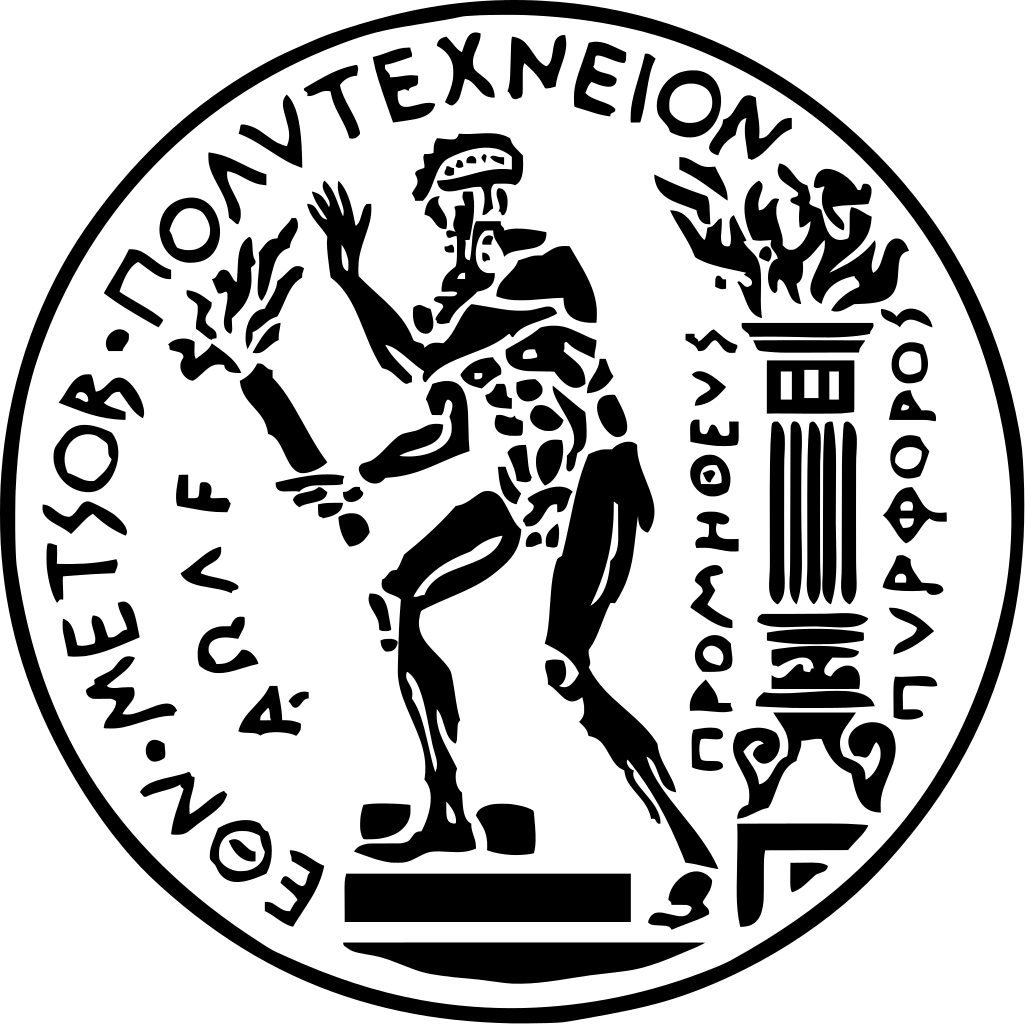
\includegraphics[width=0.3\textwidth]{mets.png}

\vfill
 
Project Submitted in Partial Fulfilment of the\\ Requirements for the Degree of\\ Master of Applied Mechanics
 
\vspace{.8cm}
 

 

National Technical University of Athens\\ 
School of Applied Mathematical and Physical Sciences\\
\today
 
\end{center}
\end{titlepage}

\tableofcontents
\pagebreak

\hline
\begin{abstract}
We study the dynamics of identical leaky integrate-and-fire neurons with symmetric non-local coupling. Upon varying control parameters such as the coupling strength and the coupling range, we investigate the system's behaviour and highlight the formation of chimera states. We also, examine a modified version of the model by varying the coefficient of the leak term.
\end{abstract}
\hline

\section{Introduction}
The study of dynamics and in particular collective behaviour of coupled oscillators has received great interest from scientists in different fields, from chemical systems to neuroscience and beyond. A particularly interesting and unexpected phenomenon observed in coupled oscillators is the so-called \textit{chimera state}. In this dynamical scenario, some oscillators are synchronised while the others are not. These states were first observed in 2002 by Kuramoto and Battogtokh \cite{kuramoto} while the term chimera was coined in 2004 by Abrams and Strogatz \cite{stro}. Potential applications of this phenomenon include the unihemispheric sleep observed in dolphins and some birds, power grids and social systems. This phenomenon has been observed numerically in various neuron models.
\par In this study we examine the effect of different control parameters on the appearance of chimera states for leaky integrate-and-fire (LIF) neuronal oscillators arranged in a regular ring topology. 

\section{The leaky integrate-and-fire model}
\subsection{The single neuron model}
The LIF model is a simple model for spiking neurons introduced in 1907 by Louis Lapicque \cite{tsigkrimulti}. The main dynamical variable is the membrane potential $u(t)$, which evolves according to the equation
\begin{equation} \label{eq1}
\frac{d u(t)}{dt} = \mu - \lambda \, u(t),
\end{equation}
with a reset condition
\begin{equation} \label{eq2}
\forall u(t) = u_{th} \Rightarrow \lim_{\epsilon \rightarrow 0} u(t + \epsilon) = u_{\text{rest}}, 
\end{equation}
where $u_{th}$ is the threshold of the potential, $u_{\text{rest}}$ is the membrane potential at the rest state, and $\mu > u_{th}$ is a constant. The parameter $\lambda$ is set to $\lambda=1$ for the original LIF model, but it is included here because in the last section of this paper we study a modified version of the model. 

\begin{figure}[H]
\centering
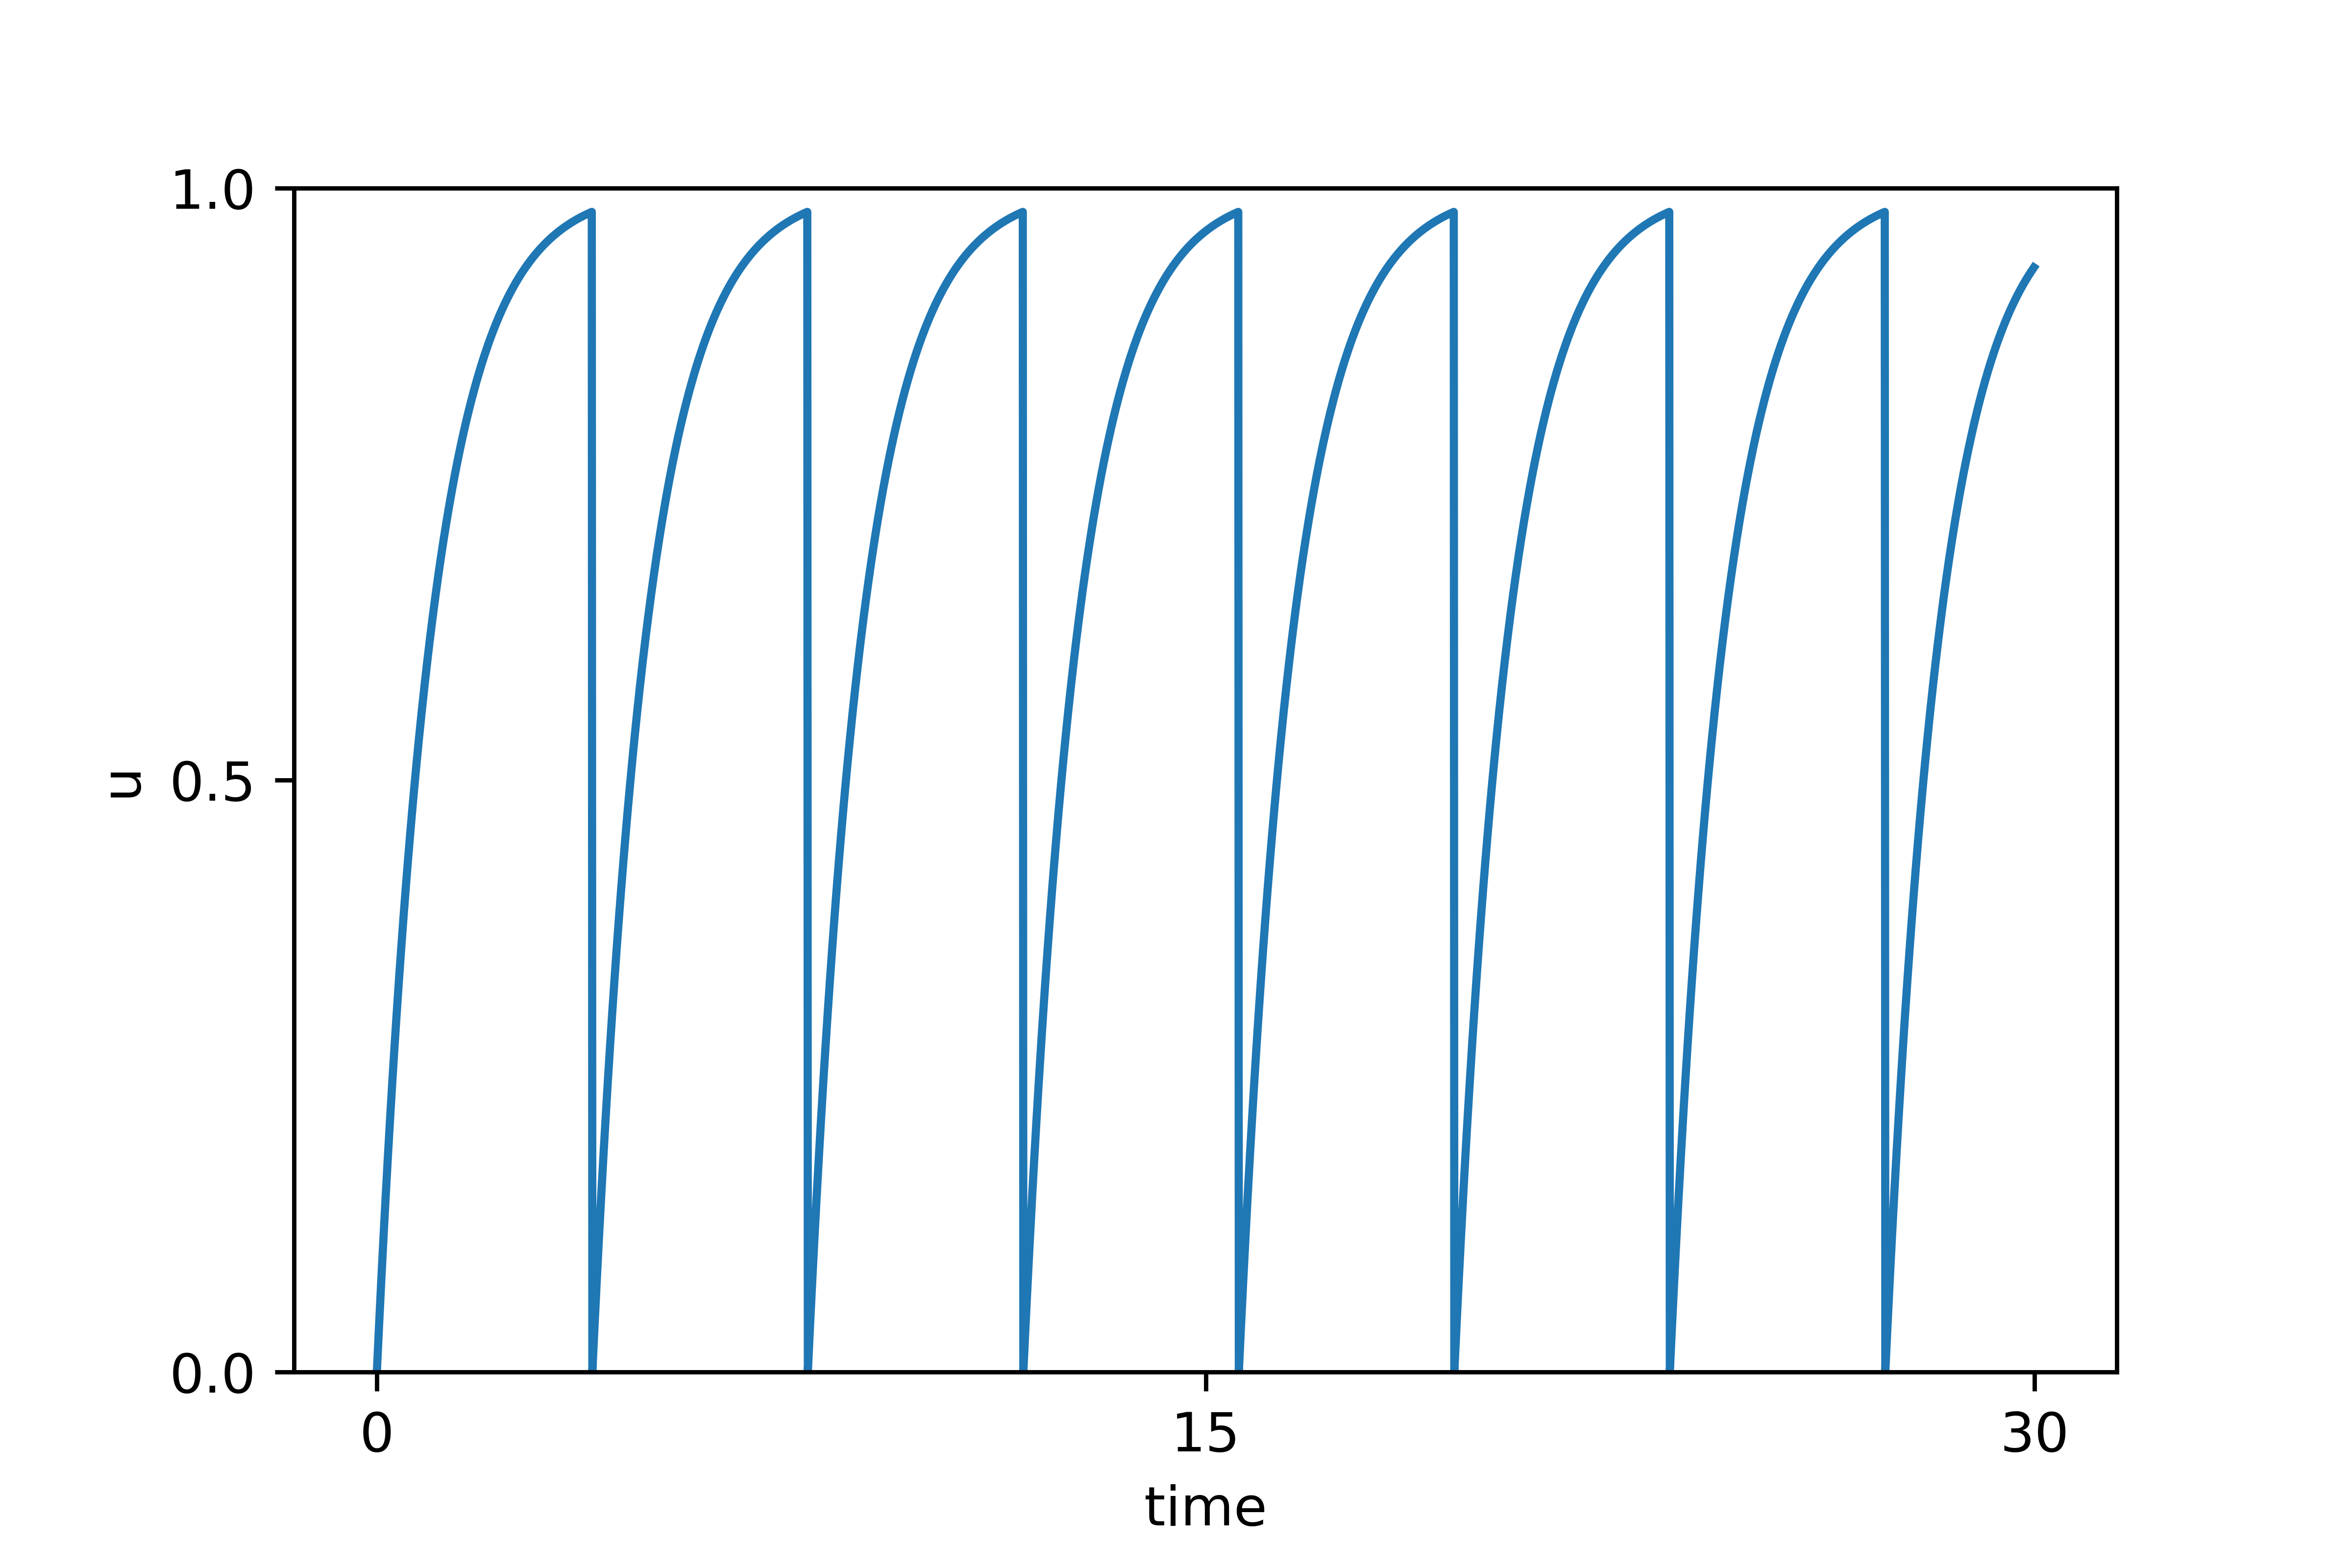
\includegraphics[width=0.8 \textwidth]{lif_single.png}
\caption{Dynamic evolution of the membrane potential in time according to Eq. (\ref{eq1}) and (\ref{eq2}).}
\end{figure}

\par The model, Eq. (\ref{eq1}), includes a leak term, appearing as $-u(t)$ on the right-hand side, and is linear. However, with the addition of the reset condition, Eq. (\ref{eq2}), the model becomes highly non-linear. Whenever the potential reaches the threshold $u_{th}$, it drops to $u_{\text{rest}}$. The resting potential can be set to $u_{\text{rest}}=0$. 

\subsection{Nonlocally coupled network of LIF neurons}
Neurons ``fire'' electrical signals as a result of receiving input from other neurons. Therefore, it is interesting to study networks of coupled neurons. We study a newtork of $N$ LIF neurons that are arranged in a regular ring topology with non-local connections. That is, each element is coupled to its $R$ nearest neighbours on either side. The dynamical evolution of this system is determined by
\begin{equation} \label{eqncon}
\frac{d u_i(t)}{dt} = \mu - \lambda \, u_i + \frac{\sigma}{2 R} \sum_{j=i-R}^{j=i+R} [u_i(t) - u_j(t)],
\end{equation}
with the same reset mechanism for each element as in Eq. (\ref{eq2}). Here, $\sigma$ is the coupling strength and $R$ is the coupling range. The index $i$ has to be taken modulo $N$ due to the topology and all the nodes are consider identical. 
\par The study of a system of coupled oscillators involves the identification of parameter regions where synchronisation occurs. In the next sections, we investigate the effect of the coupling strength $\sigma$ and the coupling range $R$ on synchronisation phenomena with special focus on chimera states. 


\section{Methods}
The calculations were performed on a conventional PC and coded in Python (Python version 3.8.5) and the total processing time was $\approx 240$ hours. The code was verified by reproducing some of the results in \cite{tsigkrimulti}, \cite{tsigkrimulti2} and \cite{tsigkrichim}. All the scripts used are based on variations of the code in the Appendix. The method used to integrate the ODE is a forward Euler method, with a step size of $dt = 0.01$.

\section{Chimera states in coupled LIF neurons}
We investigate the appearance of chimera states in a network of neurons without refractory period. The model used is the original LIF model, i.e. Eq. (\ref{eq1}) and (\ref{eq2}) with $\lambda = 1$.


\subsection{Minimum number of neurons and $\Delta \omega$ vs $N$}
We study systems with $N=10$, $20$, $30$, $\dots$, $100$, with $r=R/N=0.4$ and $\sigma = 0.7$. Some snapshots are shown in Fig. (\ref{vsN}) and (\ref{vsN2}).
\begin{figure}[H]
\begin{subfigure}{.32\textwidth}
  \centering
  % include first image
  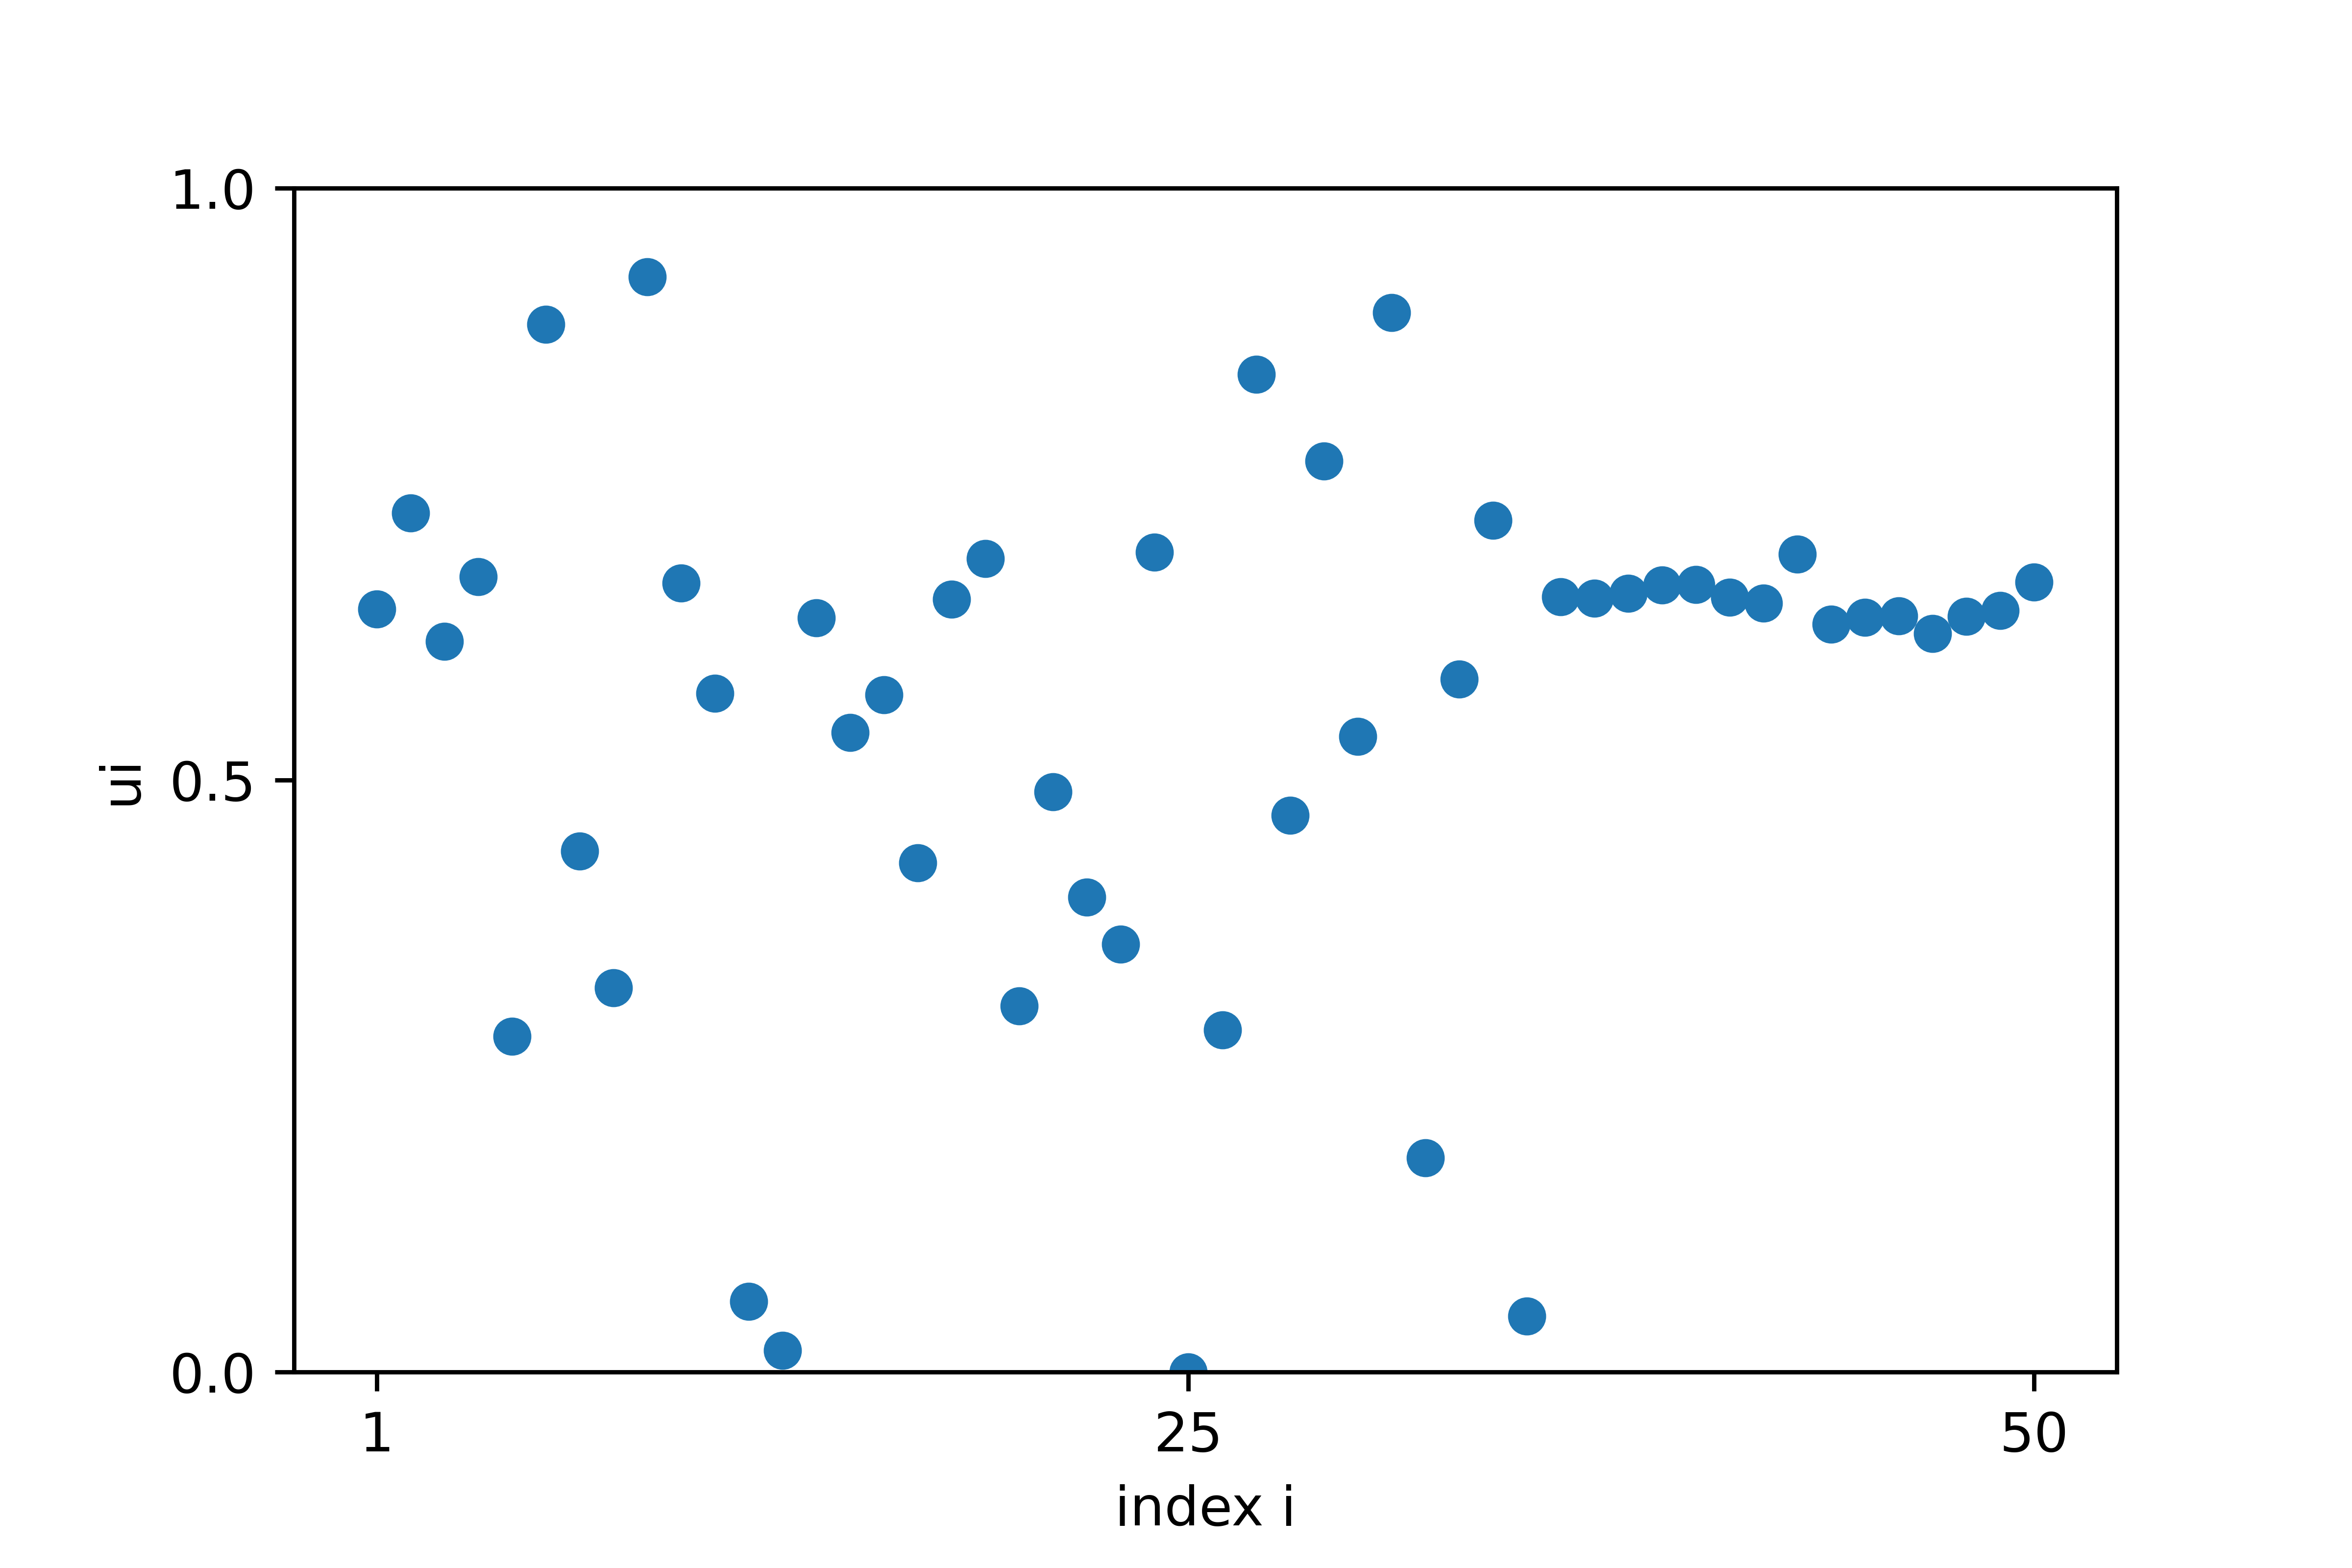
\includegraphics[width=1\linewidth]{u_N=50.png}  
  \caption{$N=50$}
\end{subfigure}
\hfill
\begin{subfigure}{.32\textwidth}
  \centering
  % include second image
  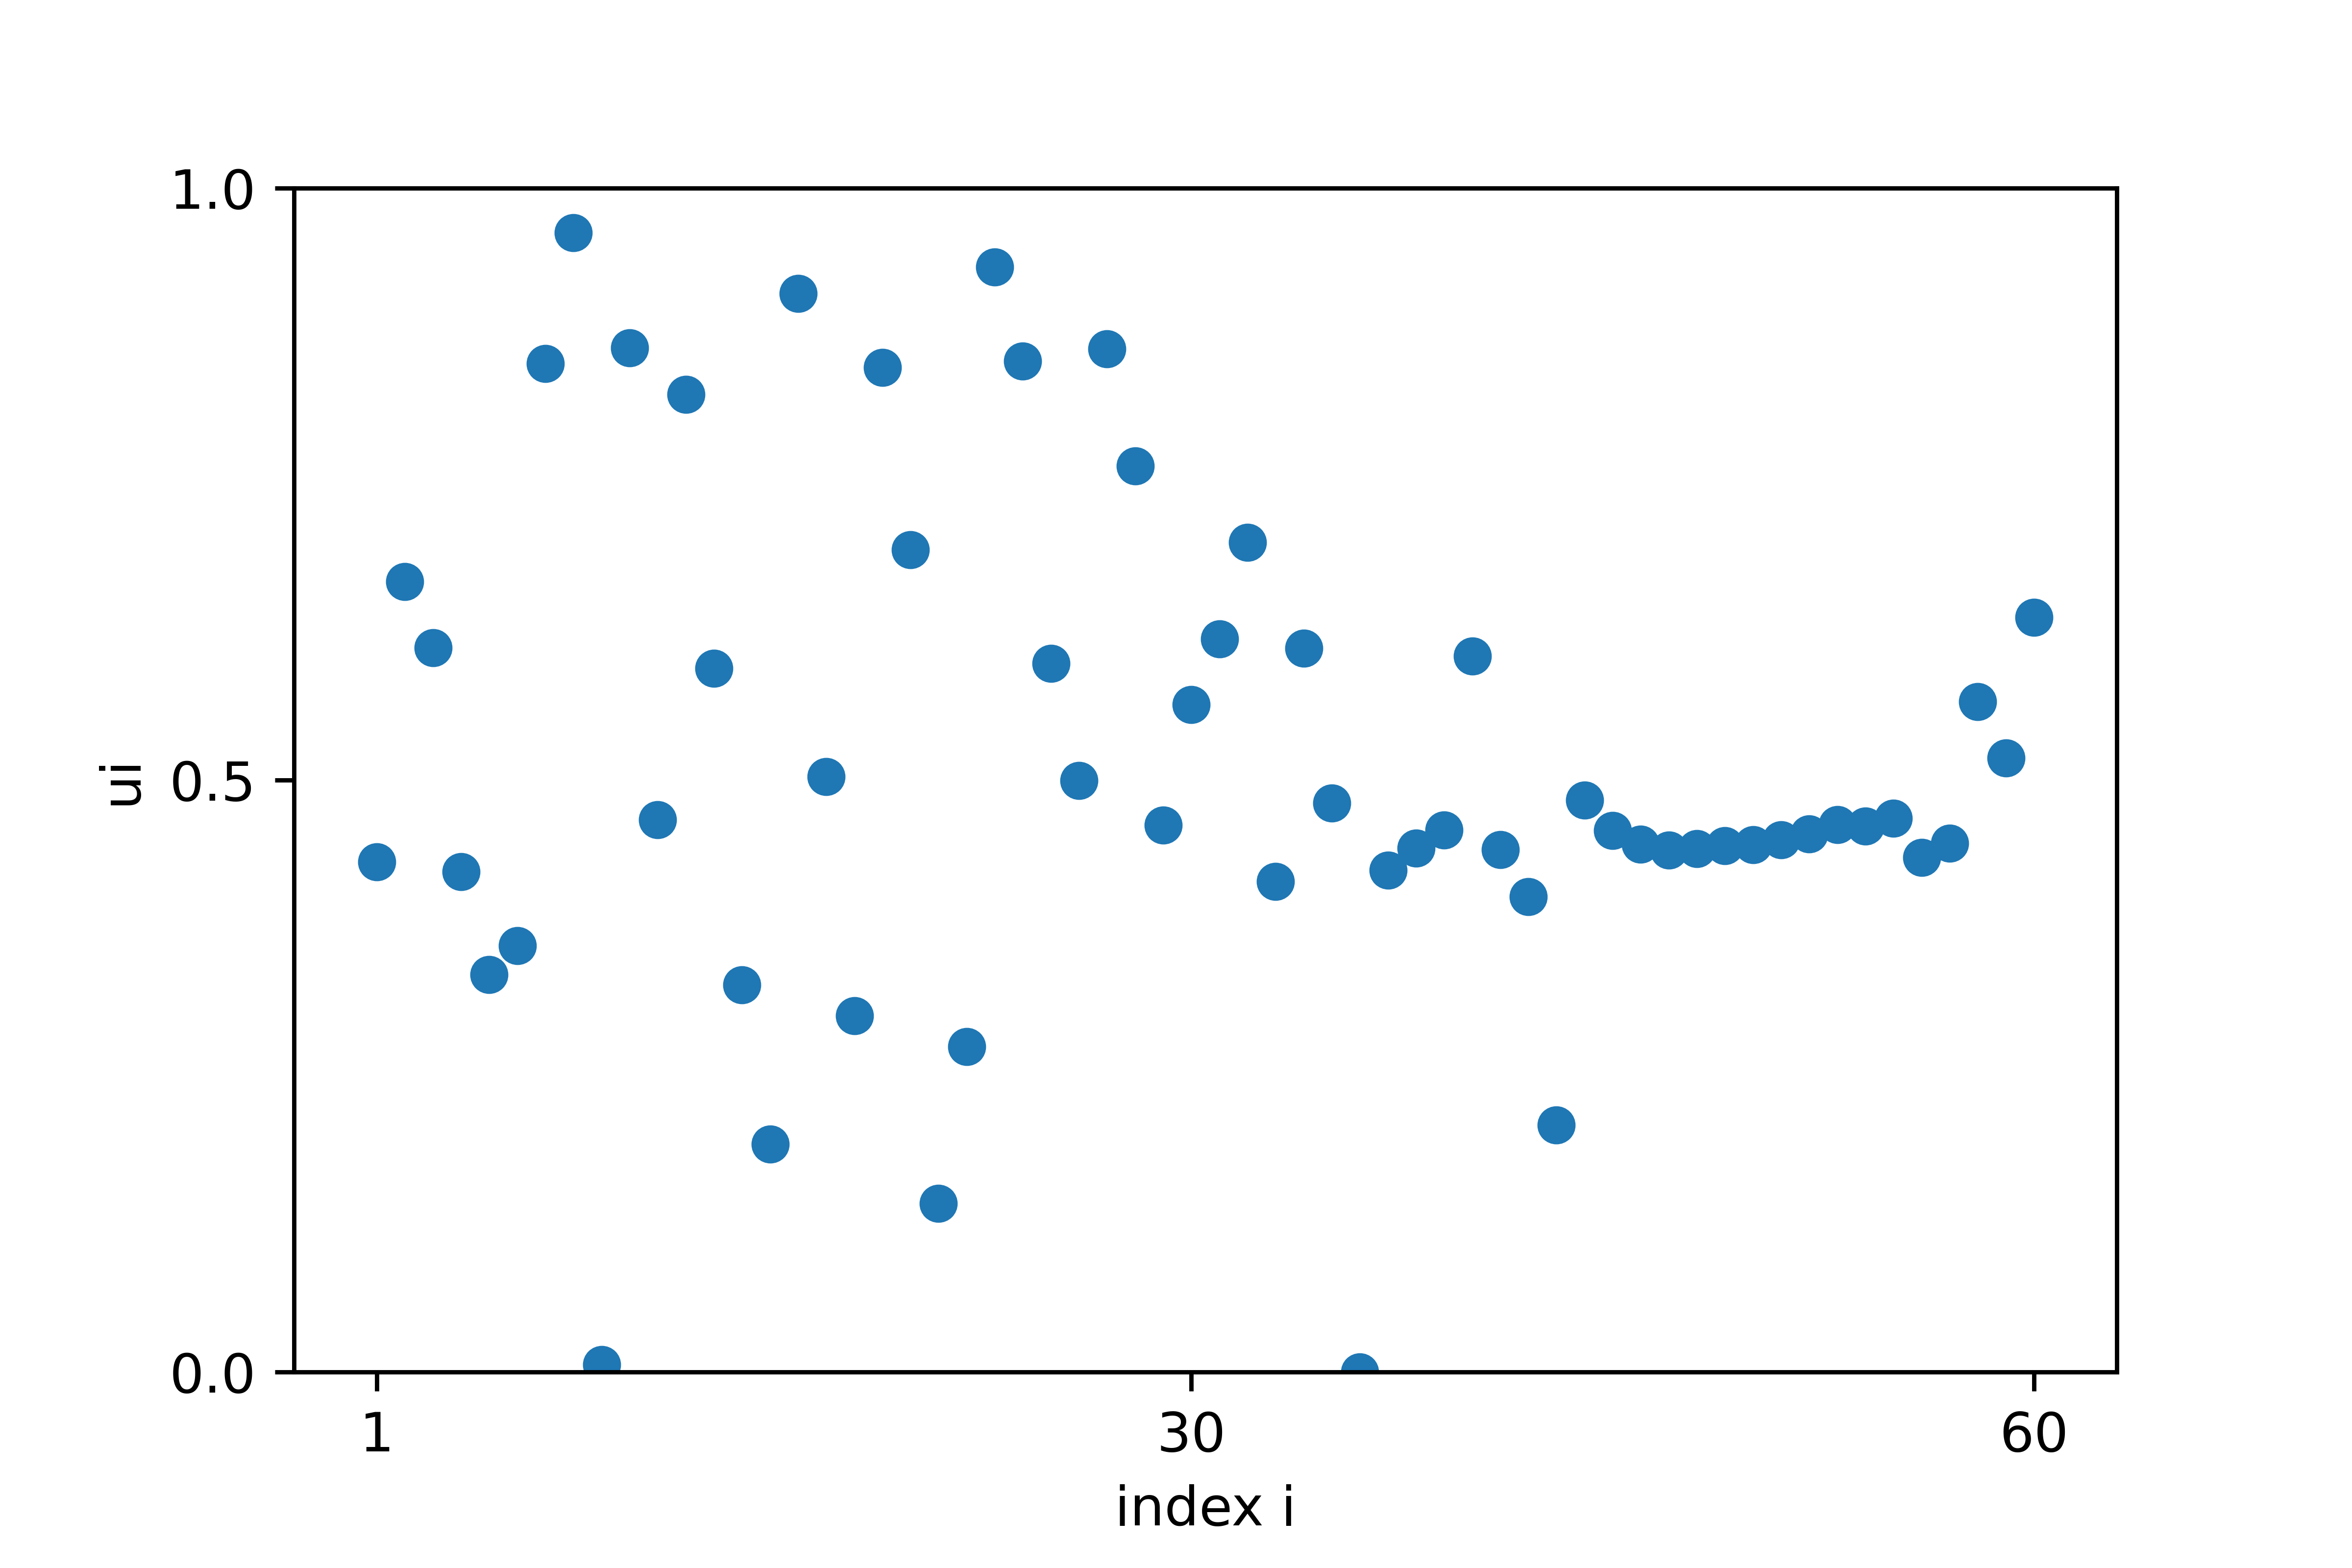
\includegraphics[width=1\linewidth]{u_N=60.png}  
  \caption{$N=60$}
\end{subfigure}
\hfill
\begin{subfigure}{.32\textwidth}
  \centering
  % include first image
  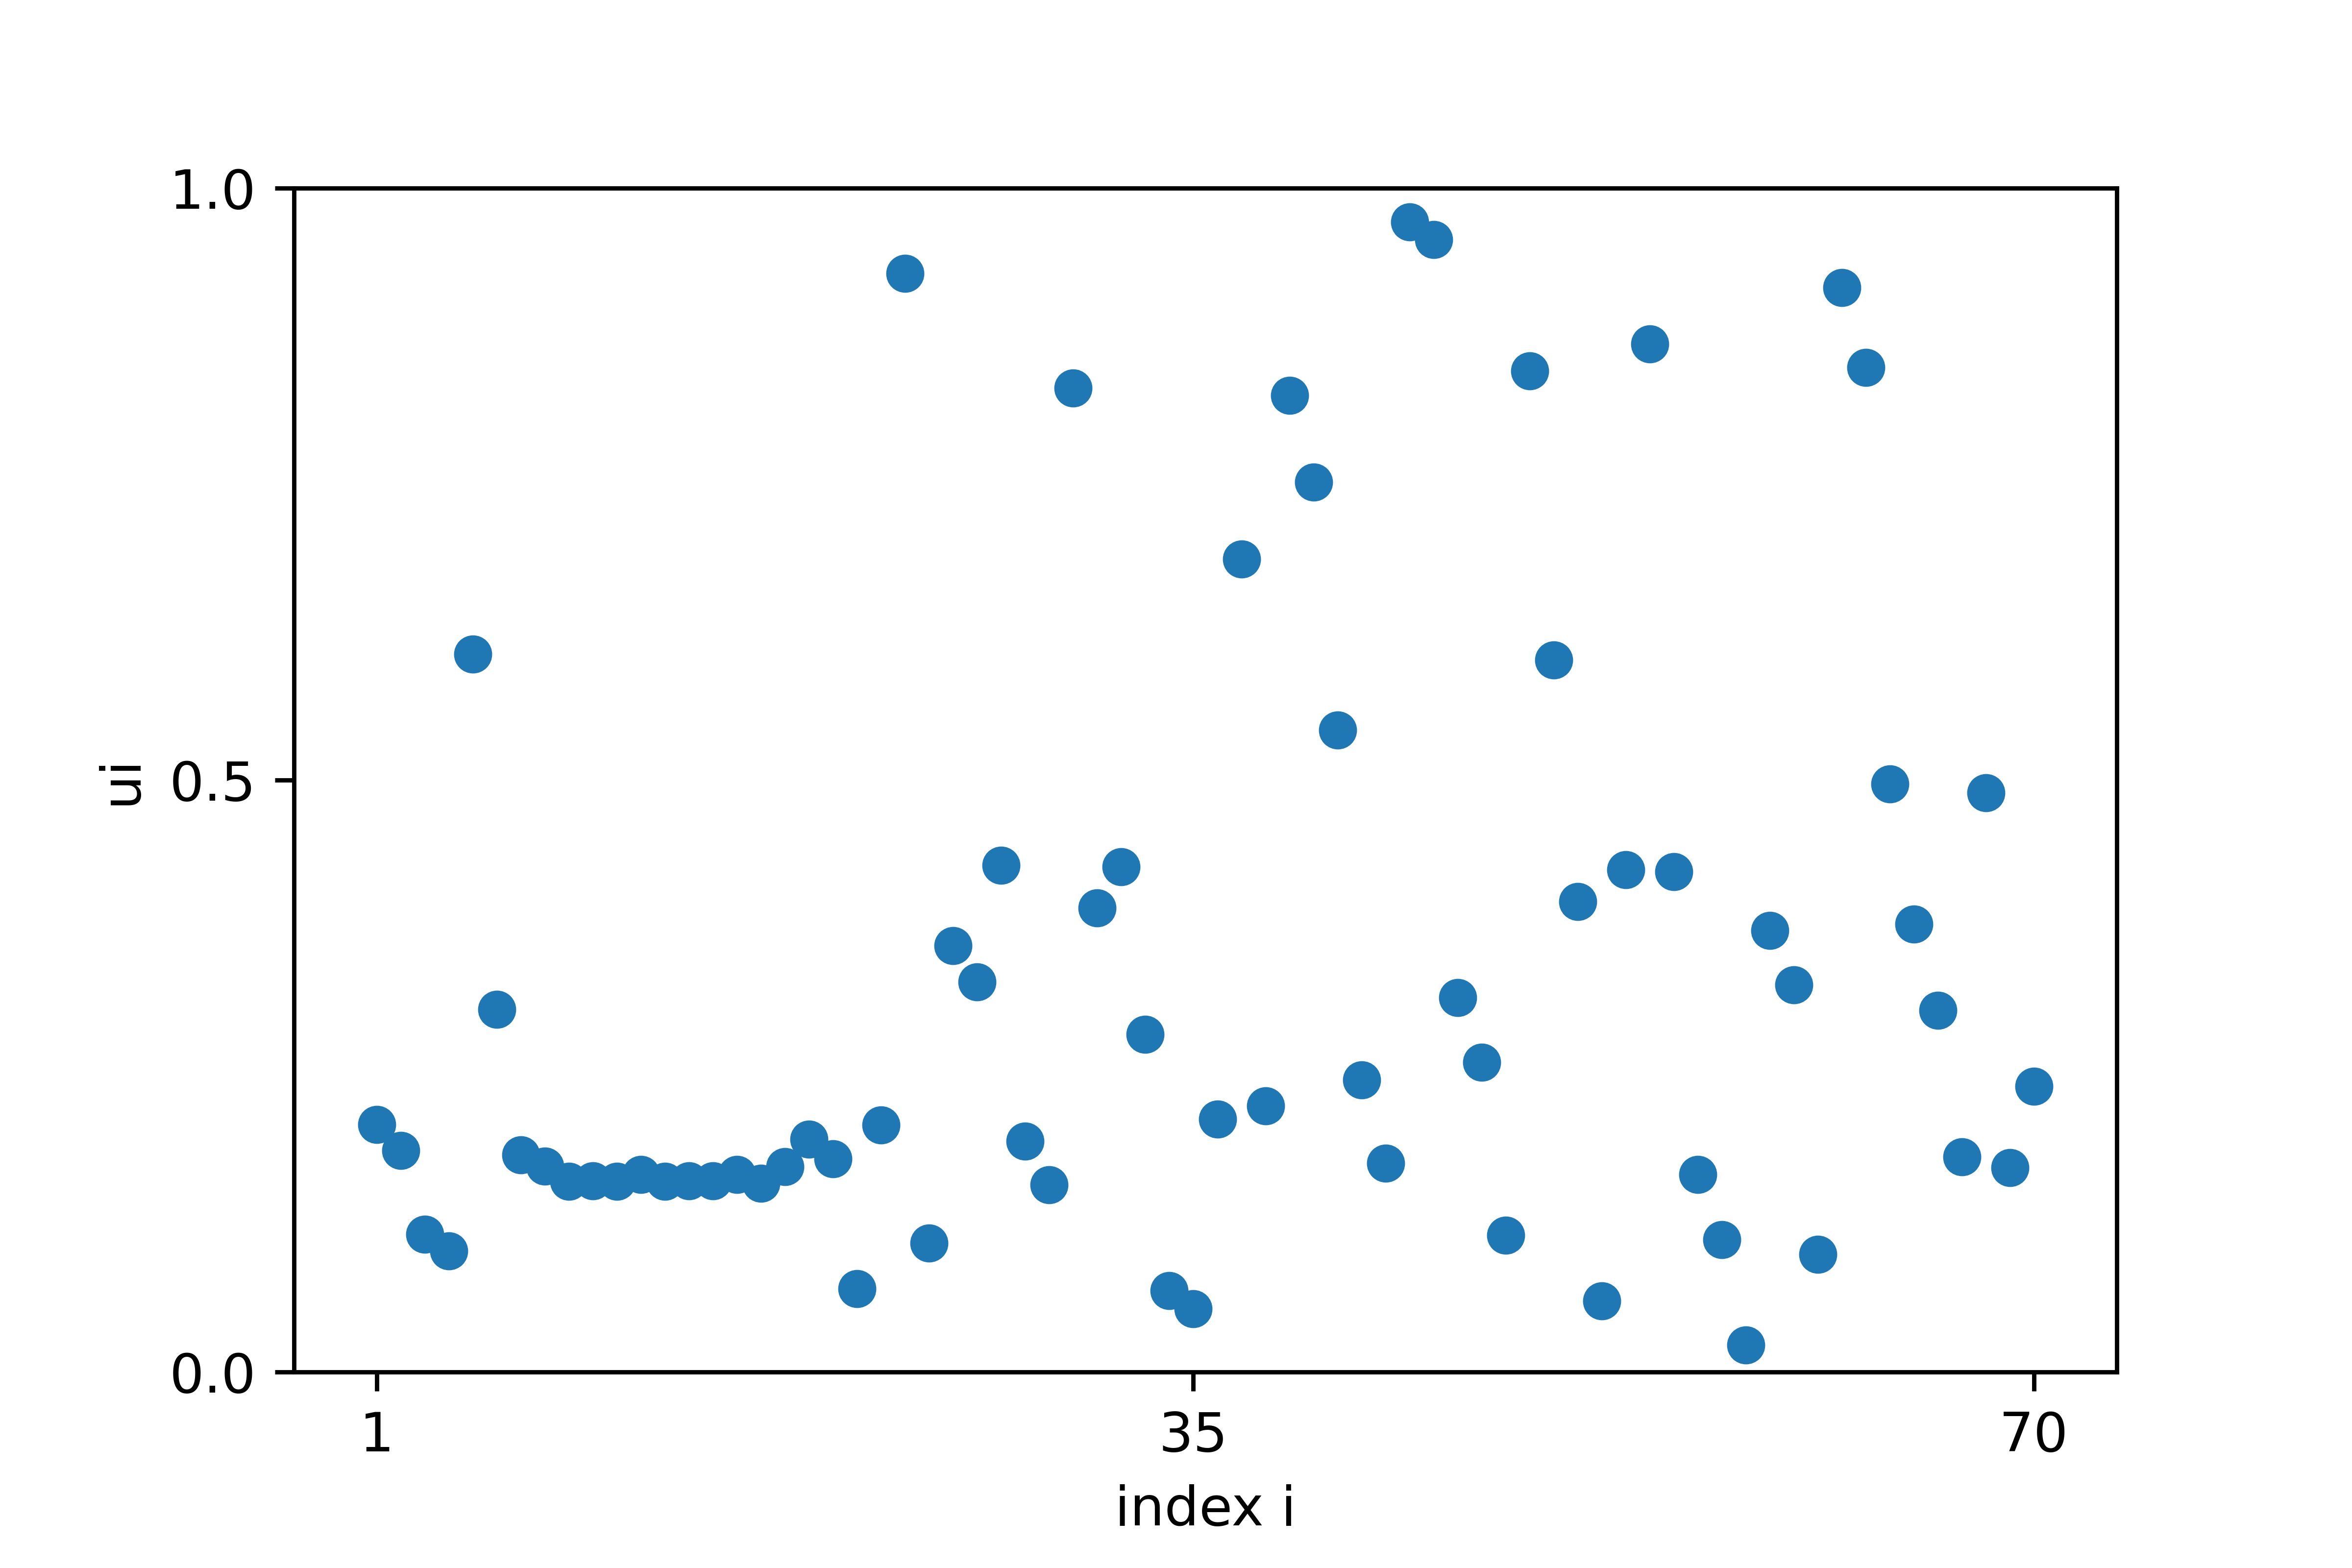
\includegraphics[width=1\linewidth]{u_N=70.png}  
  \caption{$N=70$}
\end{subfigure}
\begin{subfigure}{.32\textwidth}
  \centering
  % include first image
  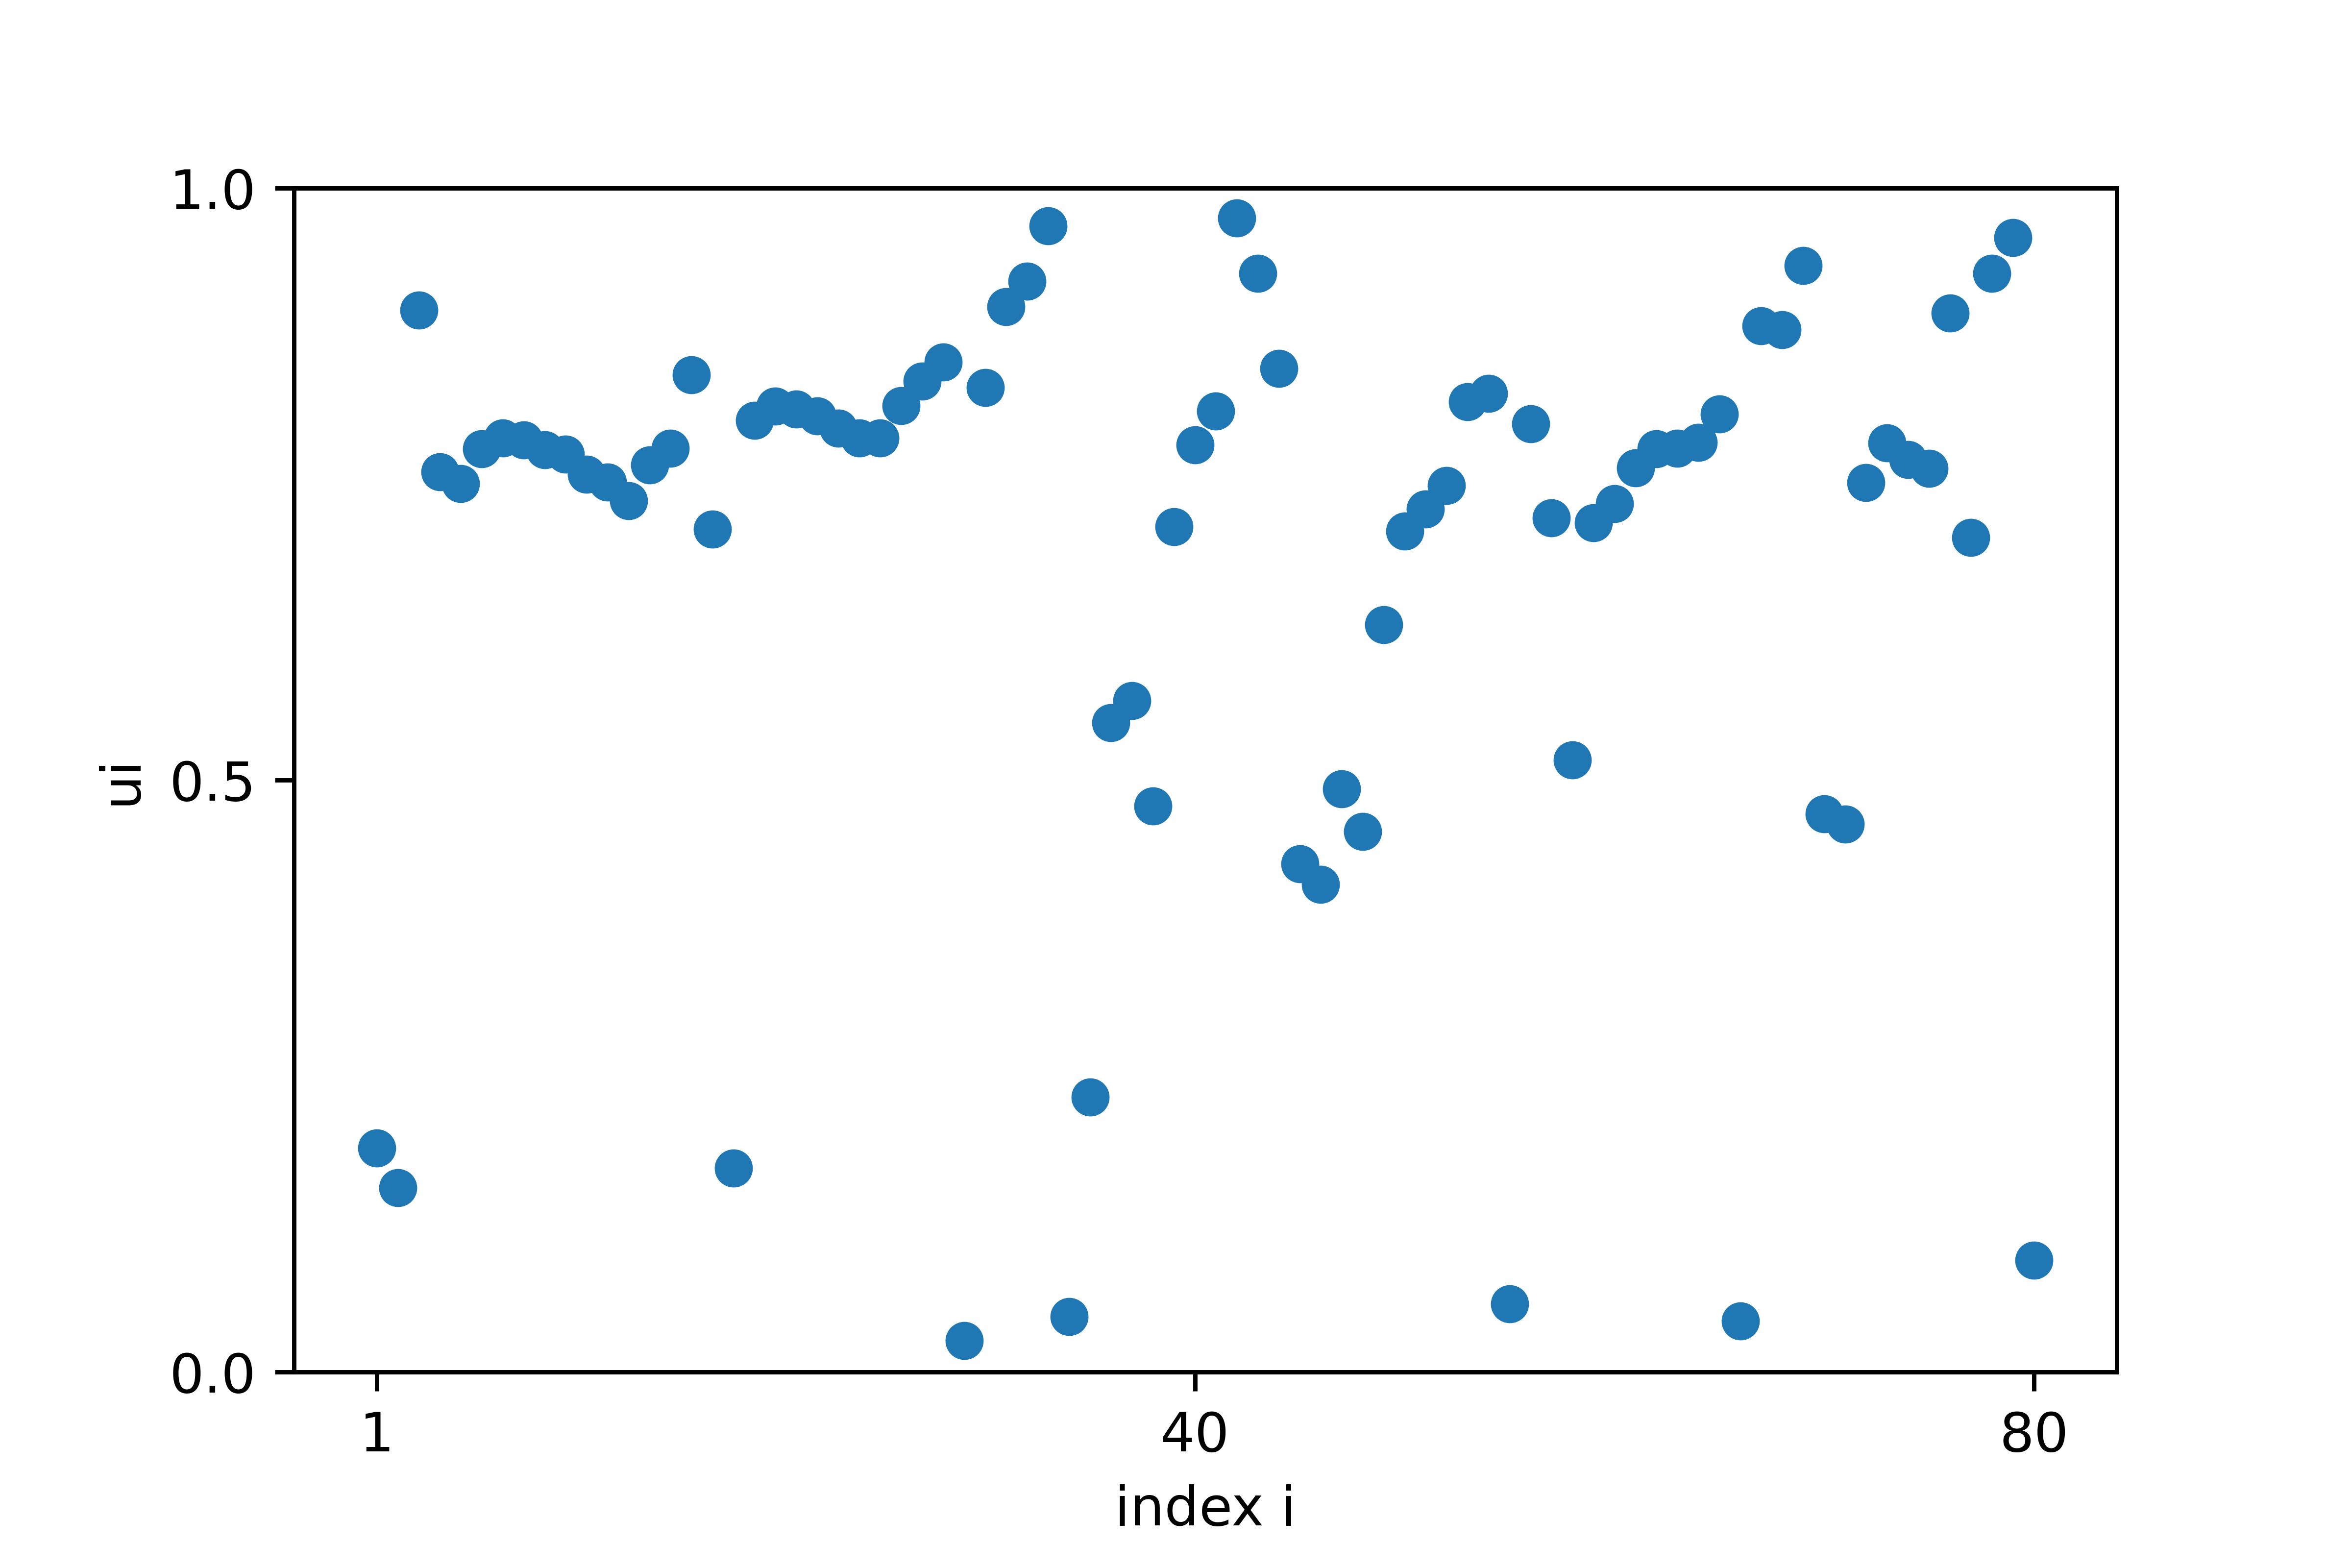
\includegraphics[width=1\linewidth]{u_N=80.png}  
  \caption{$N=80$}
\end{subfigure}
\hfill
\begin{subfigure}{.32\textwidth}
  \centering
  % include first image
  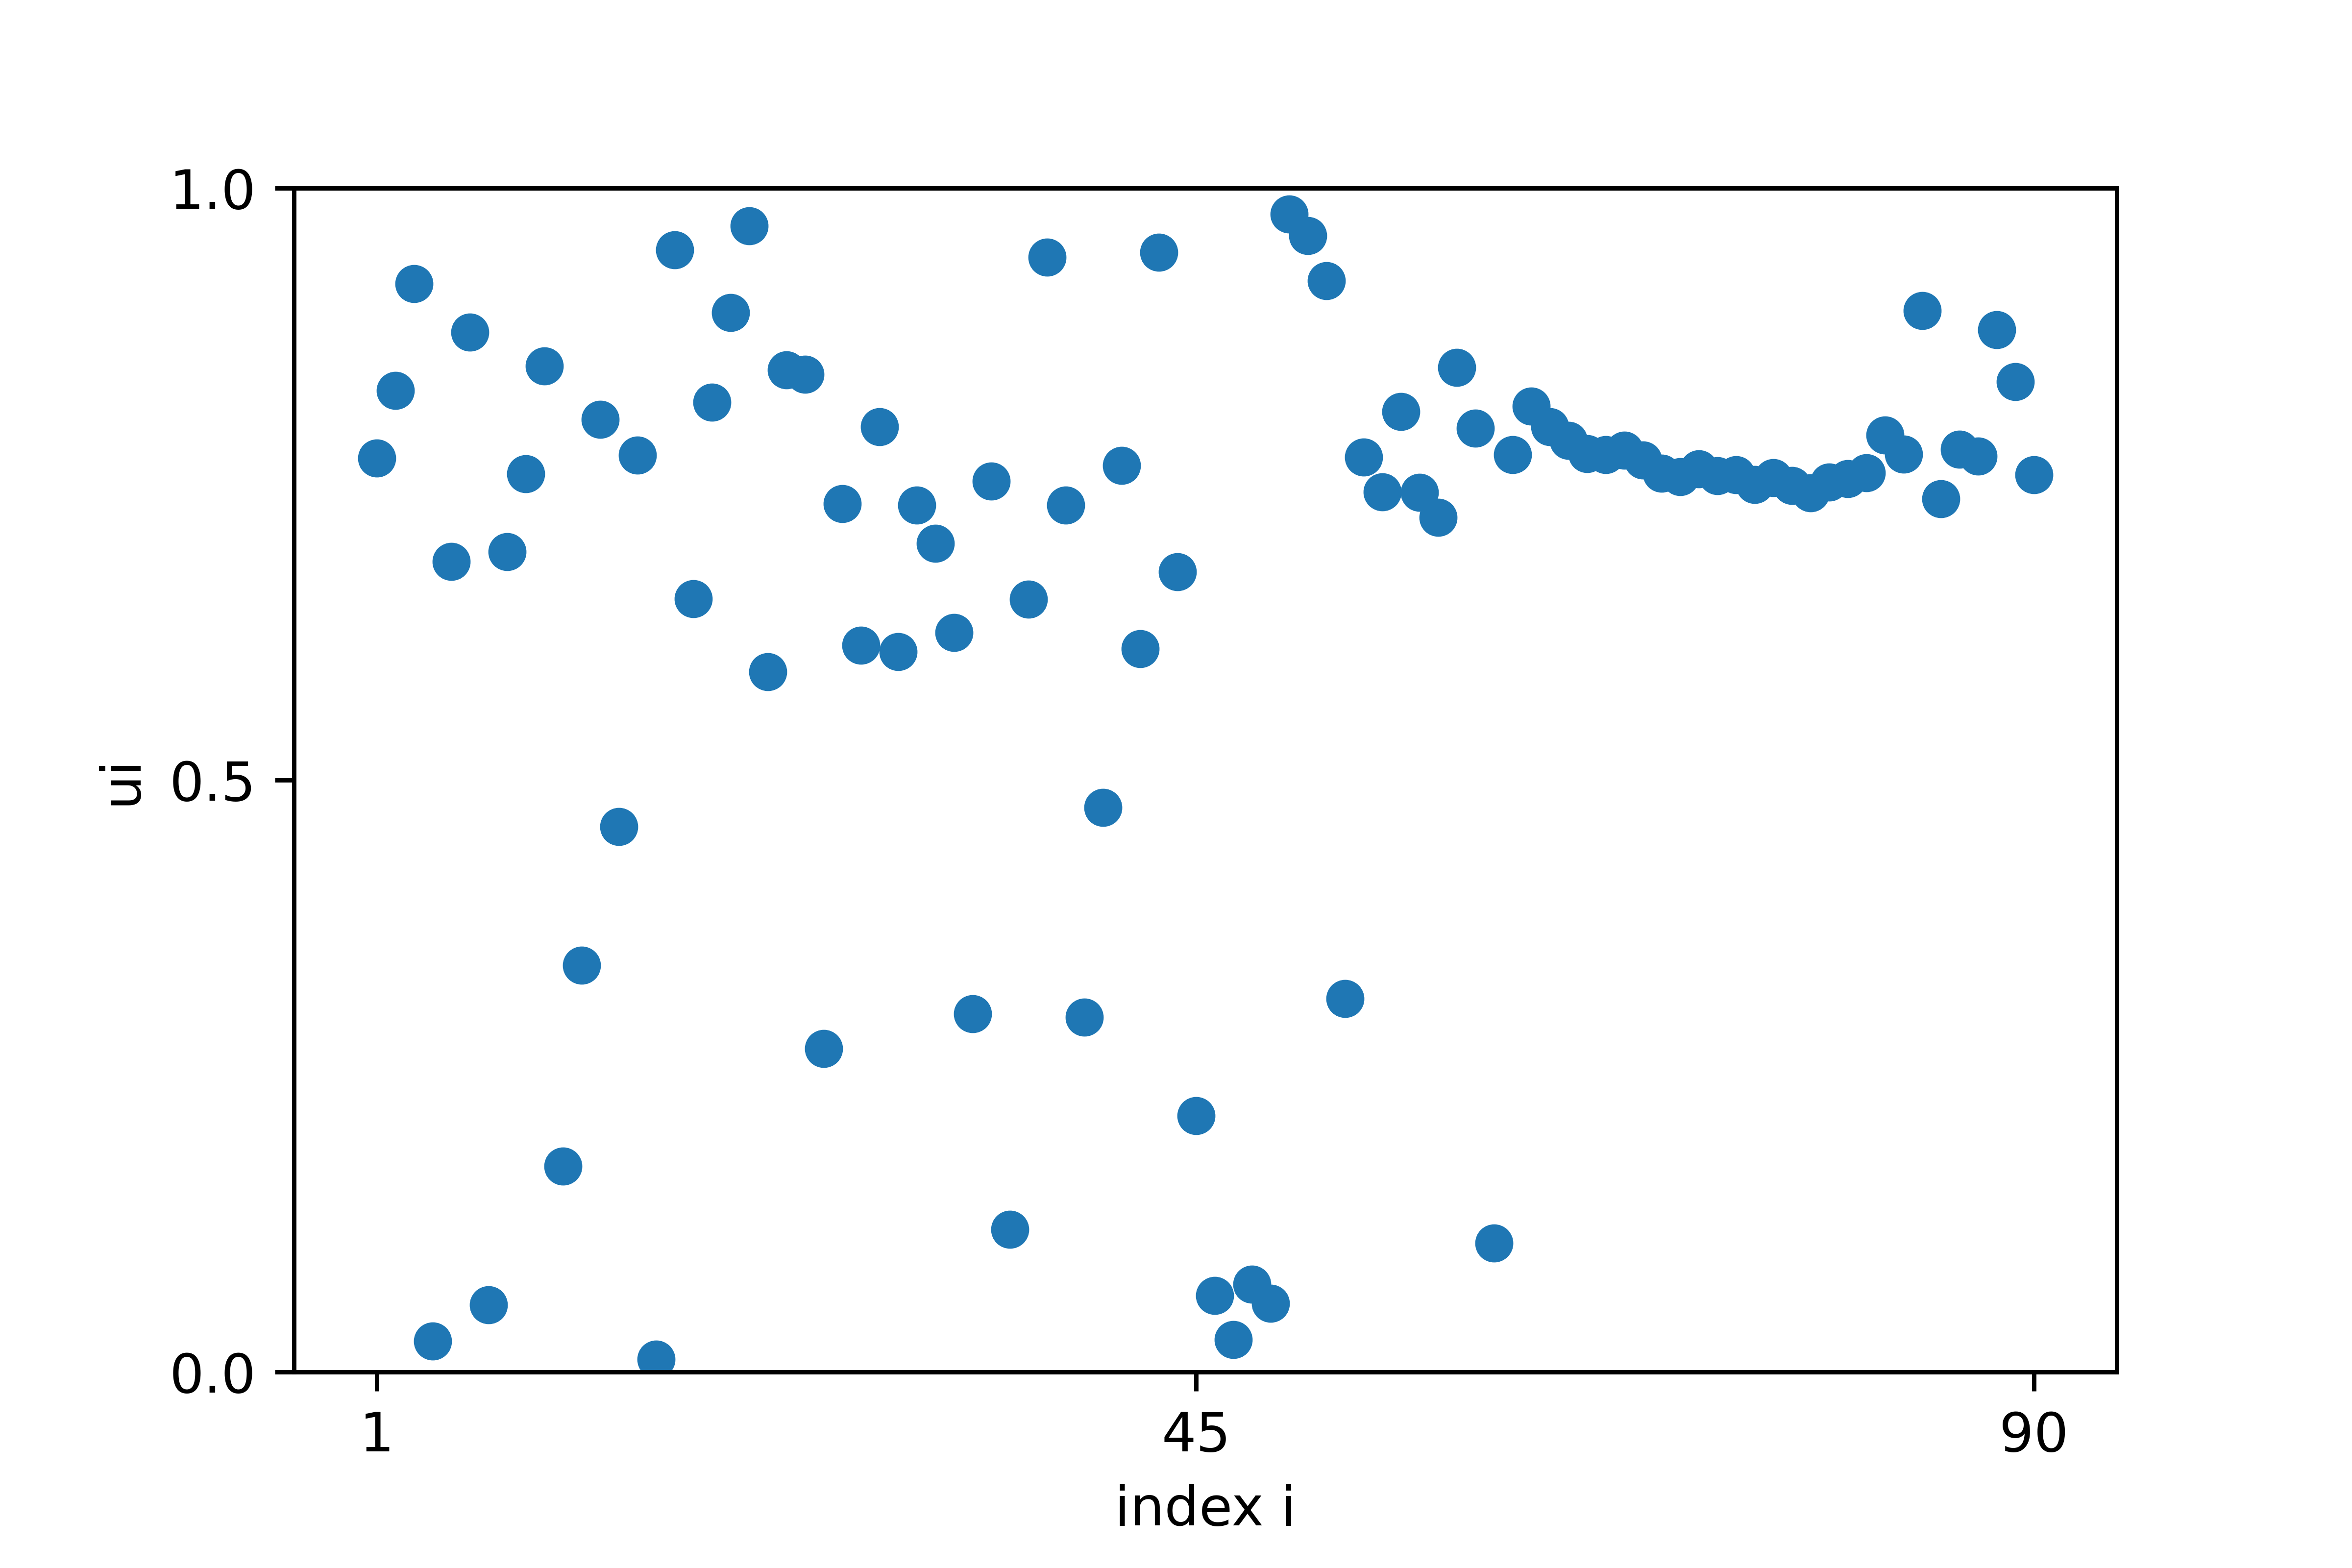
\includegraphics[width=1\linewidth]{u_N=90.png}  
  \caption{$N=90$}
\end{subfigure}
\hfill
\begin{subfigure}{.32\textwidth}
  \centering
  % include first image
  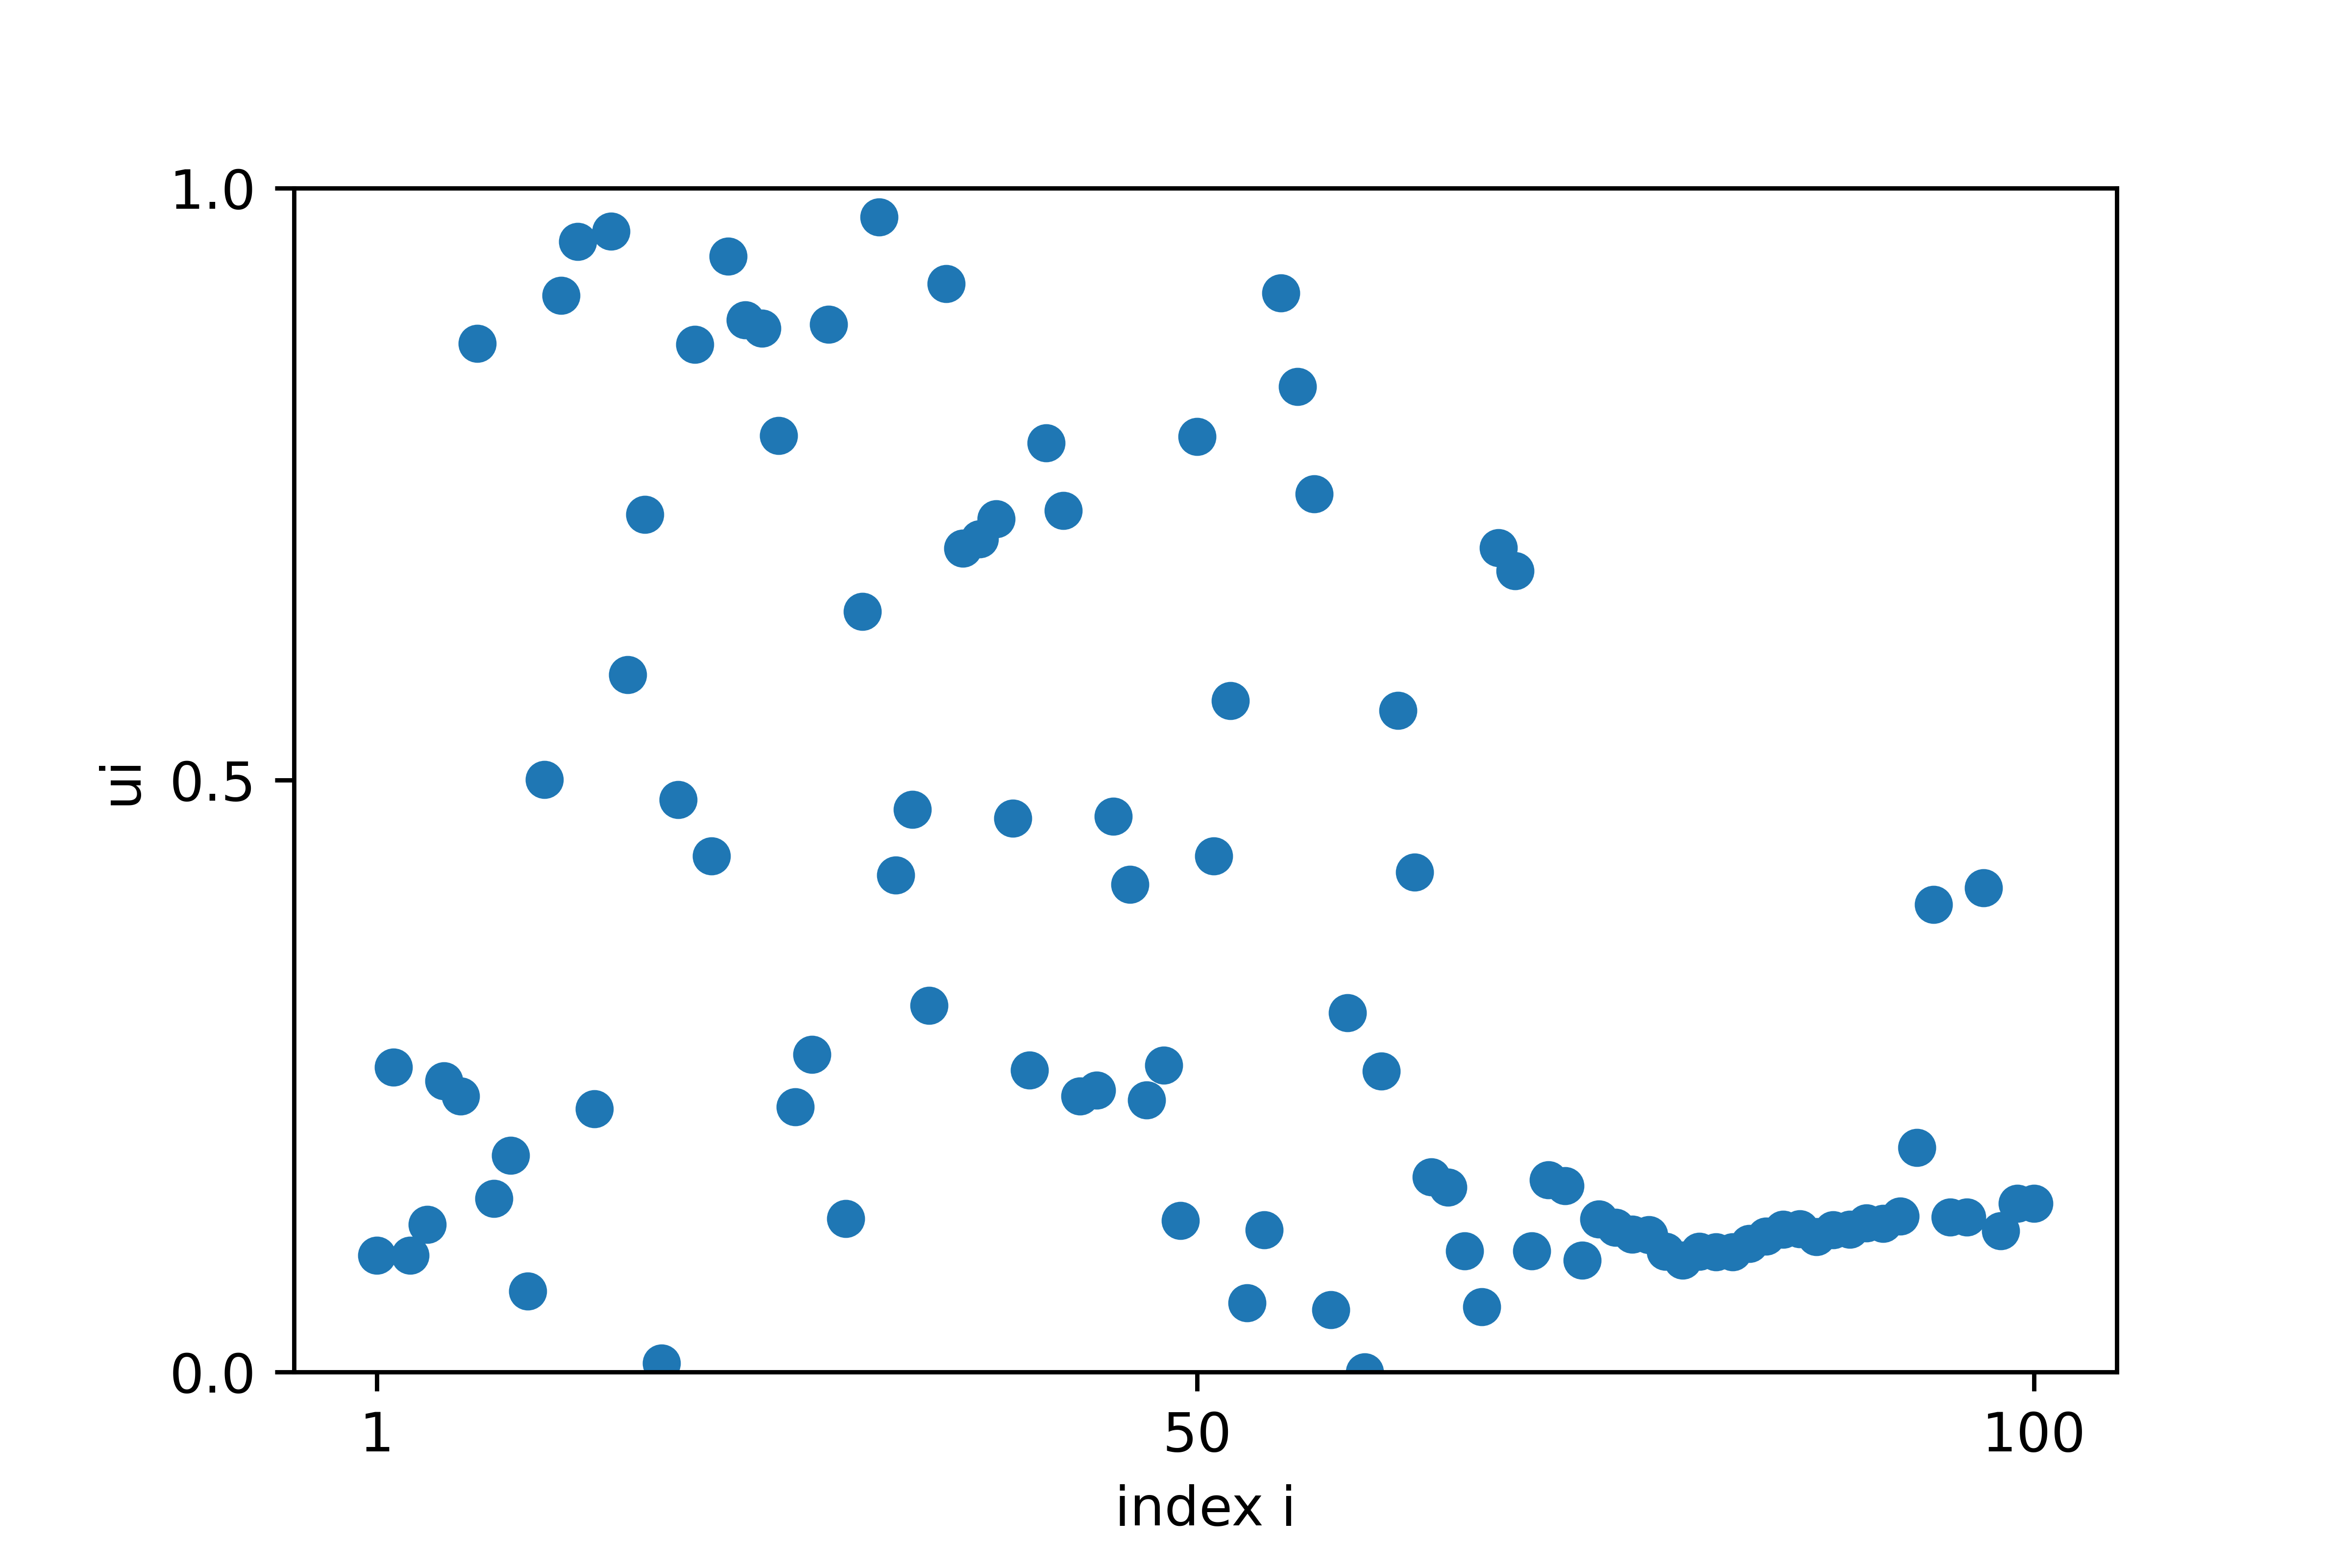
\includegraphics[width=1\linewidth]{u_N=100.png}  
  \caption{$N=100$}
\end{subfigure}
\caption{Snapshots of the membrane potential $u_i$ at $t=1000$ time units, for $\sigma = 0.7$, $r=0.40$ and for various values of $N$.}
\label{vsN}
\end{figure}

\begin{figure}[H]
\begin{subfigure}{.32\textwidth}
  \centering
  % include first image
  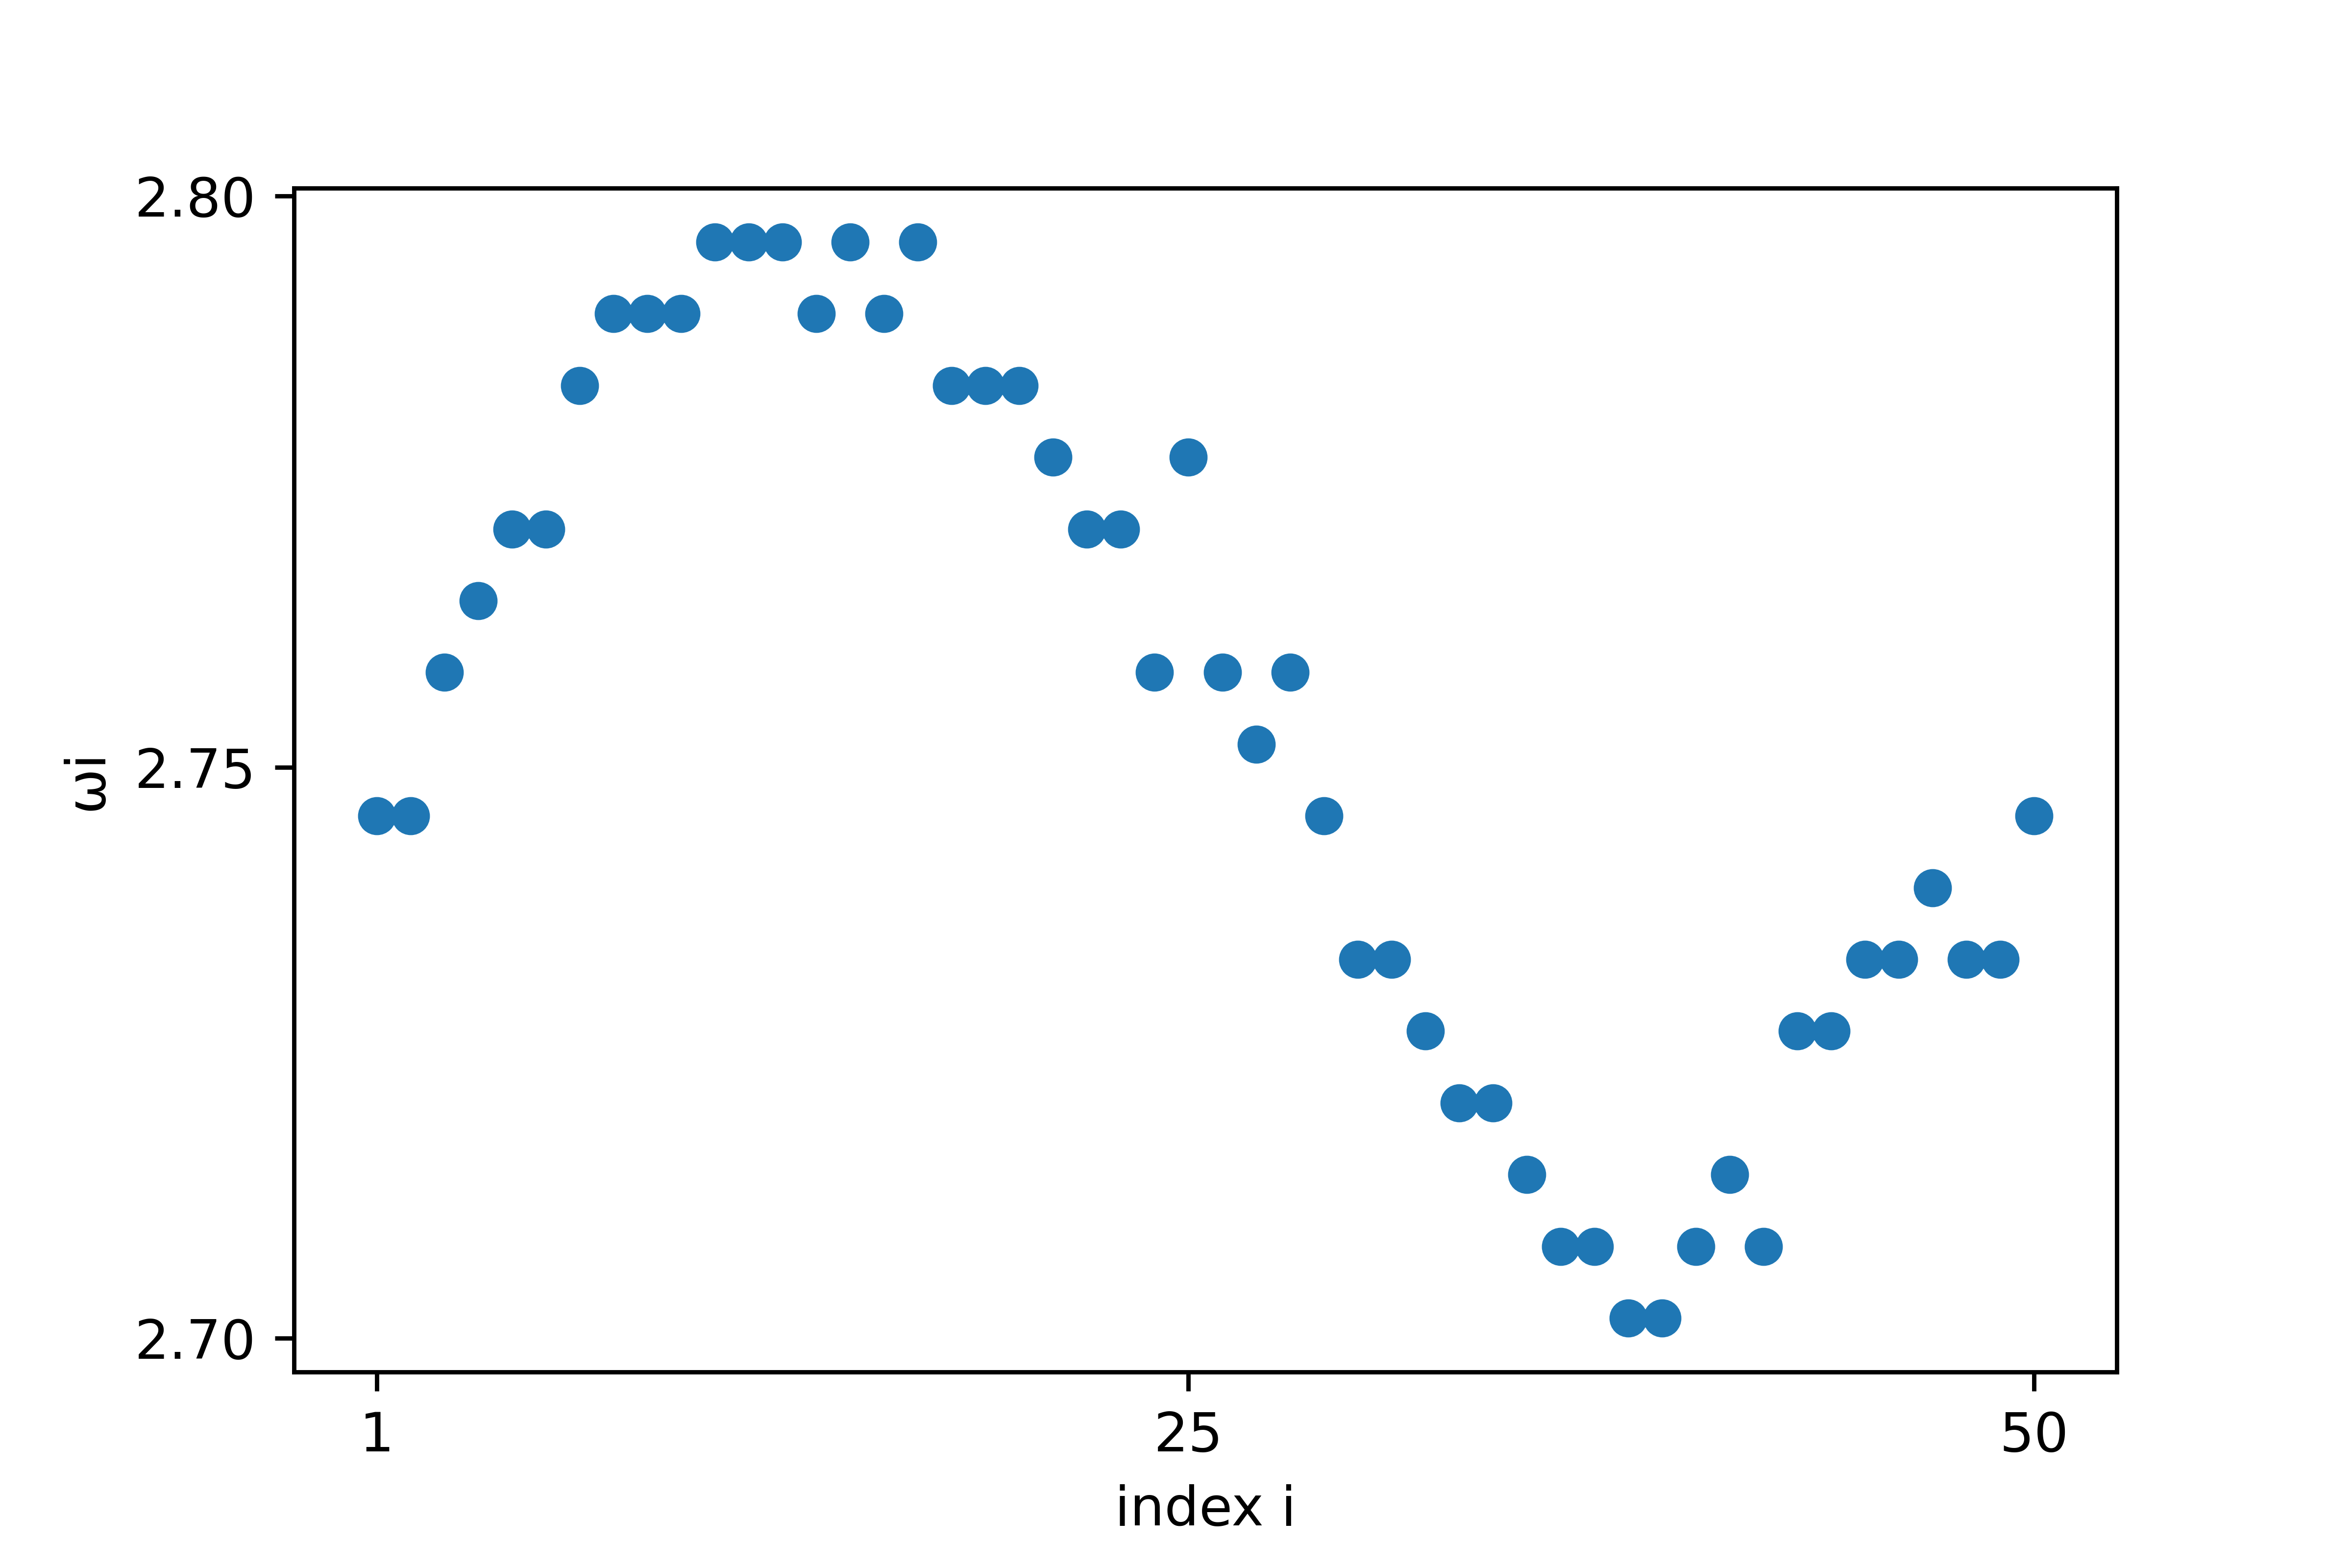
\includegraphics[width=1\linewidth]{w_N=50.png}  
  \caption{$N=50$}
\end{subfigure}
\hfill
\begin{subfigure}{.32\textwidth}
  \centering
  % include second image
  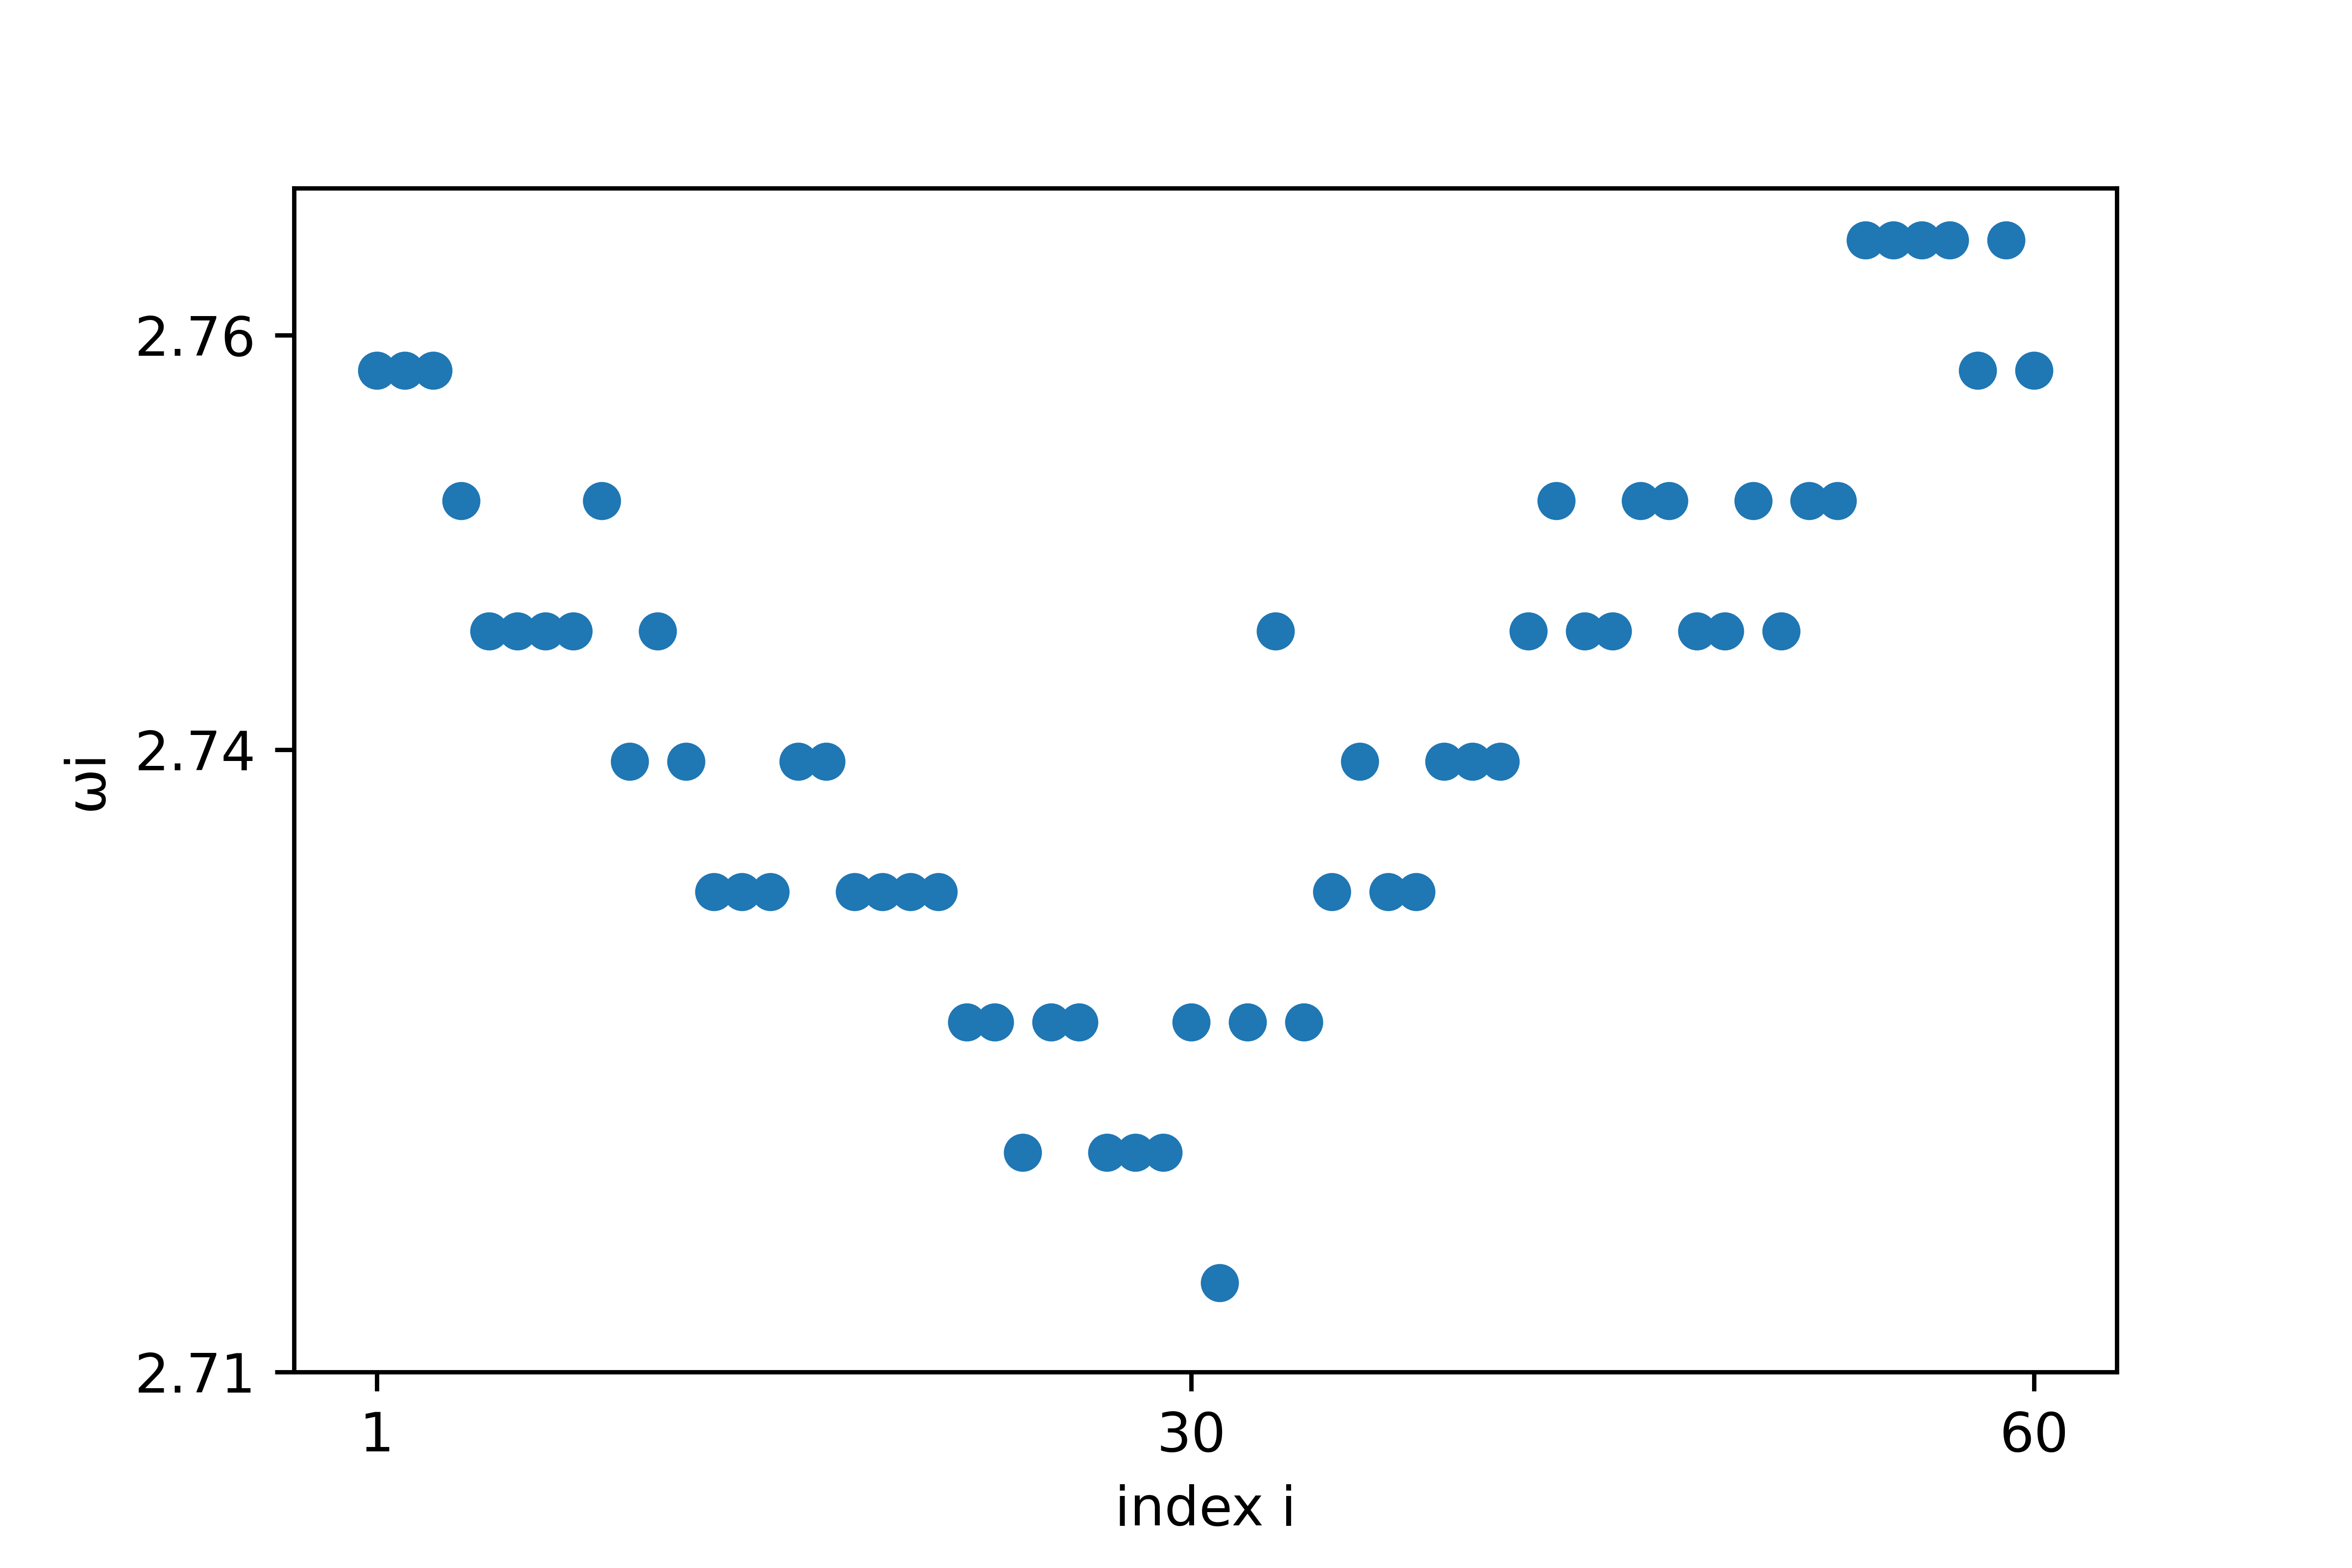
\includegraphics[width=1\linewidth]{w_N=60.png}  
  \caption{$N=60$}
\end{subfigure}
\hfill
\begin{subfigure}{.32\textwidth}
  \centering
  % include first image
  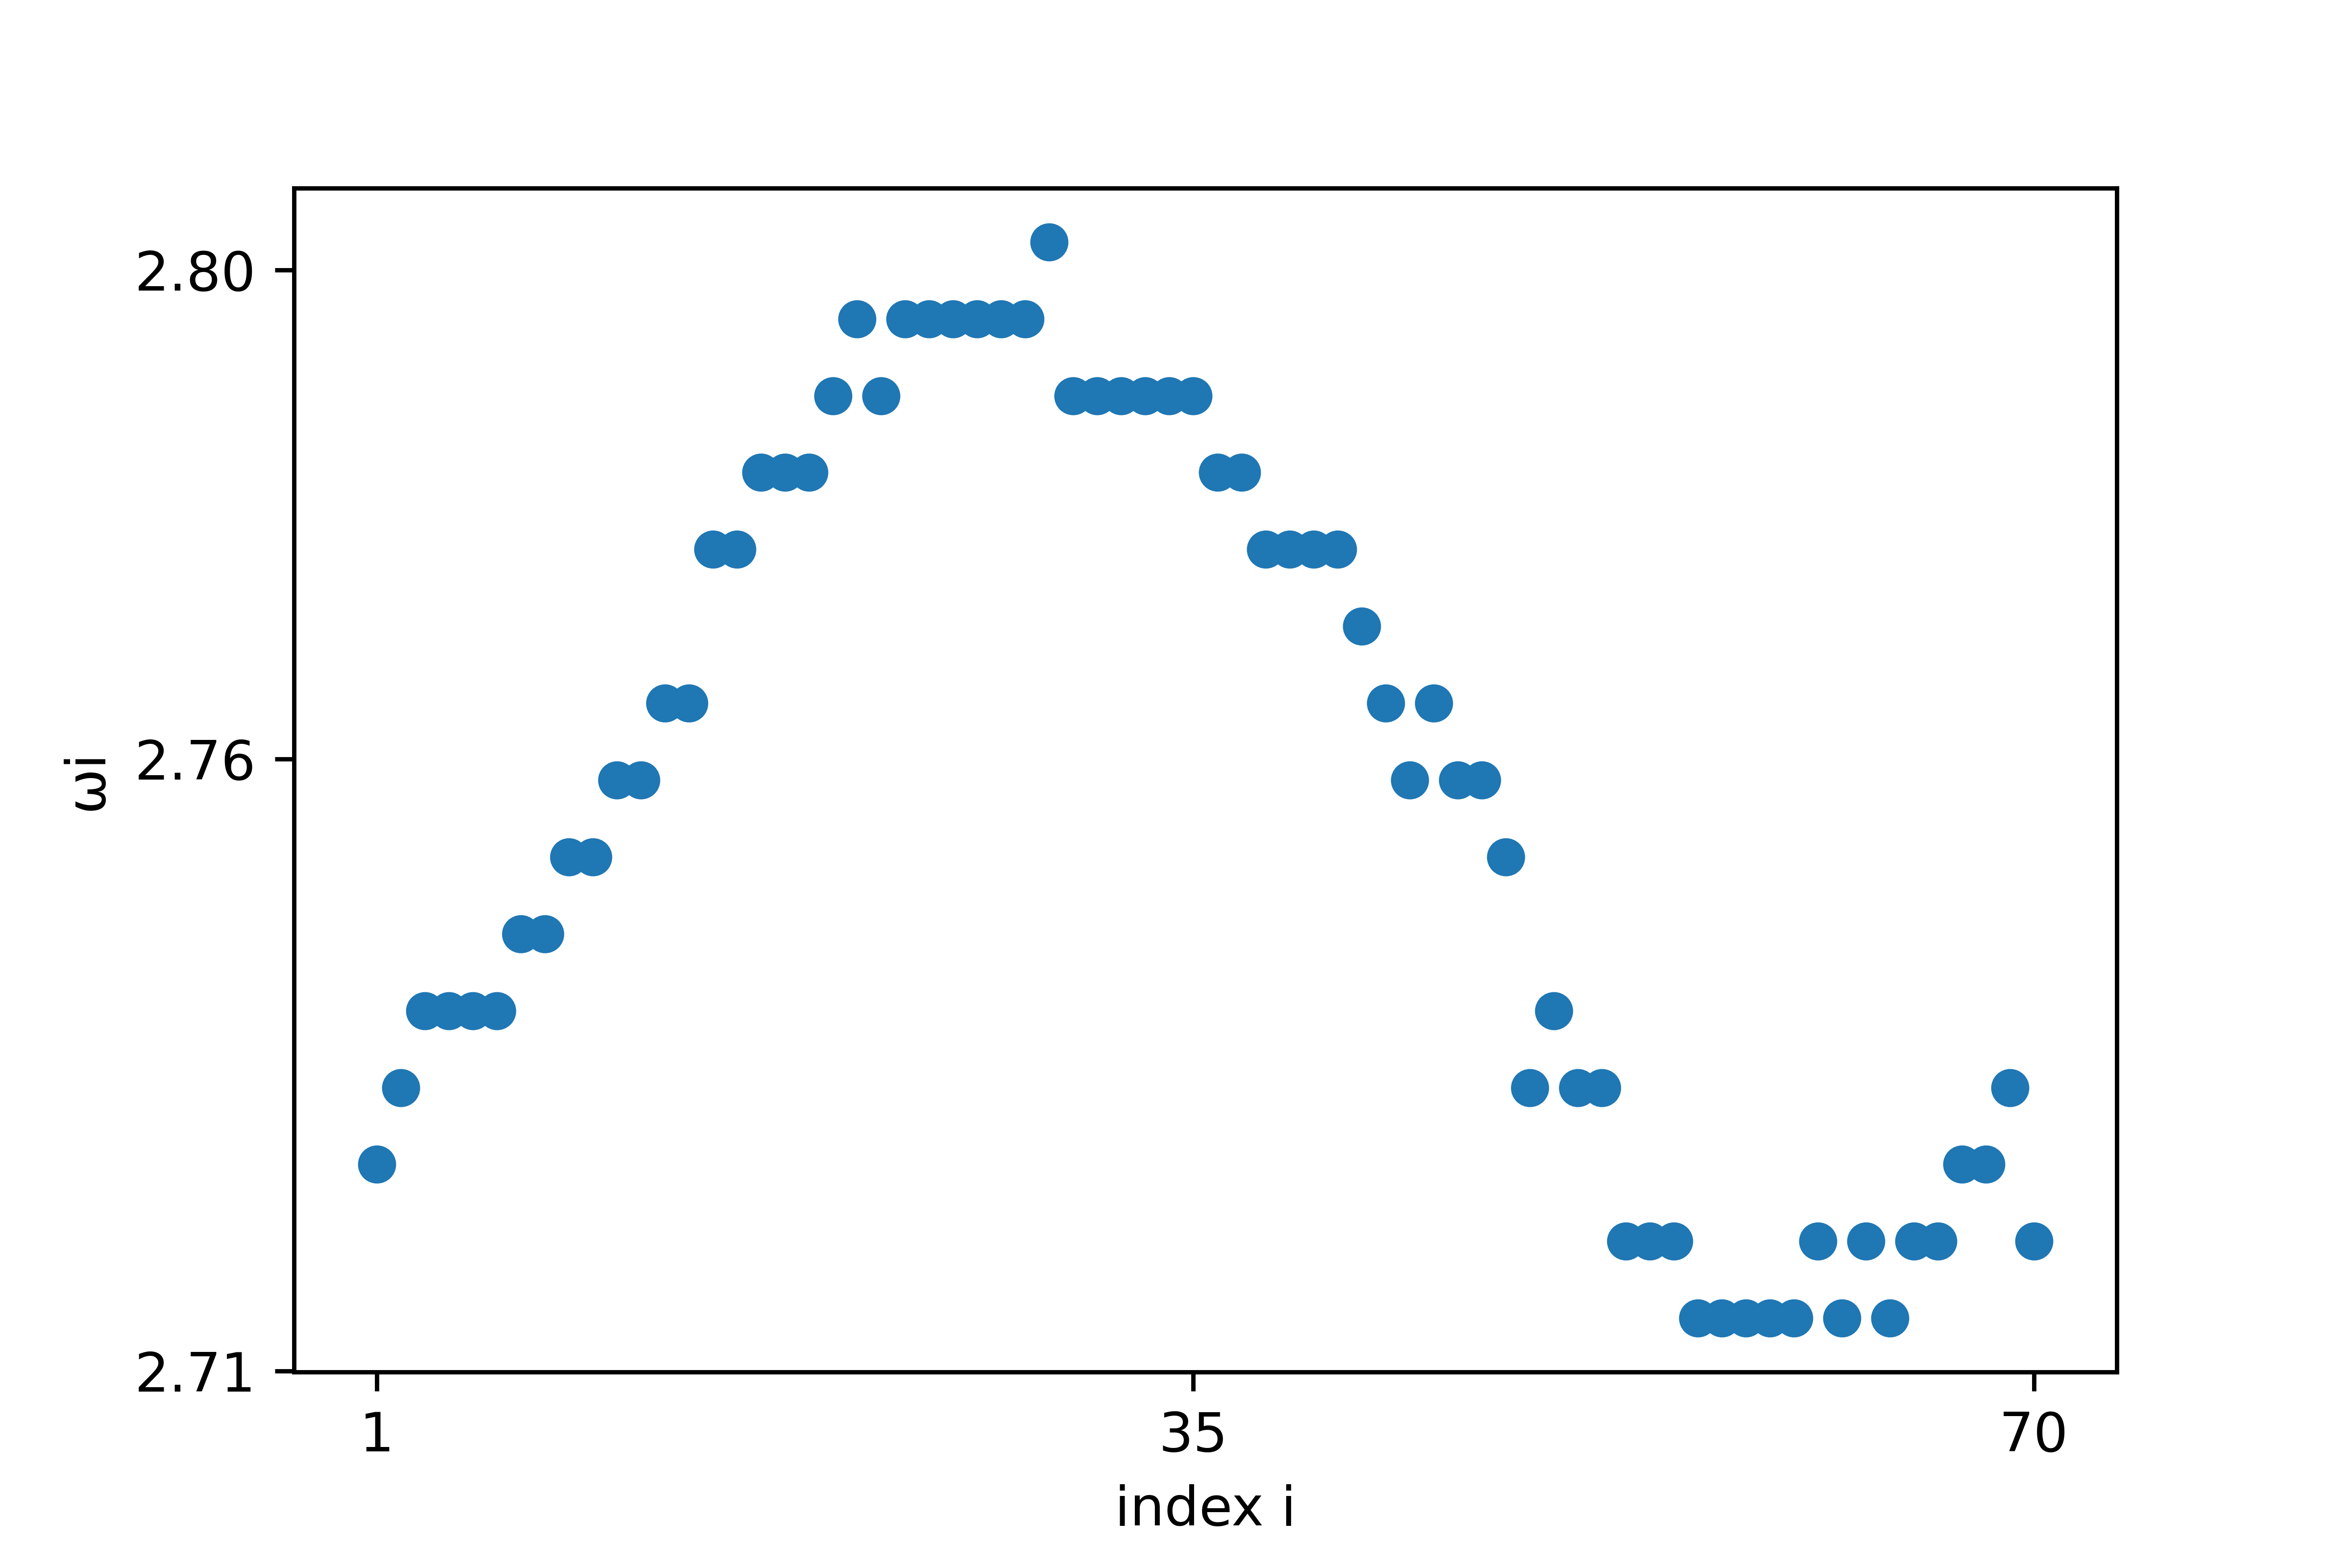
\includegraphics[width=1\linewidth]{w_N=70.png}  
  \caption{$N=70$}
\end{subfigure}
\begin{subfigure}{.32\textwidth}
  \centering
  % include first image
  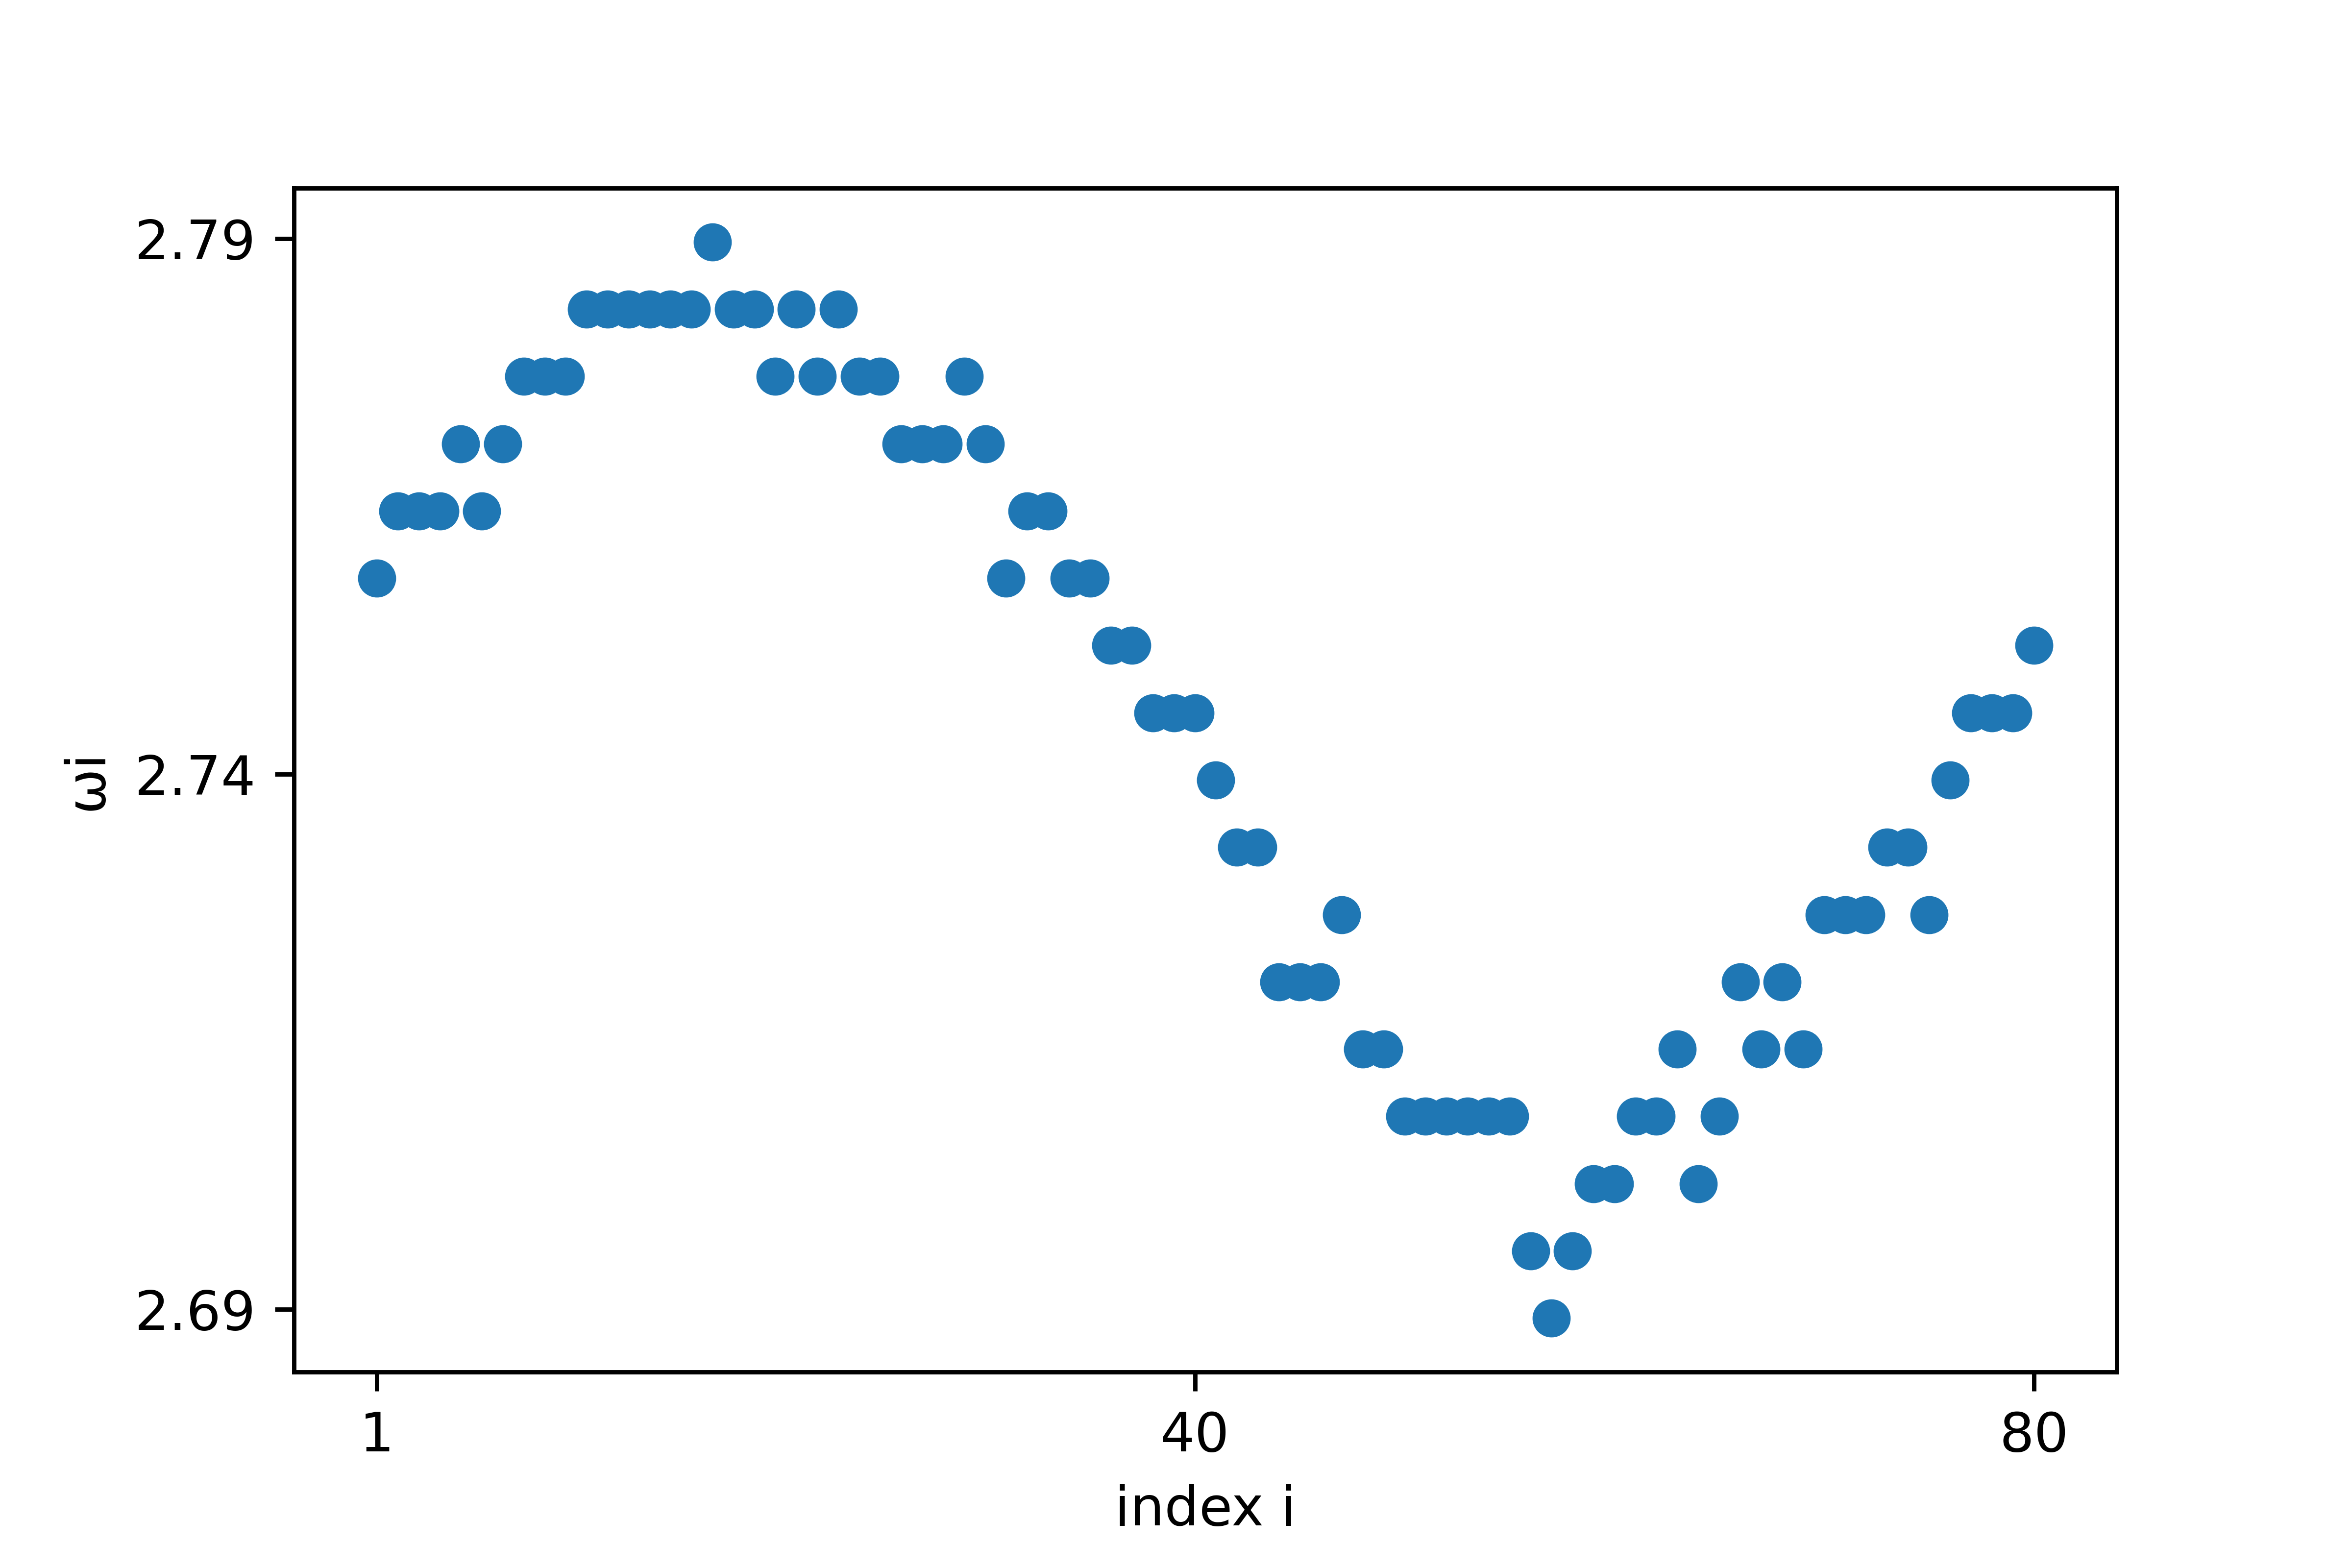
\includegraphics[width=1\linewidth]{w_N=80.png}  
  \caption{$N=80$}
\end{subfigure}
\hfill
\begin{subfigure}{.32\textwidth}
  \centering
  % include first image
  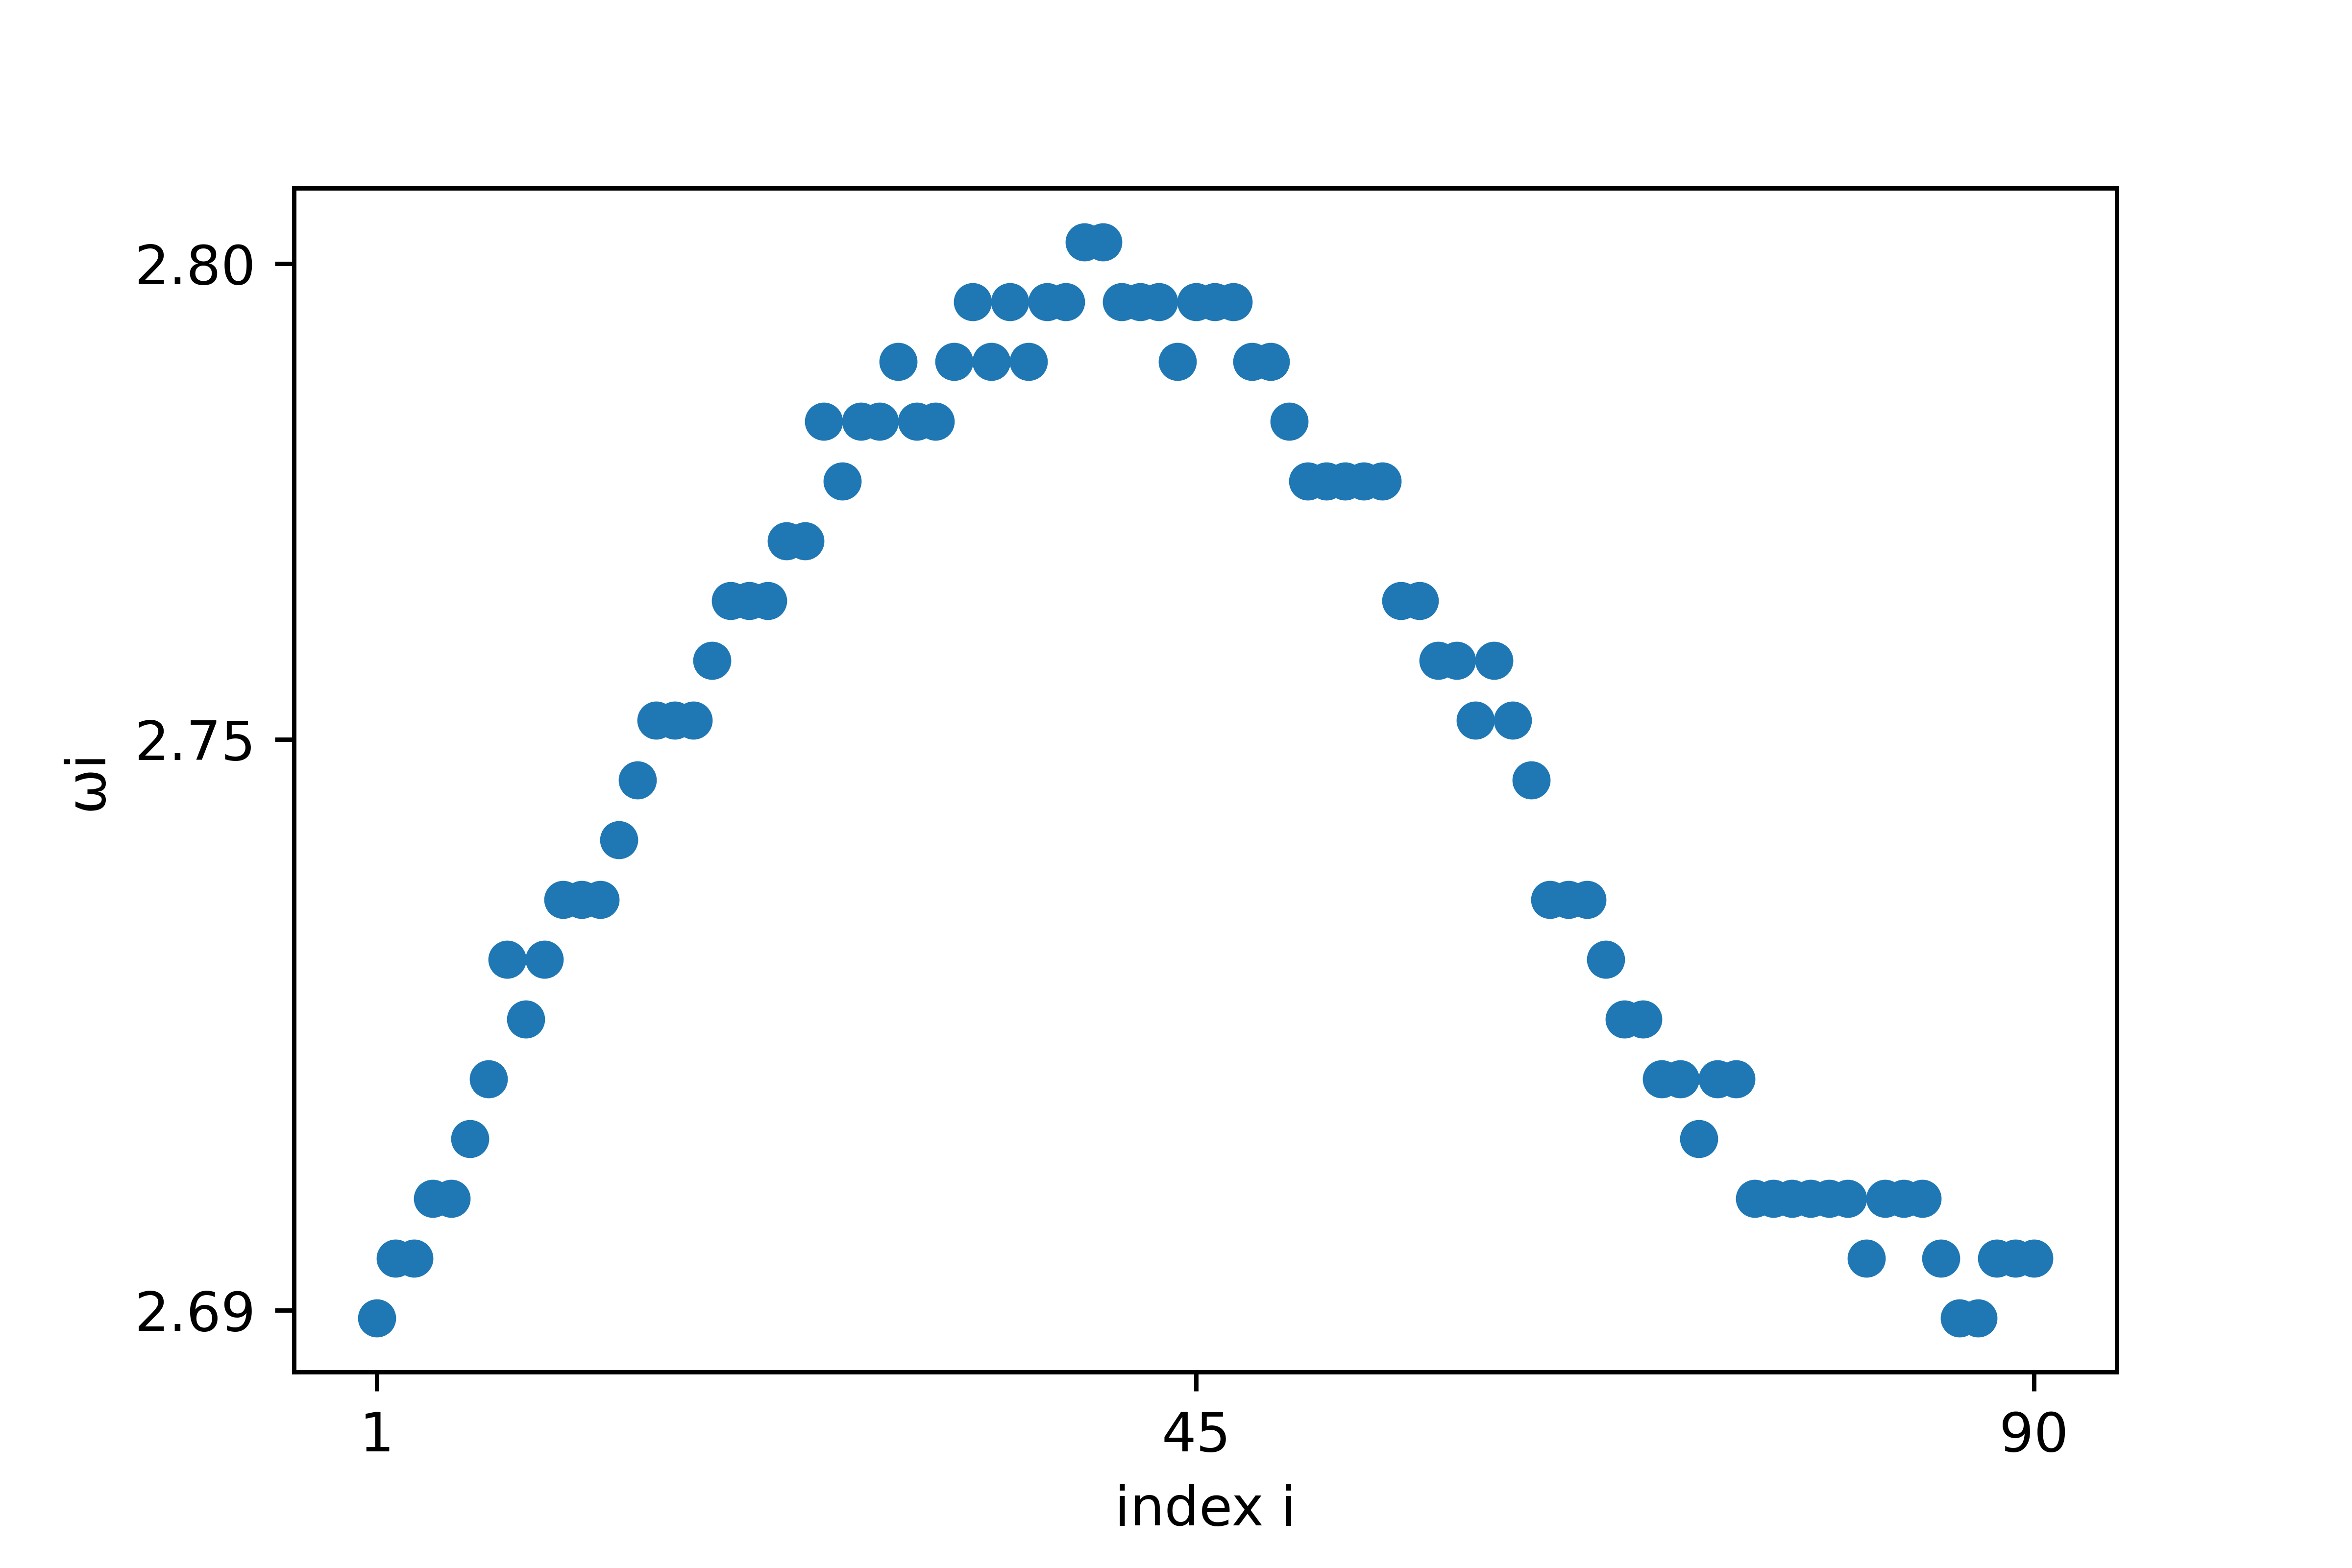
\includegraphics[width=1\linewidth]{w_N=90.png}  
  \caption{$N=90$}
\end{subfigure}
\hfill
\begin{subfigure}{.32\textwidth}
  \centering
  % include first image
  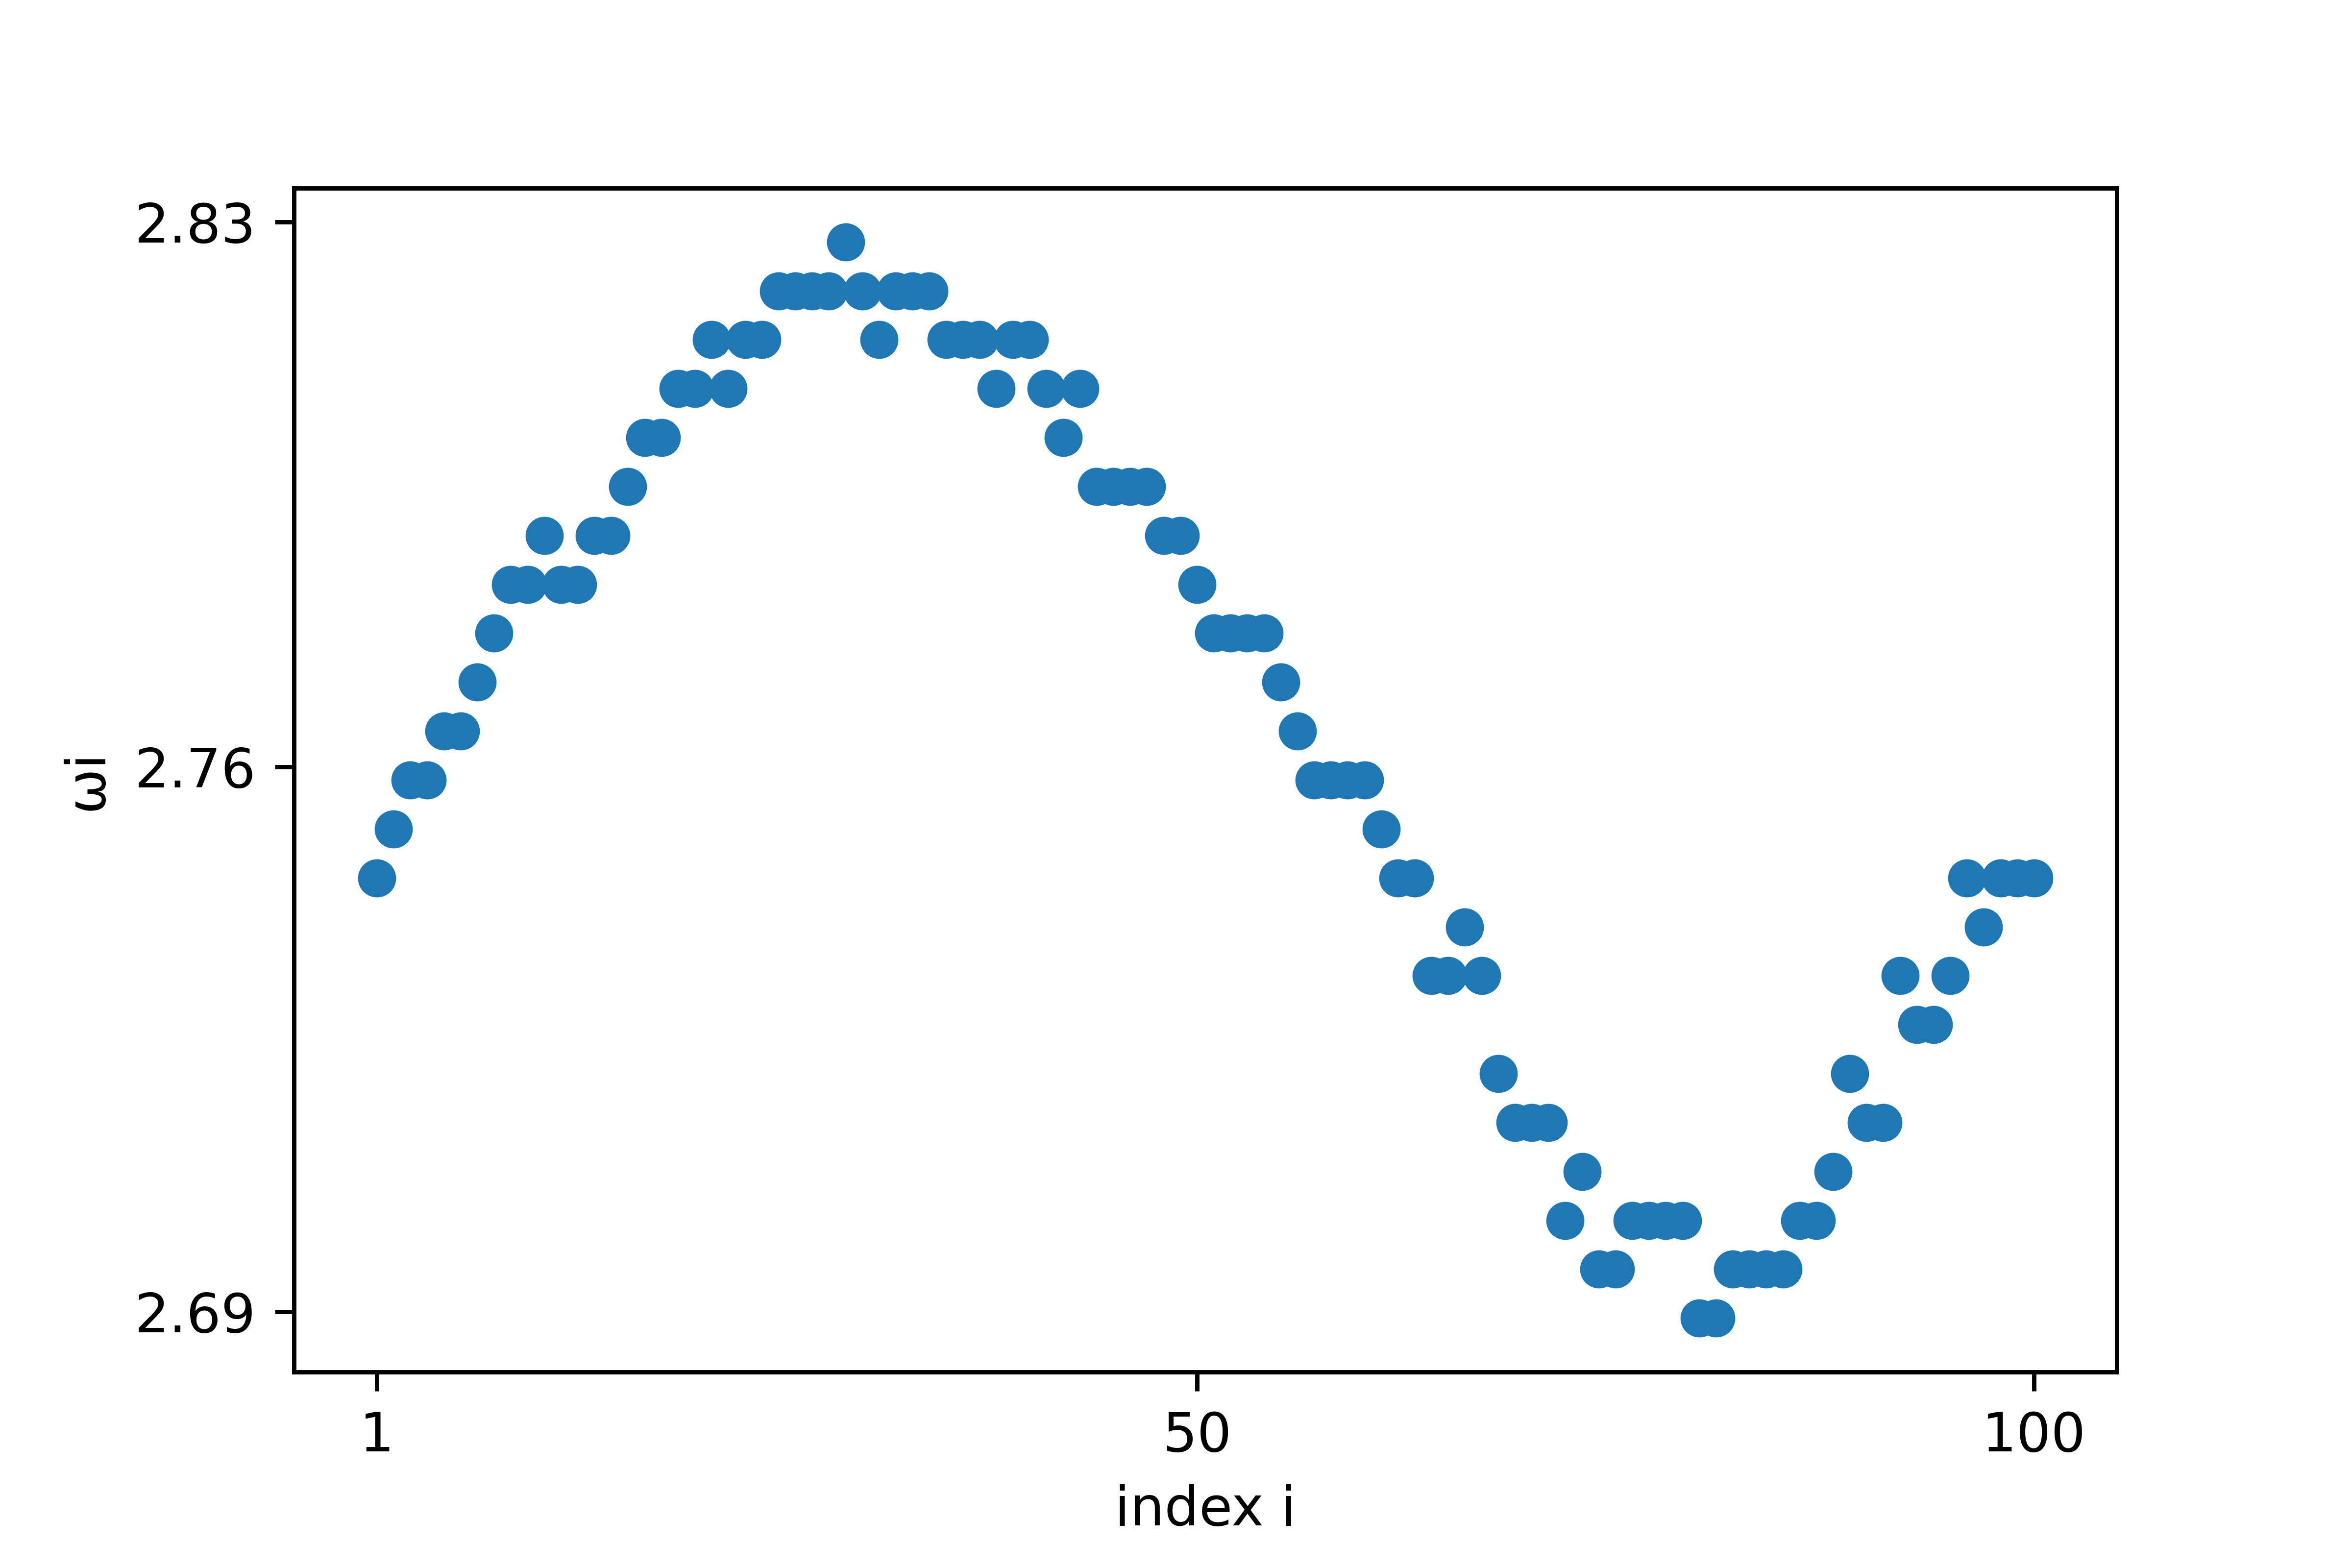
\includegraphics[width=1\linewidth]{w_N=100.png}  
  \caption{$N=100$}
\end{subfigure}
\caption{Mean phase-velocity profiles $\omega_i$ at $t=1000$ time units, for $\sigma = 0.7$, $r=0.40$ and for various values of $N$, as in Fig. (\ref{vsN}).}
\label{vsN2}
\end{figure}
\noindent We can clearly see chimera states for all $N$, but the smallest value of $N$ for which the $\omega_i$ curve is smooth enough is for $N=70$. Also, we have to compare $\Delta \omega = \omega_{\text{max}}-\omega_{\text{min}}$. In Fig. (\ref{dw}), $\Delta \omega$ vs $N$ is shown.

\begin{figure}[H]
\centering
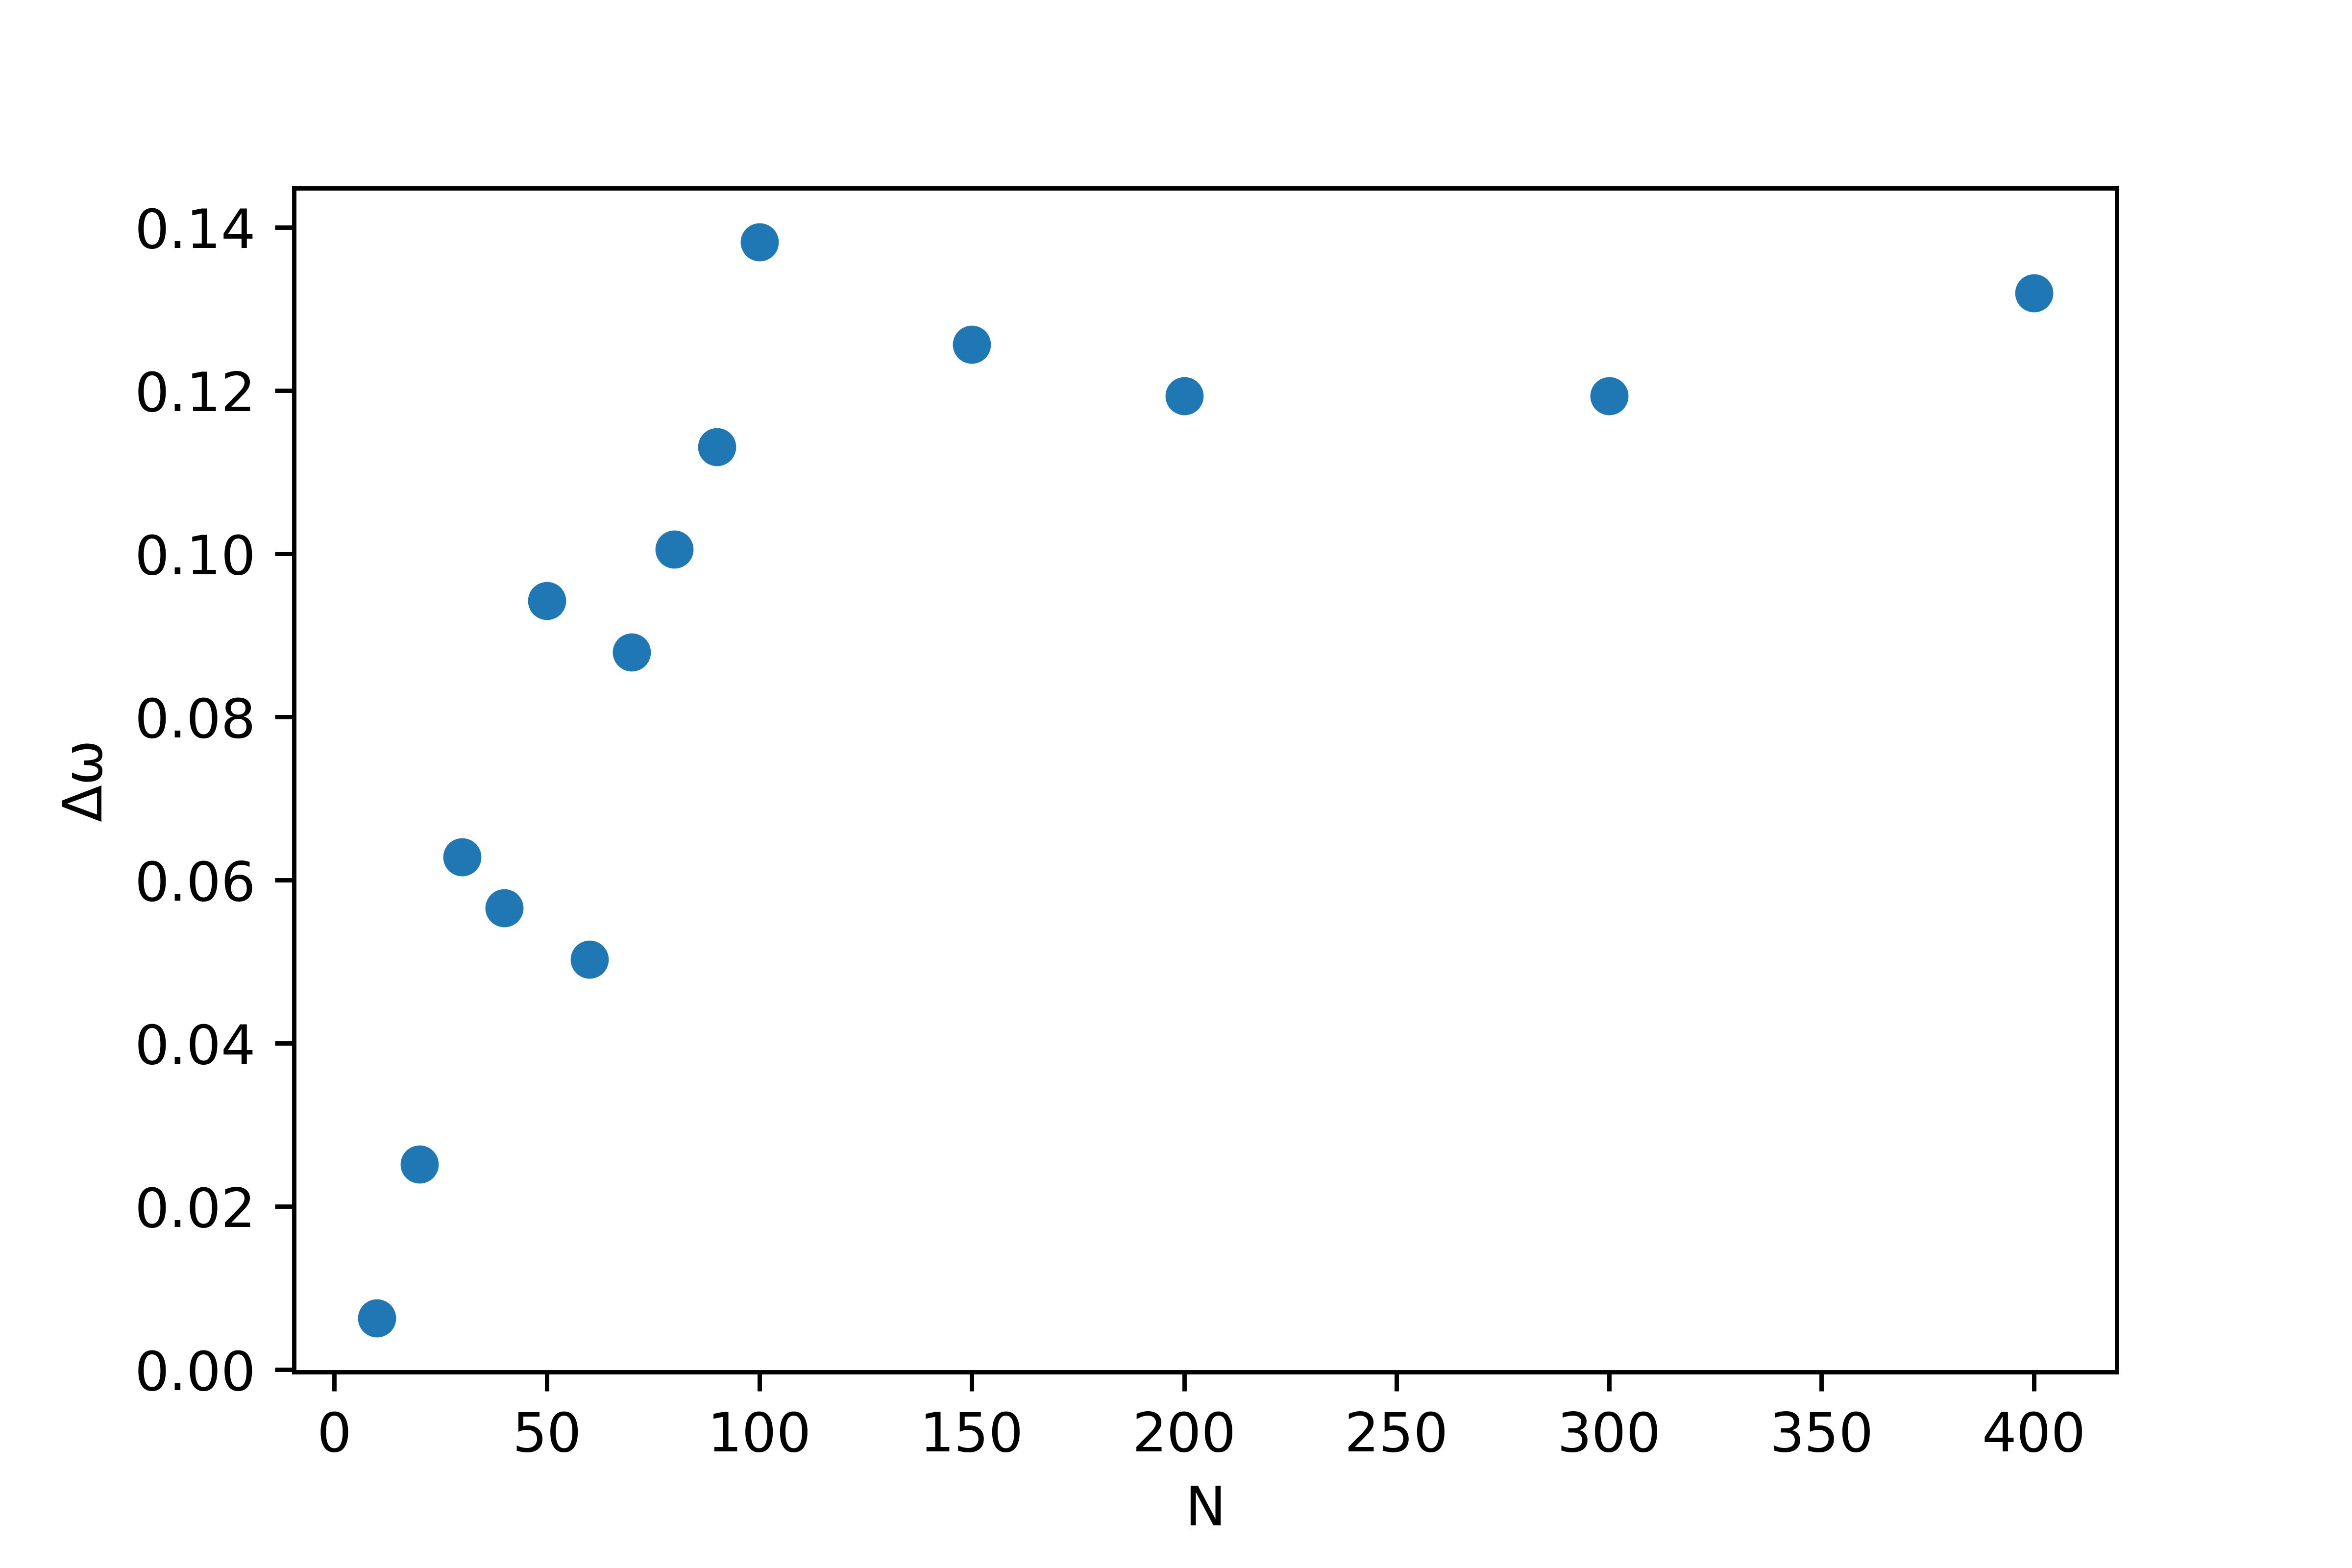
\includegraphics[width=0.6\textwidth]{deltaw_scatter.png}
\caption{$\Delta \omega = \omega_{\text{max}}-\omega_{\text{min}}$ with varying system size $N$.}
\label{dw}
\end{figure}
\noindent We conclude that the minimum number to use is $N=70$. In other words, the computationally cheapest system is with $N=70$.

\subsection{Varying $\sigma$}
We then vary $\sigma$ for $0.1 \leq \sigma \leq 2.0$, for fixed $r=0.4$ and $N=70$. We observe chimera states around $\sigma=0.7$ as before, but also at large values of $\sigma$. In particular, for $\sigma \gtrapprox 1.4$ we observe double chimeras (Fig. (\ref{dchim})). In Fig. (\ref{dchim2}), $\Delta \omega$ vs $\sigma$ is shown.

\begin{figure}[H]
\begin{subfigure}{.32\textwidth}
  \centering
  % include first image
  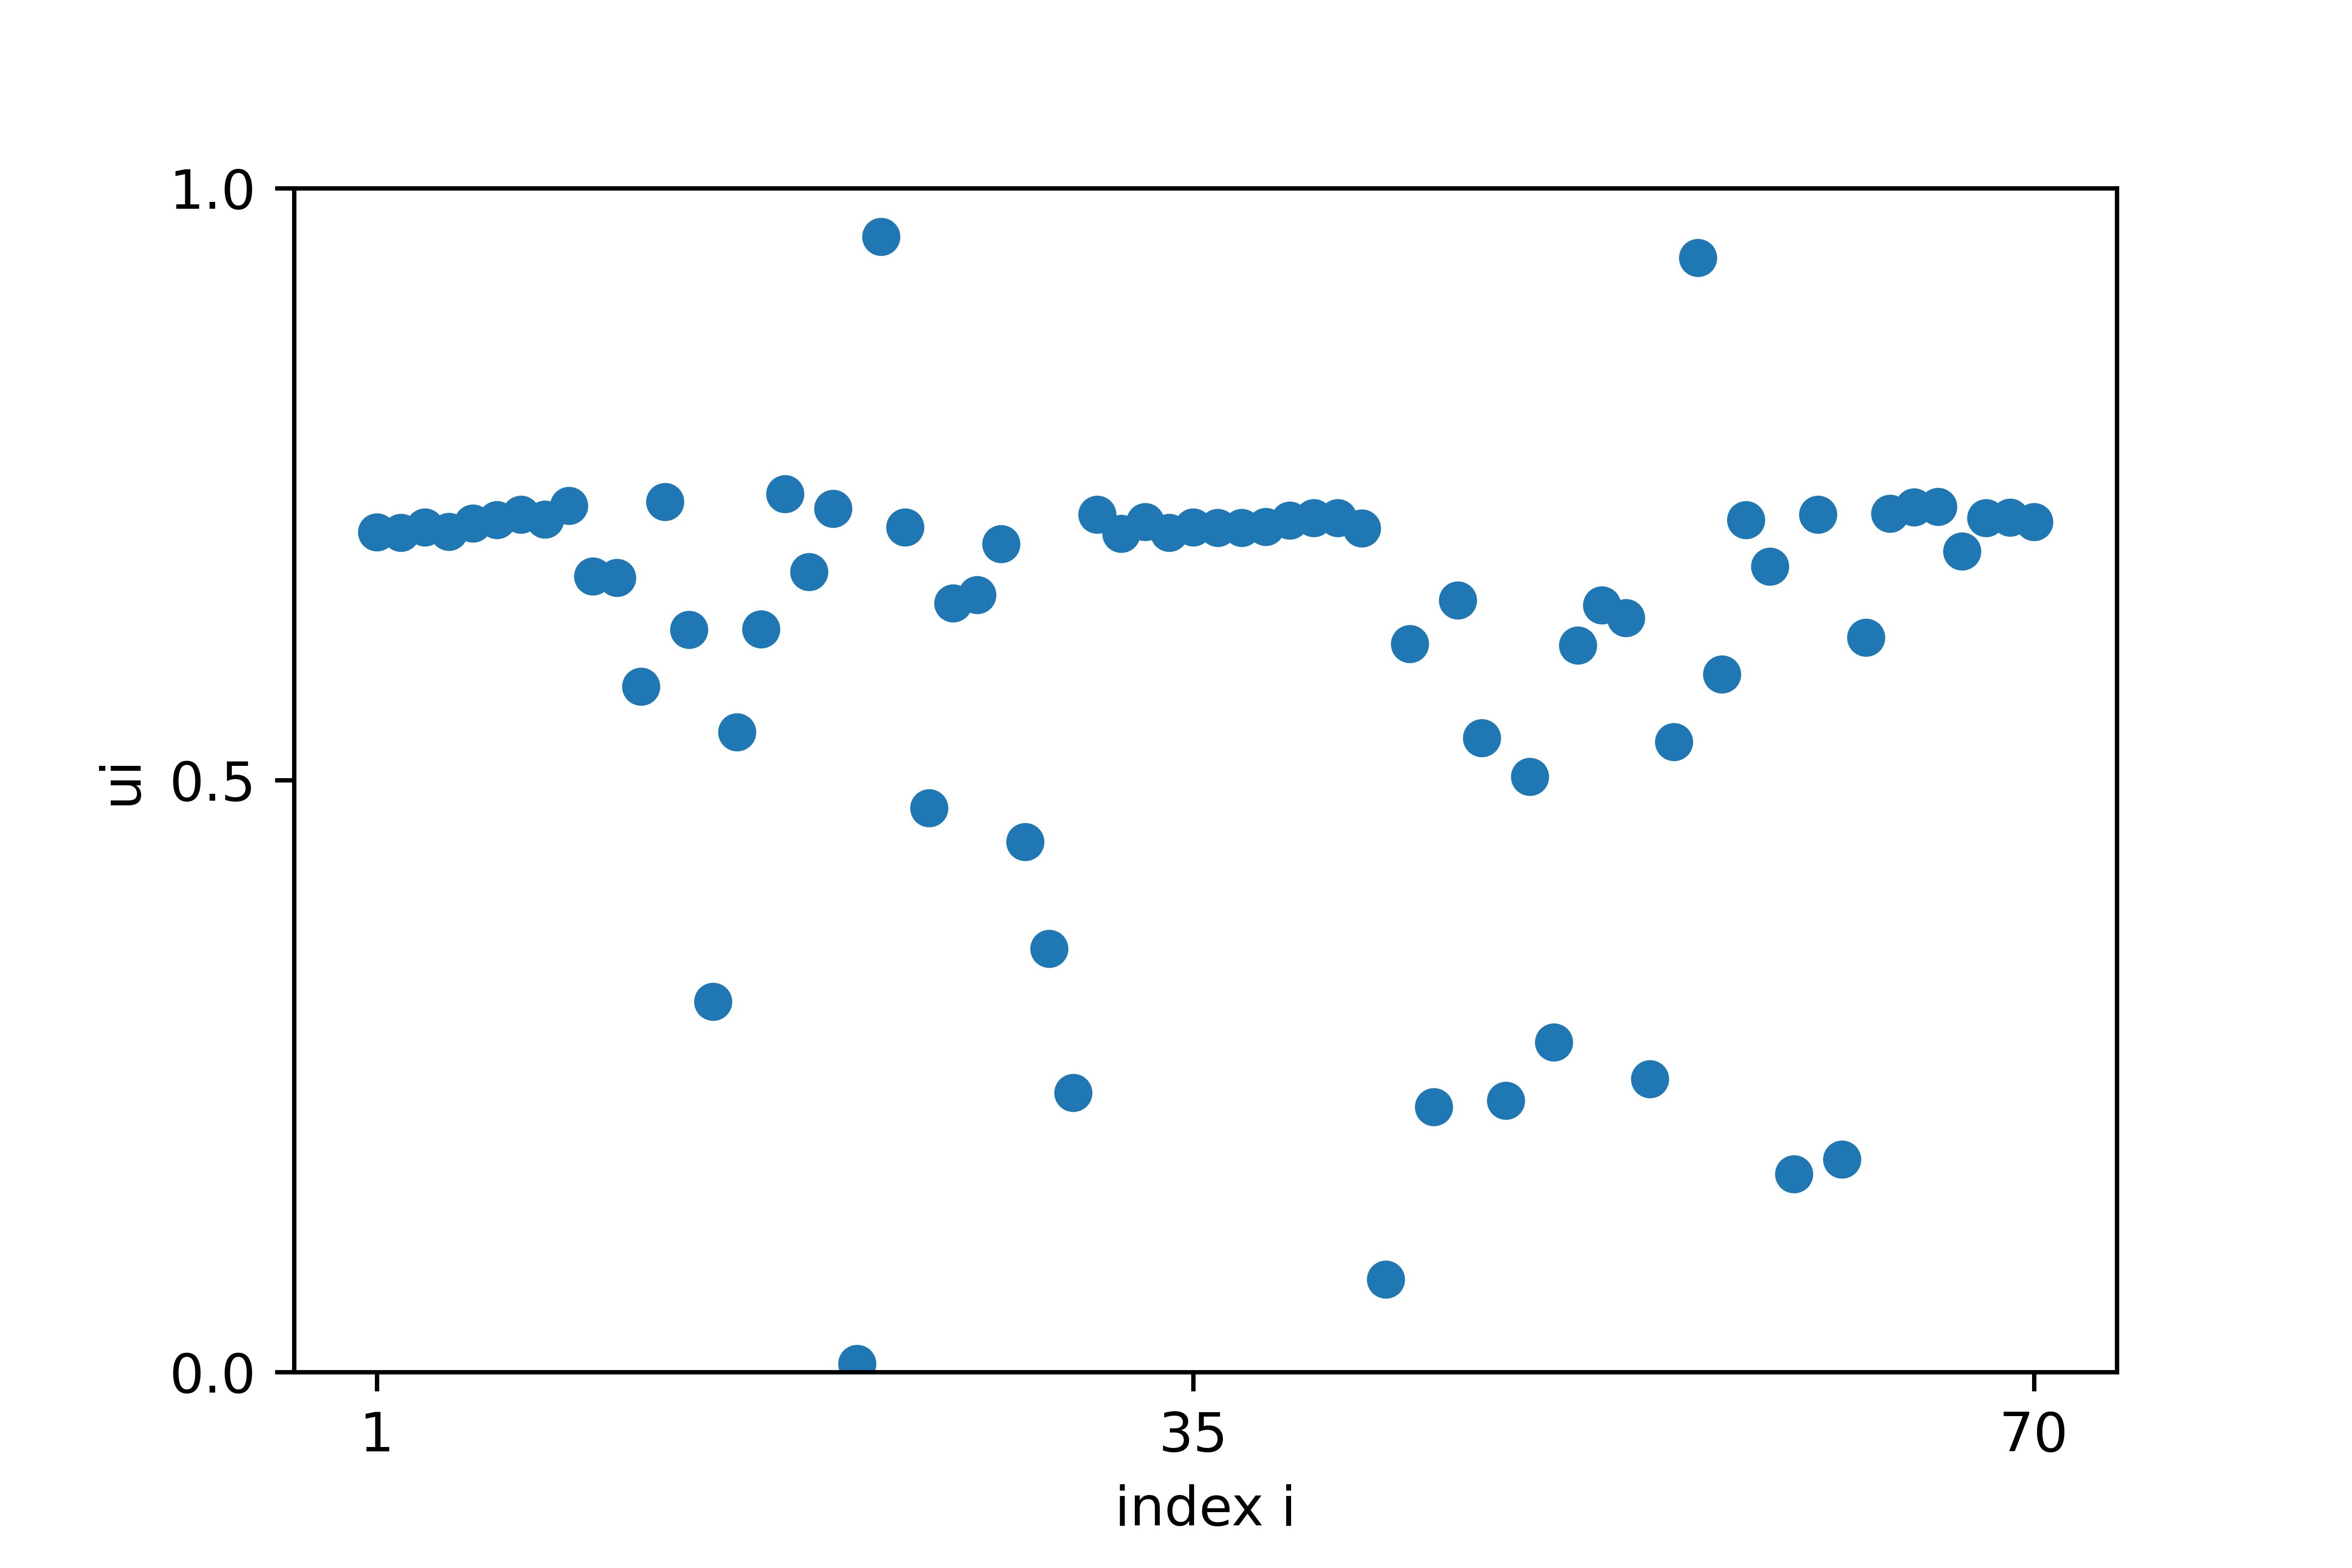
\includegraphics[width=1\linewidth]{u_sigma=1.5.png}  
  \caption{$\sigma = 1.5$}
\end{subfigure}
\hfill
\begin{subfigure}{.32\textwidth}
  \centering
  % include second image
  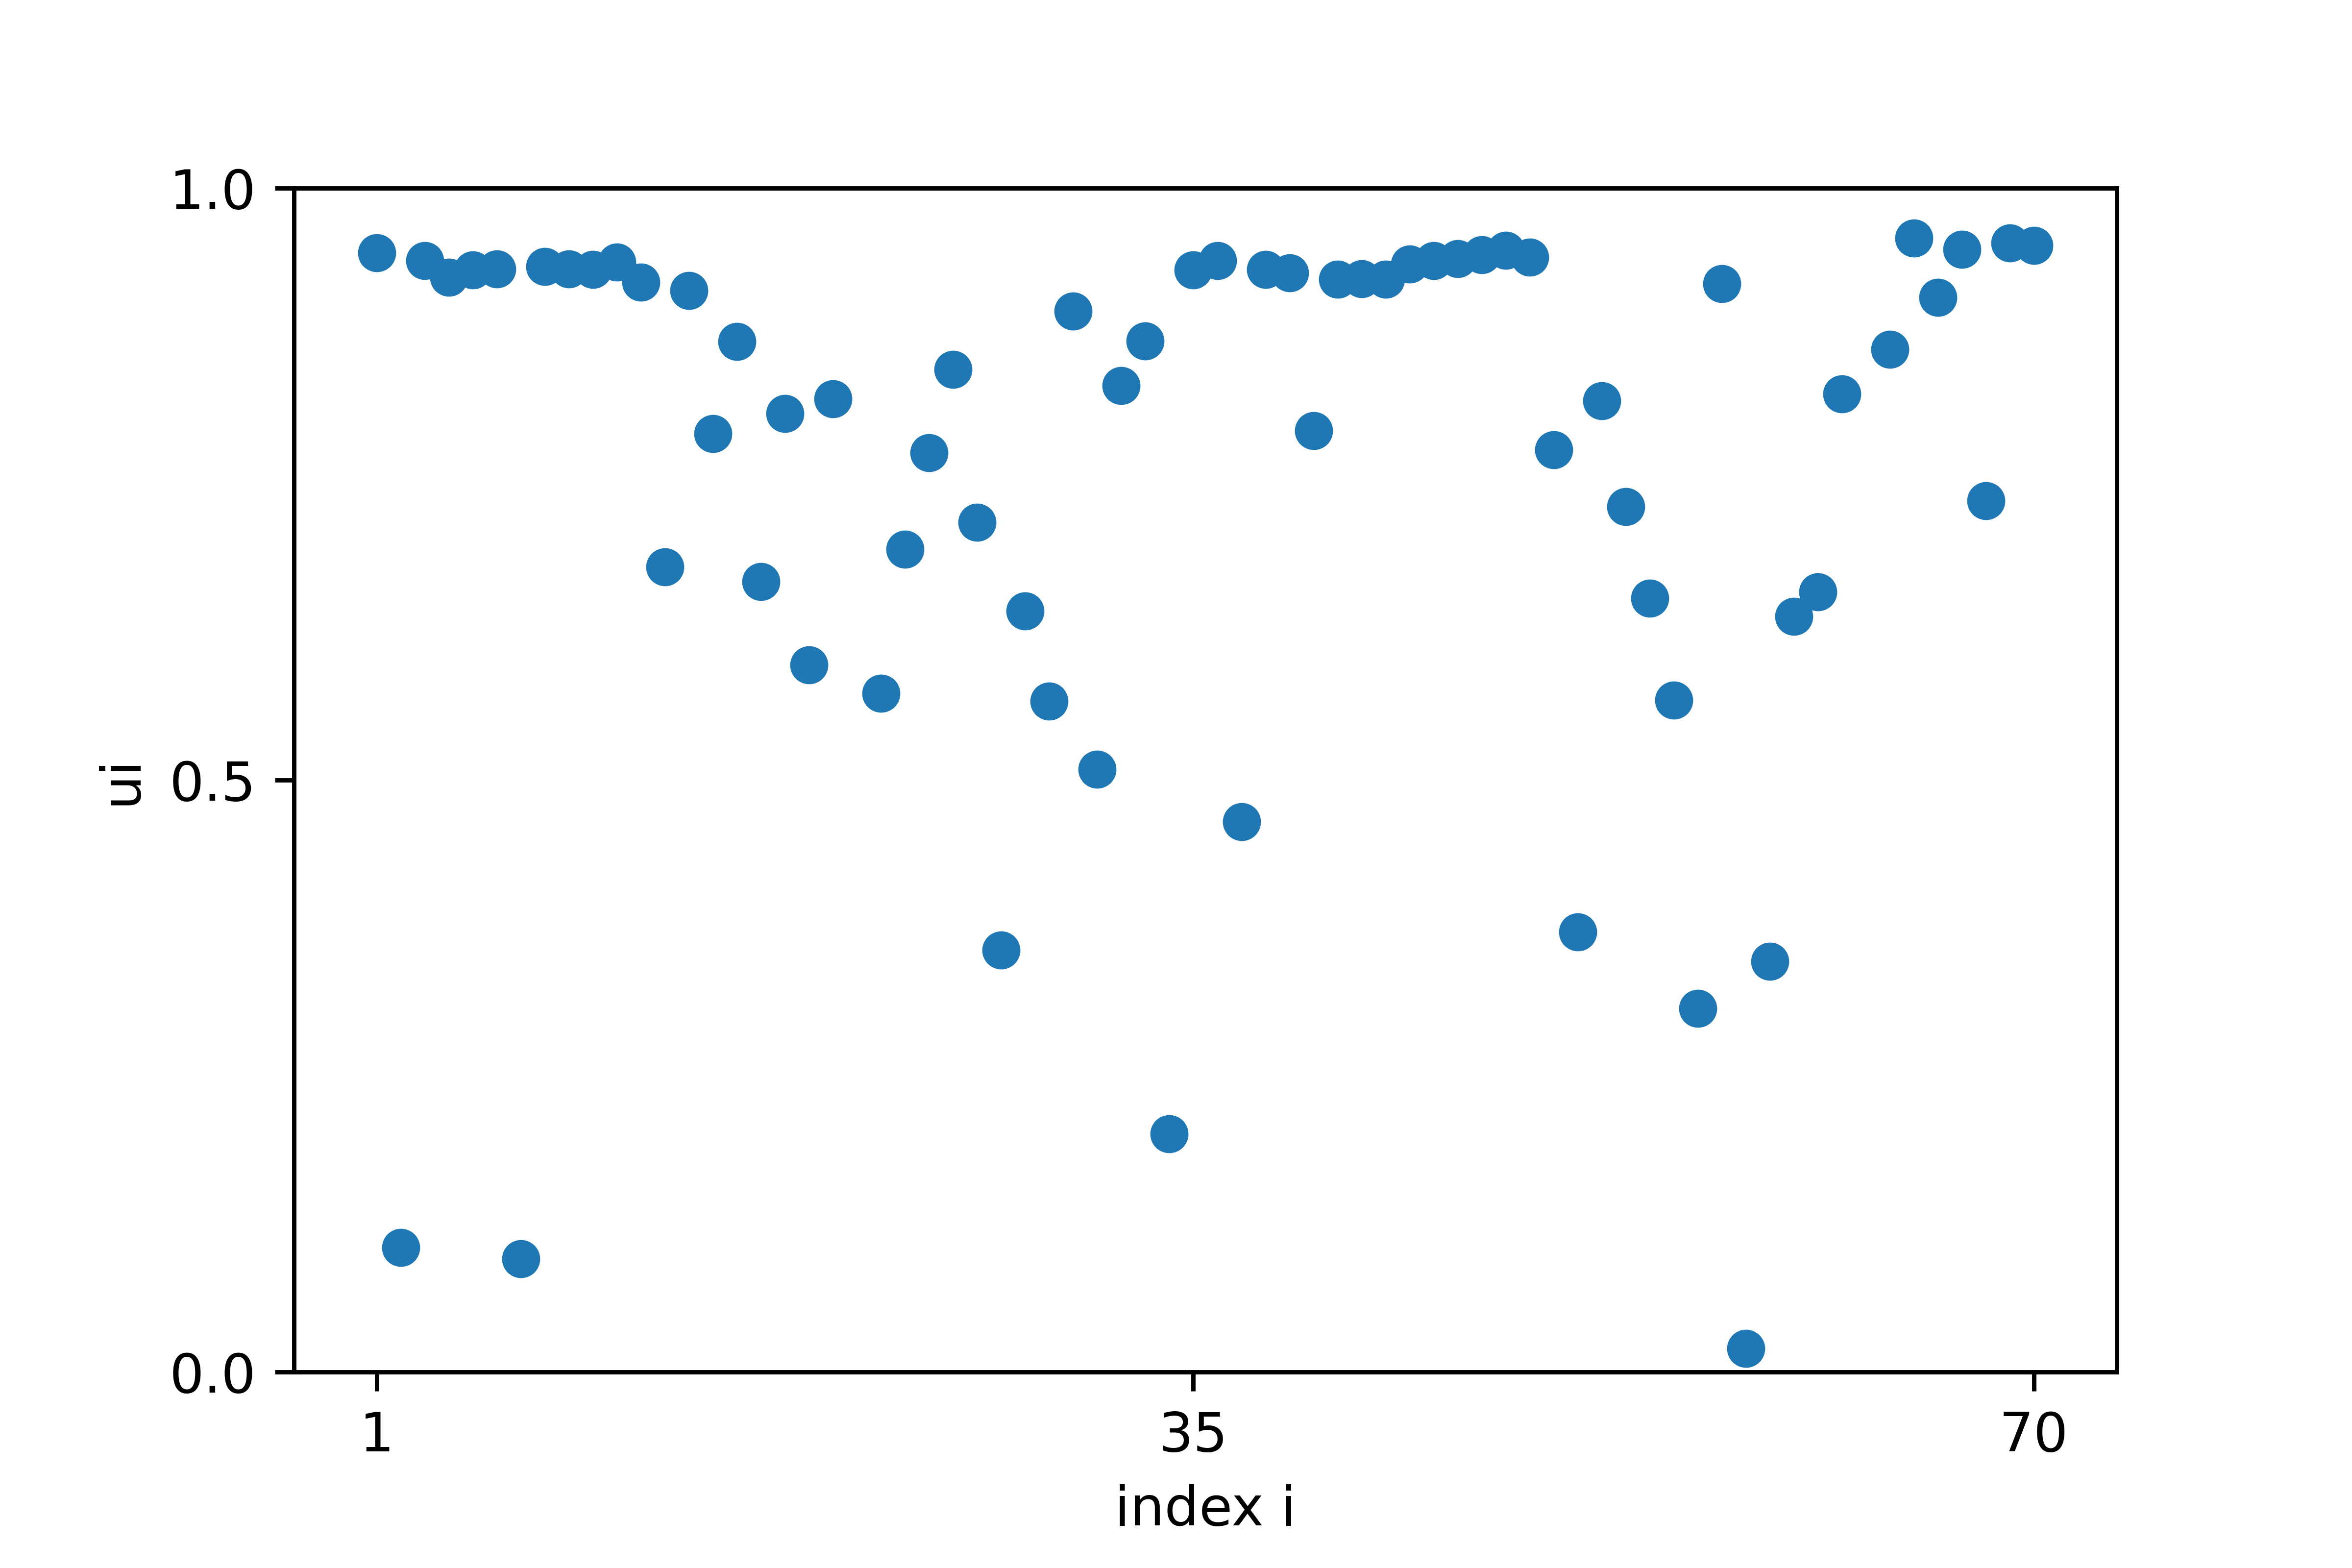
\includegraphics[width=1\linewidth]{u_sigma=1.6.png}  
  \caption{$\sigma = 1.6$}
\end{subfigure}
\hfill
\begin{subfigure}{.32\textwidth}
  \centering
  % include first image
  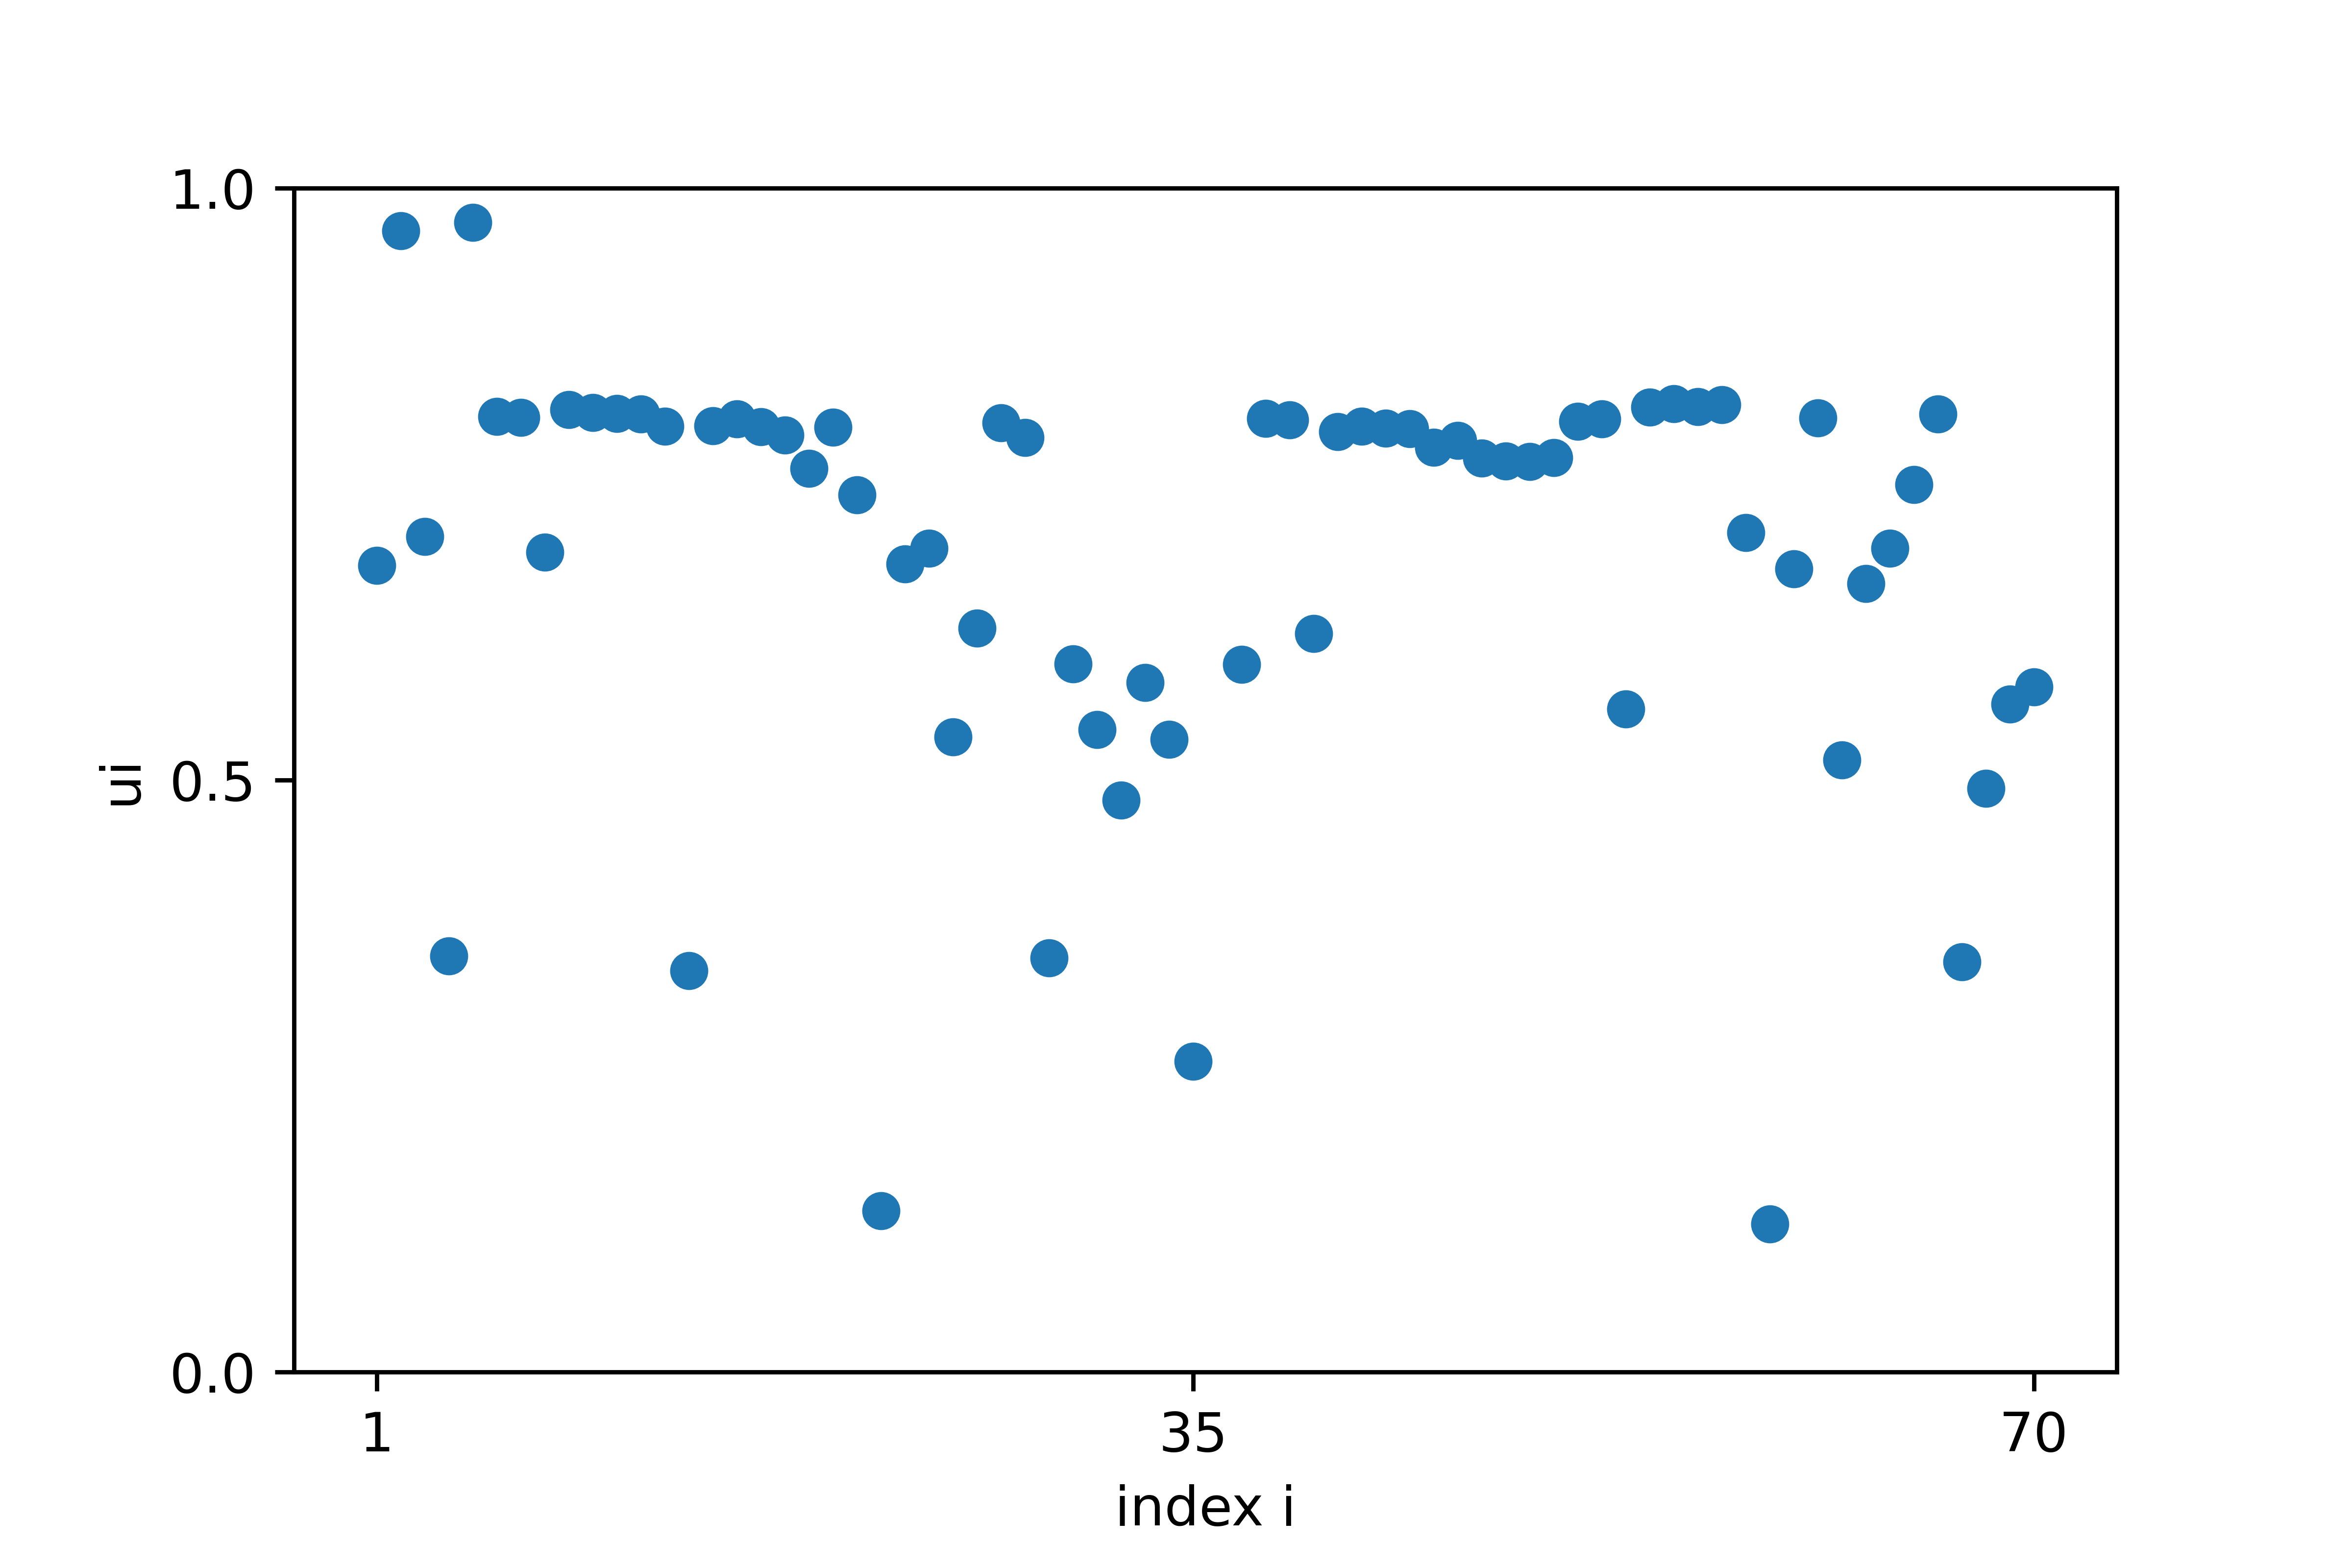
\includegraphics[width=1\linewidth]{u_sigma=1.7.png}  
  \caption{$\sigma = 1.7$}
\end{subfigure}
\begin{subfigure}{.32\textwidth}
  \centering
  % include first image
  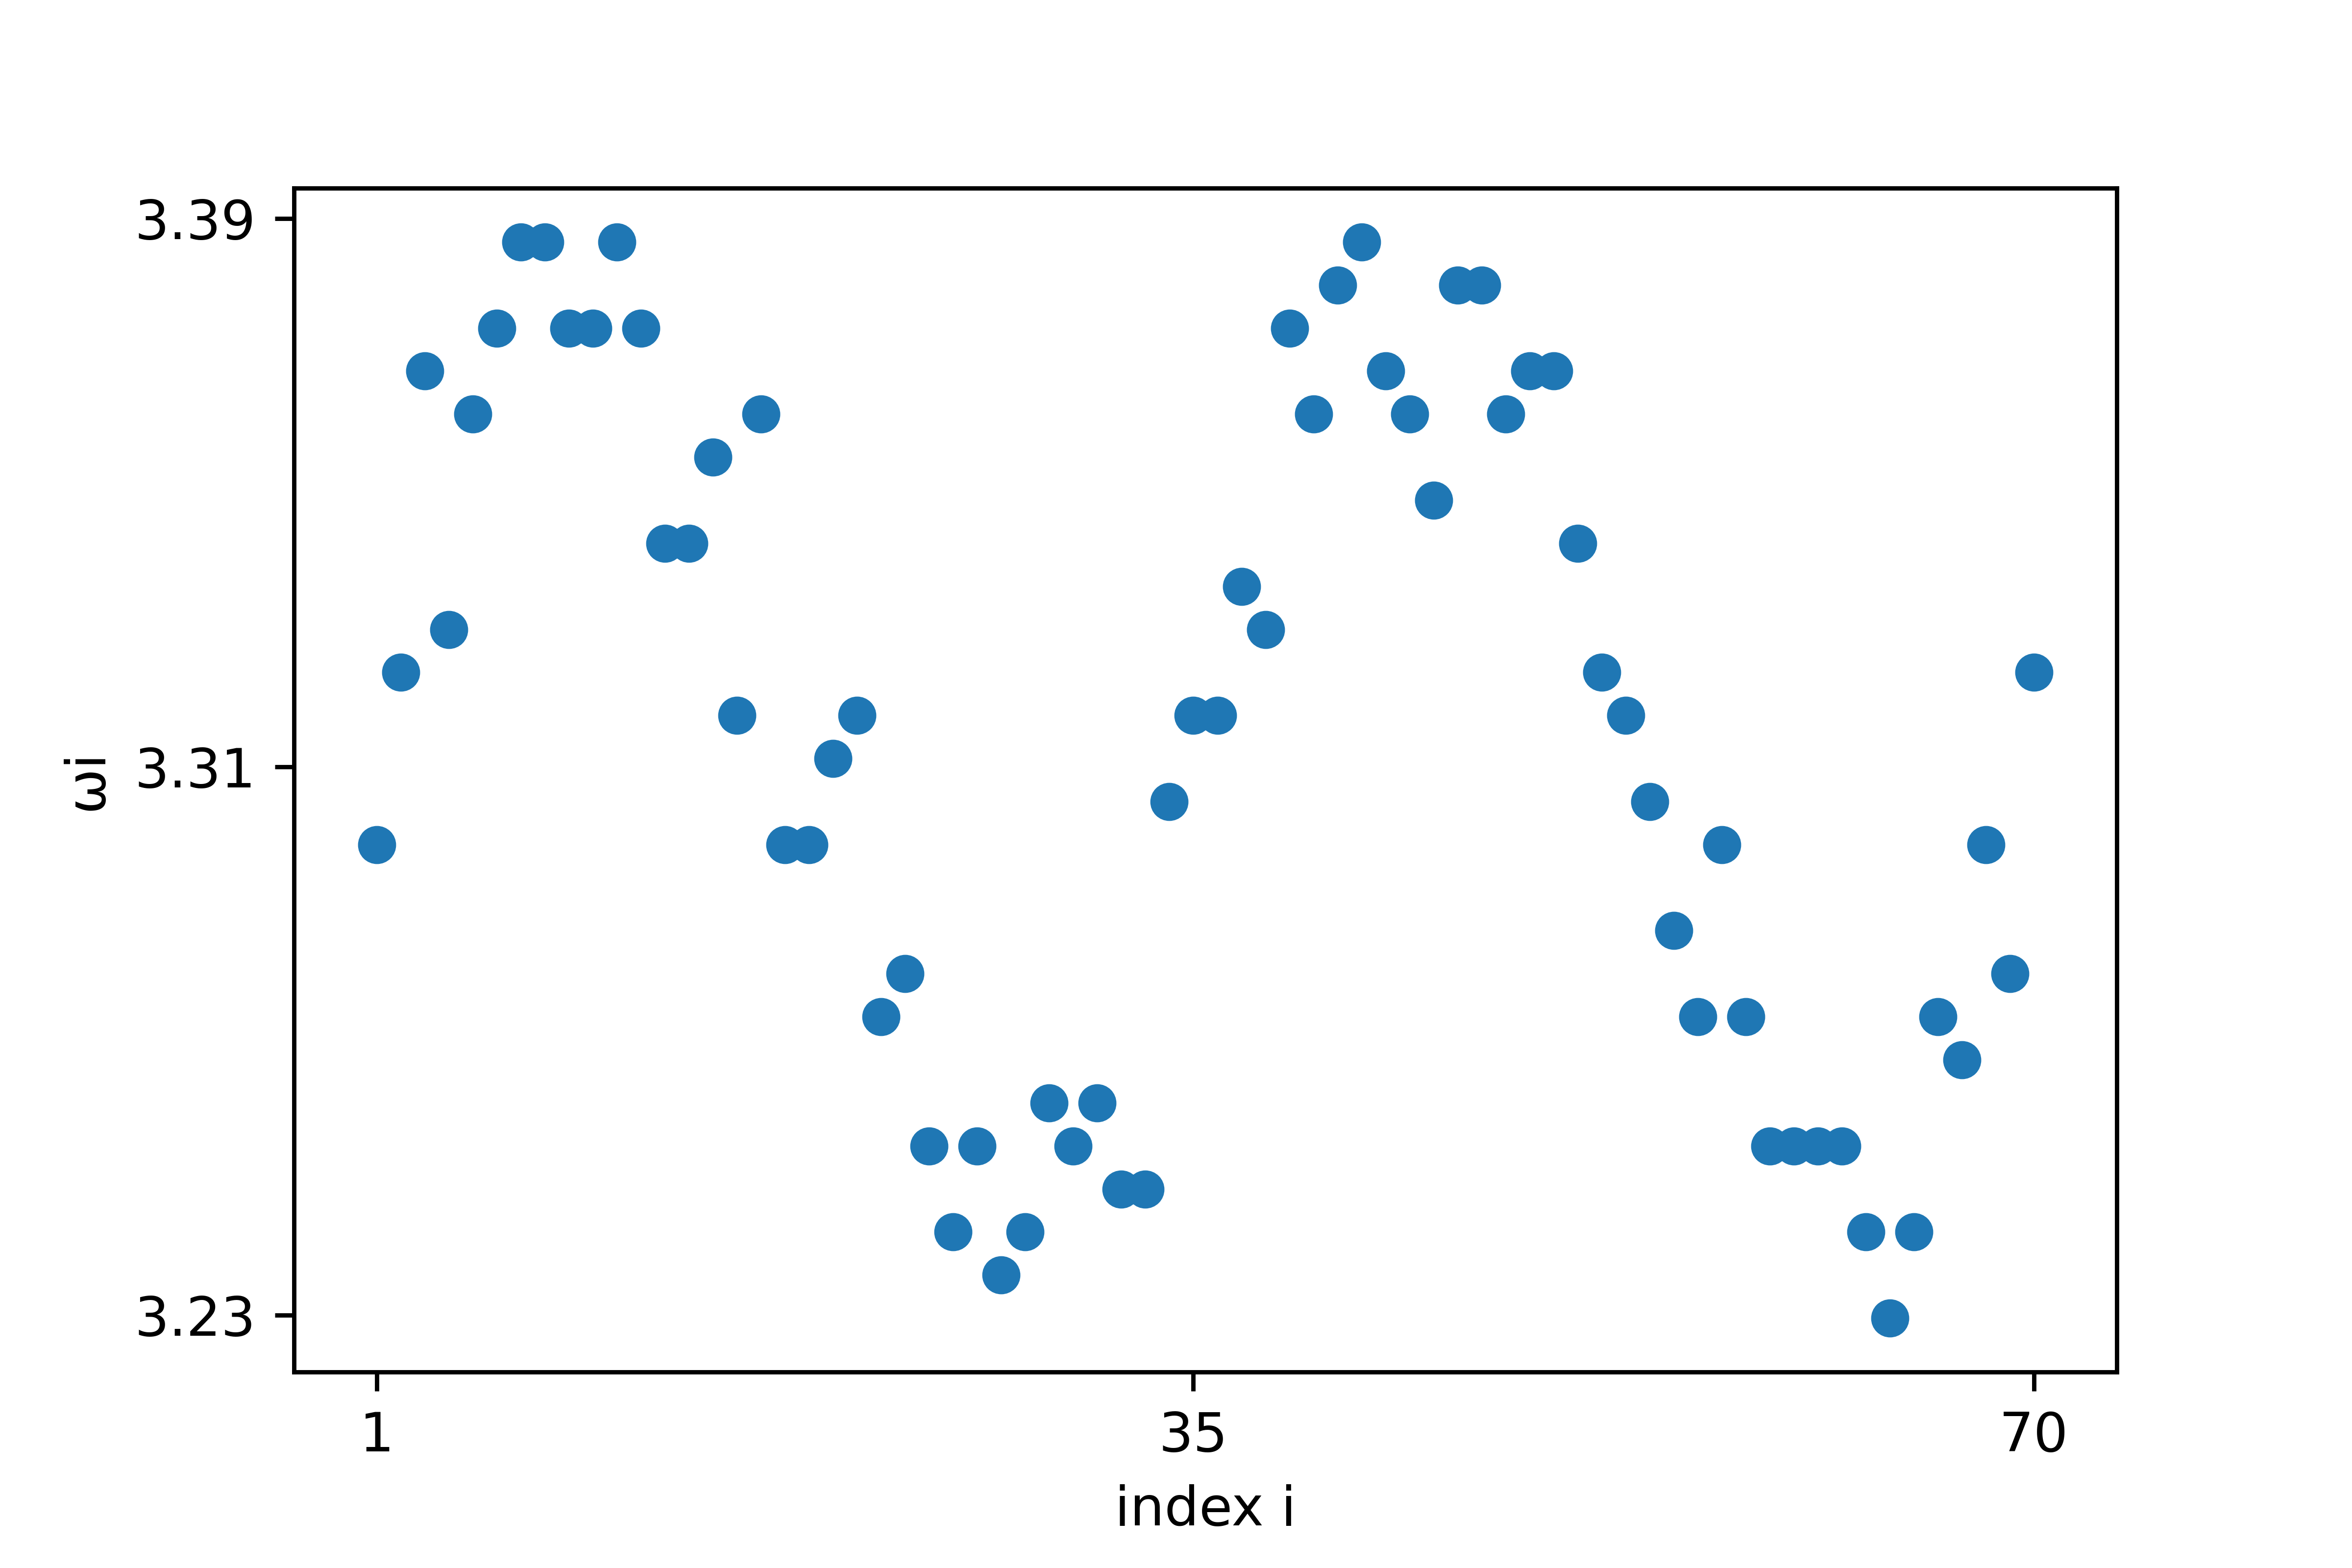
\includegraphics[width=1\linewidth]{w_sigma=1.5.png}  
  \caption{$\sigma = 1.5$}
\end{subfigure}
\hfill
\begin{subfigure}{.32\textwidth}
  \centering
  % include first image
  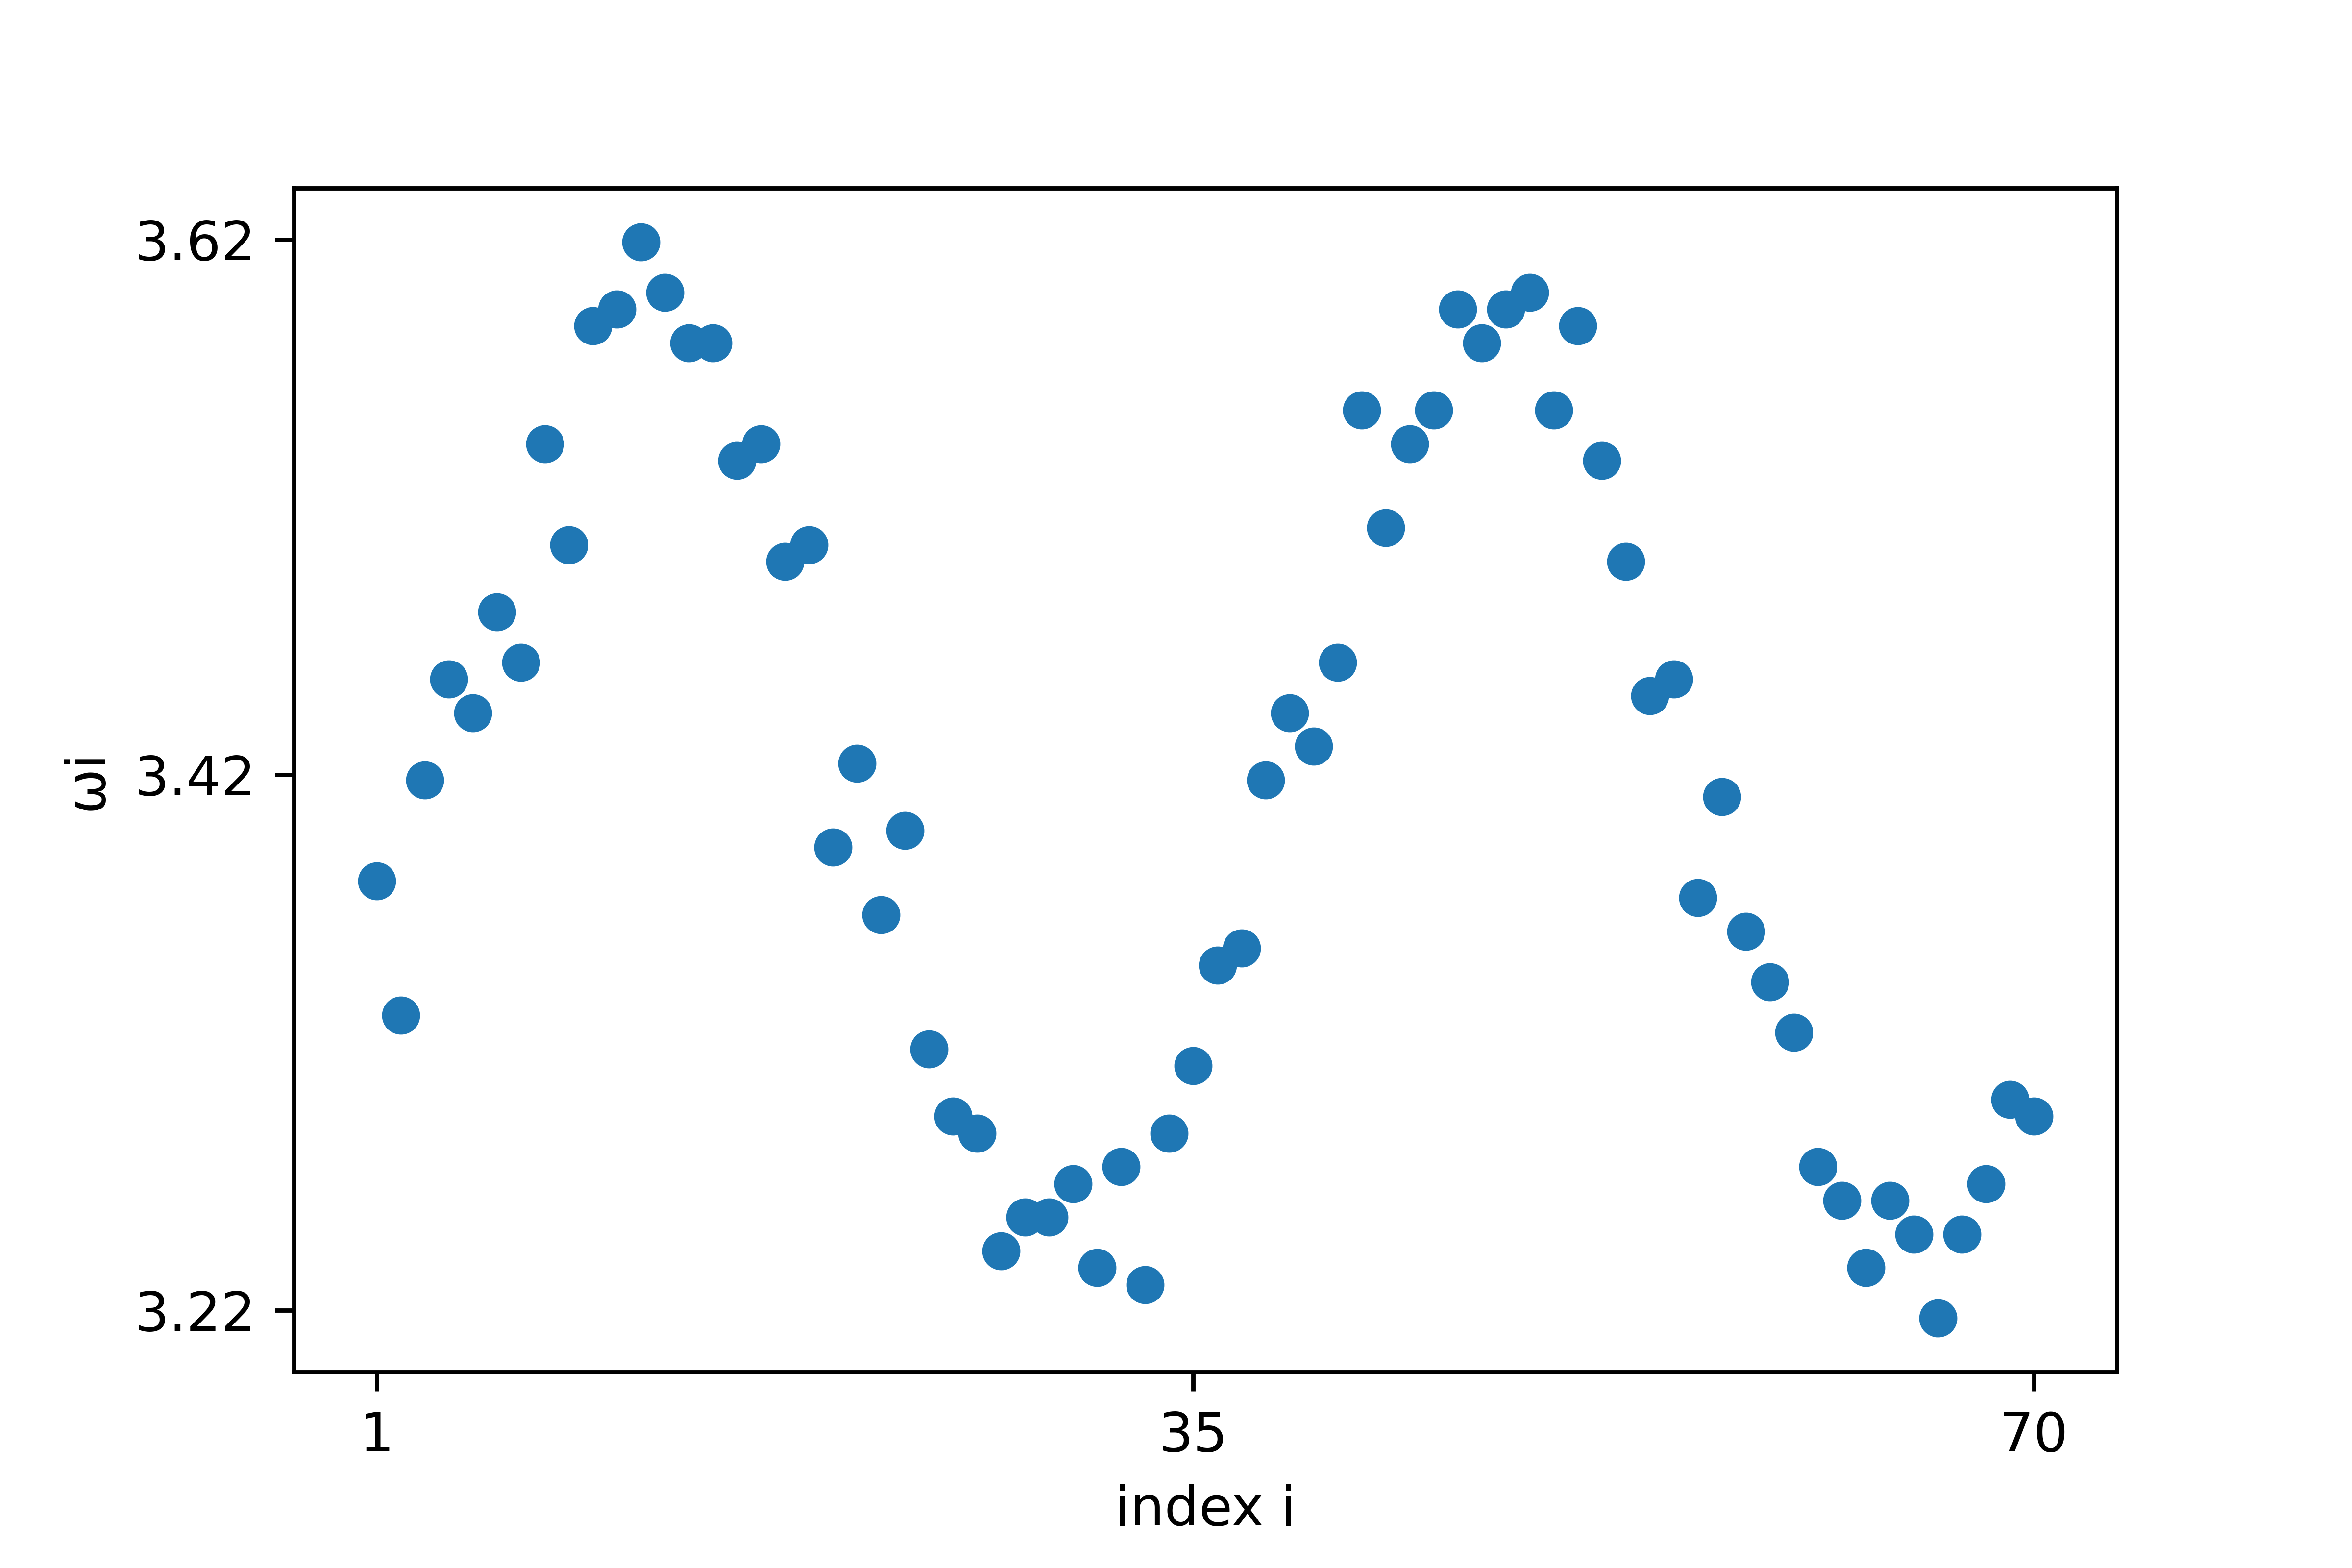
\includegraphics[width=1\linewidth]{w_sigma=1.6.png}  
  \caption{$\sigma = 1.6$}
\end{subfigure}
\hfill
\begin{subfigure}{.32\textwidth}
  \centering
  % include first image
  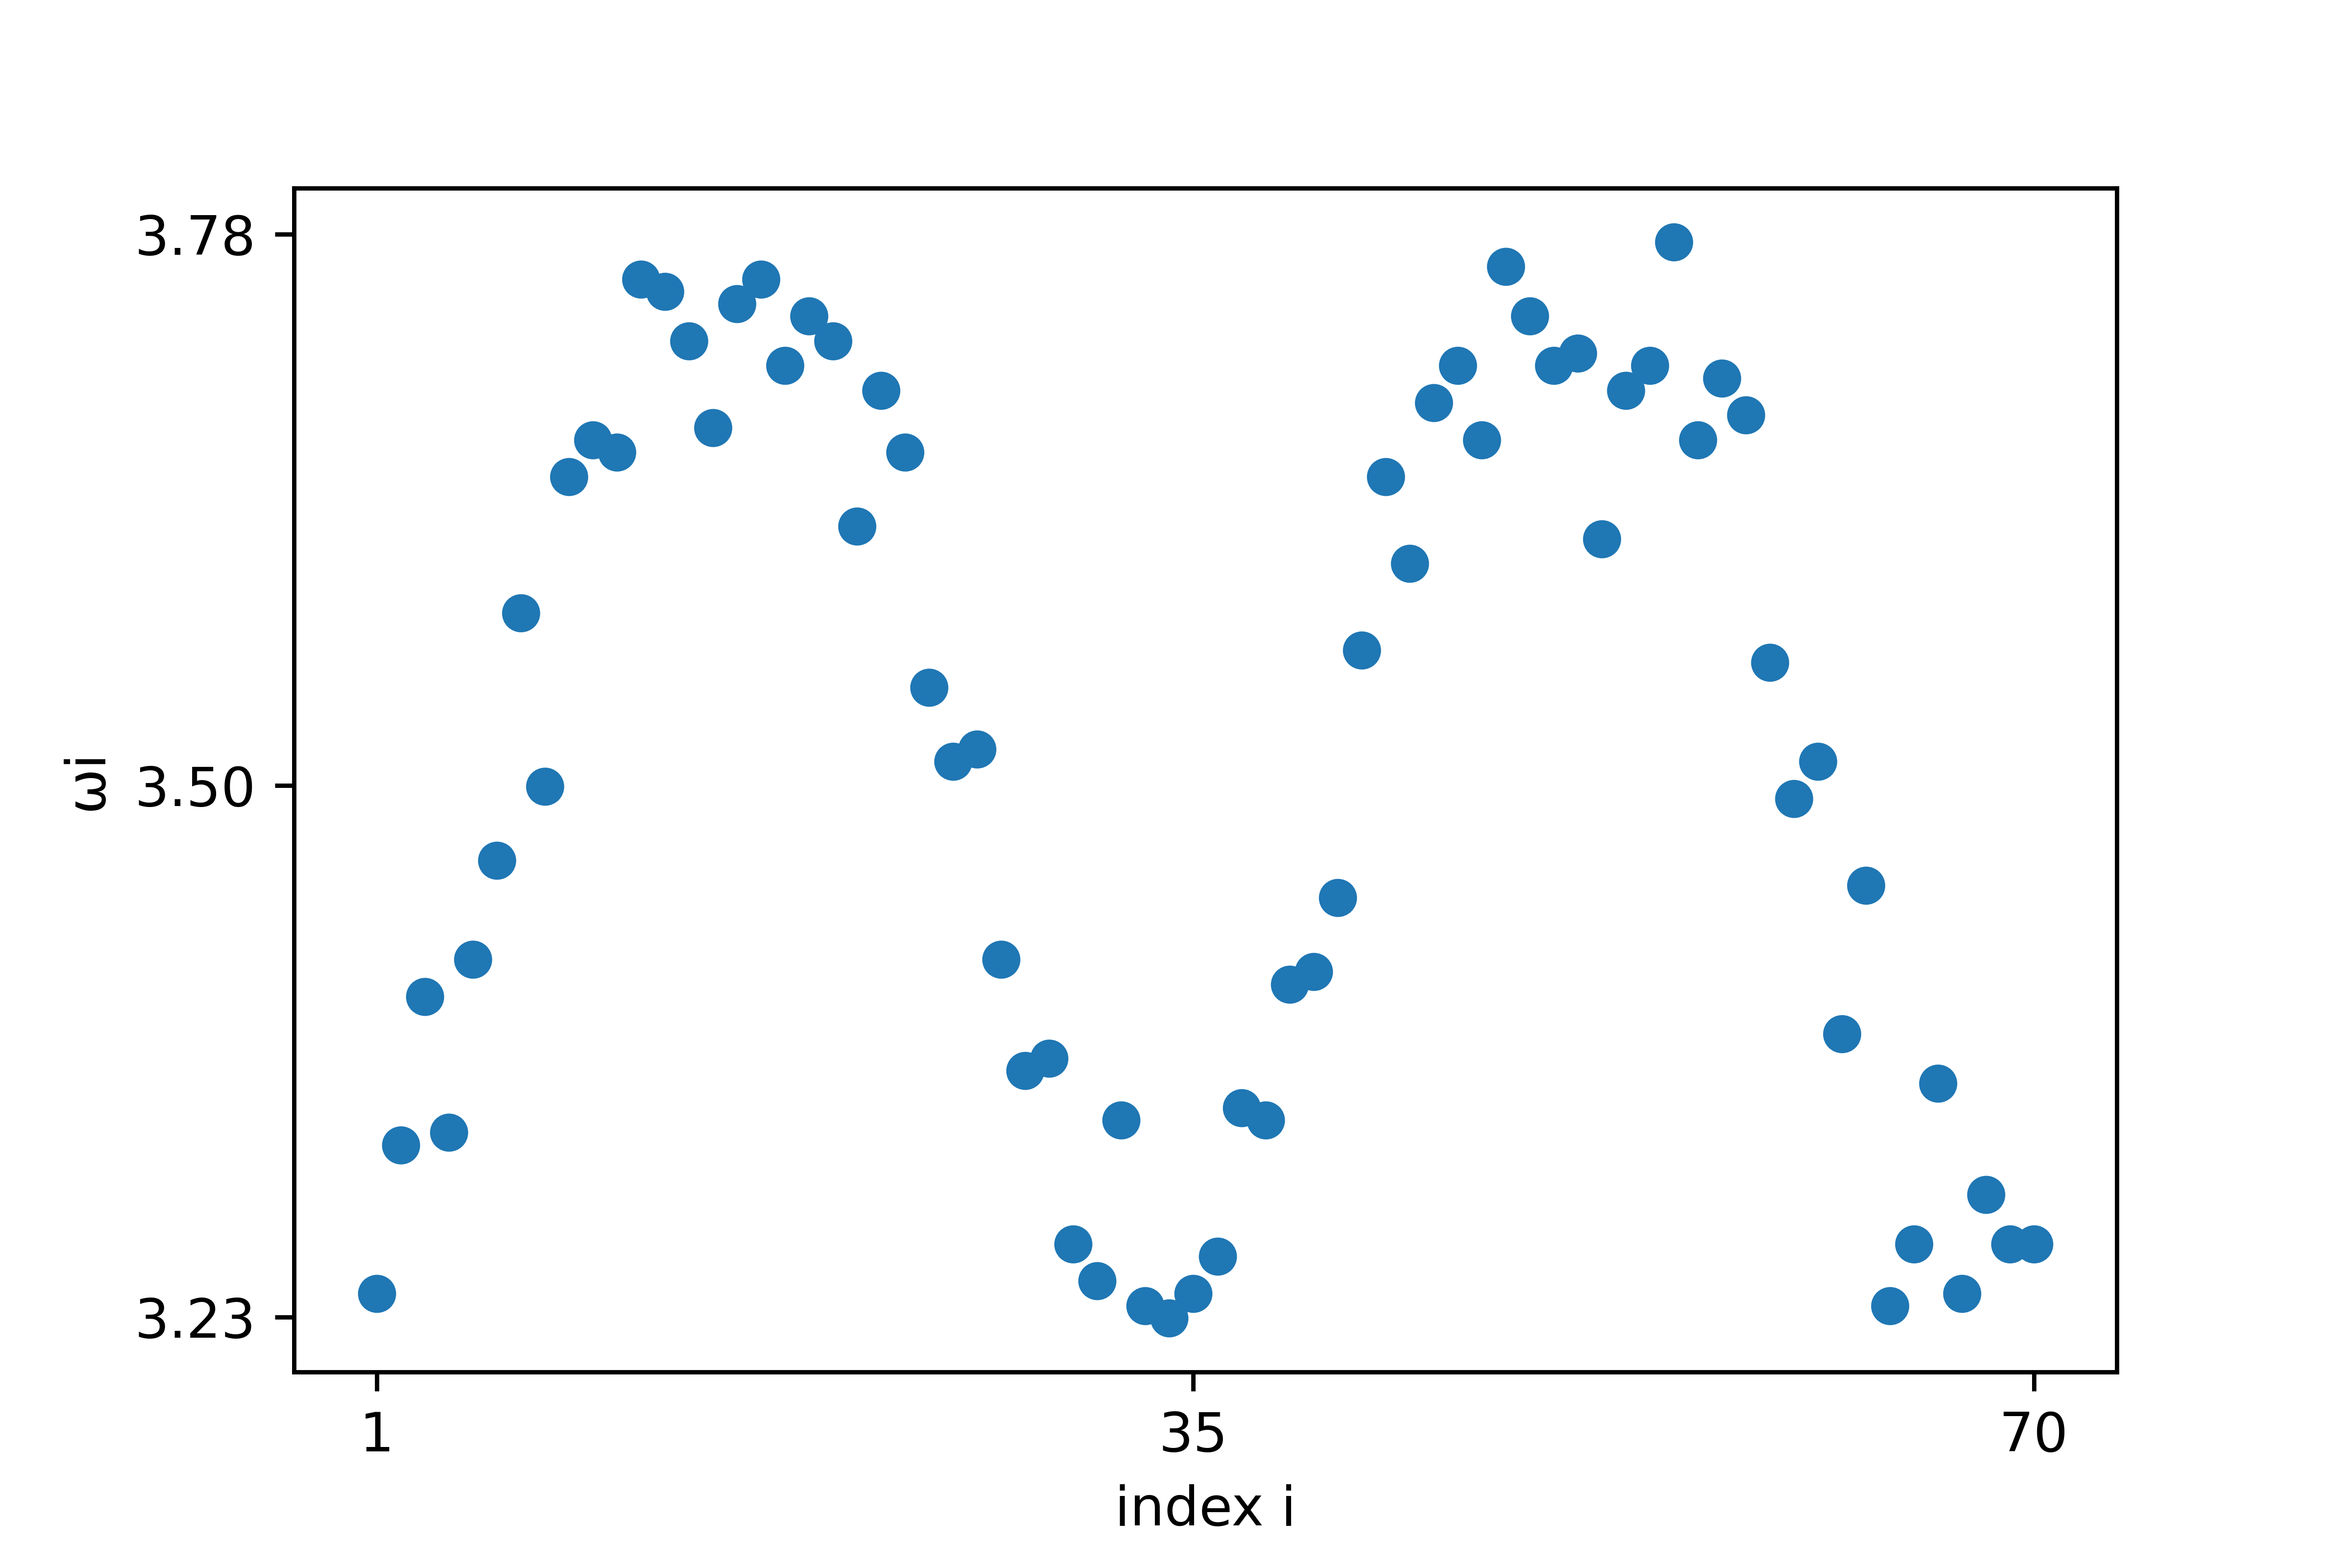
\includegraphics[width=1\linewidth]{w_sigma=1.7.png}  
  \caption{$\sigma = 1.7$}
\end{subfigure}
\caption{Snapshots of the membrane potential $u_i$ and mean phase-velocity profiles $\omega_i$ for the double chimeras observed, for $N=70$, $r=0.40$ at $t=1000$. The first row are the $u_i$ and the second row are the $\omega_i$.}
\label{dchim}
\end{figure}

\begin{figure}[H]
\centering
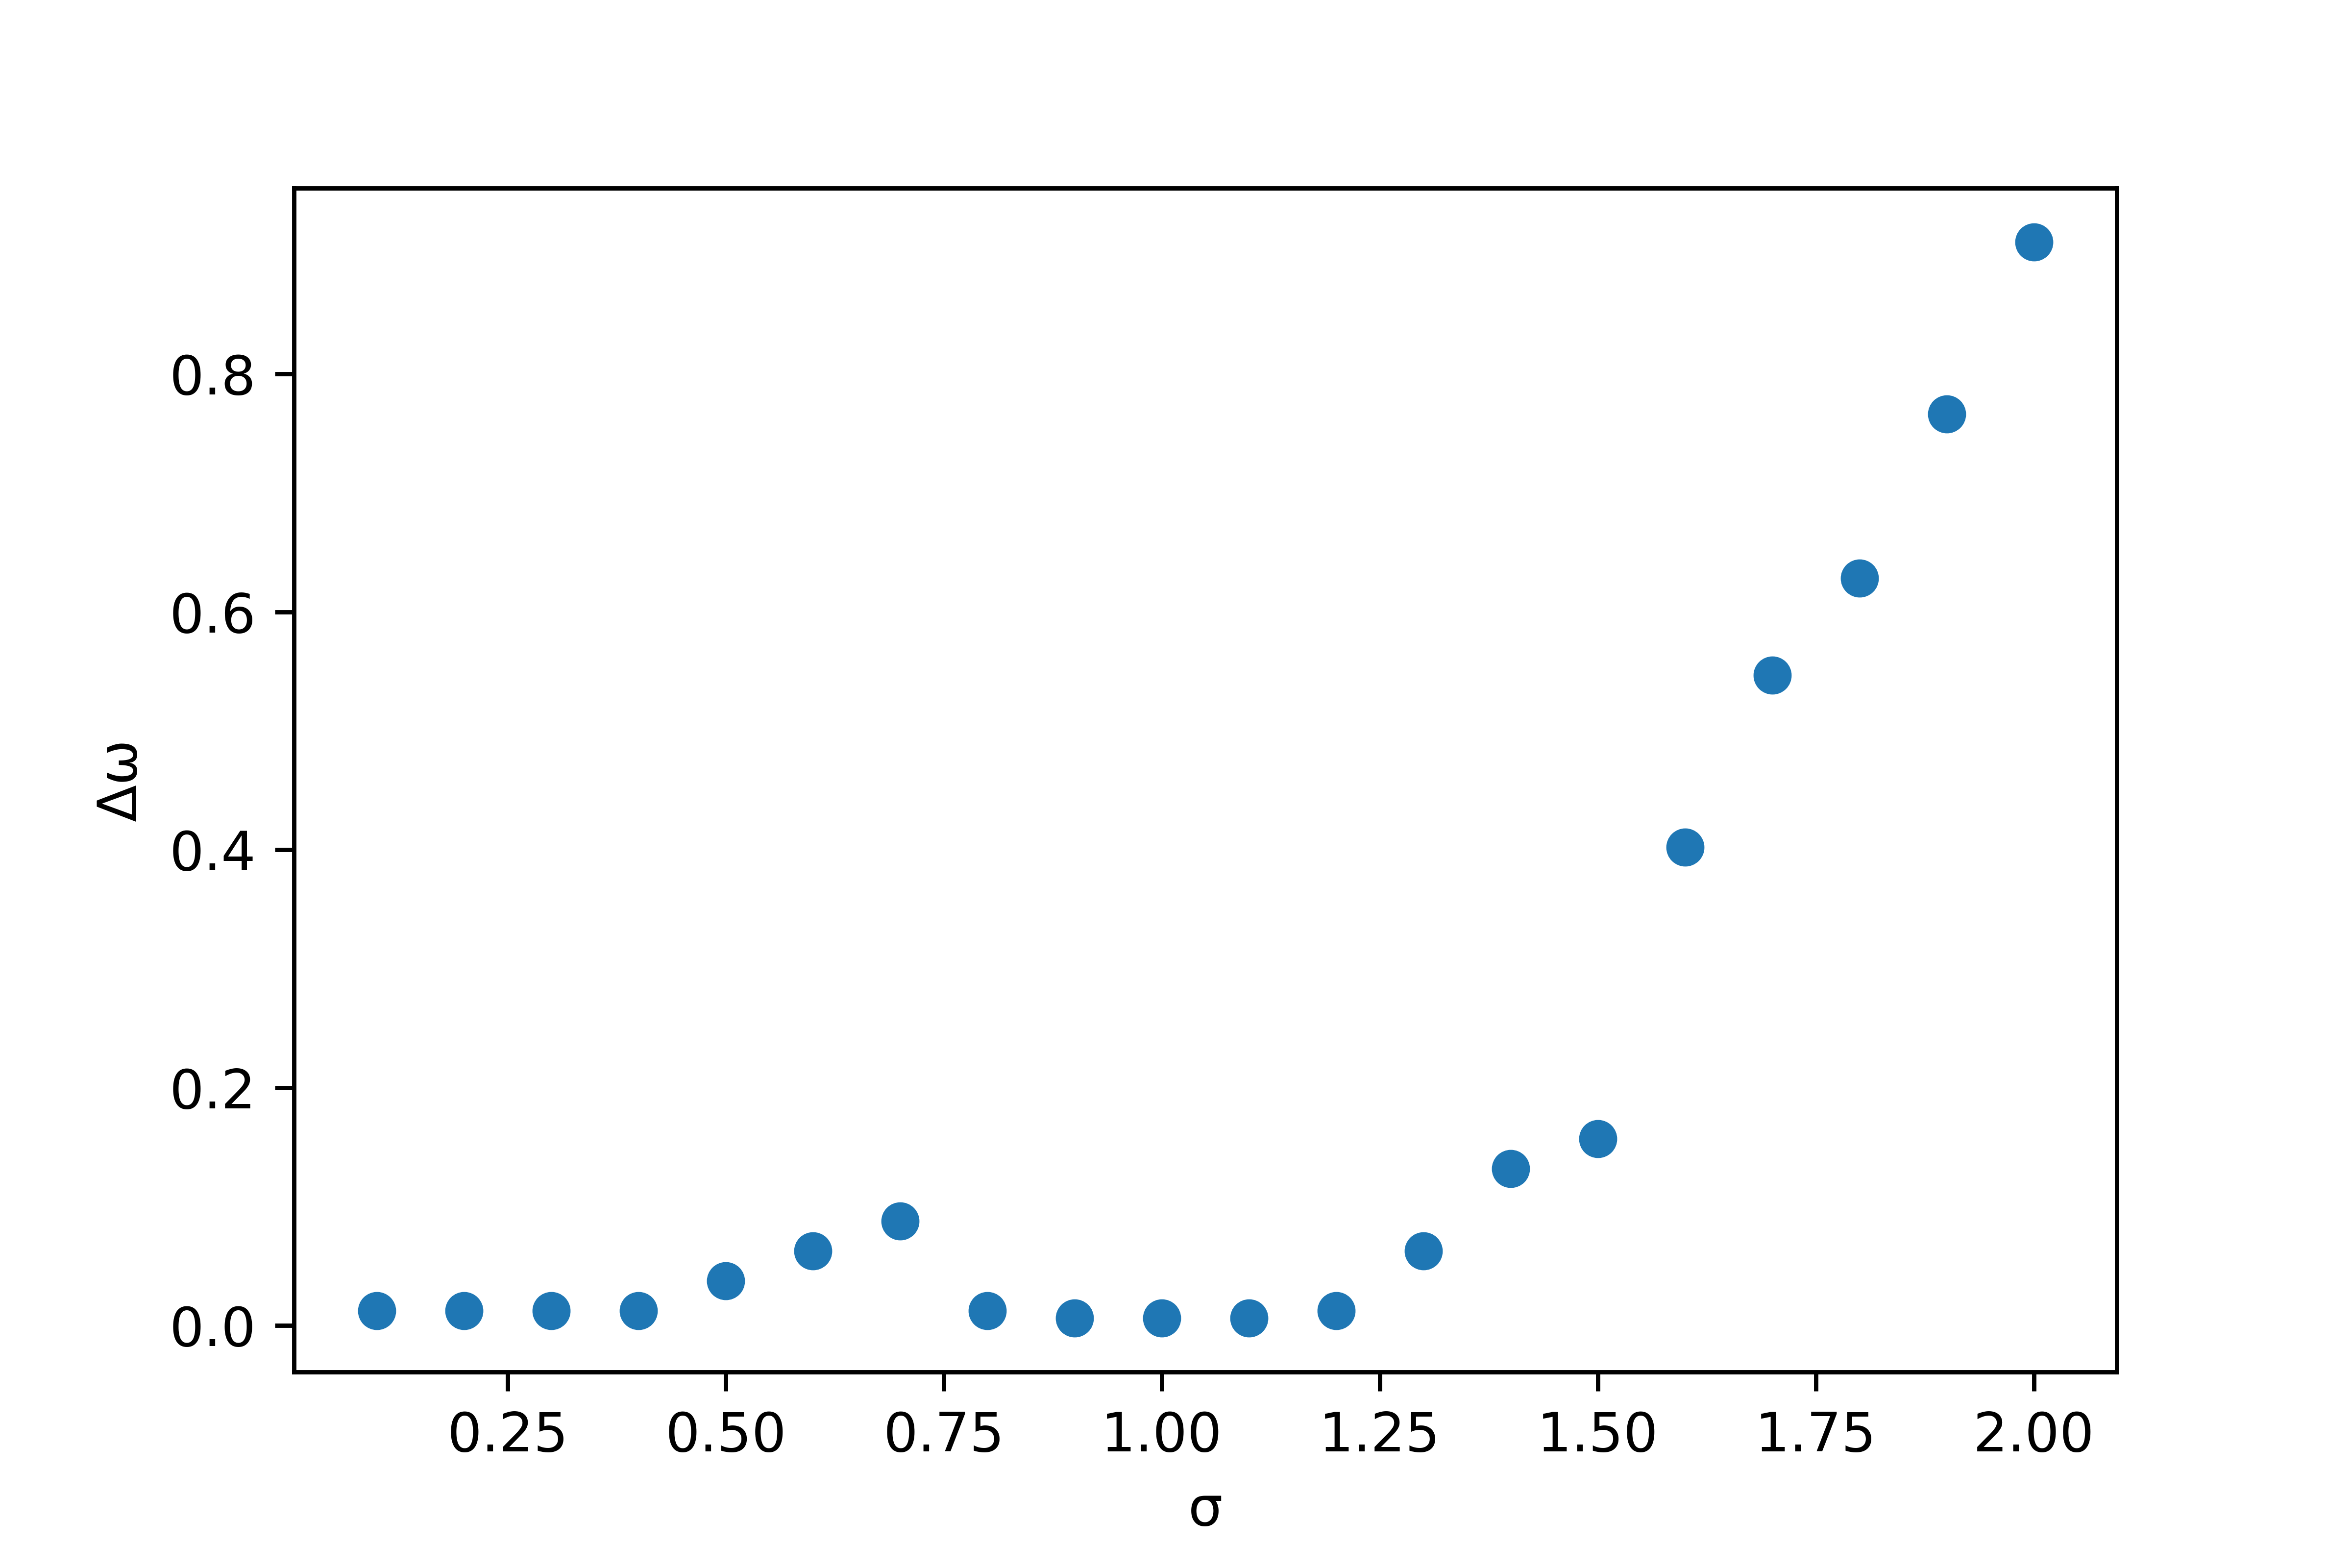
\includegraphics[width=0.6\textwidth]{deltaw.png}
\caption{$\Delta \omega = \omega_{\text{max}}-\omega_{\text{min}}$ with varying $\sigma$.}
\label{dchim2}
\end{figure}
\noindent The bump observed around $\sigma=0.7$ is due to the appearance of chimeras around this value of $\sigma$. After $\sigma = 1.4$ we see $\Delta \omega$ to increase, which also agrees with the observation of double chimeras for these values.

\subsection{Dependence on initial conditions}
We also investigate how the appearance of chimeras is dependent on the initial conditions. For $N=70$, $\sigma=0.7$ and $r=0.35$, we run the system for different seed numbers with the command \texttt{numpy.random.seed()}. We save snapshots at $t=1000$ and $t=4000$ time units. First, we notice that chimeras are highly dependent on the initial conditions because there are seed numbers which result in chimeras (Fig. (\ref{chim})) while others that results in ``chain-like'' synchronisation (Fig. (\ref{chain})).
\begin{figure}[H]
\begin{subfigure}{0.49 \textwidth}
\centering
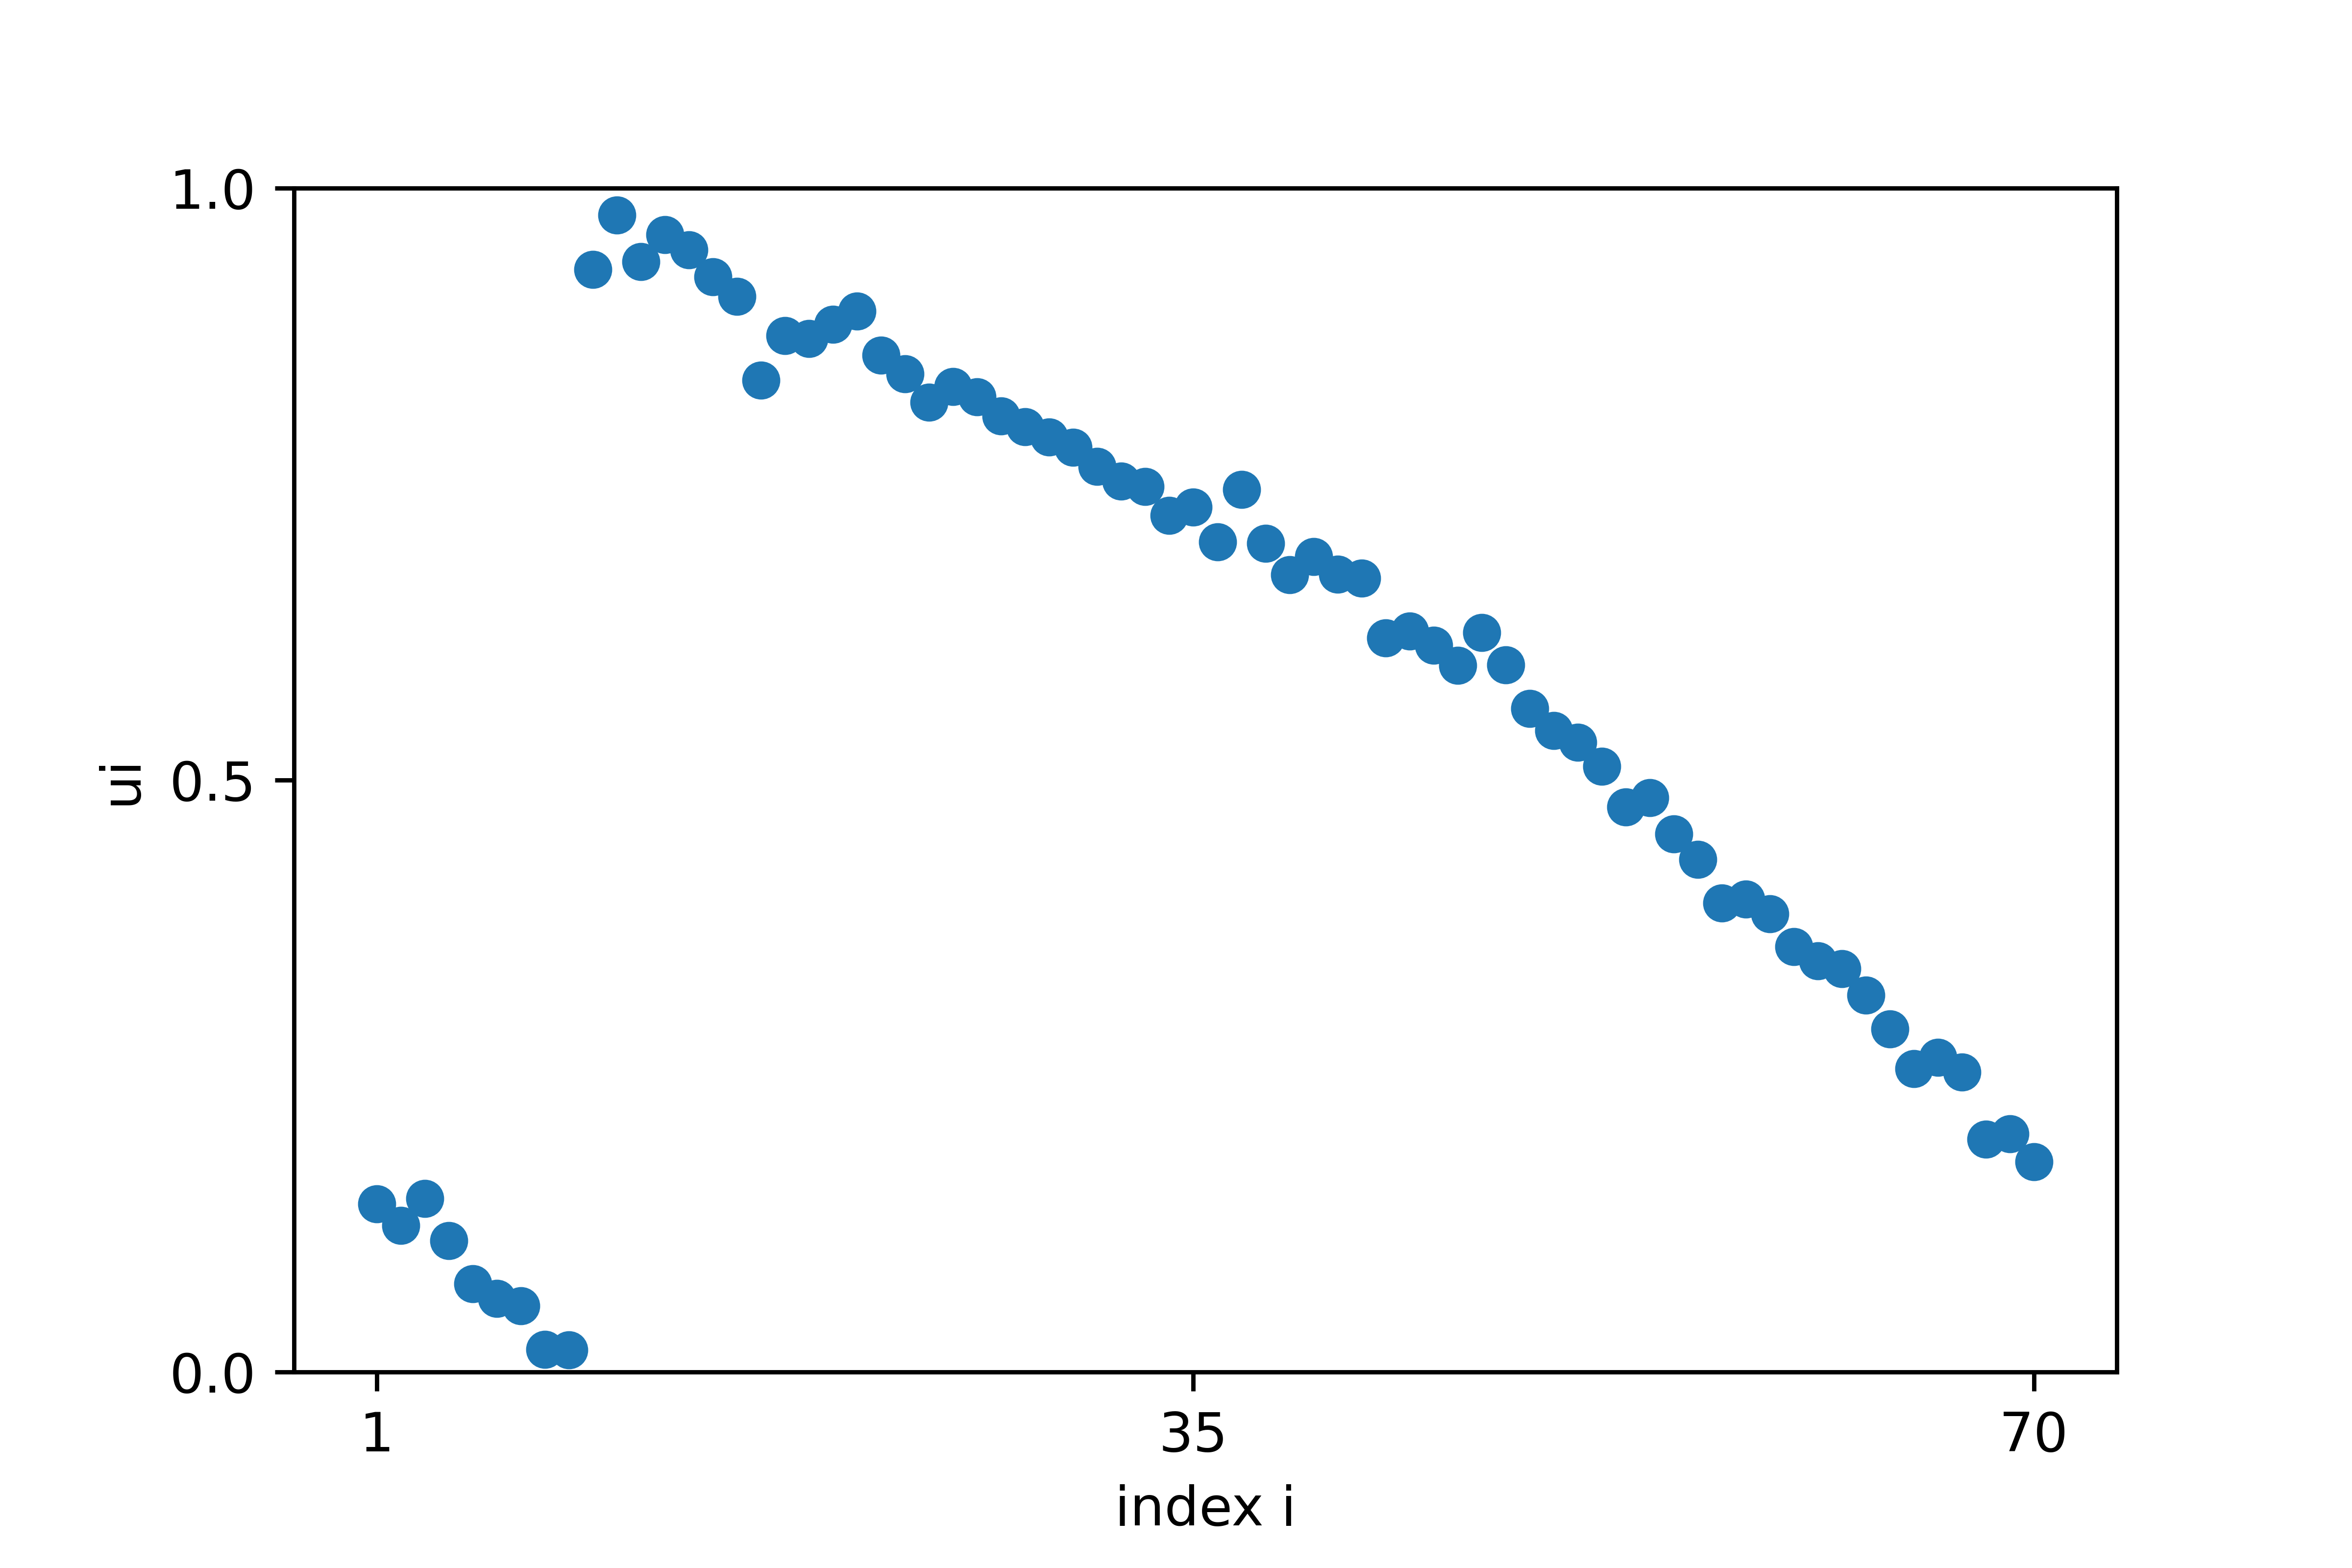
\includegraphics[width=\linewidth]{u_seed=64856_t=1000.png}
\caption{seed = $64856$}
\label{chain}
\end{subfigure}
\hfill
\begin{subfigure}{0.49 \textwidth}
\centering
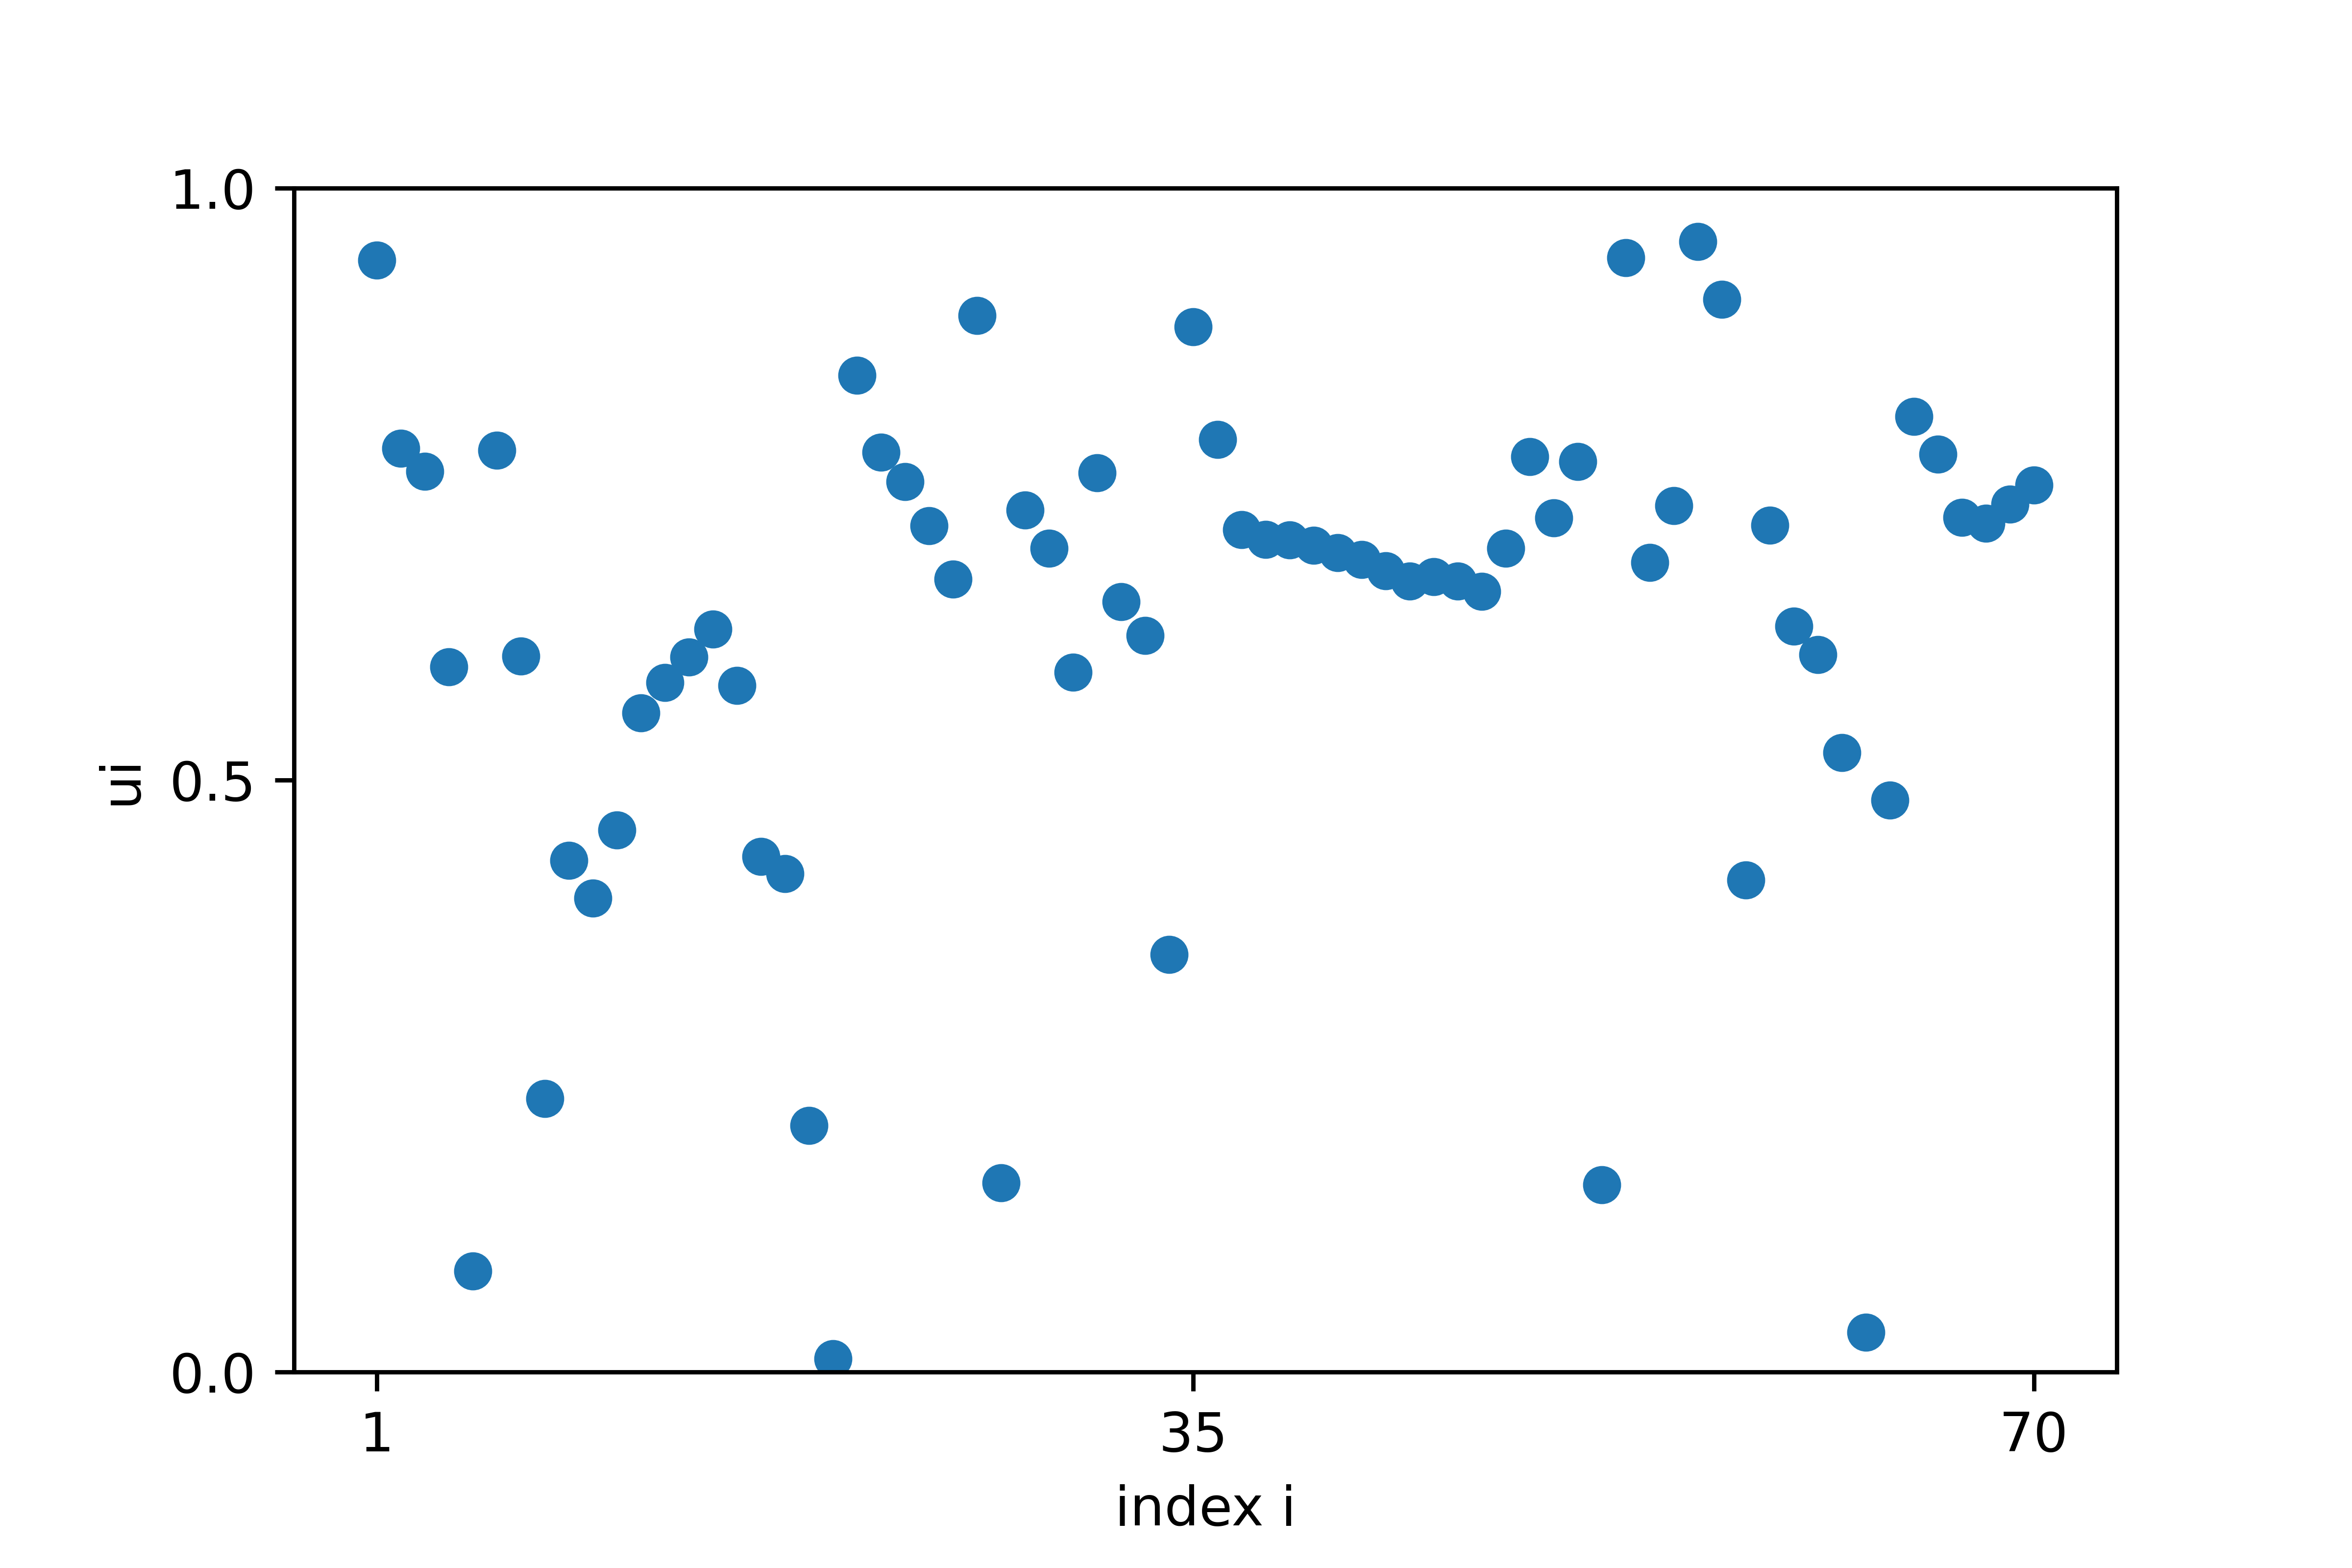
\includegraphics[width=\linewidth]{u_seed=38958_t=1000.png}
\caption{seed = $38958$} 
\label{chim}
\end{subfigure}
\caption{Snapshots of the membrane potential $u_i$ at $t=1000$, for $N=70$, $\sigma=0.7$ and $r=0.35$, for two different initial conditions.}
\end{figure} 
\noindent On the other hand, we have cases where chimeras are transient (Fig. (\ref{trans})) and others that are not (Fig. (\ref{notrans})). 

\begin{figure}[H]
\begin{subfigure}{0.49 \textwidth}
\centering
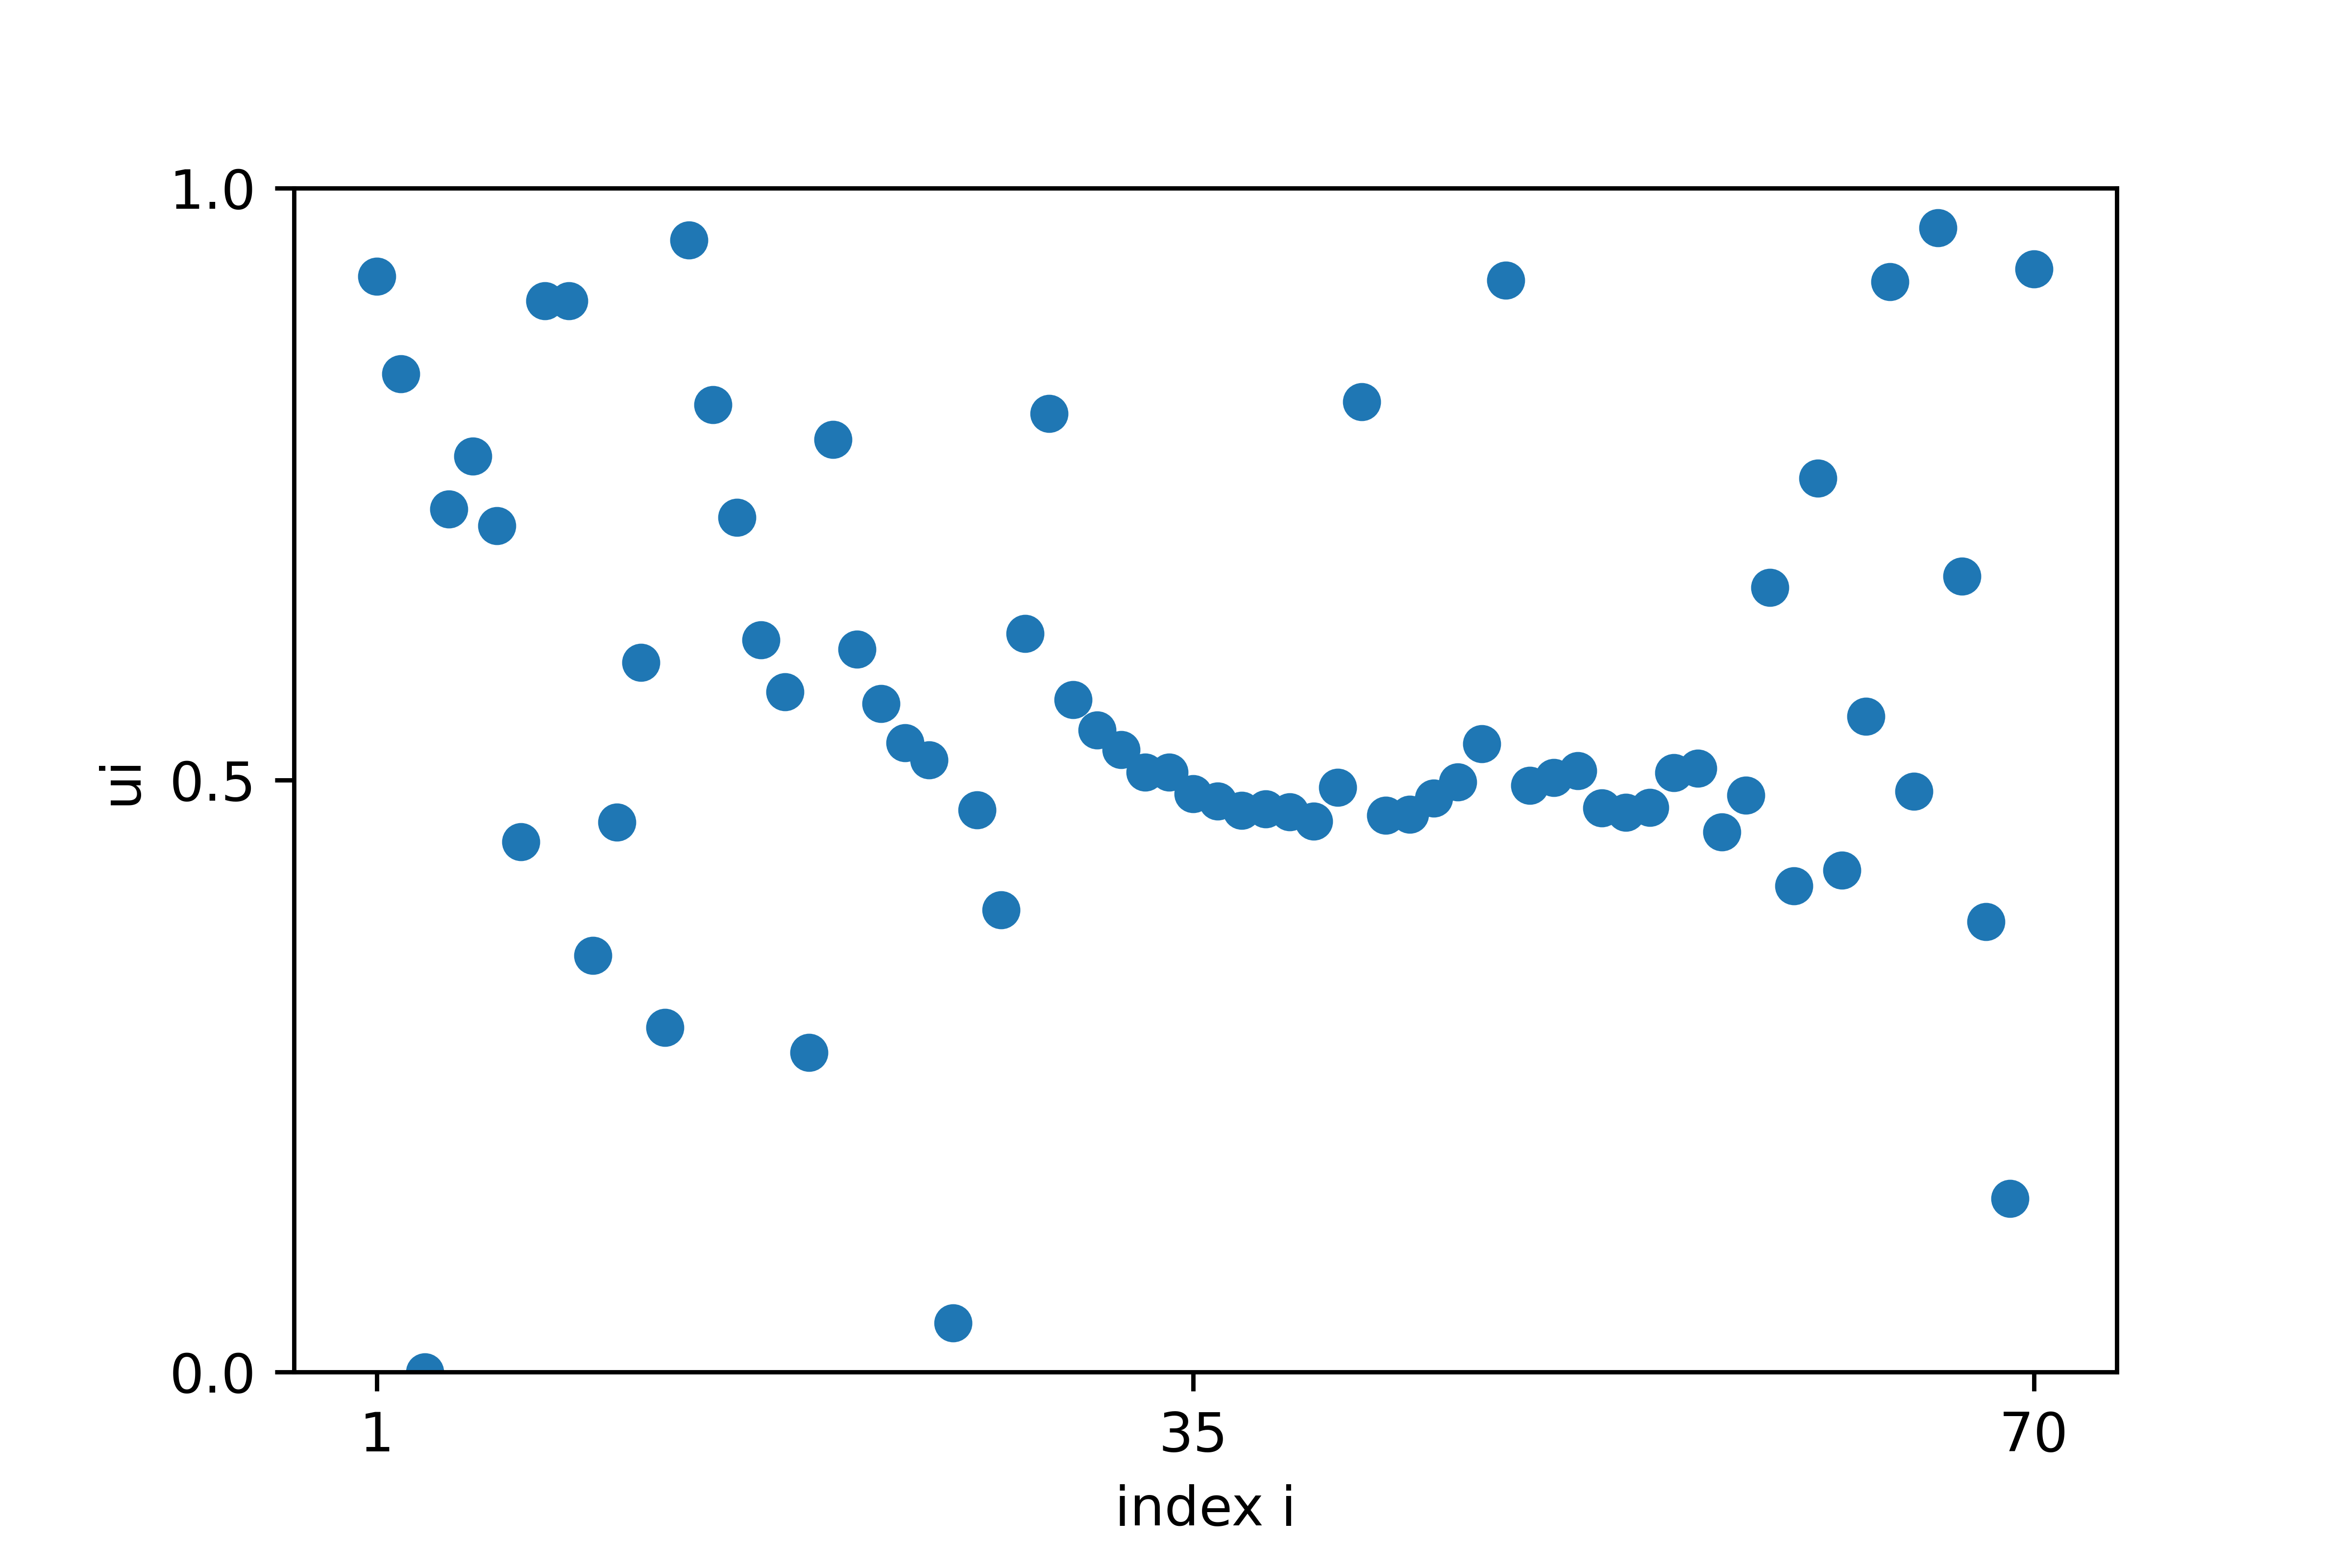
\includegraphics[width=\linewidth]{u_seed=70893_t=1000.png}
\caption{$t=1000$, seed = $70893$}

\end{subfigure}
\hfill
\begin{subfigure}{0.49 \textwidth}
\centering
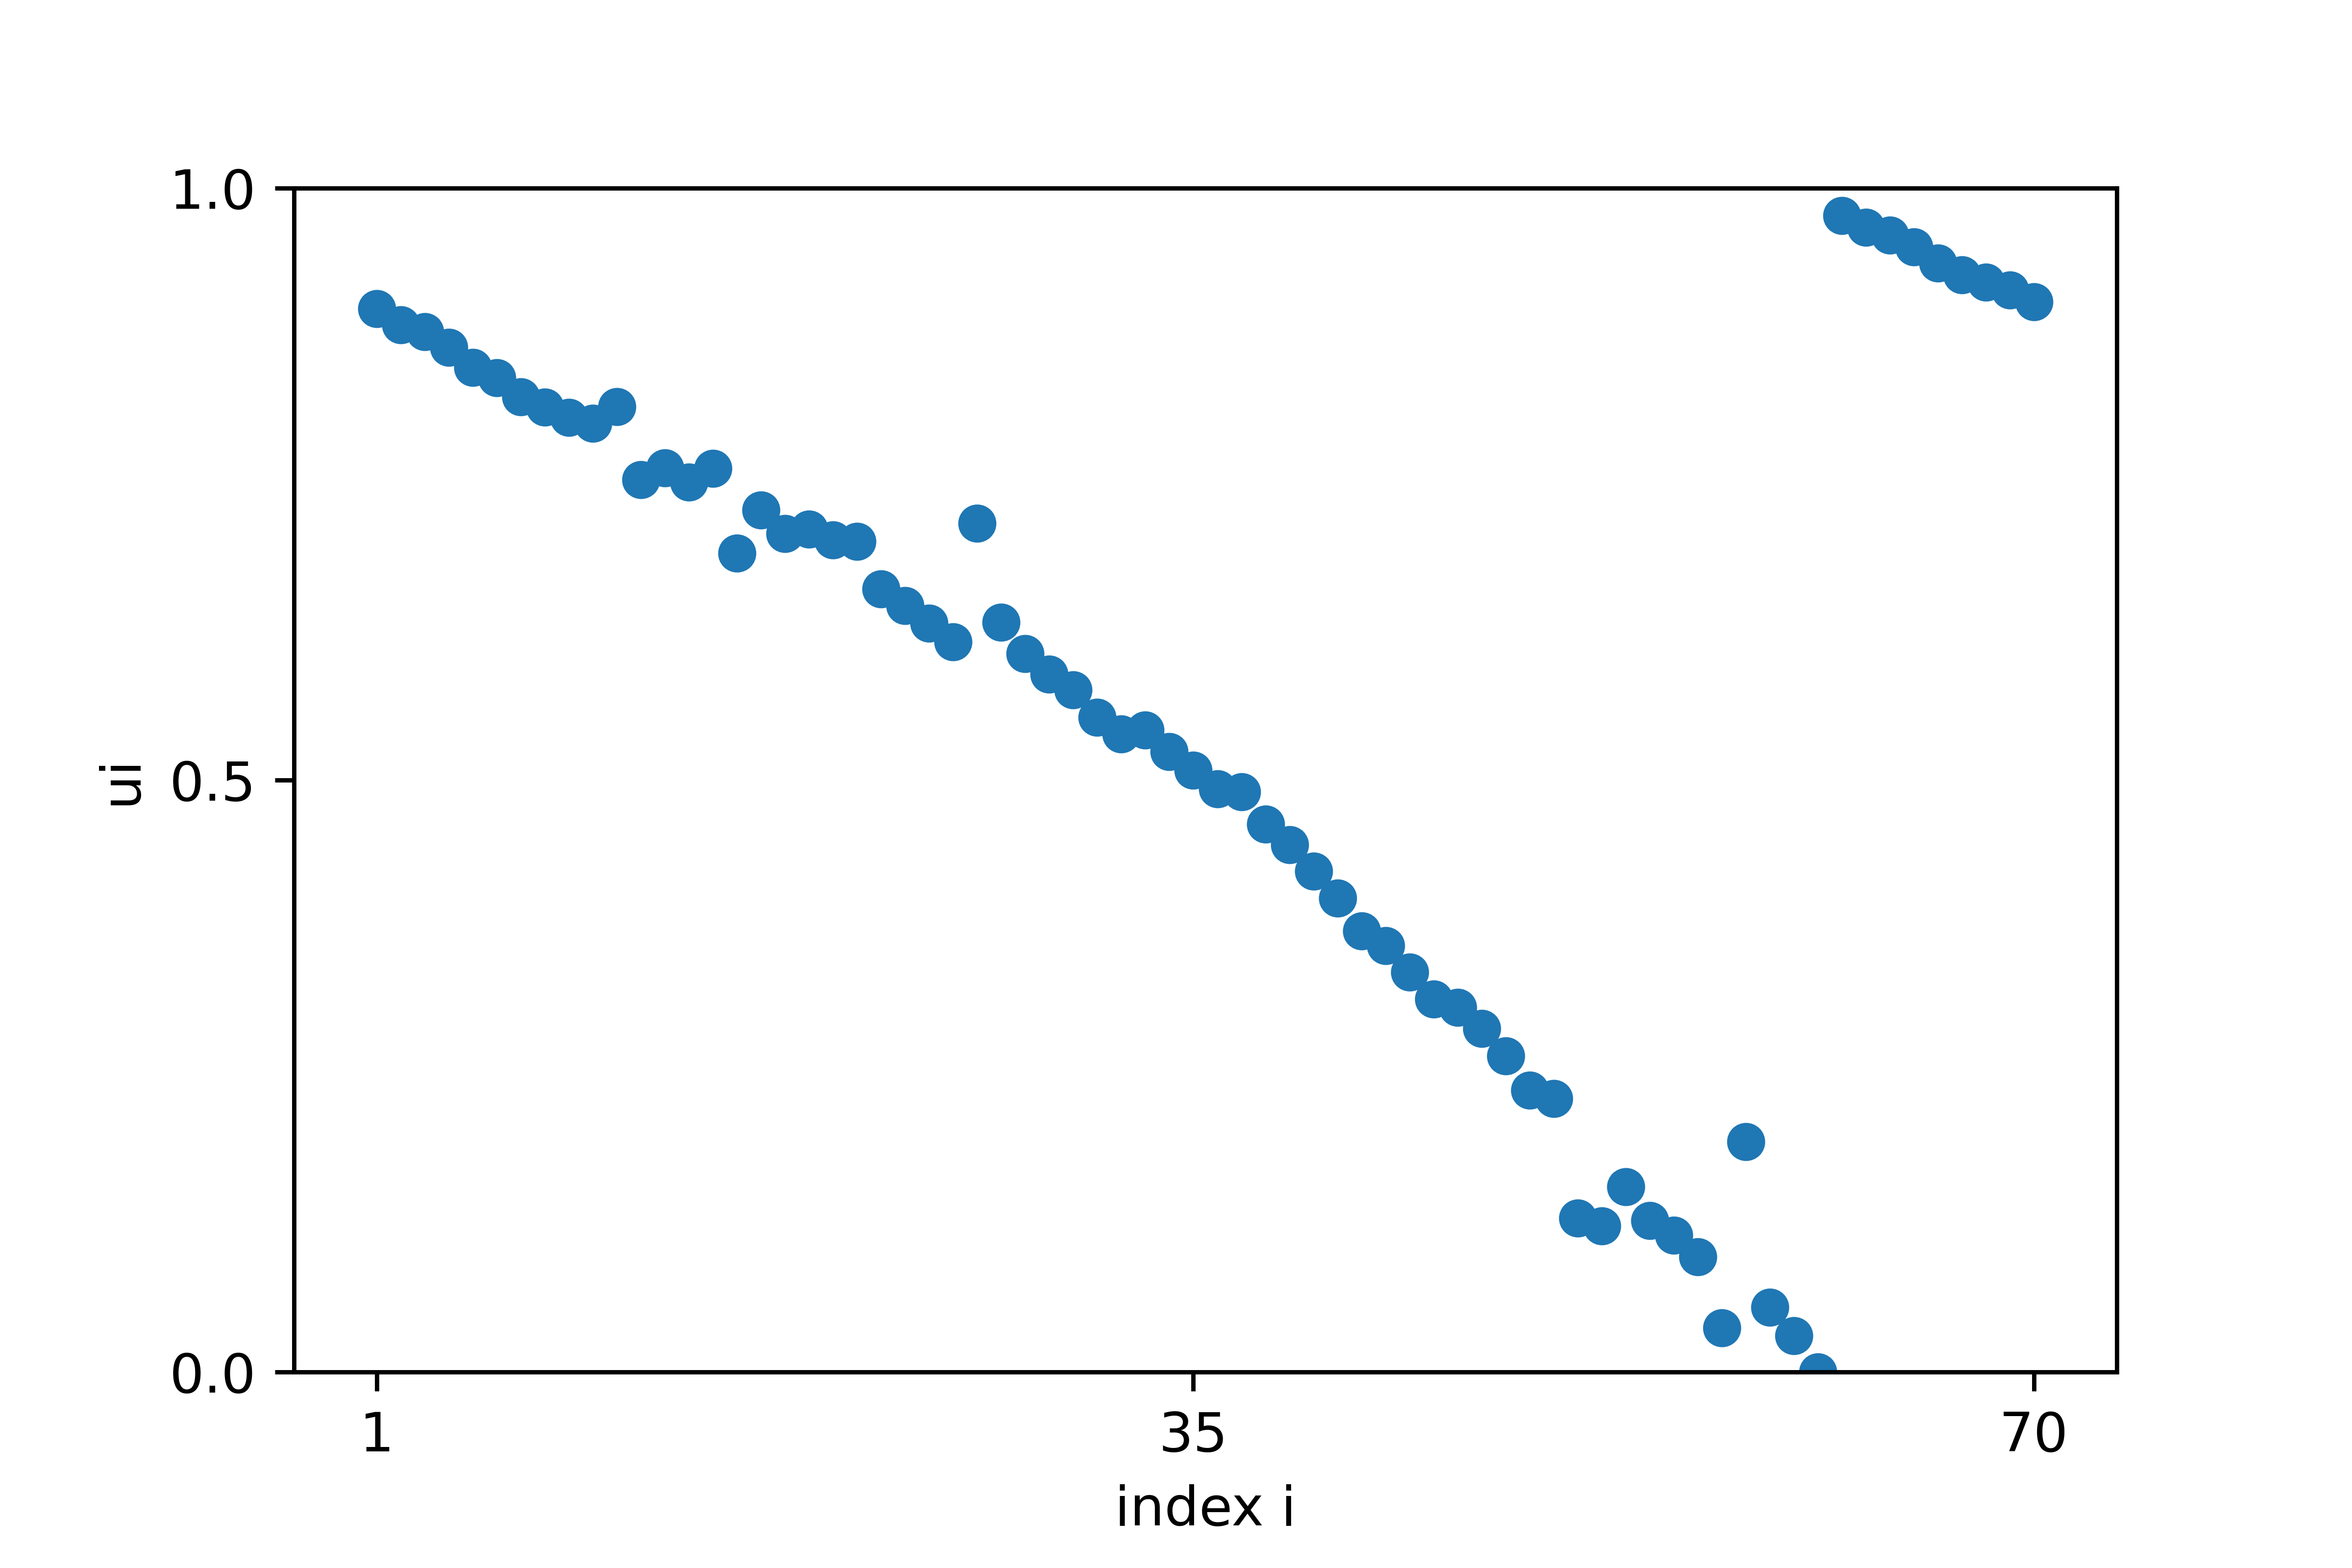
\includegraphics[width=\linewidth]{u_seed=70893_t=4000.png}
\caption{$t=4000$, seed = $70893$} 

\end{subfigure}
\caption{Snapshots of the membrane potential $u_i$, for $N=70$, $\sigma=0.7$ and $r=0.35$, at $t=1000$ and $t=4000$.}
\label{trans}
\end{figure} 

\begin{figure}[H]
\begin{subfigure}{0.49 \textwidth}
\centering
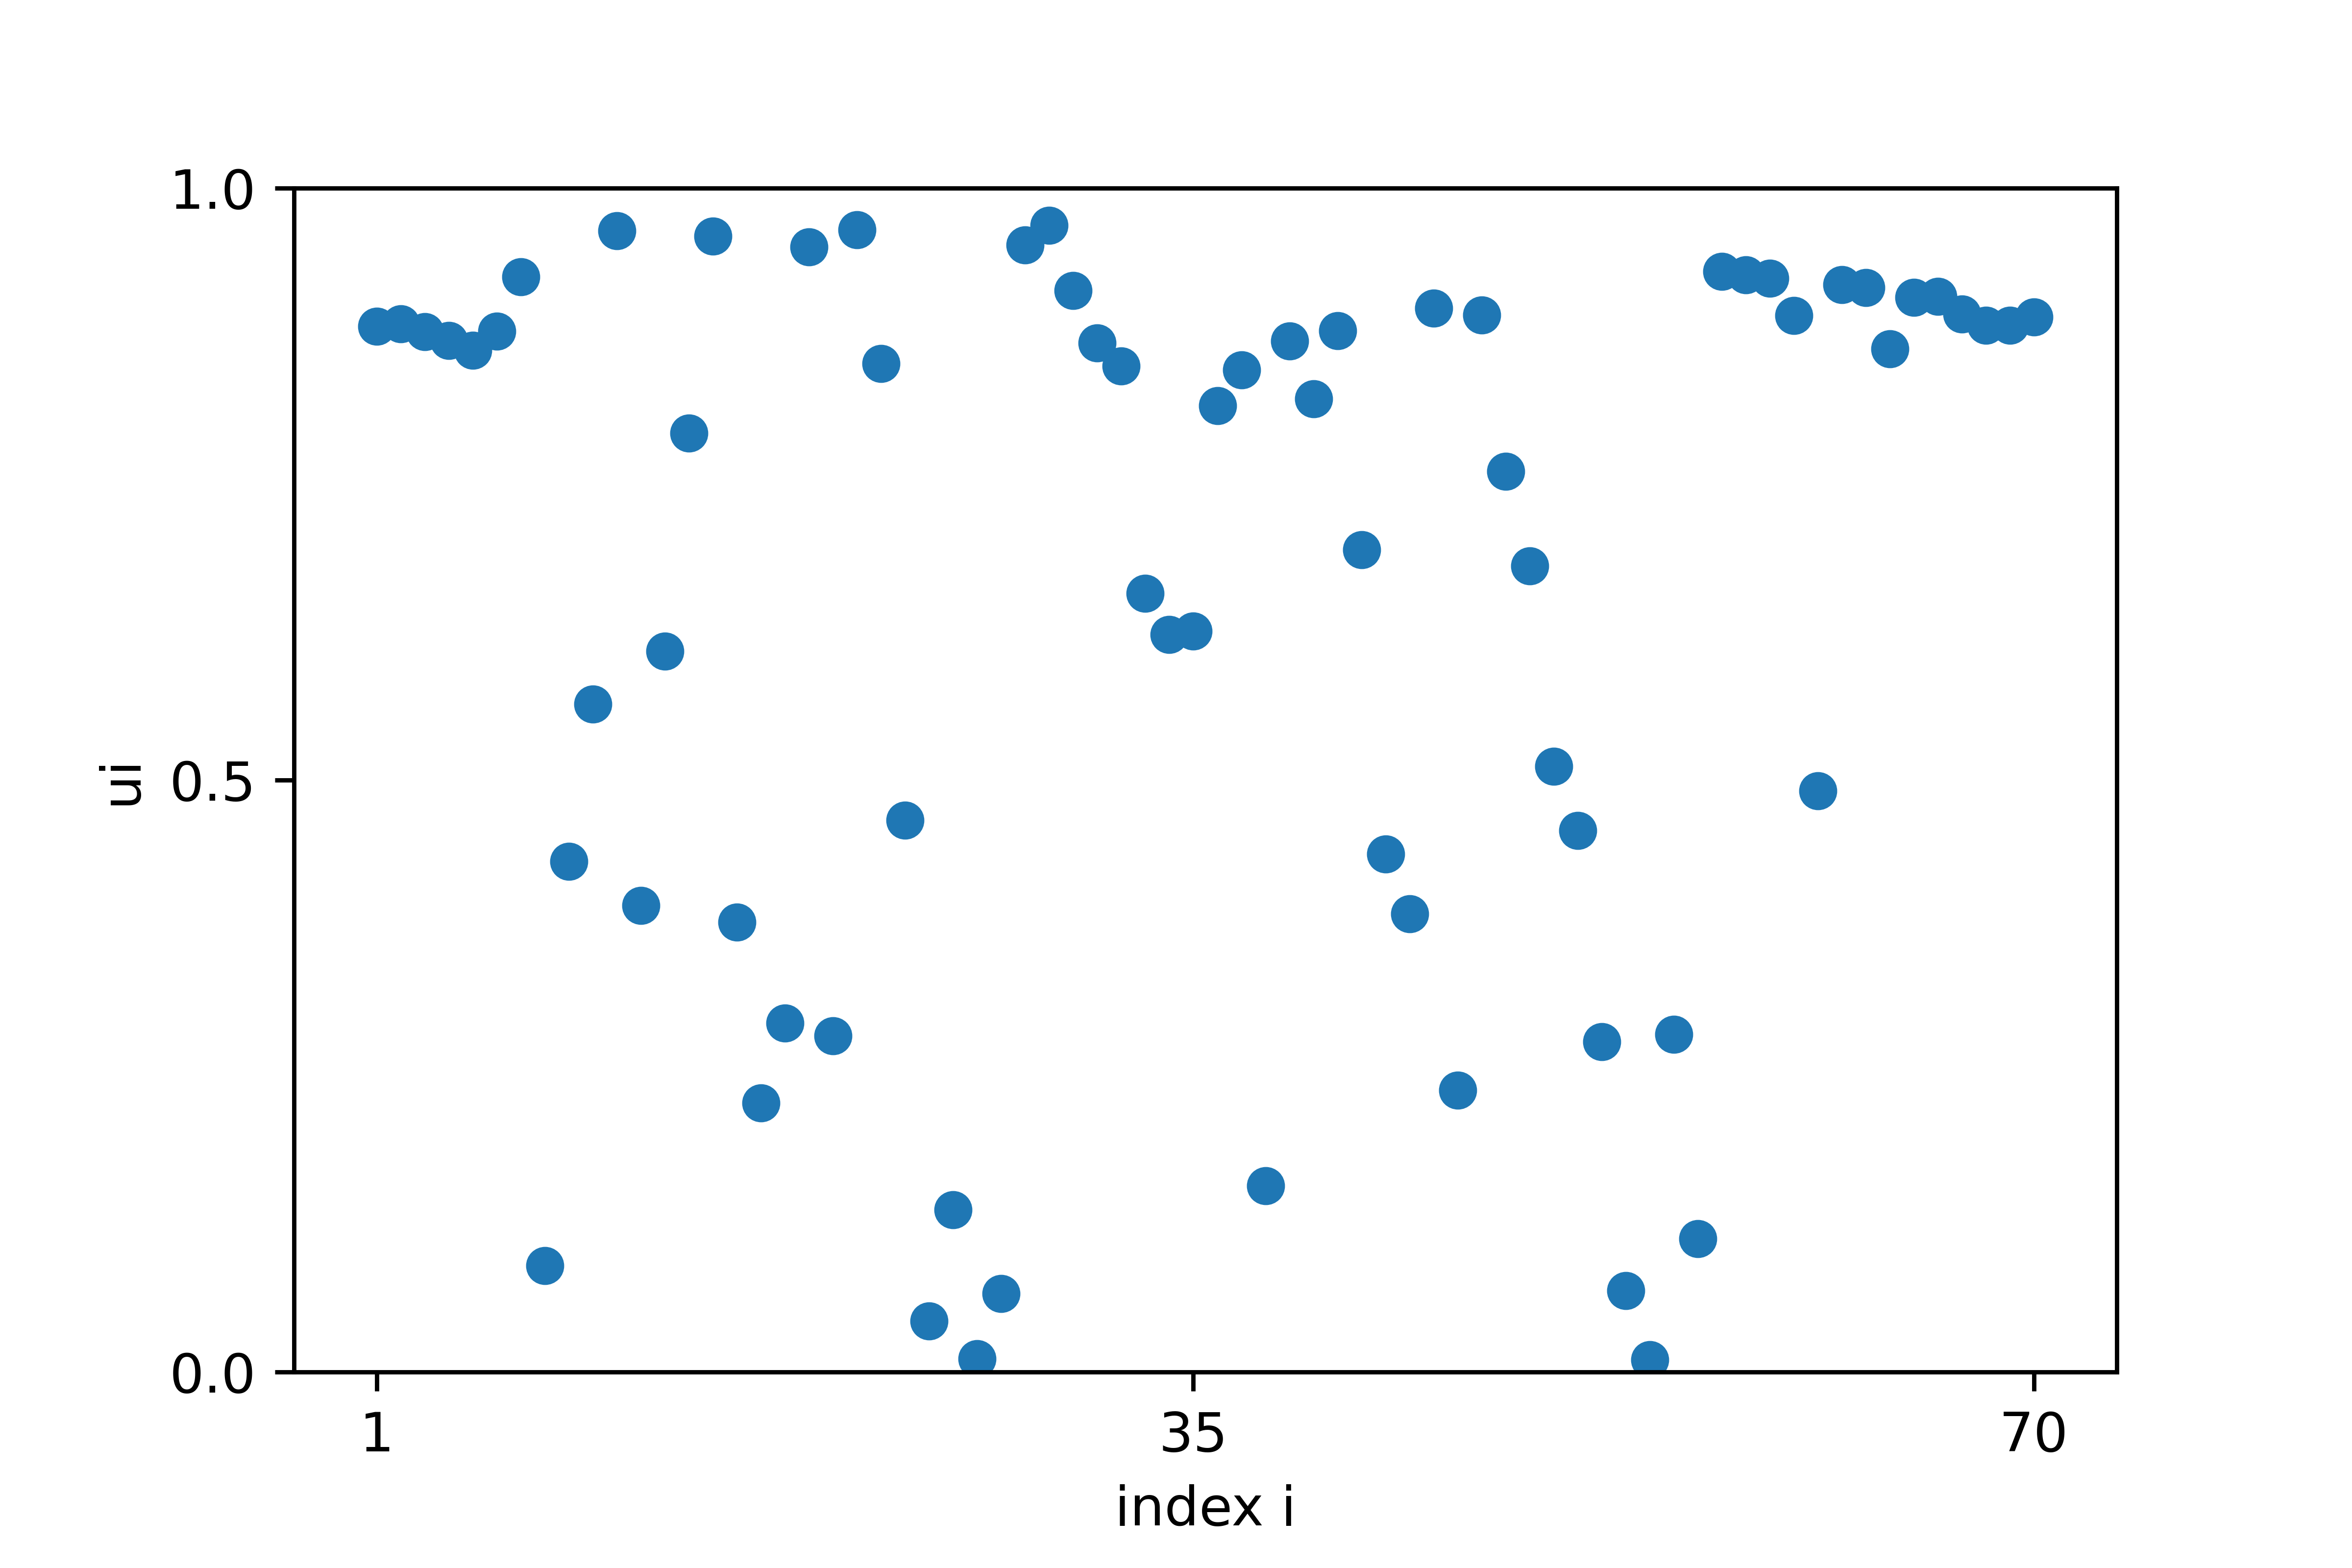
\includegraphics[width=\linewidth]{u_seed=27027_t=1000.png}
\caption{$t=1000$, seed = $27027$}
\end{subfigure}
\hfill
\begin{subfigure}{0.49 \textwidth}
\centering
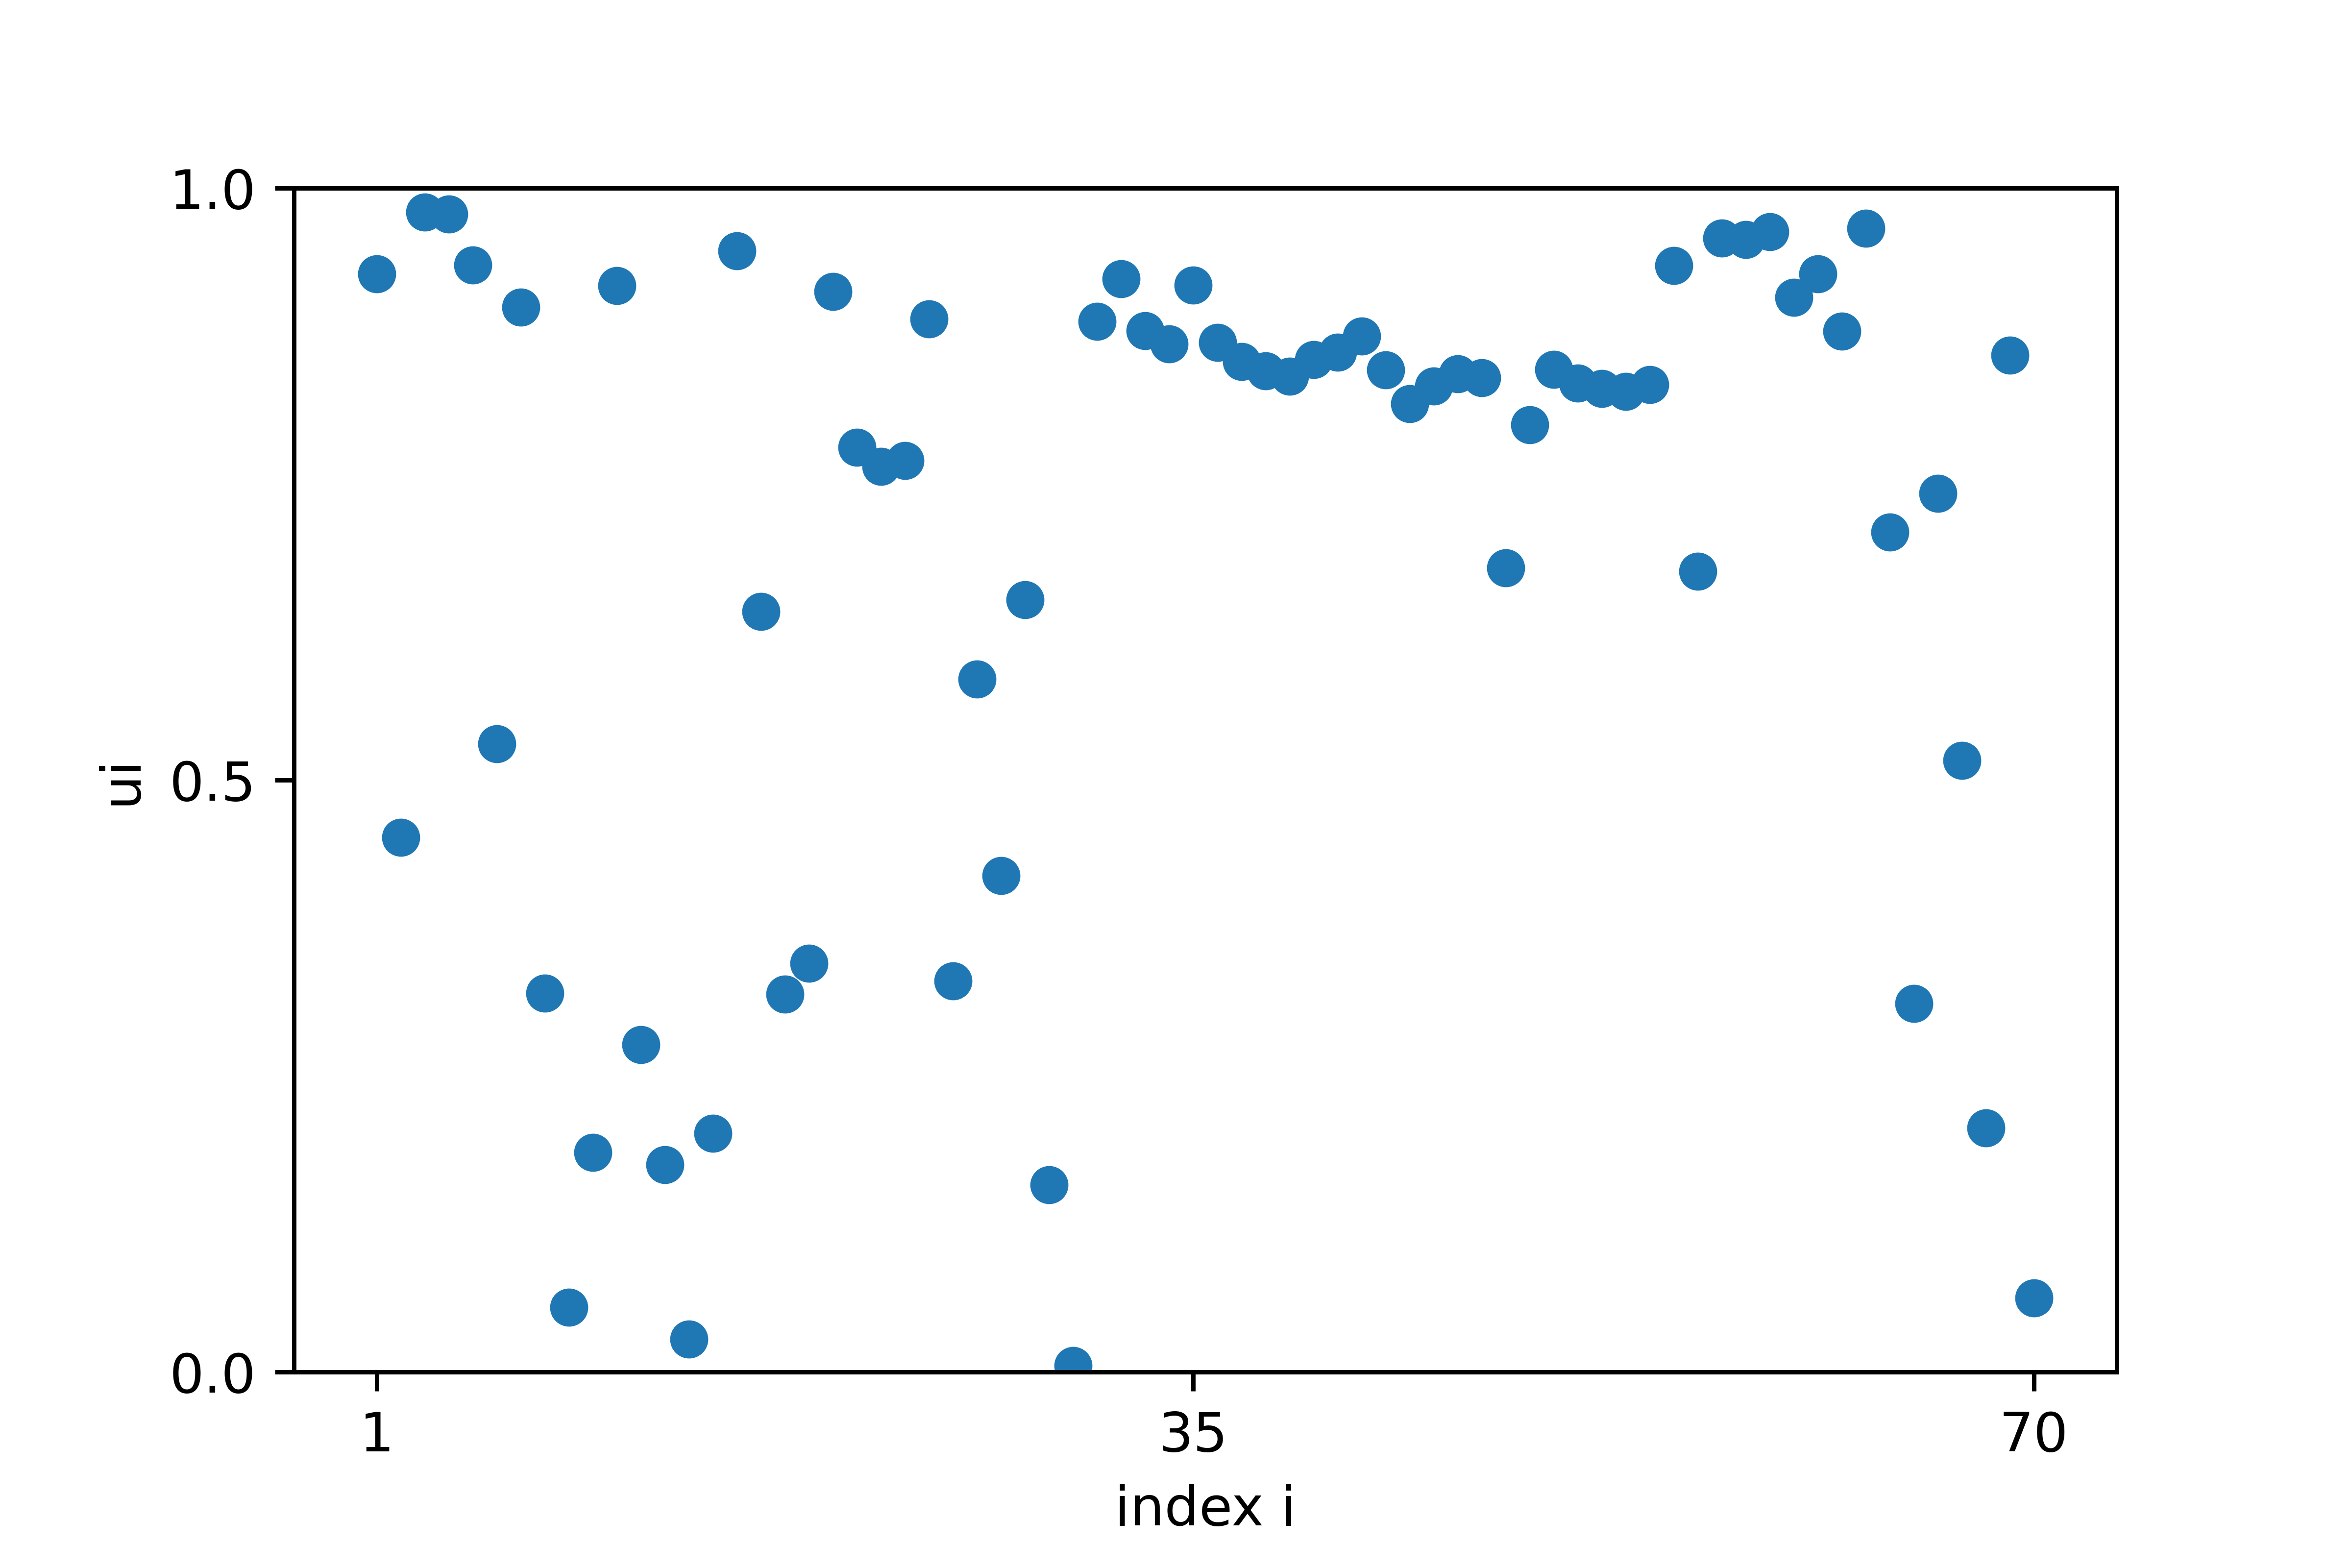
\includegraphics[width=\linewidth]{u_seed=27027_t=4000.png}
\caption{$t=4000$, seed = $27027$} 
\end{subfigure}
\caption{Snapshots of the membrane potential $u_i$ at $t=1000$ and $t=4000$, for $N=70$, $\sigma=0.7$ and $r=0.35$.}
\label{notrans}
\end{figure} 
\noindent We note that the coherent (and incoherent) region of the chimera in Fig. (\ref{notrans}) is moving slowly with time. These chimeras are called ``travelling''.

\section{The modified LIF model}
We now study chimeras when we modify the LIF model by varying the parameter $\lambda$. 
\subsection{Chimeras states in the non-leaky integrate-and-fire model}
We start with setting $\lambda=0$. For $r=0.35$ we vary $\sigma$ from $0.1$ to $2.0$ in $0.1$ increments, running each model for $1000$ time units. We observe asynchronisation for $ 0.1 \leq \sigma \leq 0.8$ and $ 1.6 \leq \sigma \leq 2.0$. Therefore, we focus on the range $ 0.9 \leq \sigma \leq 1.5$. The most significant signature for a chimera is observed for $\sigma = 1.4$. For $N=200$, the snapshots for $t=1000$ and $t=4000$ time units are shown in Fig. (\ref{1.4}). The respective $\omega_i$ profile for $t=4000$ is also shown in Fig. (\ref{1.4omega}).

\begin{figure}[H]
\begin{subfigure}{0.49 \textwidth}
\centering
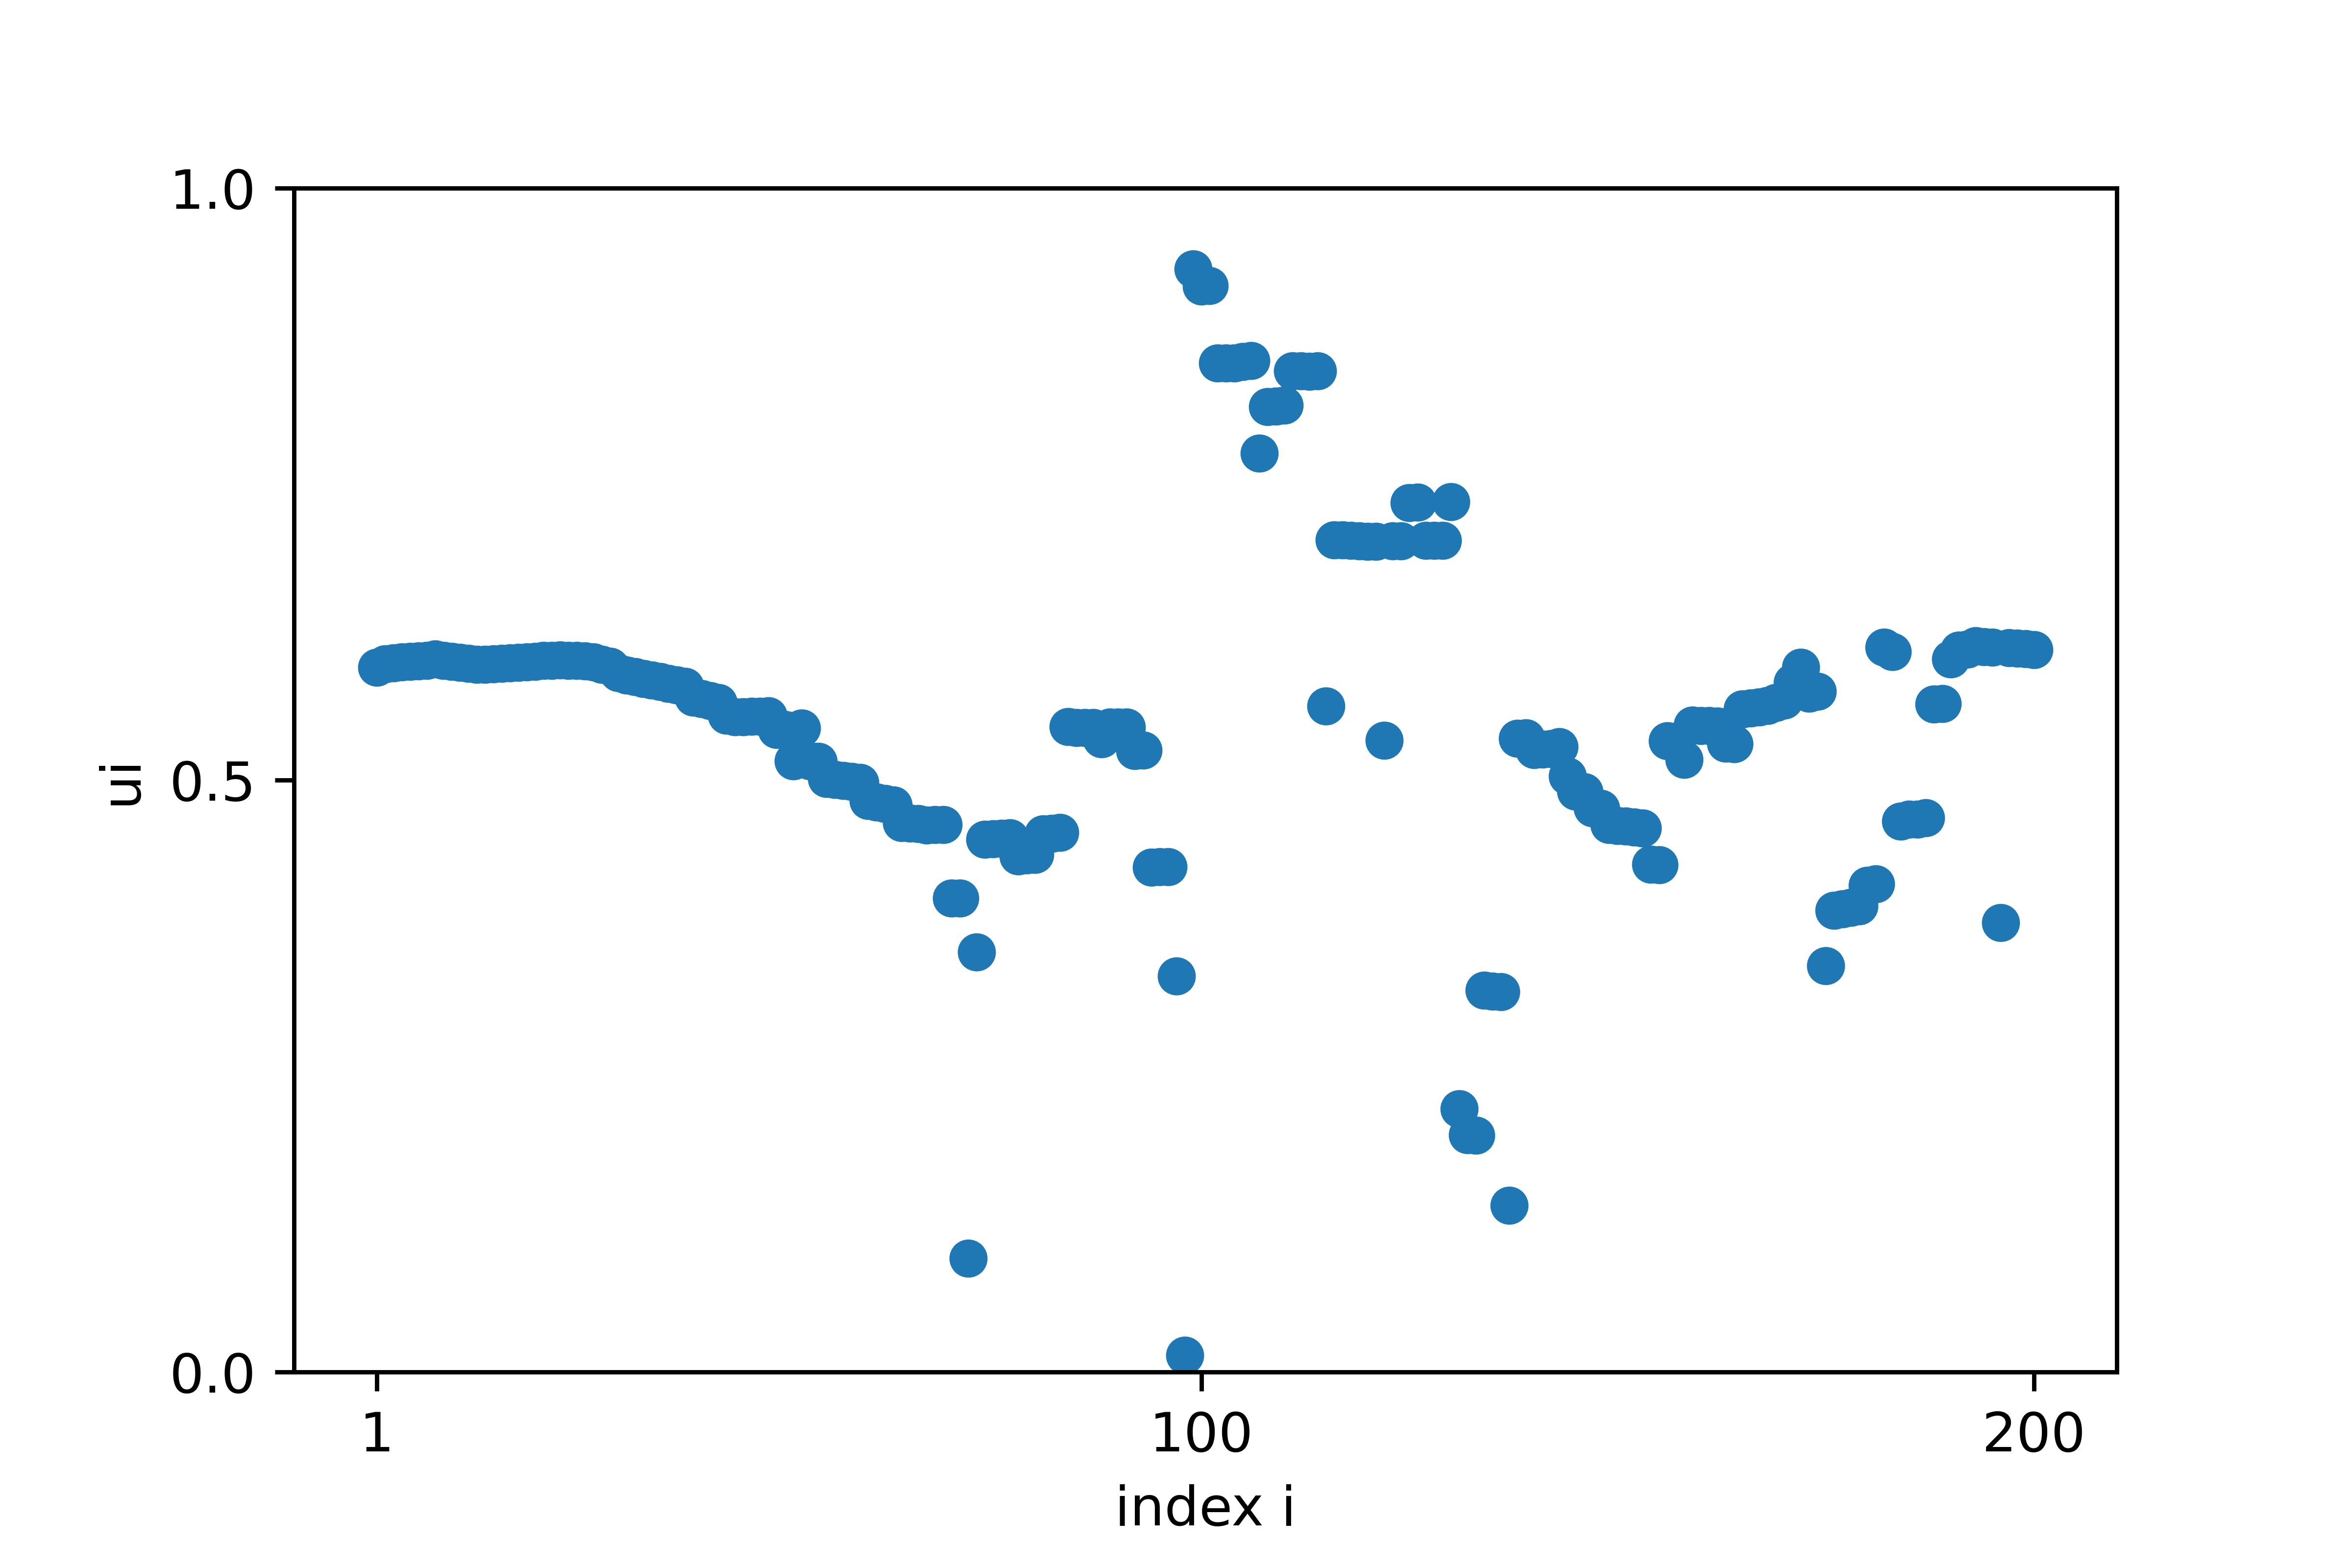
\includegraphics[width=\linewidth]{u_N=200_sigma=1.4_t=1000.png}
\caption{$t=1000$}
\end{subfigure}
\hfill
\begin{subfigure}{0.49 \textwidth}
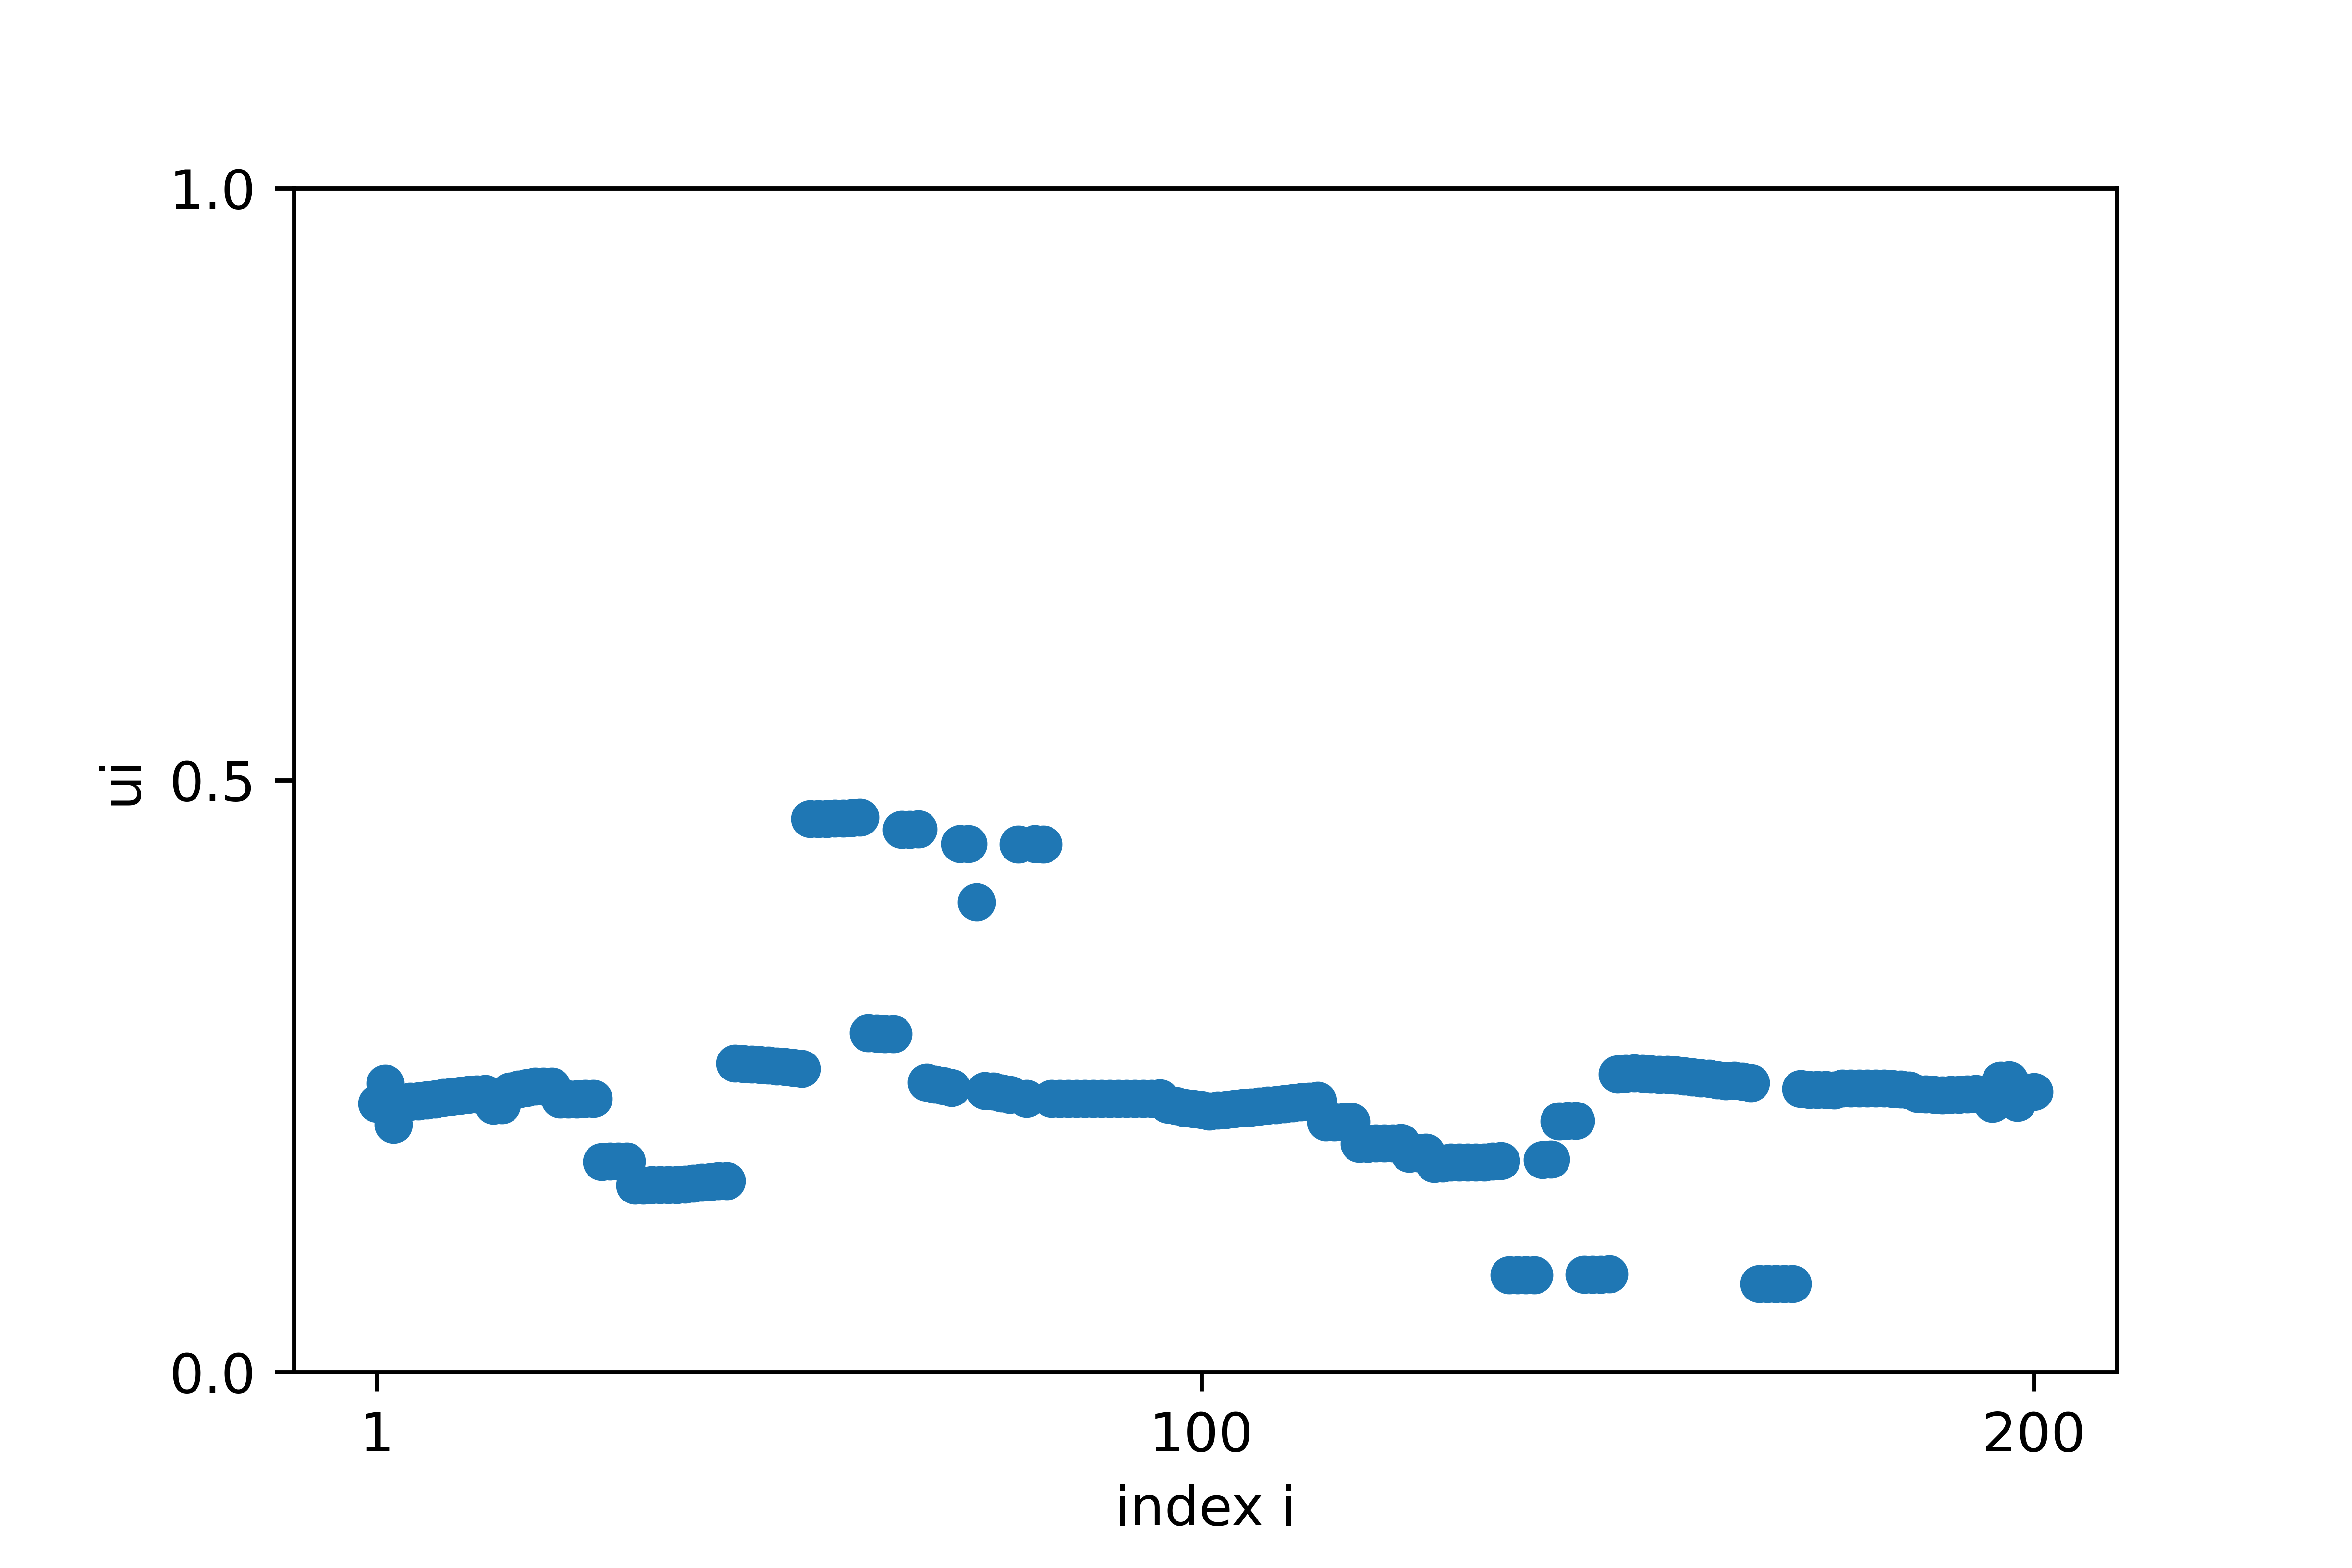
\includegraphics[width = \linewidth]{u_N=200_sigma=1.4_t=4000.png}
\caption{$t=4000$}
\end{subfigure}
\caption{Snapshots of the membrane potential $u_i$ at $t=1000$ and $t=4000$, for $N=200$, $\sigma=1.1$ and $r=0.35$.}
\label{1.4}
\end{figure}

\begin{figure}[H]
\centering
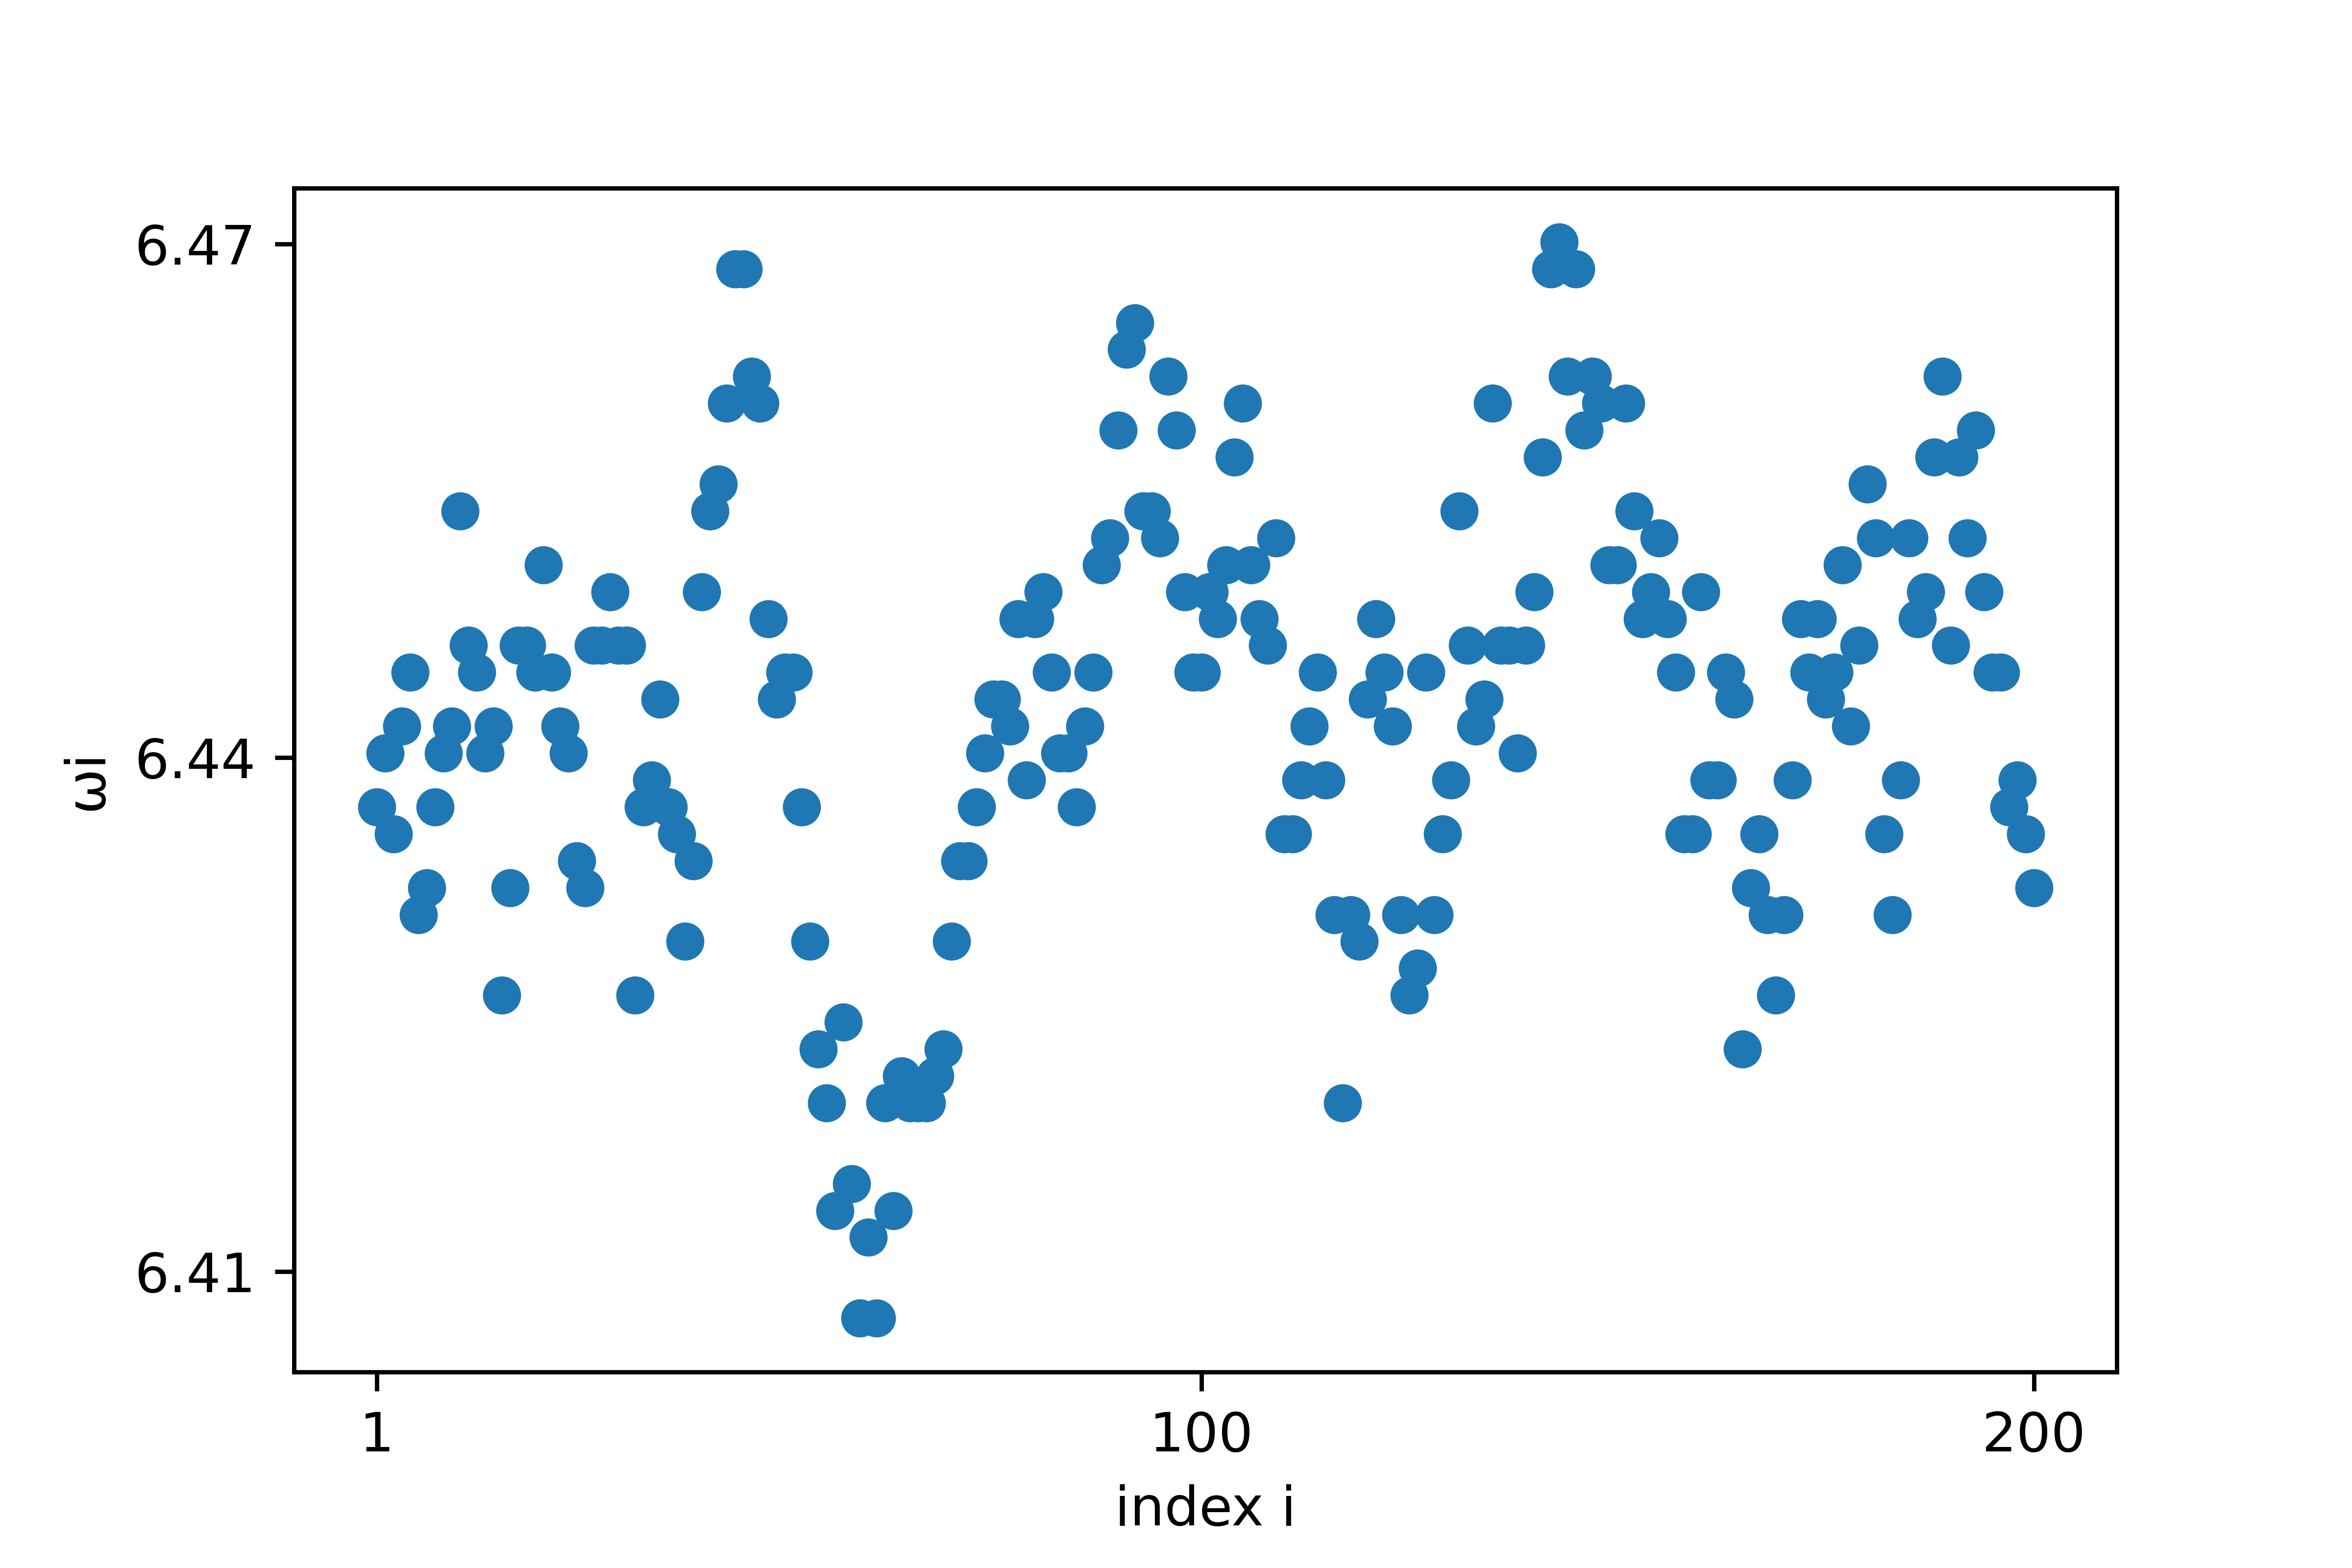
\includegraphics[width = 0.6 \textwidth]{w_N=200_sigma=1.4_t=4000.png}
\caption{Mean phase-velocity profile $\omega_i$ at $t=4000$, for $N=200$, $\sigma=1.1$ and $r=0.35$.}
\label{1.4omega}
\end{figure}

\subsection{Varying $\lambda$}
We now choose a set of parameters where a ``strong'' chimera is observed in the original $\lambda = 1$ LIF model. We slowly vary $\lambda$, in order to study how the chimera disintegrates due to the changing $\lambda$. For $N=150$, $r=0.4$ and $\sigma = 0.7$, the chimera disintegrates almost completely at around $\lambda = 0.95$. In Fig. (\ref{vslmd}), we see how $\Delta \omega$ changes when $\lambda$ is varied. Already at $\lambda=0.95$, $\Delta \omega$ drops to $\Delta \omega  \approx 0.04$. In Fig. (\ref{uivslmd}), snapshots of the potential $u_i$ are shown. The respective phase-velocity profiles $\omega_i$ are shown in Fig. (\ref{uivslmd2}).

\begin{figure}[H]
\centering
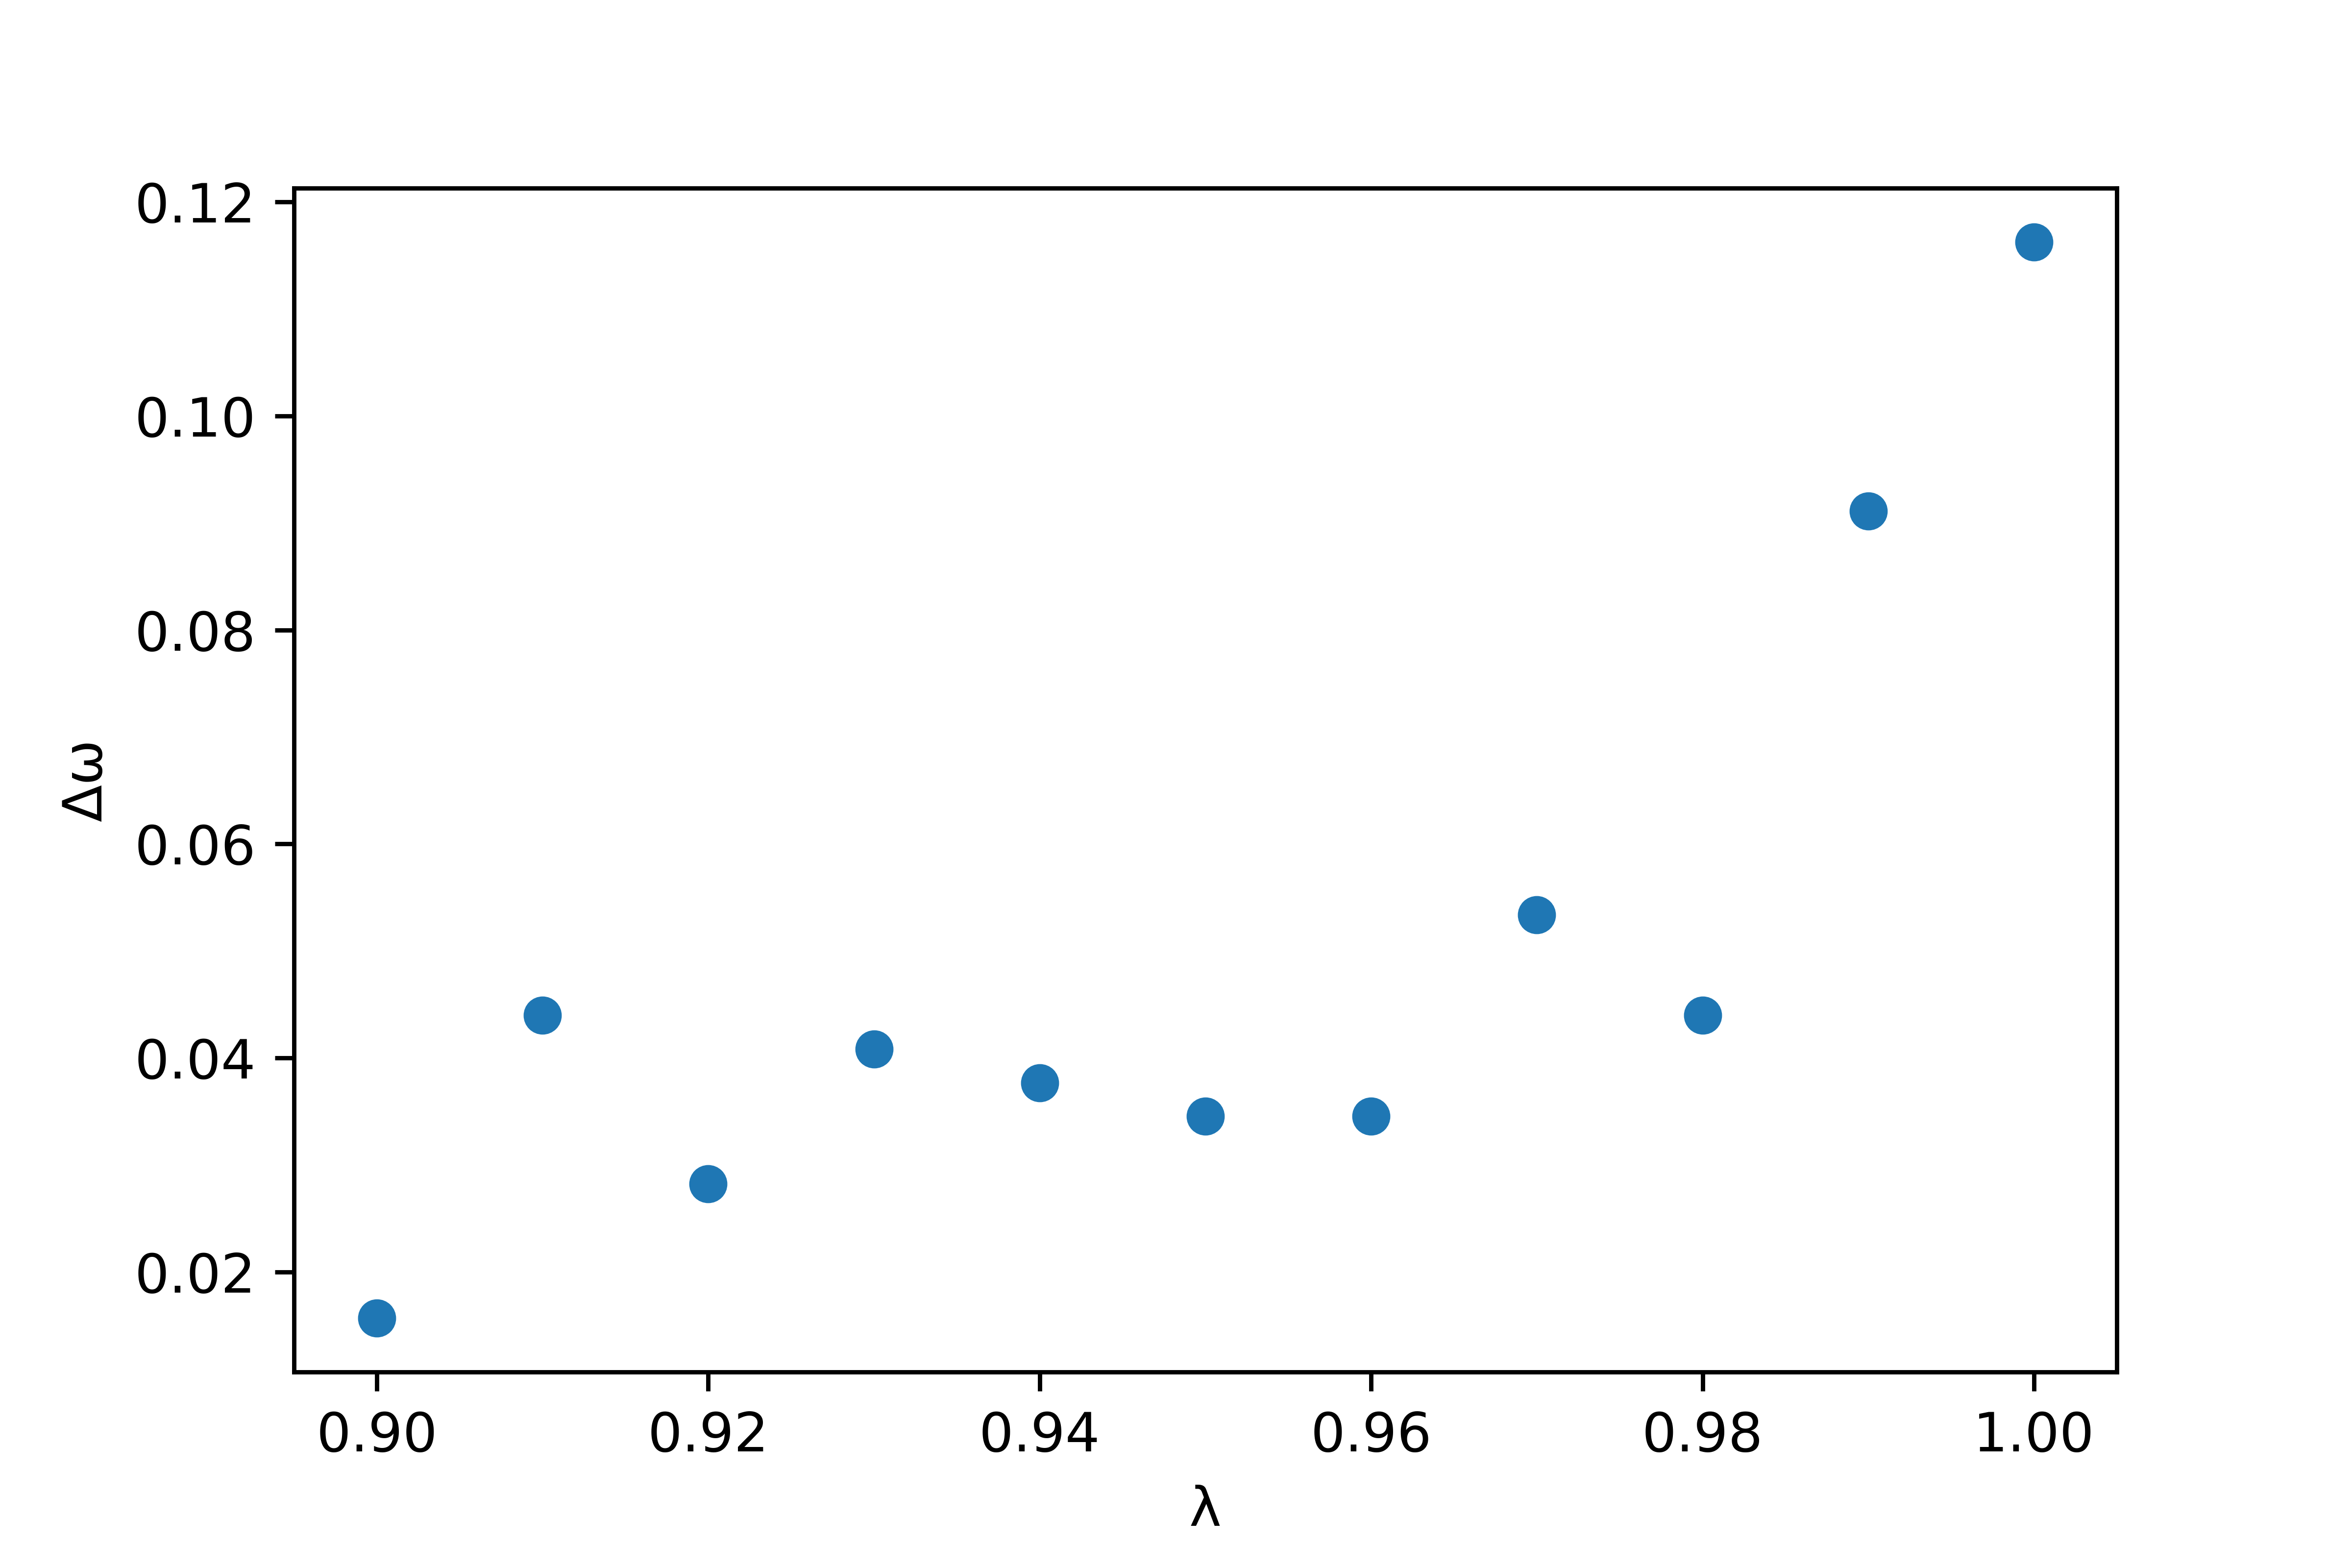
\includegraphics[width = 0.6 \textwidth]{deltawvslmd.png}
\caption{$\Delta \omega = \omega_{\text{max}}-\omega_{\text{min}}$ with varying $\lambda$.}
\label{vslmd}
\end{figure}

\begin{figure}[H]
\begin{subfigure}{.32\textwidth}
  \centering
  % include first image
  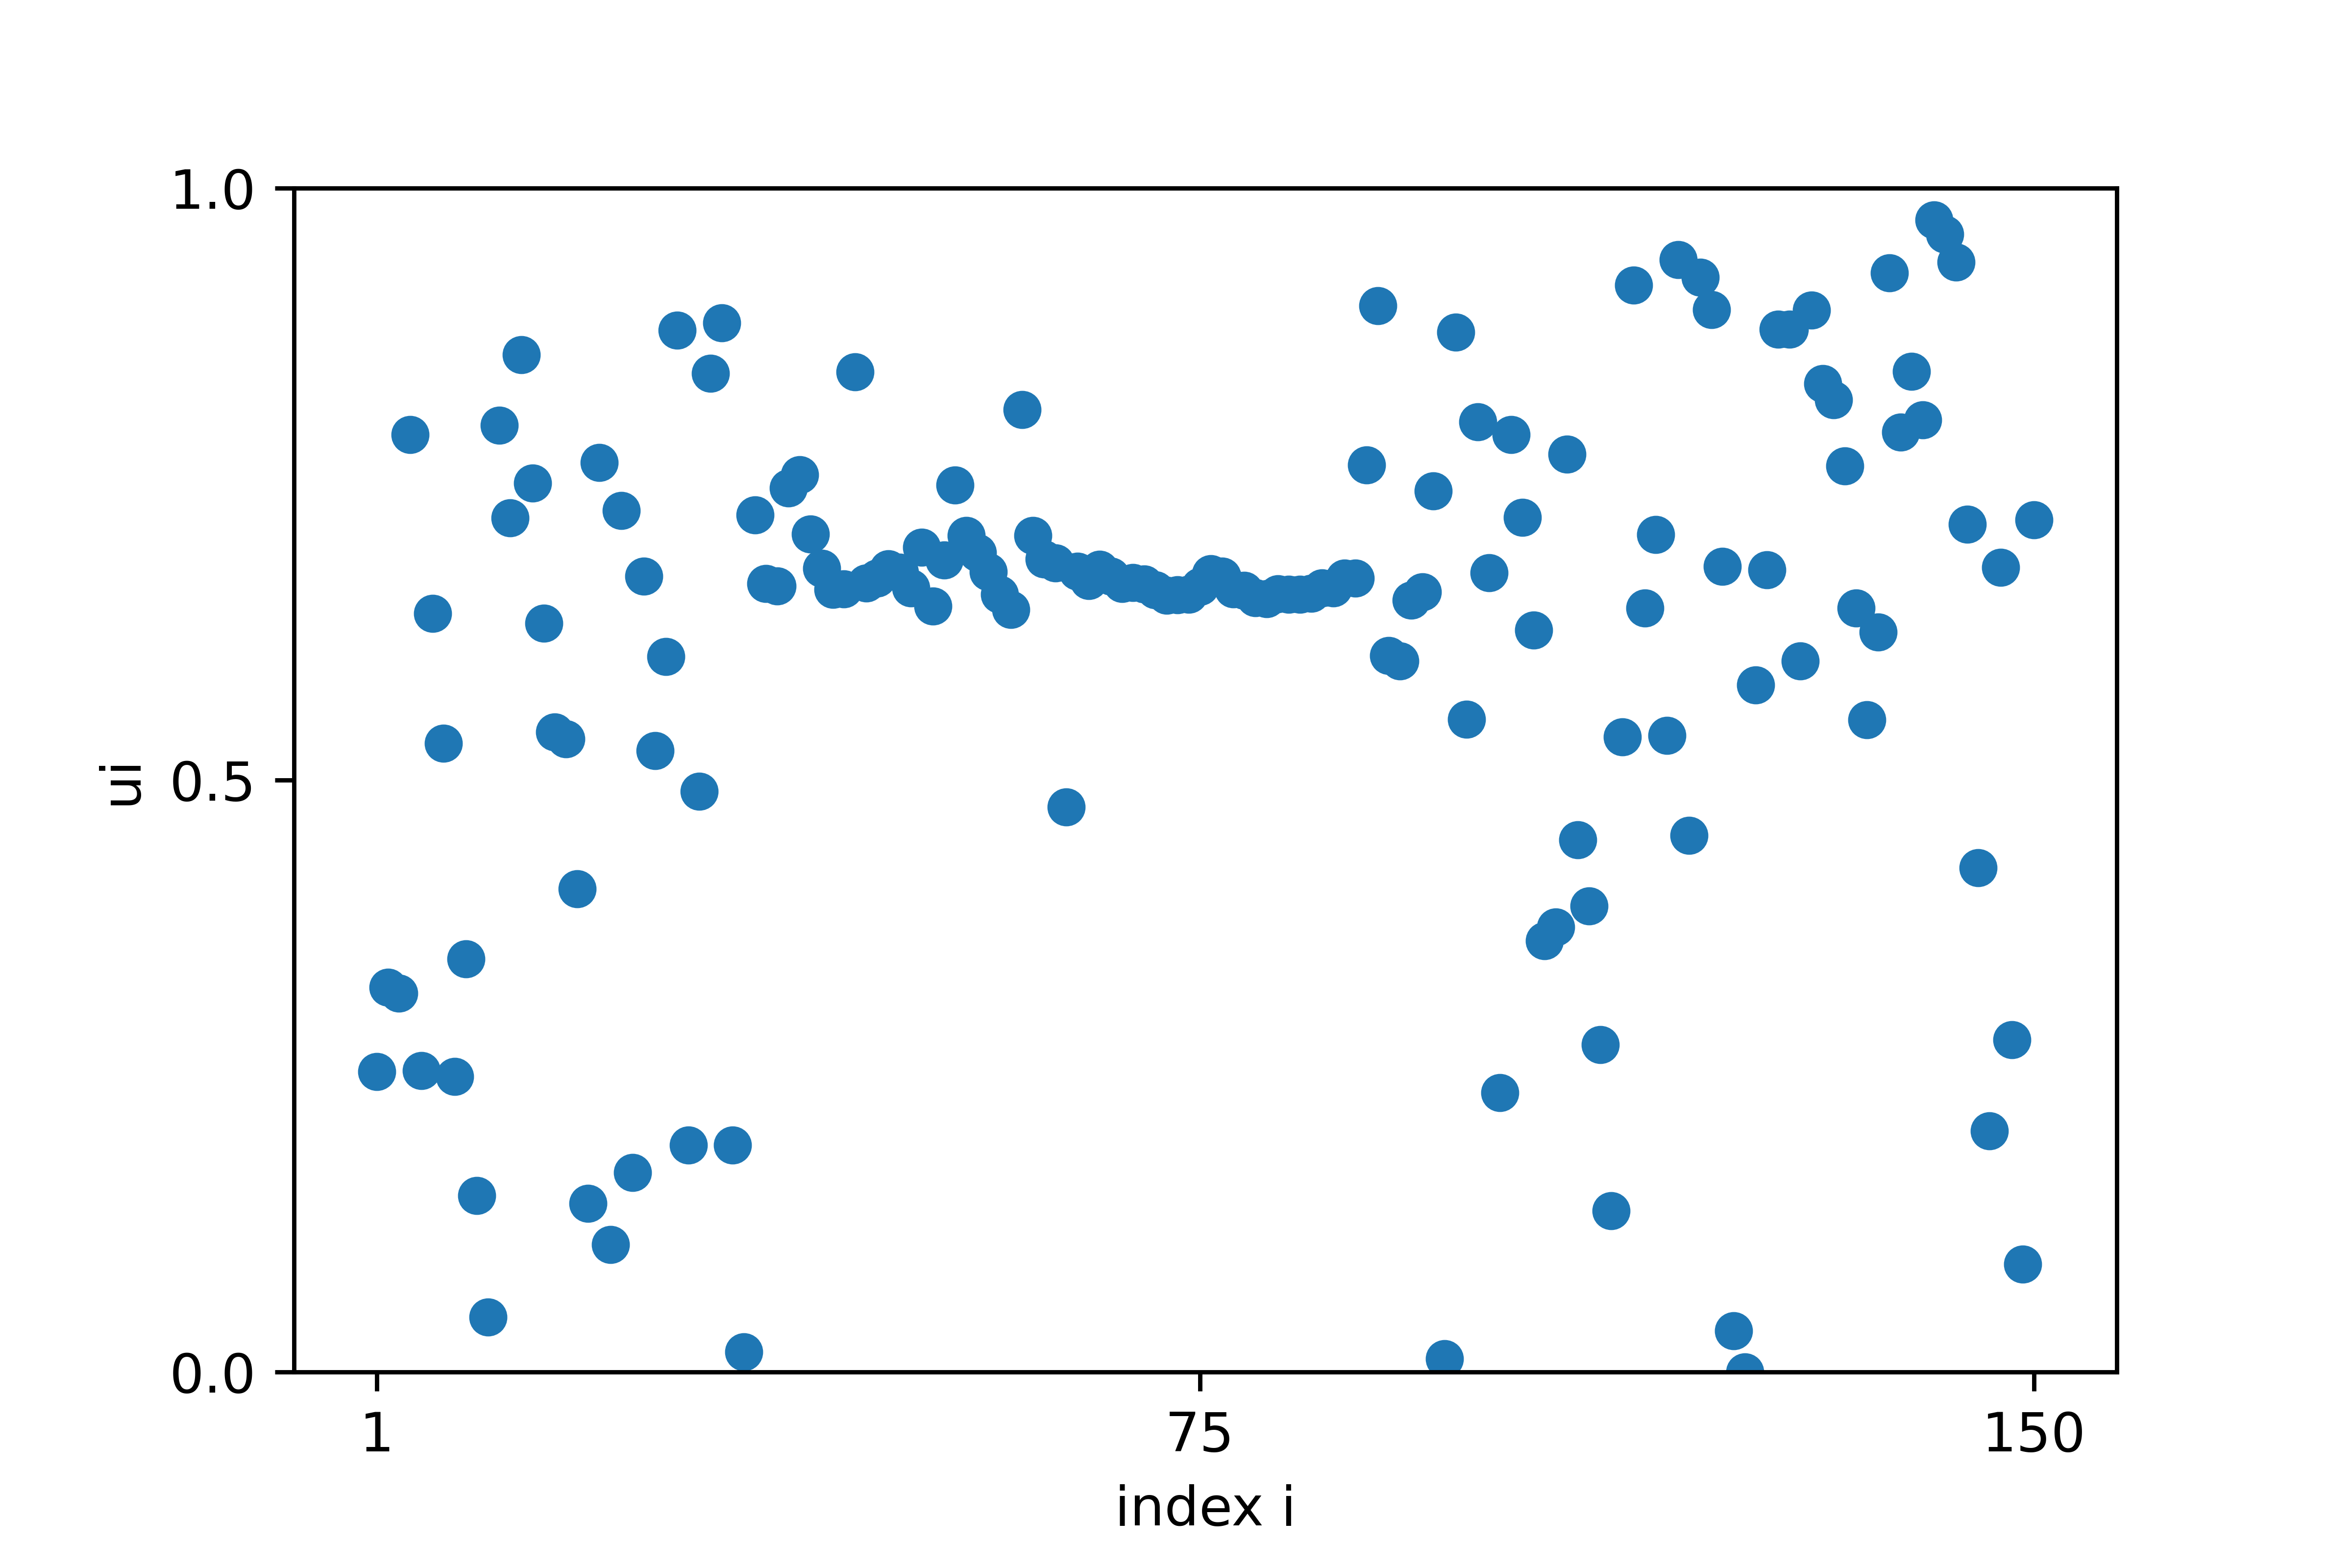
\includegraphics[width=1\linewidth]{u_lambda=1.0_t=2000.png}  
  \caption{$\lambda=1.00$}
\end{subfigure}
\hfill
\begin{subfigure}{.32\textwidth}
  \centering
  % include second image
  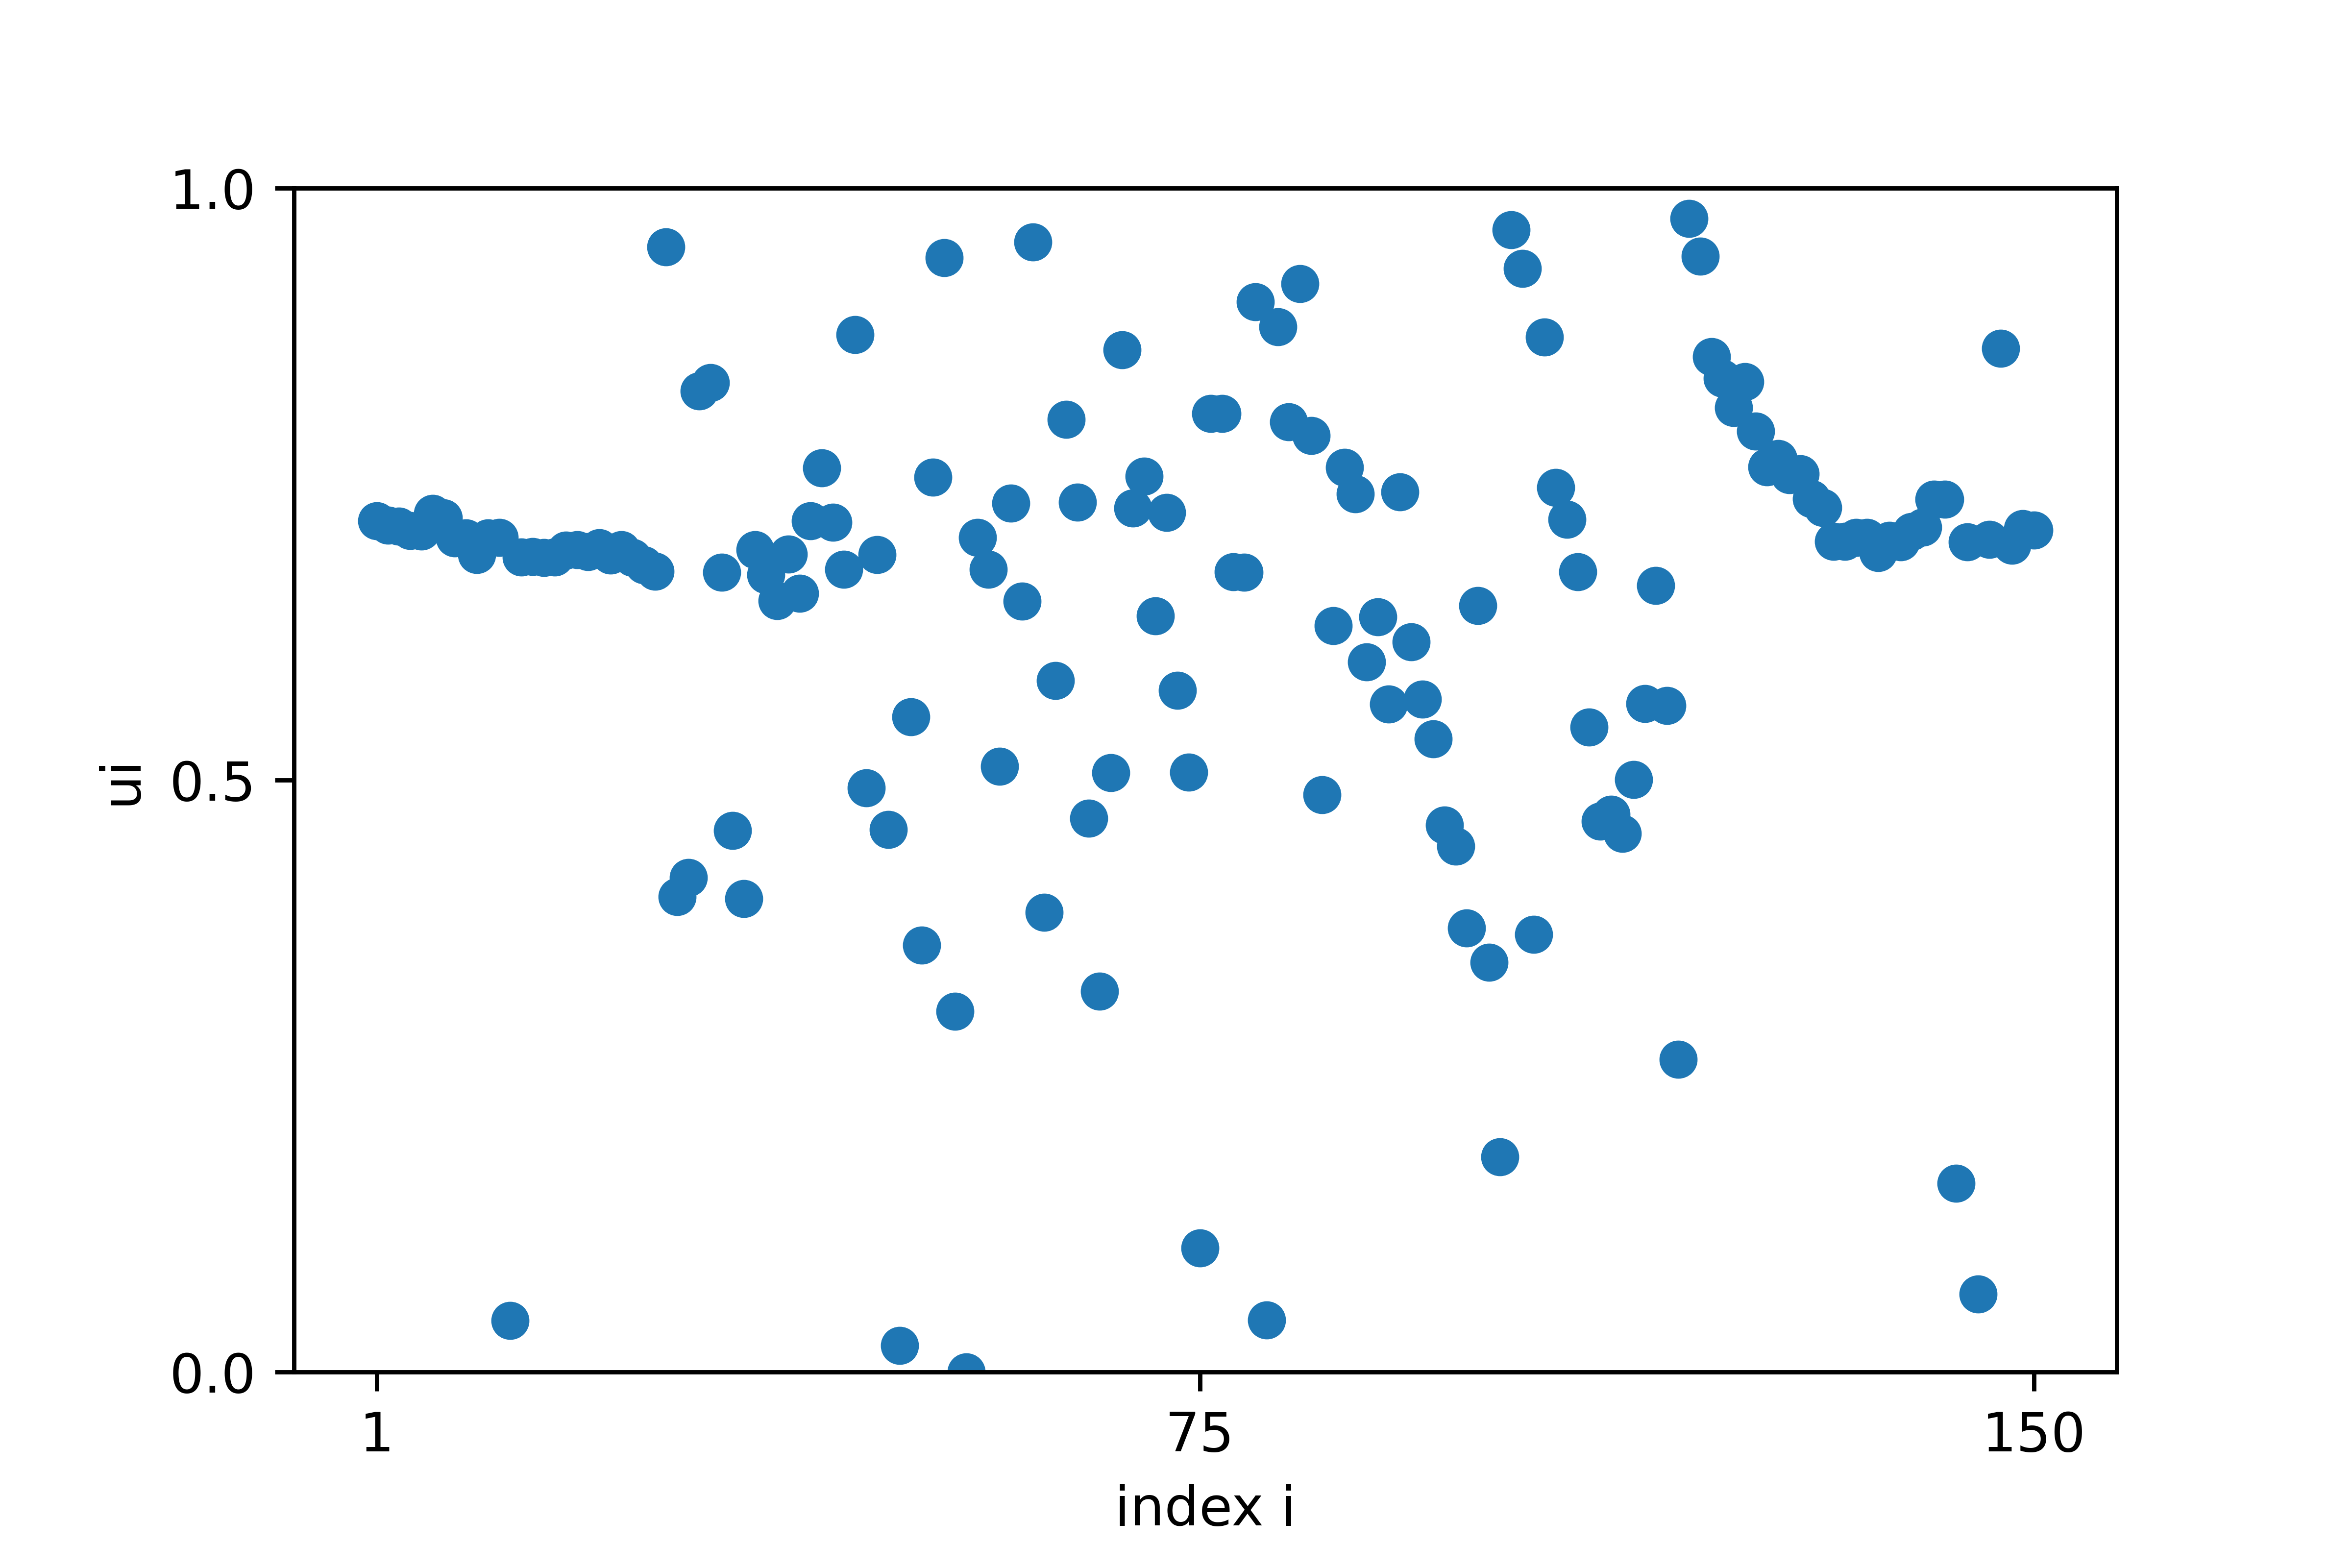
\includegraphics[width=1\linewidth]{u_lambda=0.99_t=2000.png}  
  \caption{$\lambda=0.99$}
\end{subfigure}
\hfill
\begin{subfigure}{.32\textwidth}
  \centering
  % include first image
  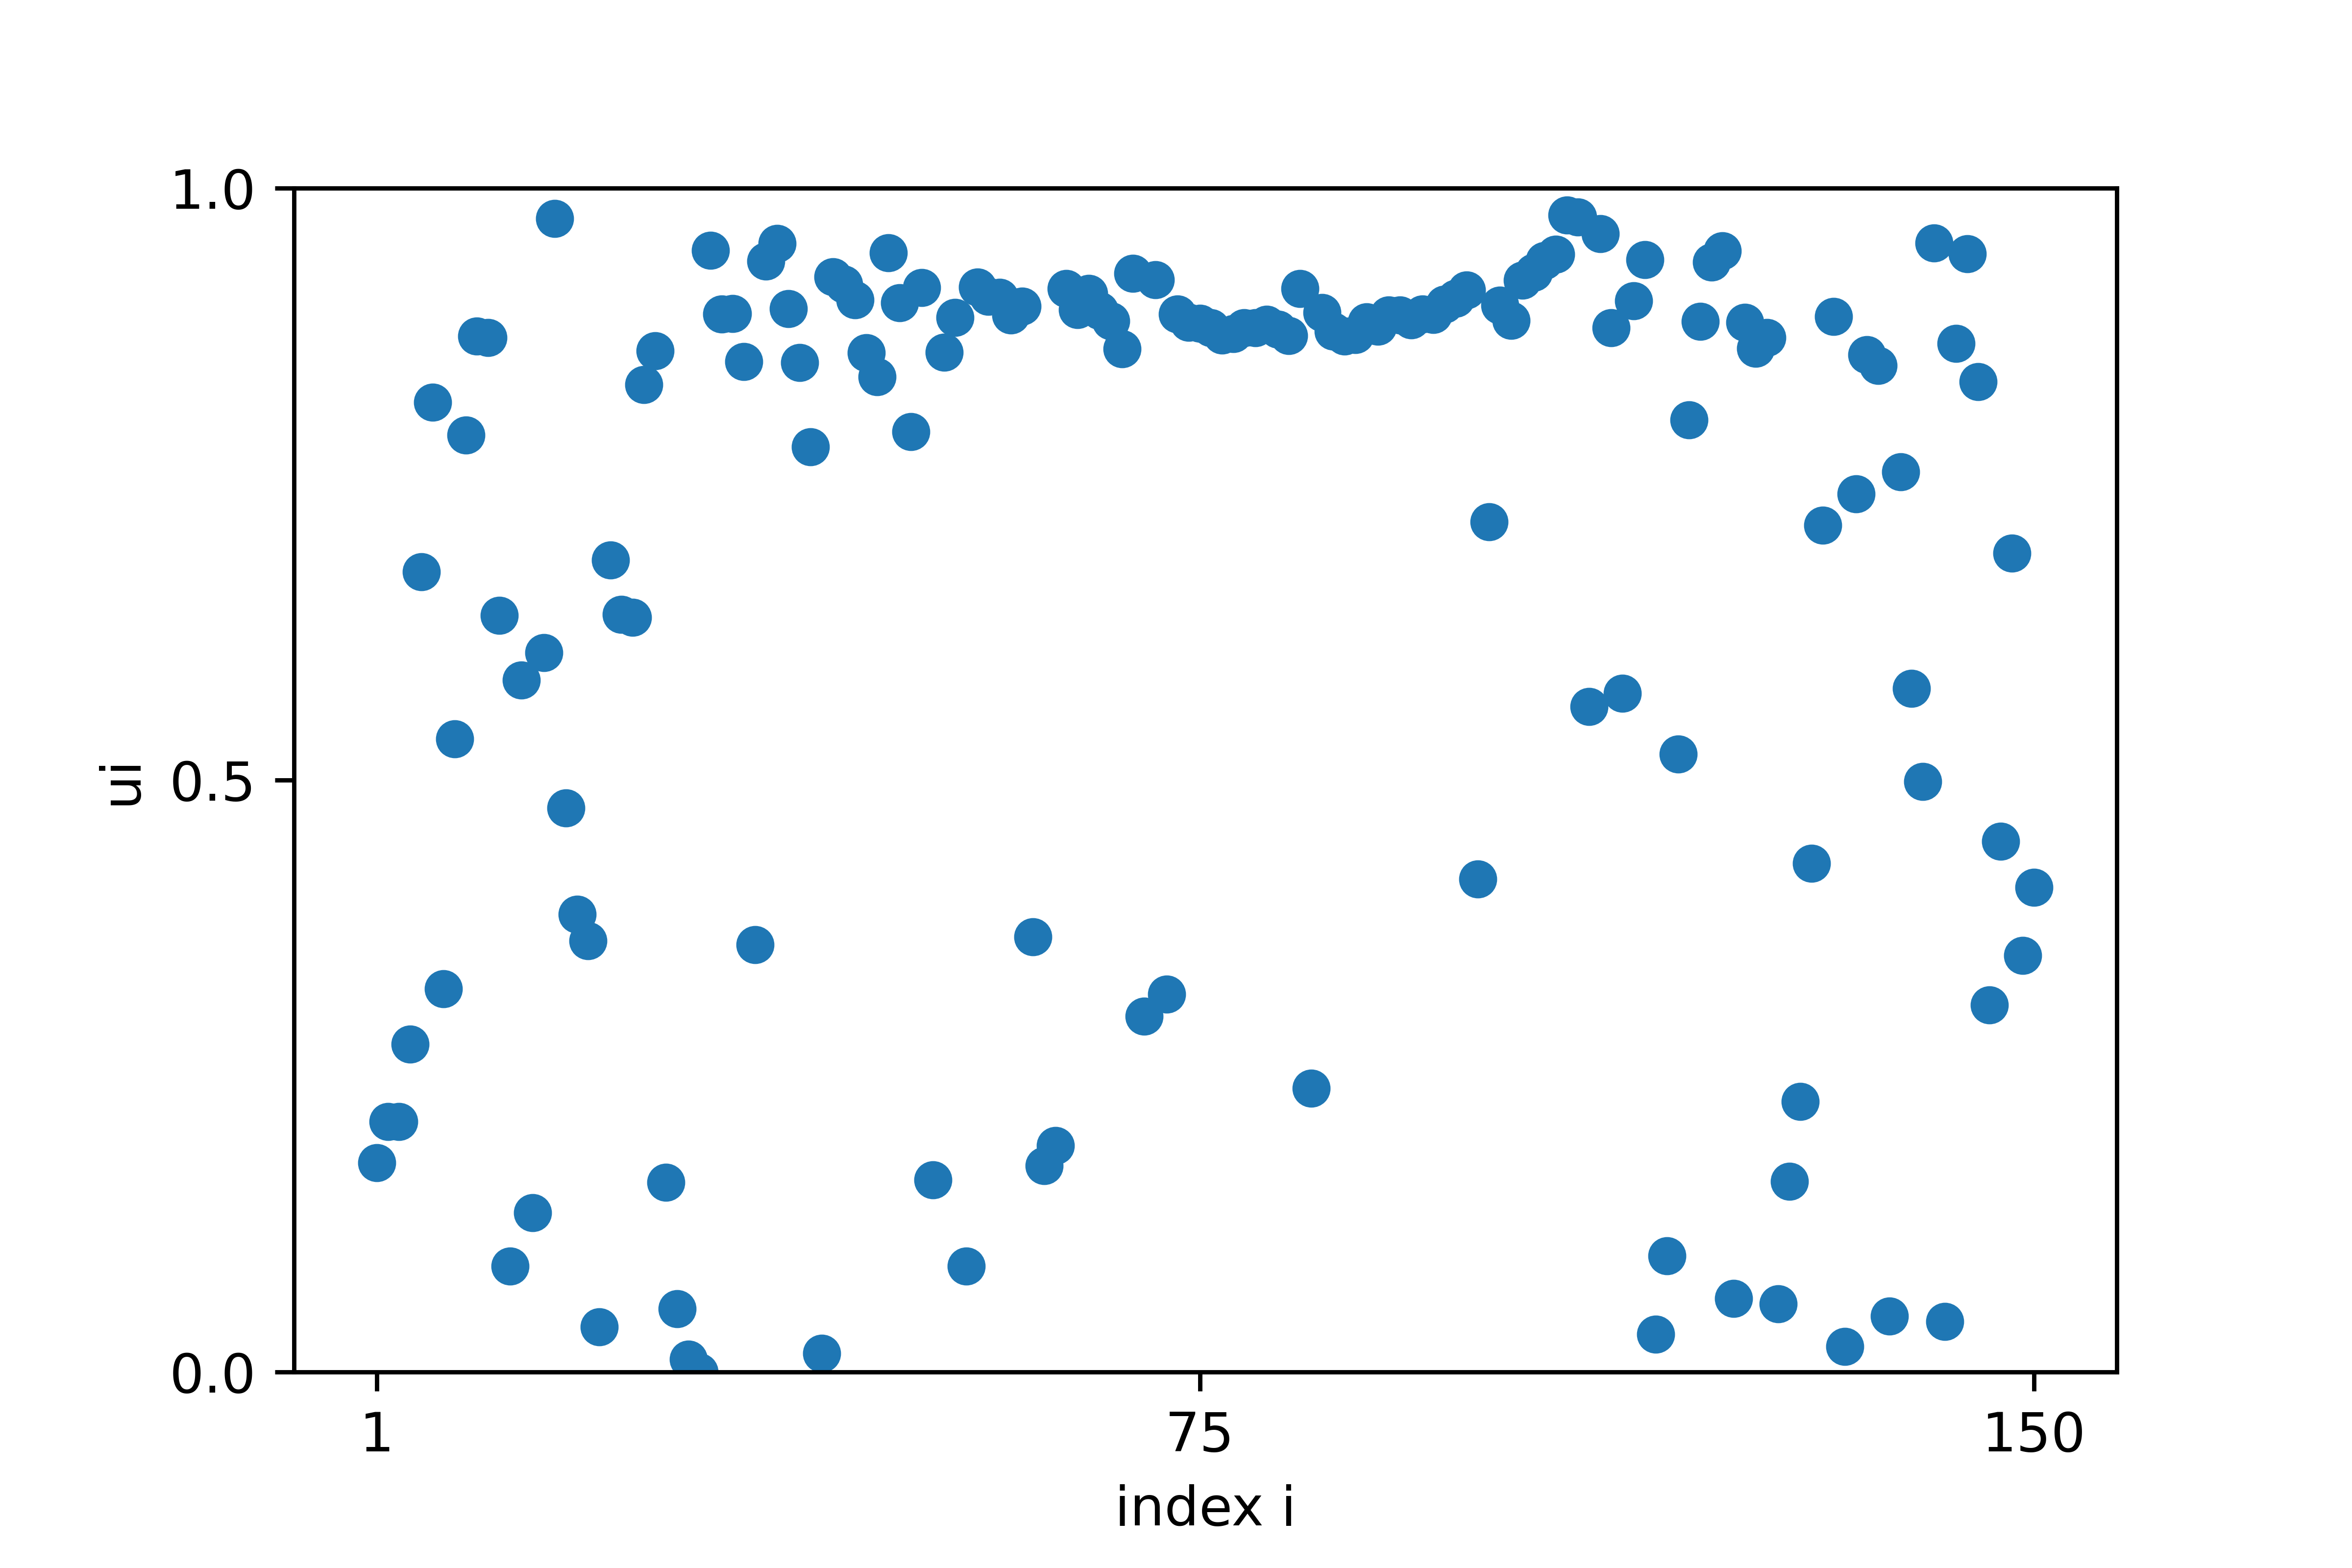
\includegraphics[width=1\linewidth]{u_lambda=0.98_t=2000}  
  \caption{$\lambda=0.98$}
\end{subfigure}
\begin{subfigure}{.32\textwidth}
  \centering
  % include first image
  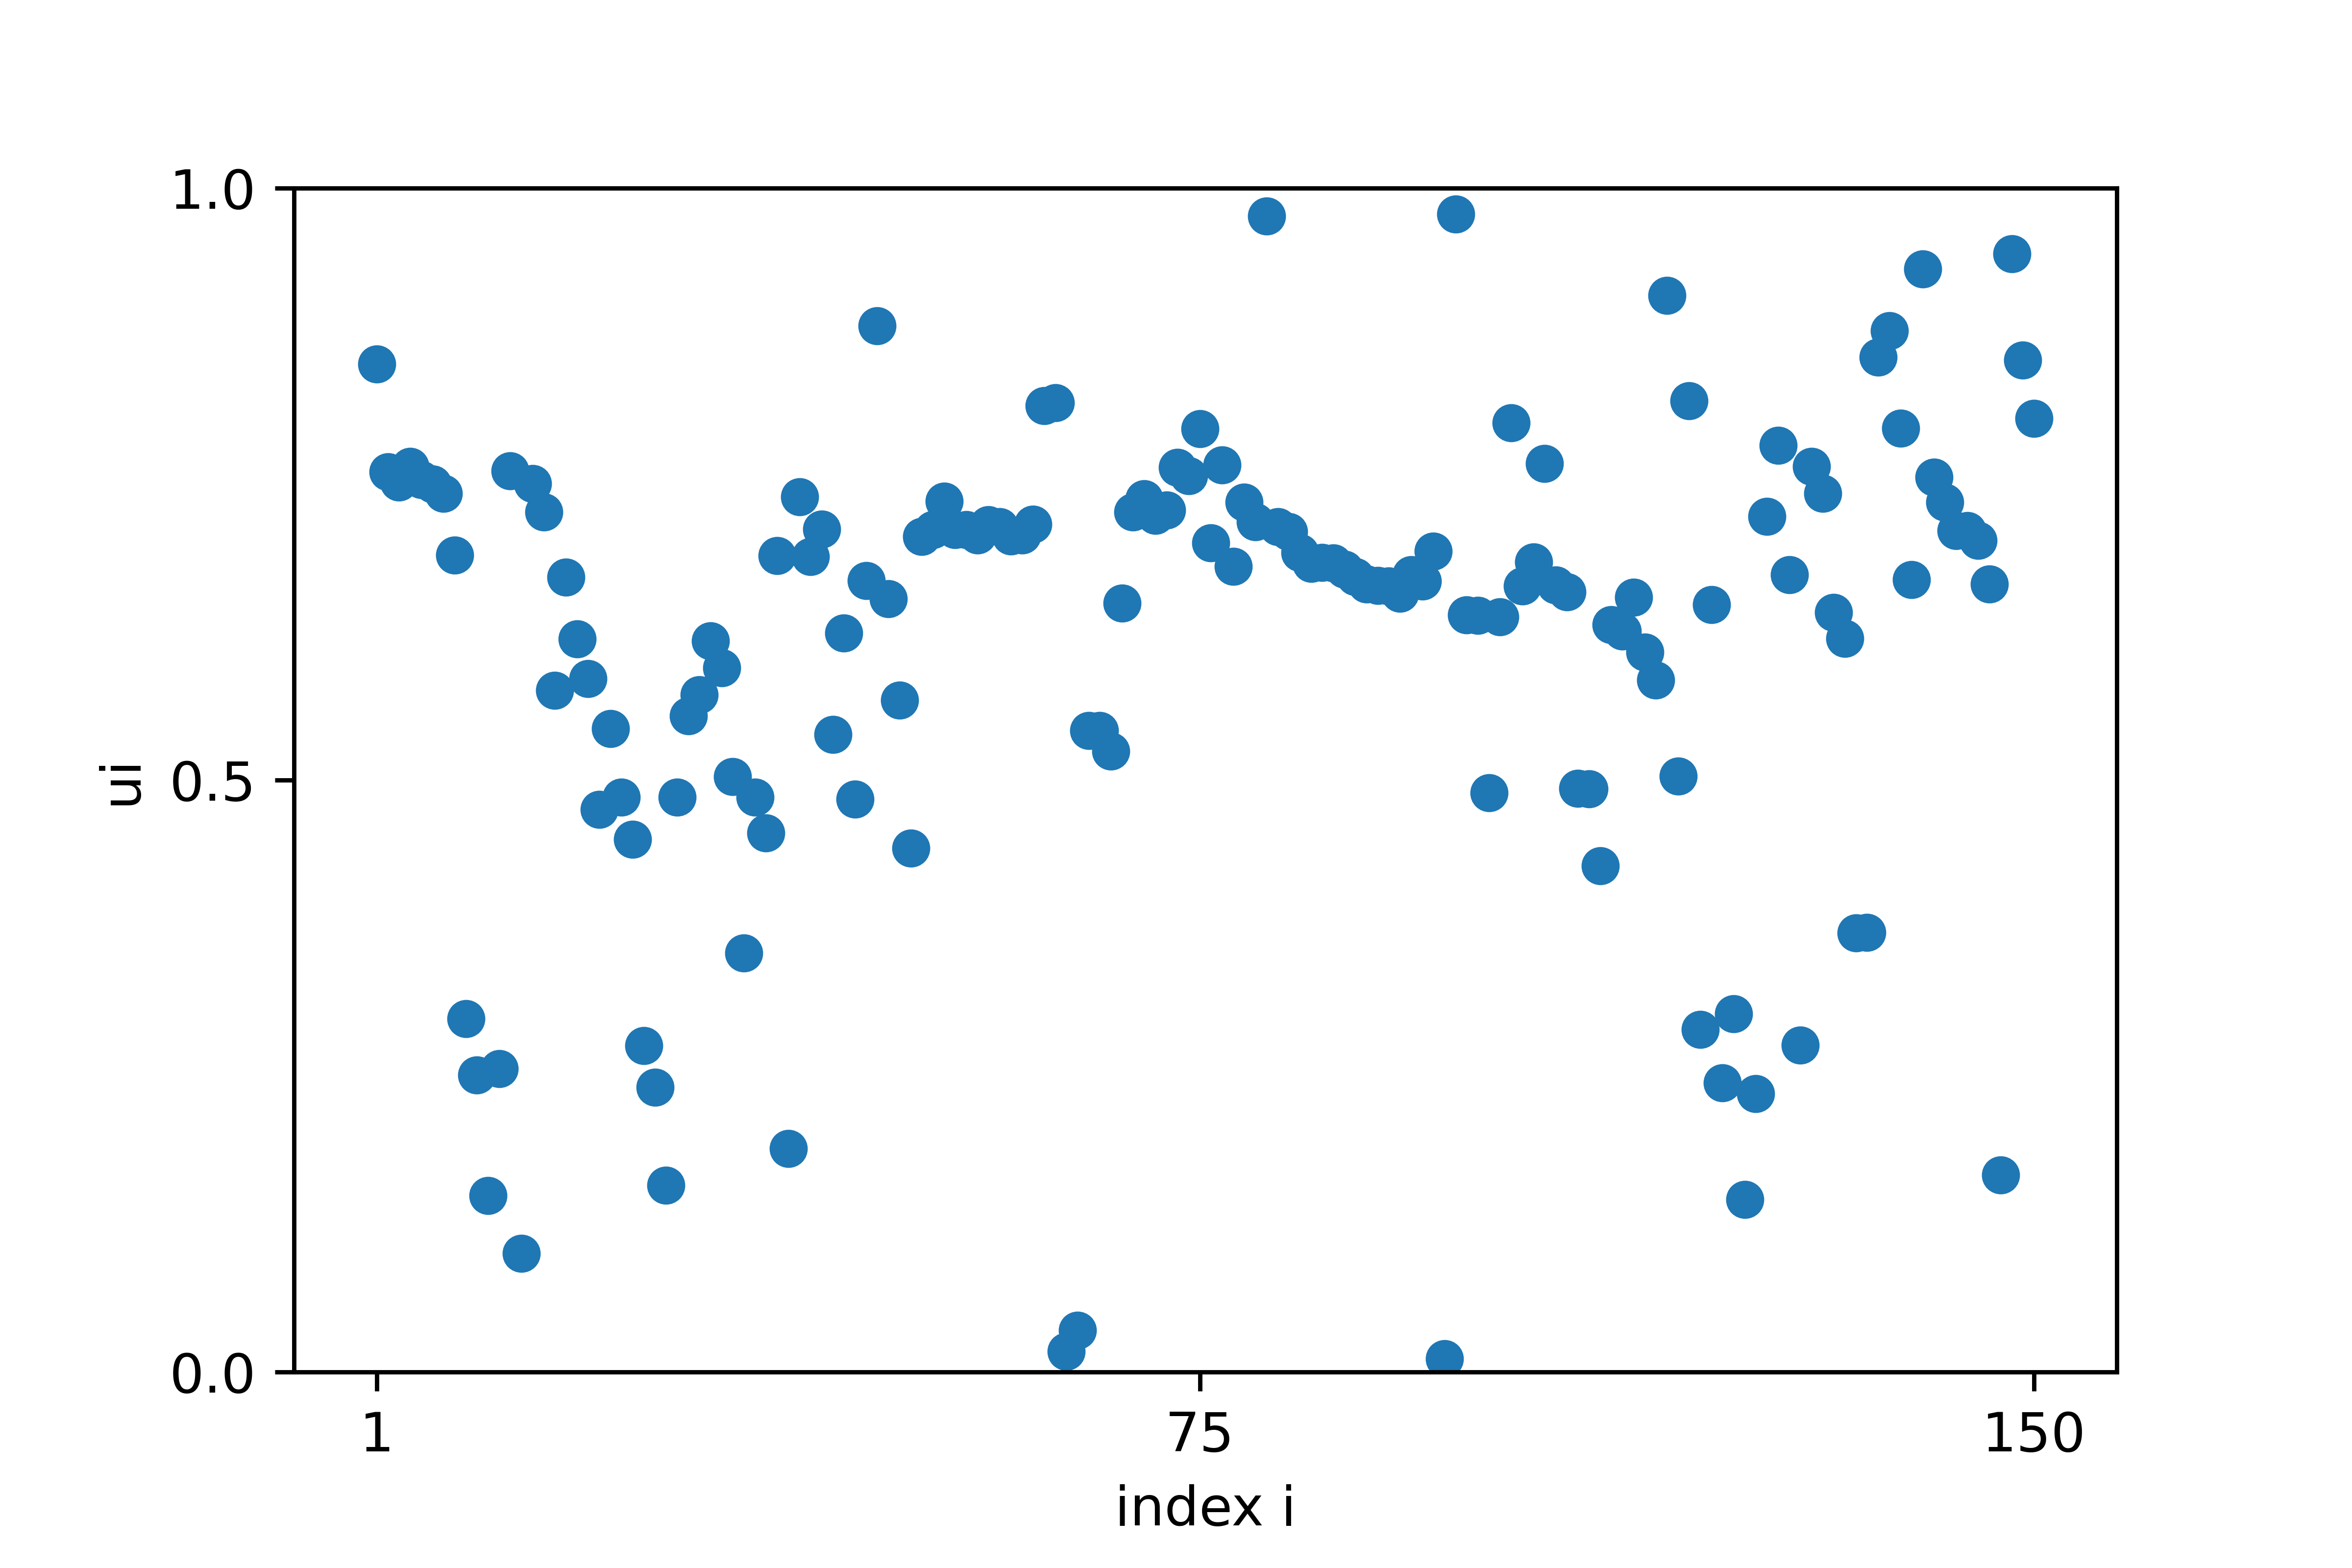
\includegraphics[width=1\linewidth]{u_lambda=0.97_t=2000.png}  
  \caption{$\lambda=0.97$}
\end{subfigure}
\hfill
\begin{subfigure}{.32\textwidth}
  \centering
  % include first image
  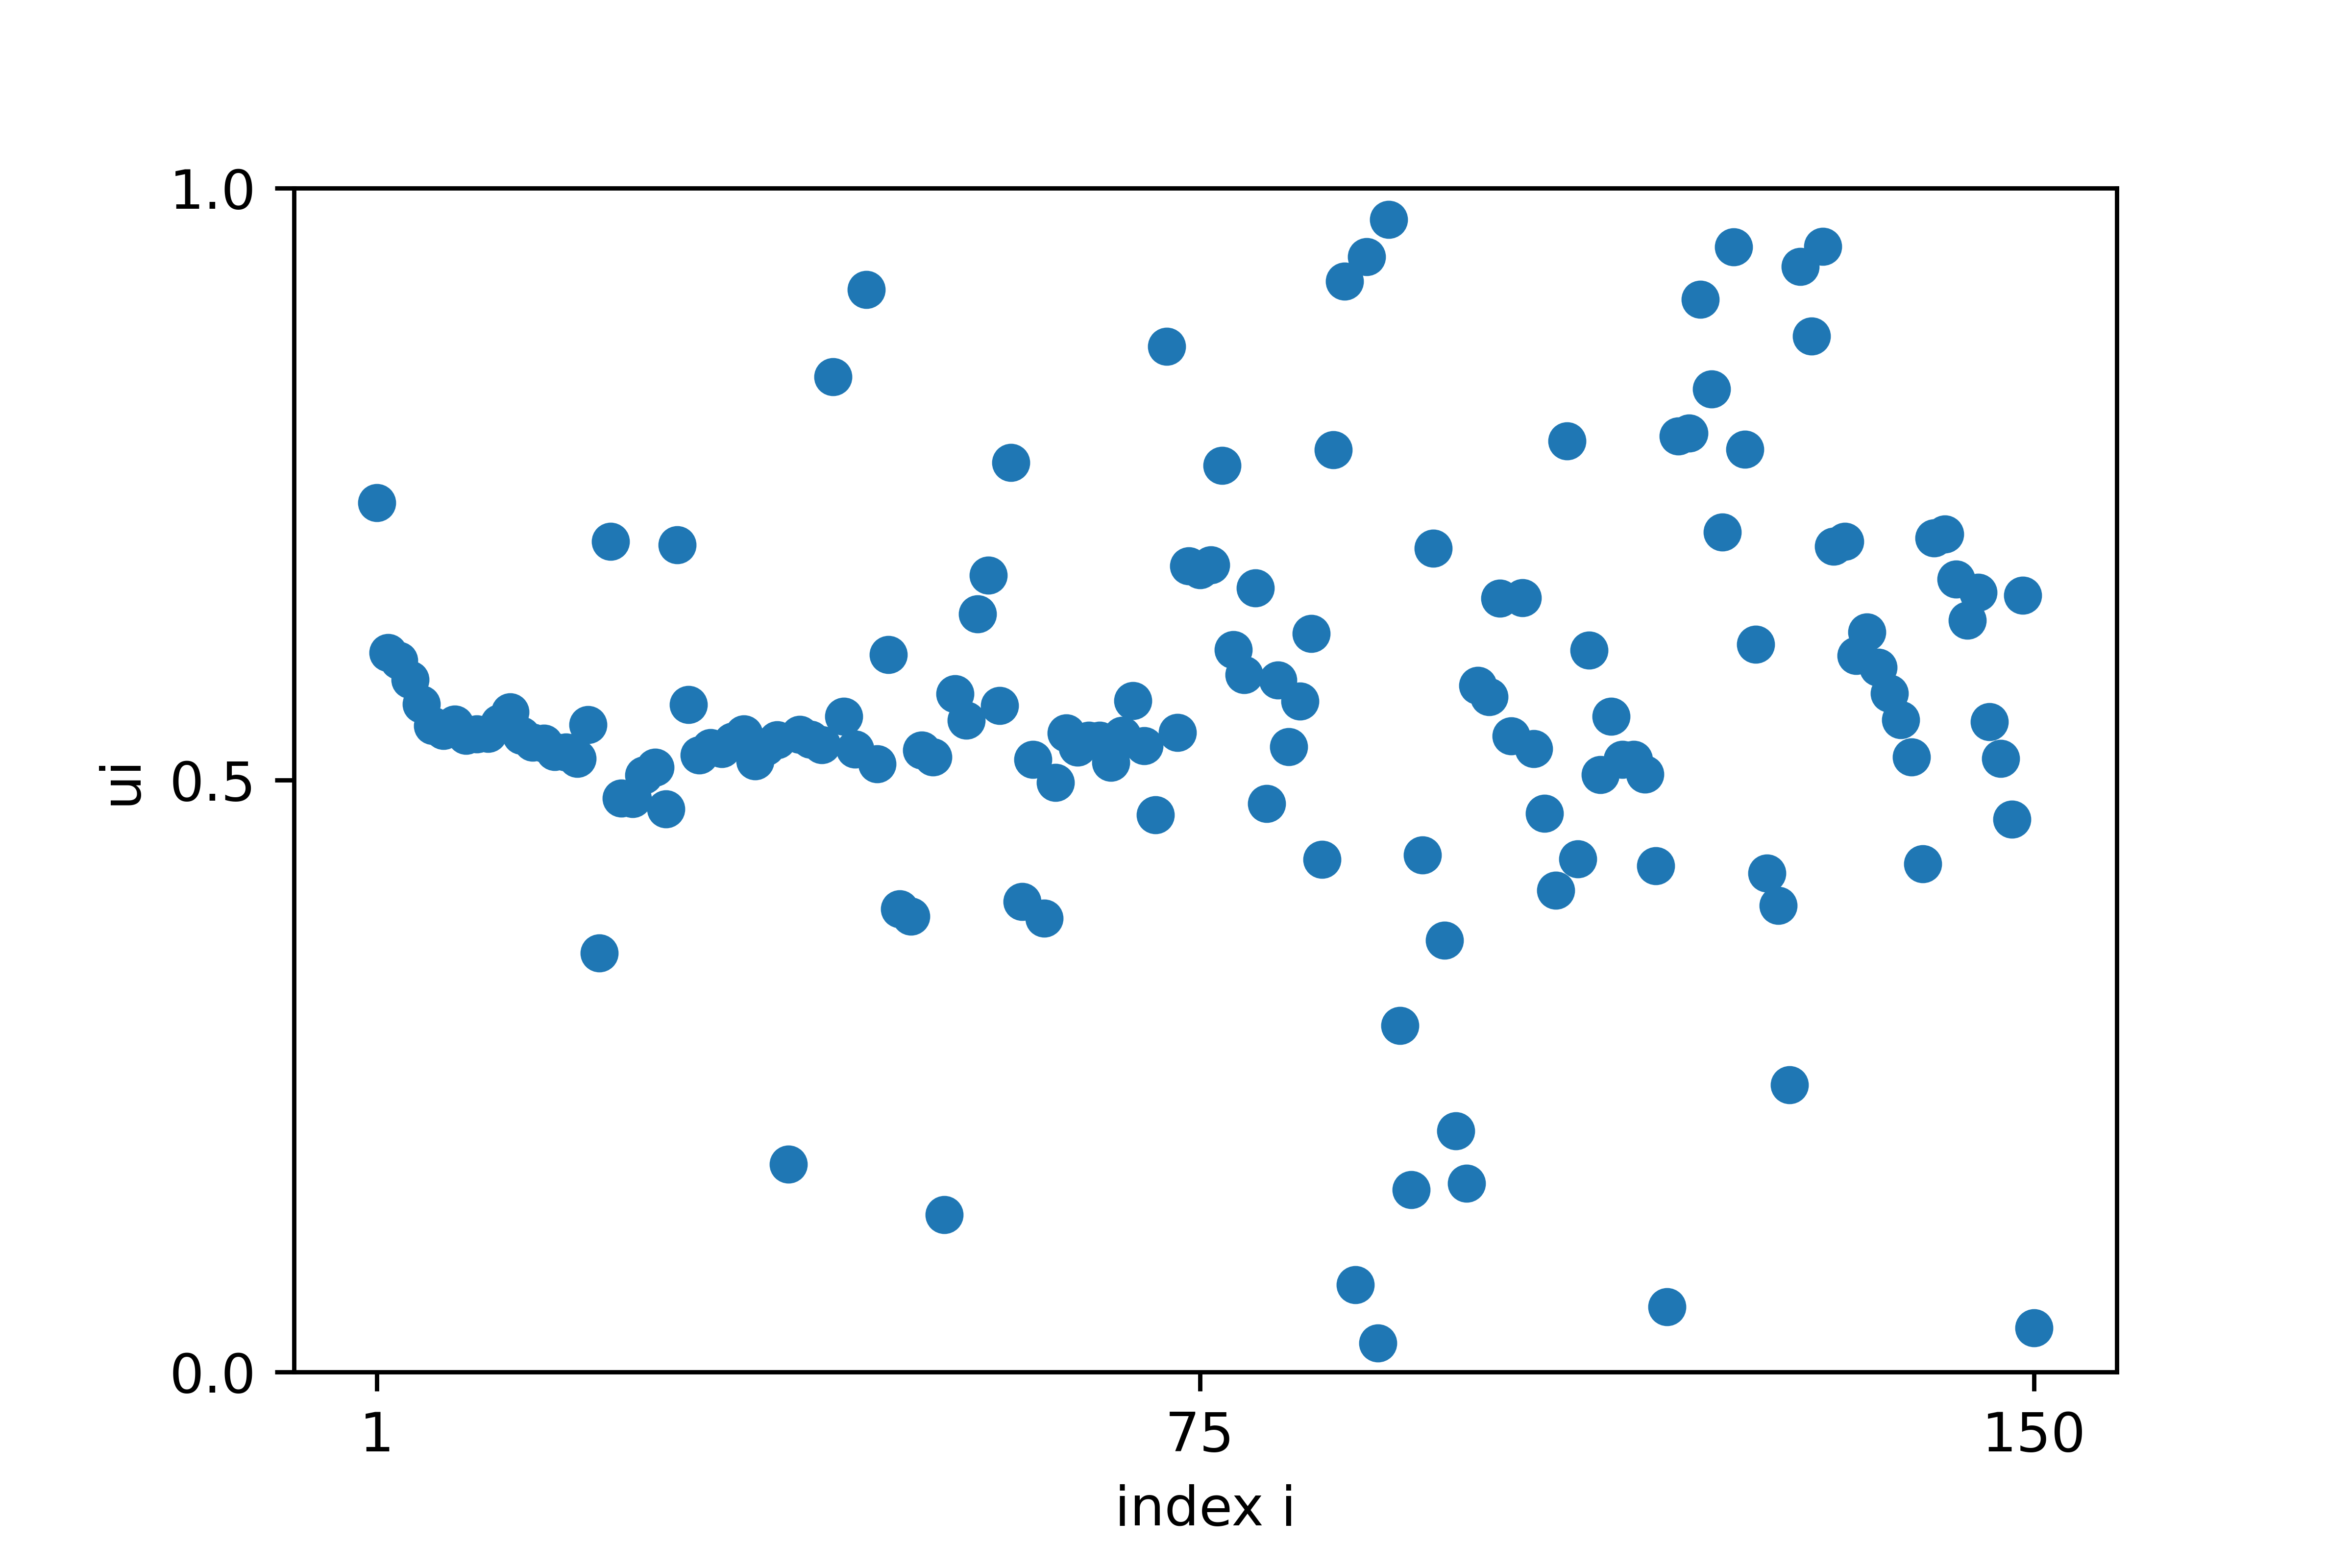
\includegraphics[width=1\linewidth]{u_lambda=0.96_t=2000.png}  
  \caption{$\lambda=0.96$}
\end{subfigure}
\hfill
\begin{subfigure}{.32\textwidth}
  \centering
  % include first image
  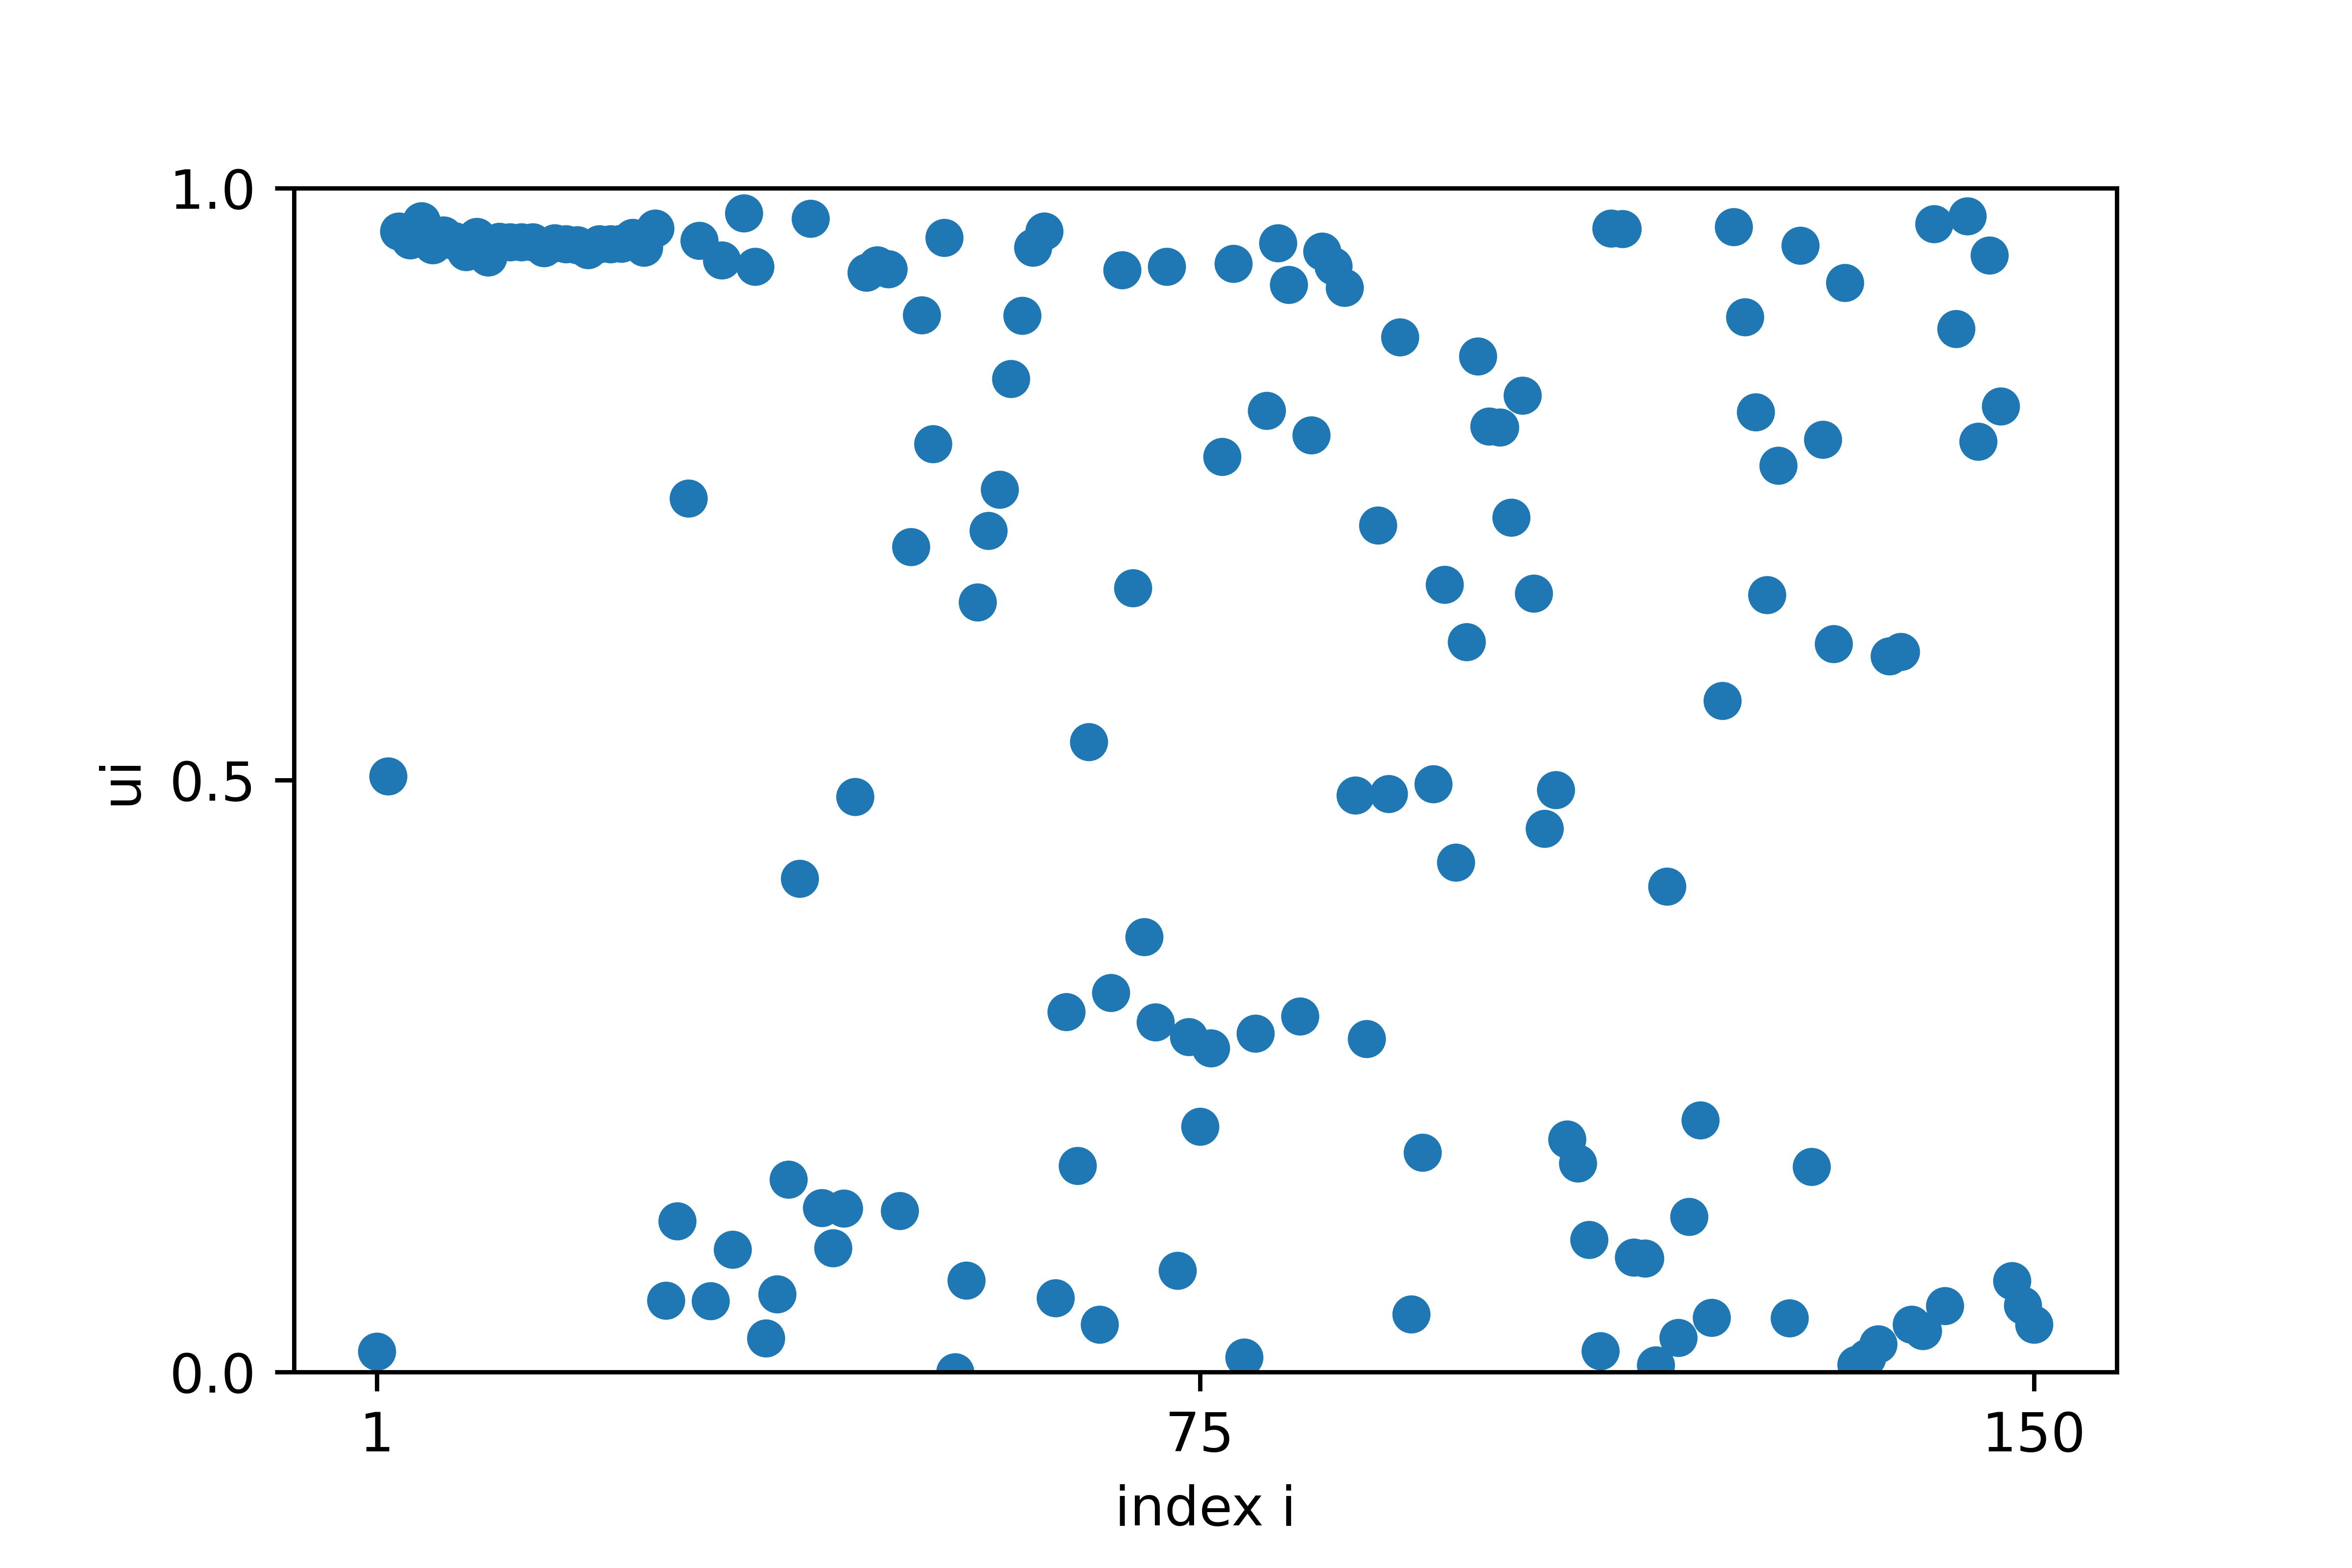
\includegraphics[width=1\linewidth]{u_lambda=0.95_t=2000.png}  
  \caption{$\lambda=0.95$}
\end{subfigure}

\begin{subfigure}{.32\textwidth}
  \centering
  % include first image
  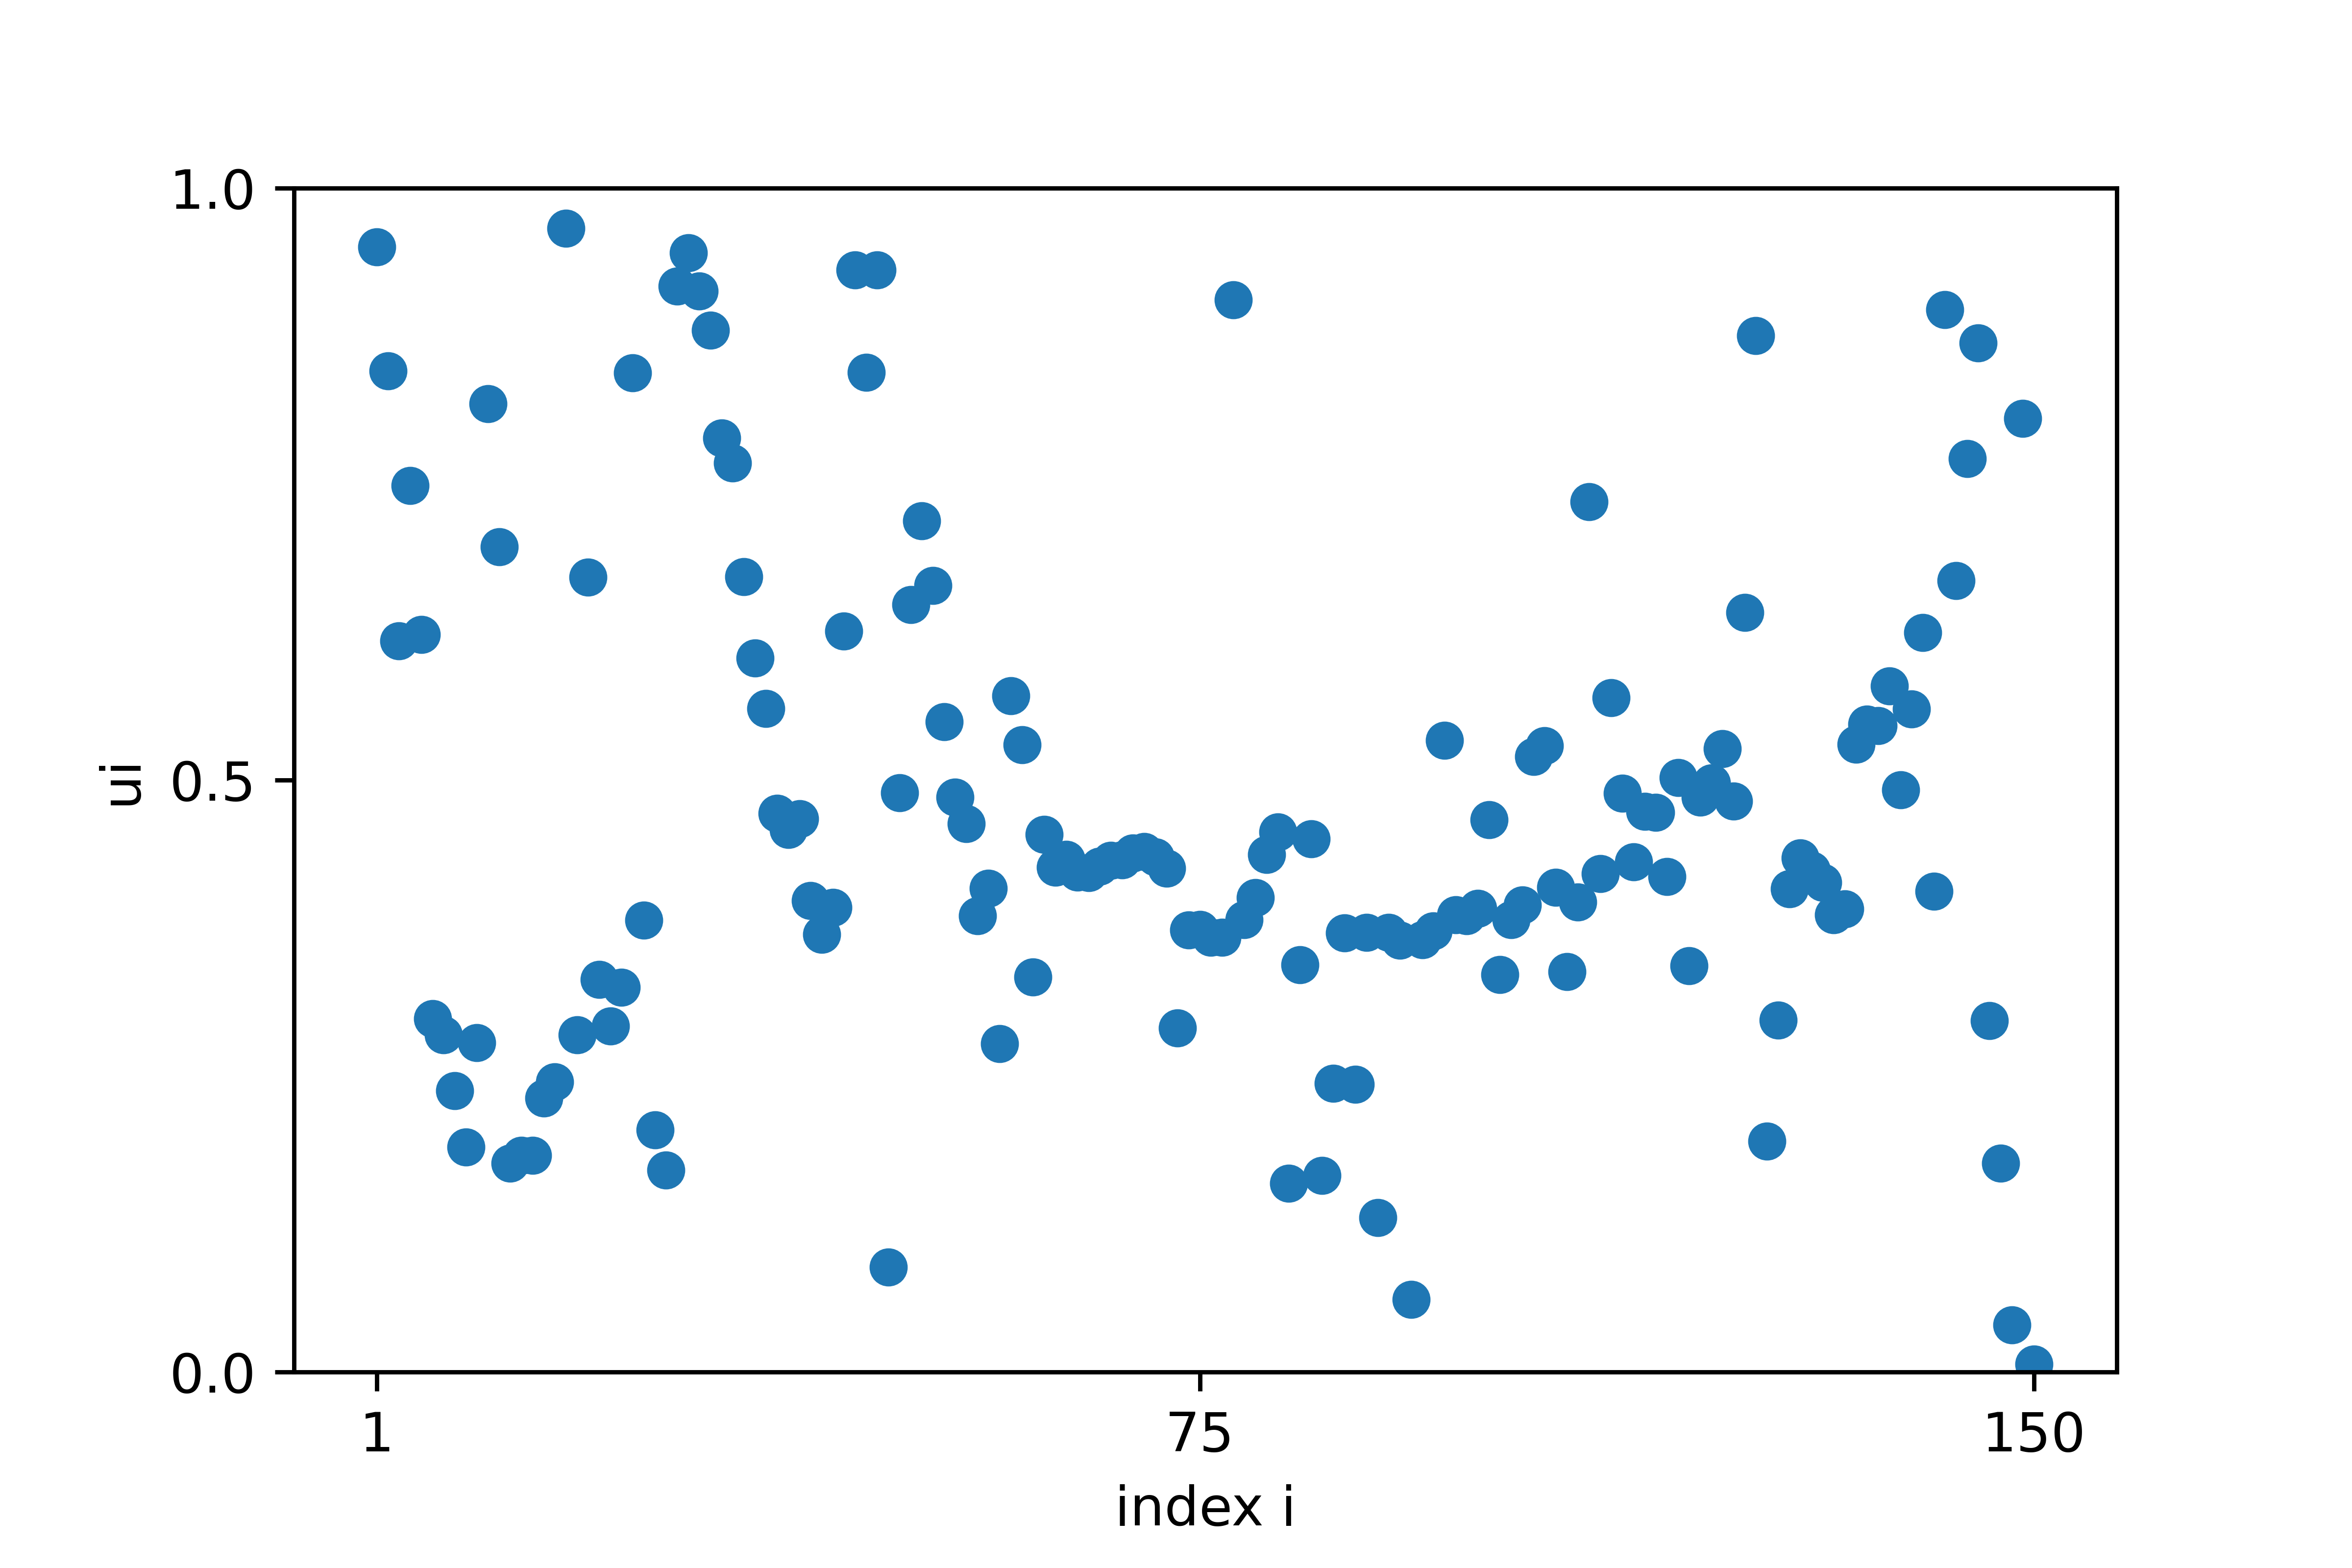
\includegraphics[width=1\linewidth]{u_lambda=0.94_t=2000.png}  
  \caption{$\lambda=0.94$}
\end{subfigure}
\hfill
\begin{subfigure}{.32\textwidth}
  \centering
  % include second image
  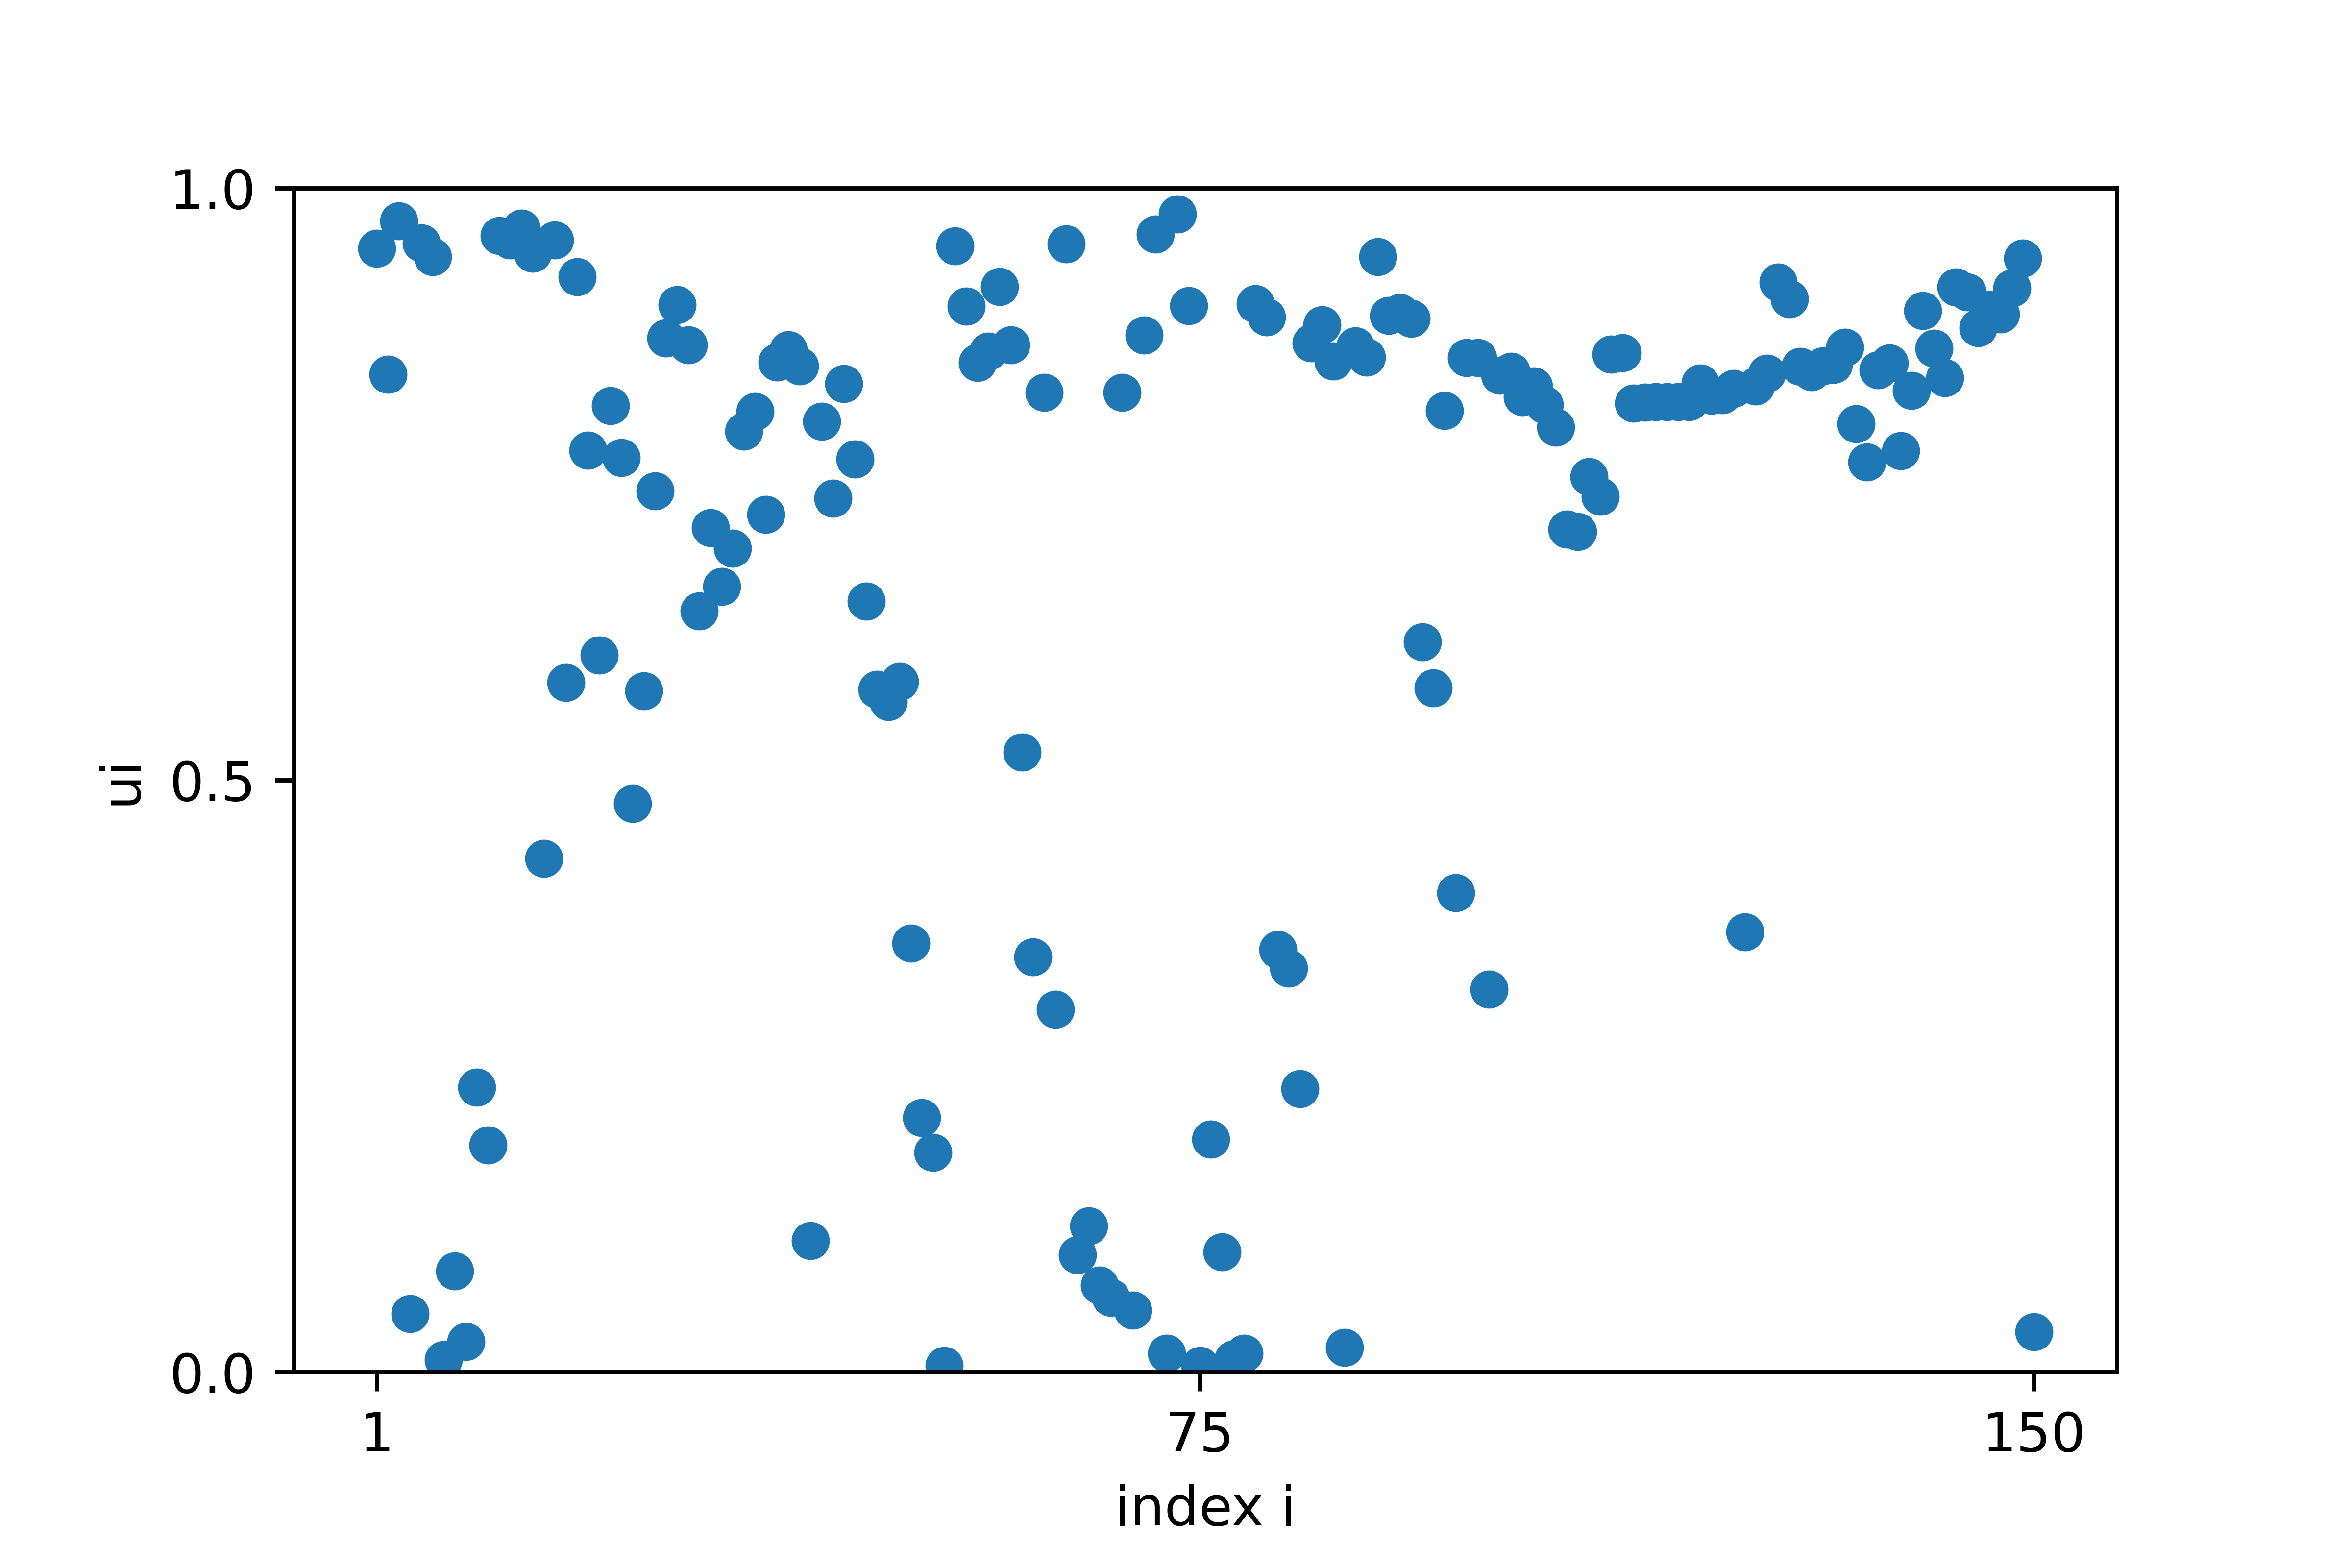
\includegraphics[width=1\linewidth]{u_lambda=0.93_t=2000.png}  
  \caption{$\lambda=0.93$}
\end{subfigure}
\hfill
\begin{subfigure}{.32\textwidth}
  \centering
  % include first image
  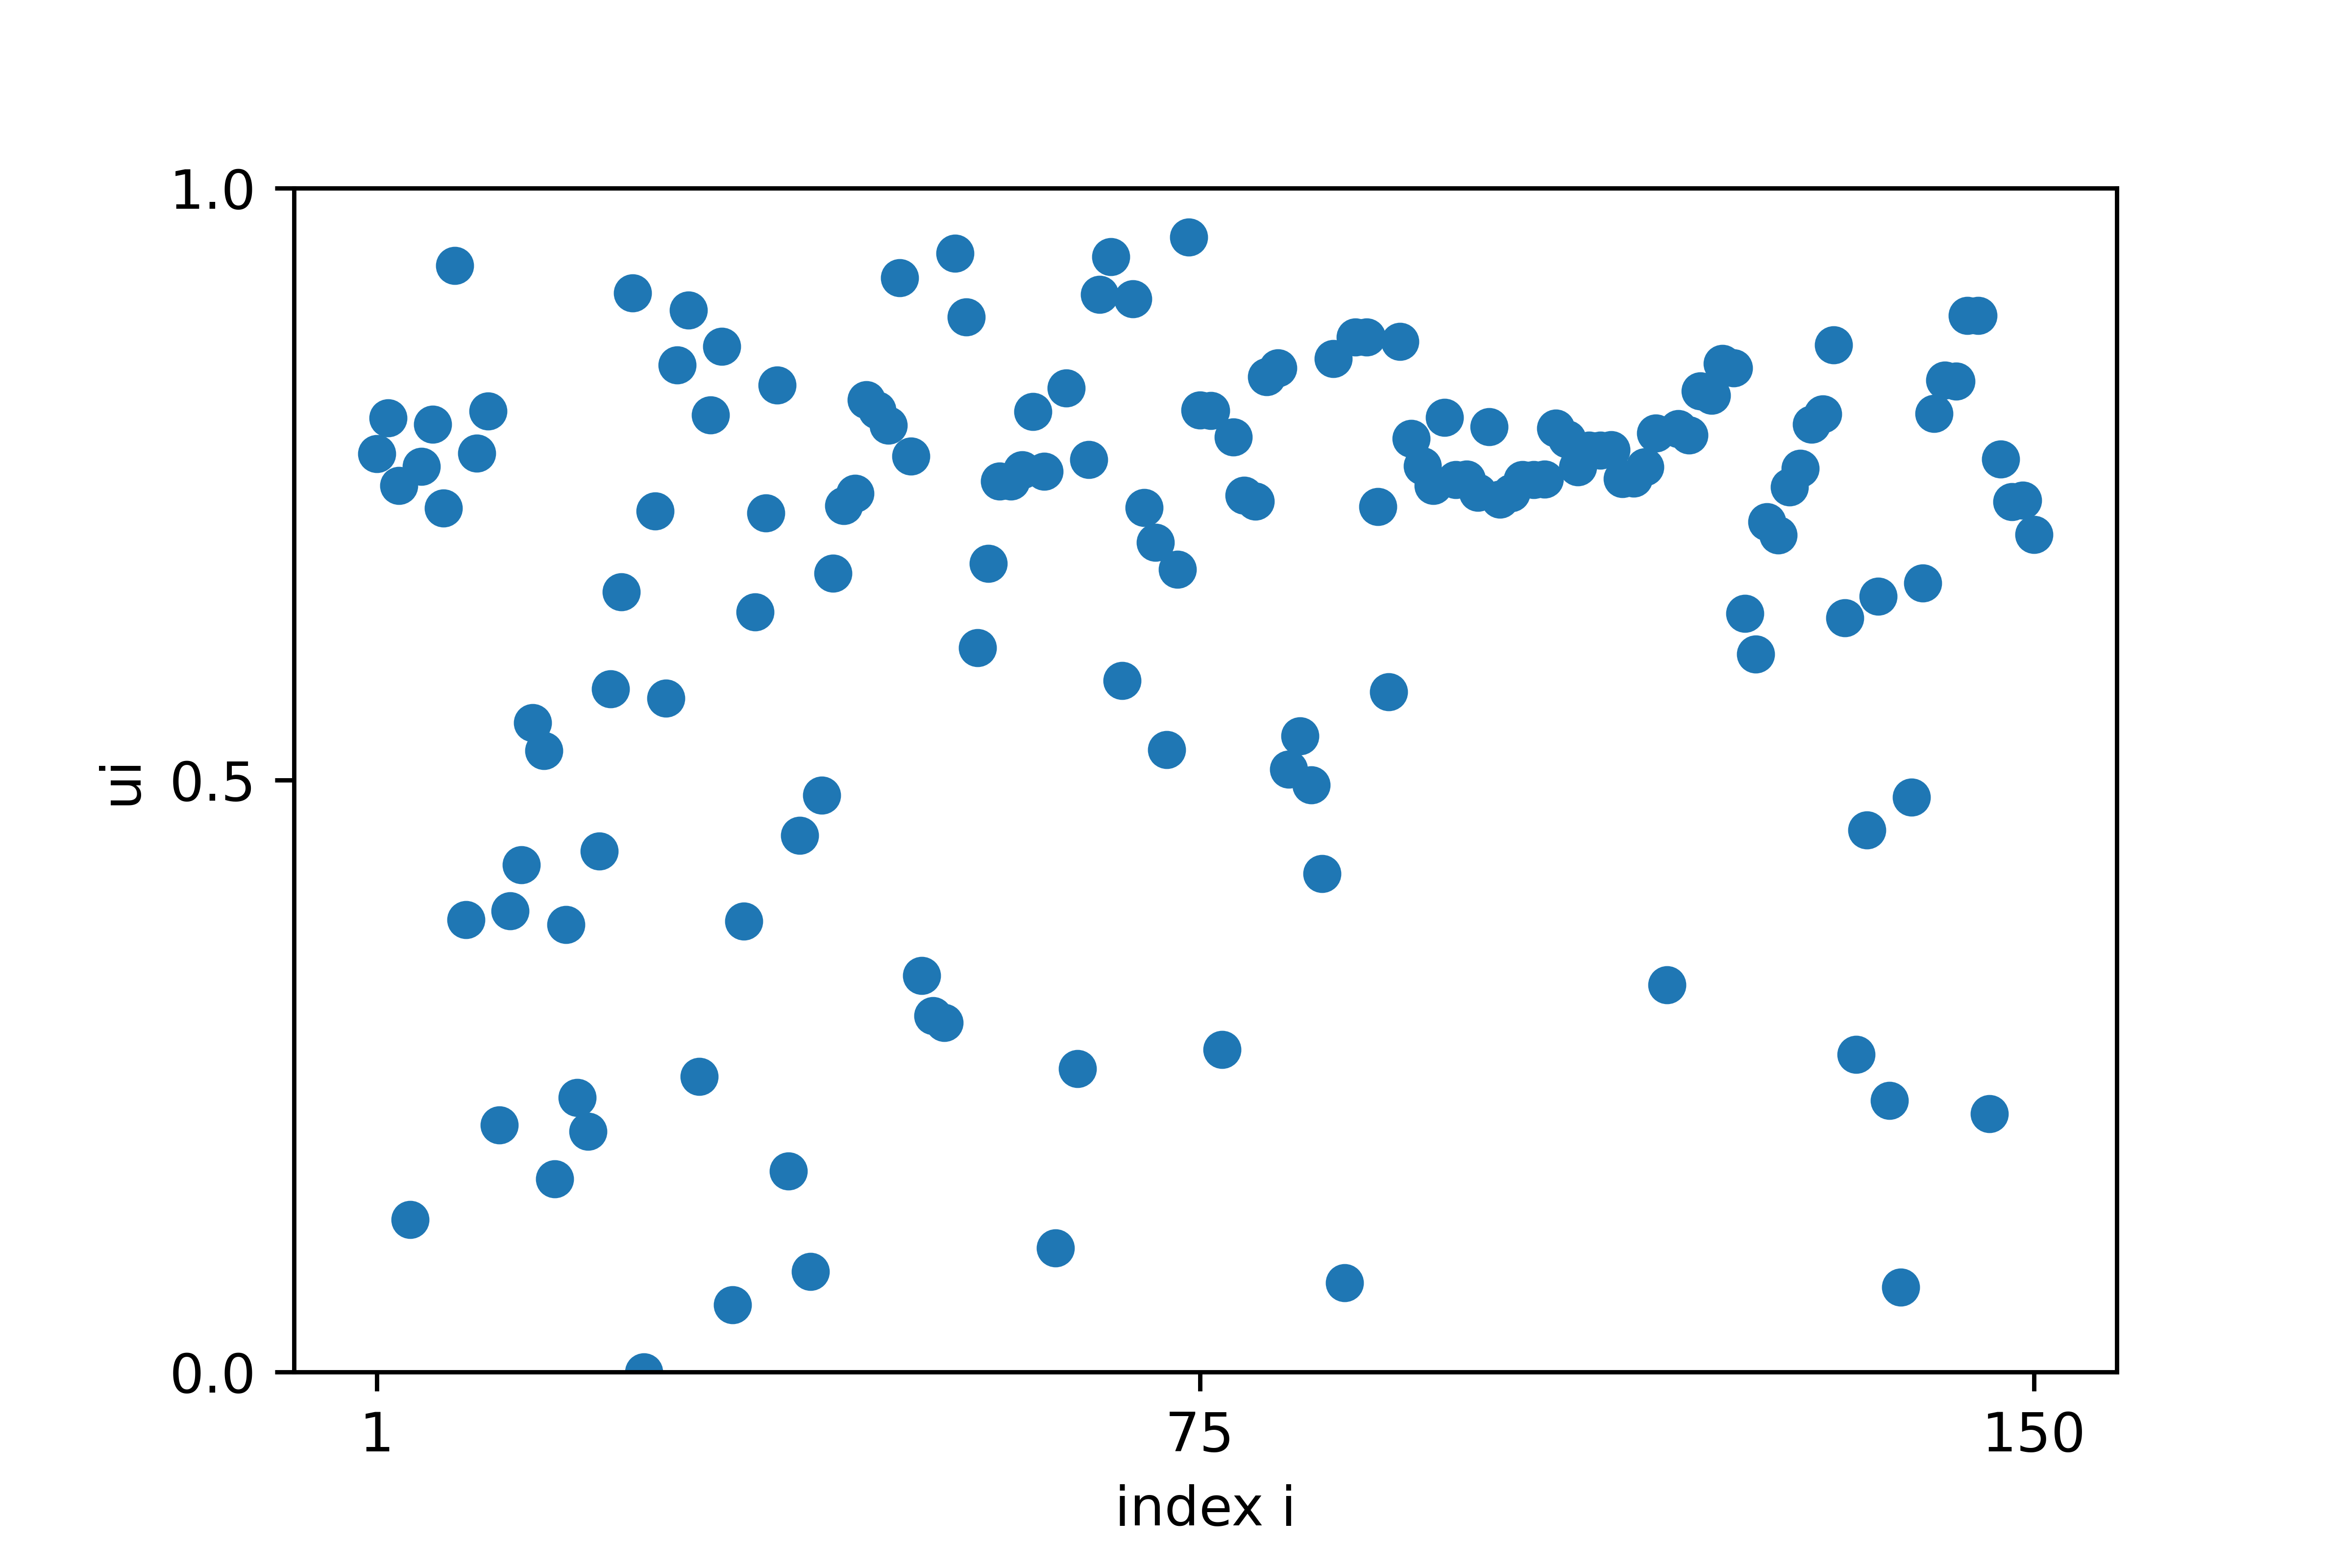
\includegraphics[width=1\linewidth]{u_lambda=0.92_t=2000}  
  \caption{$\lambda=0.92$}
\end{subfigure}
\begin{subfigure}{.32\textwidth}
  \centering
  % include first image
  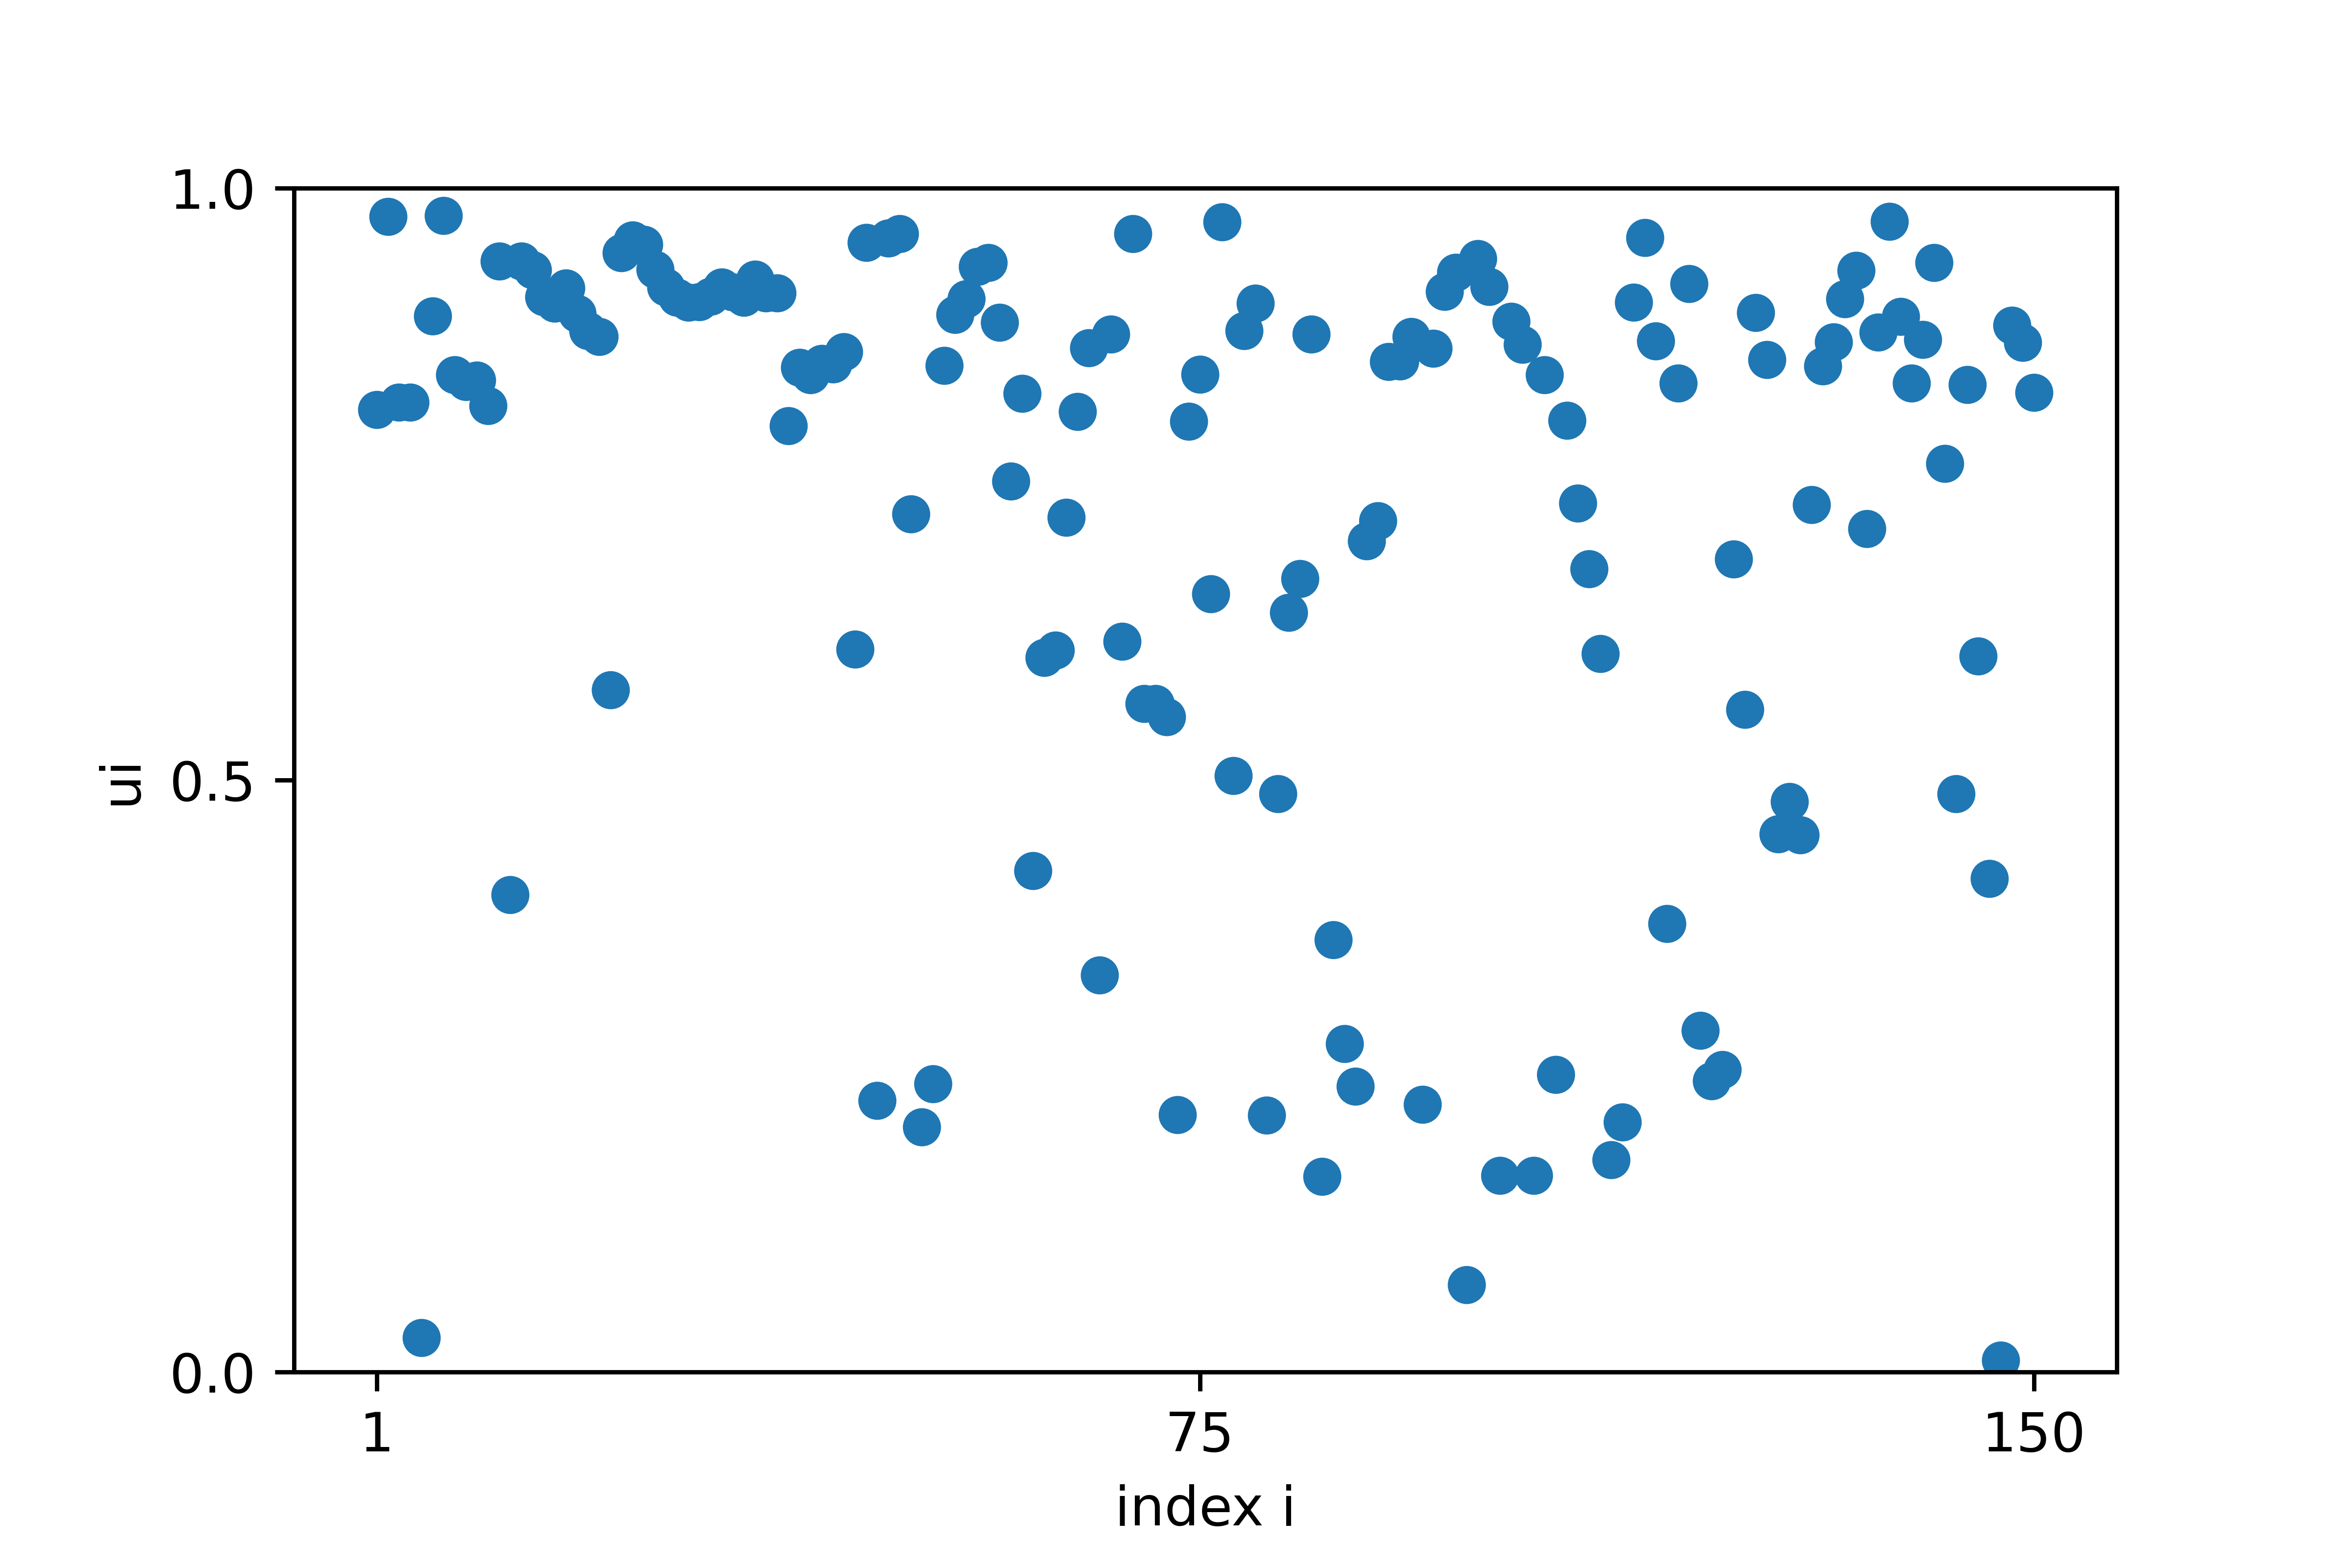
\includegraphics[width=1\linewidth]{u_lambda=0.91_t=2000.png}  
  \caption{$\lambda=0.91$}
\end{subfigure}
\hfill
\begin{subfigure}{.32\textwidth}
  \centering
  % include first image
  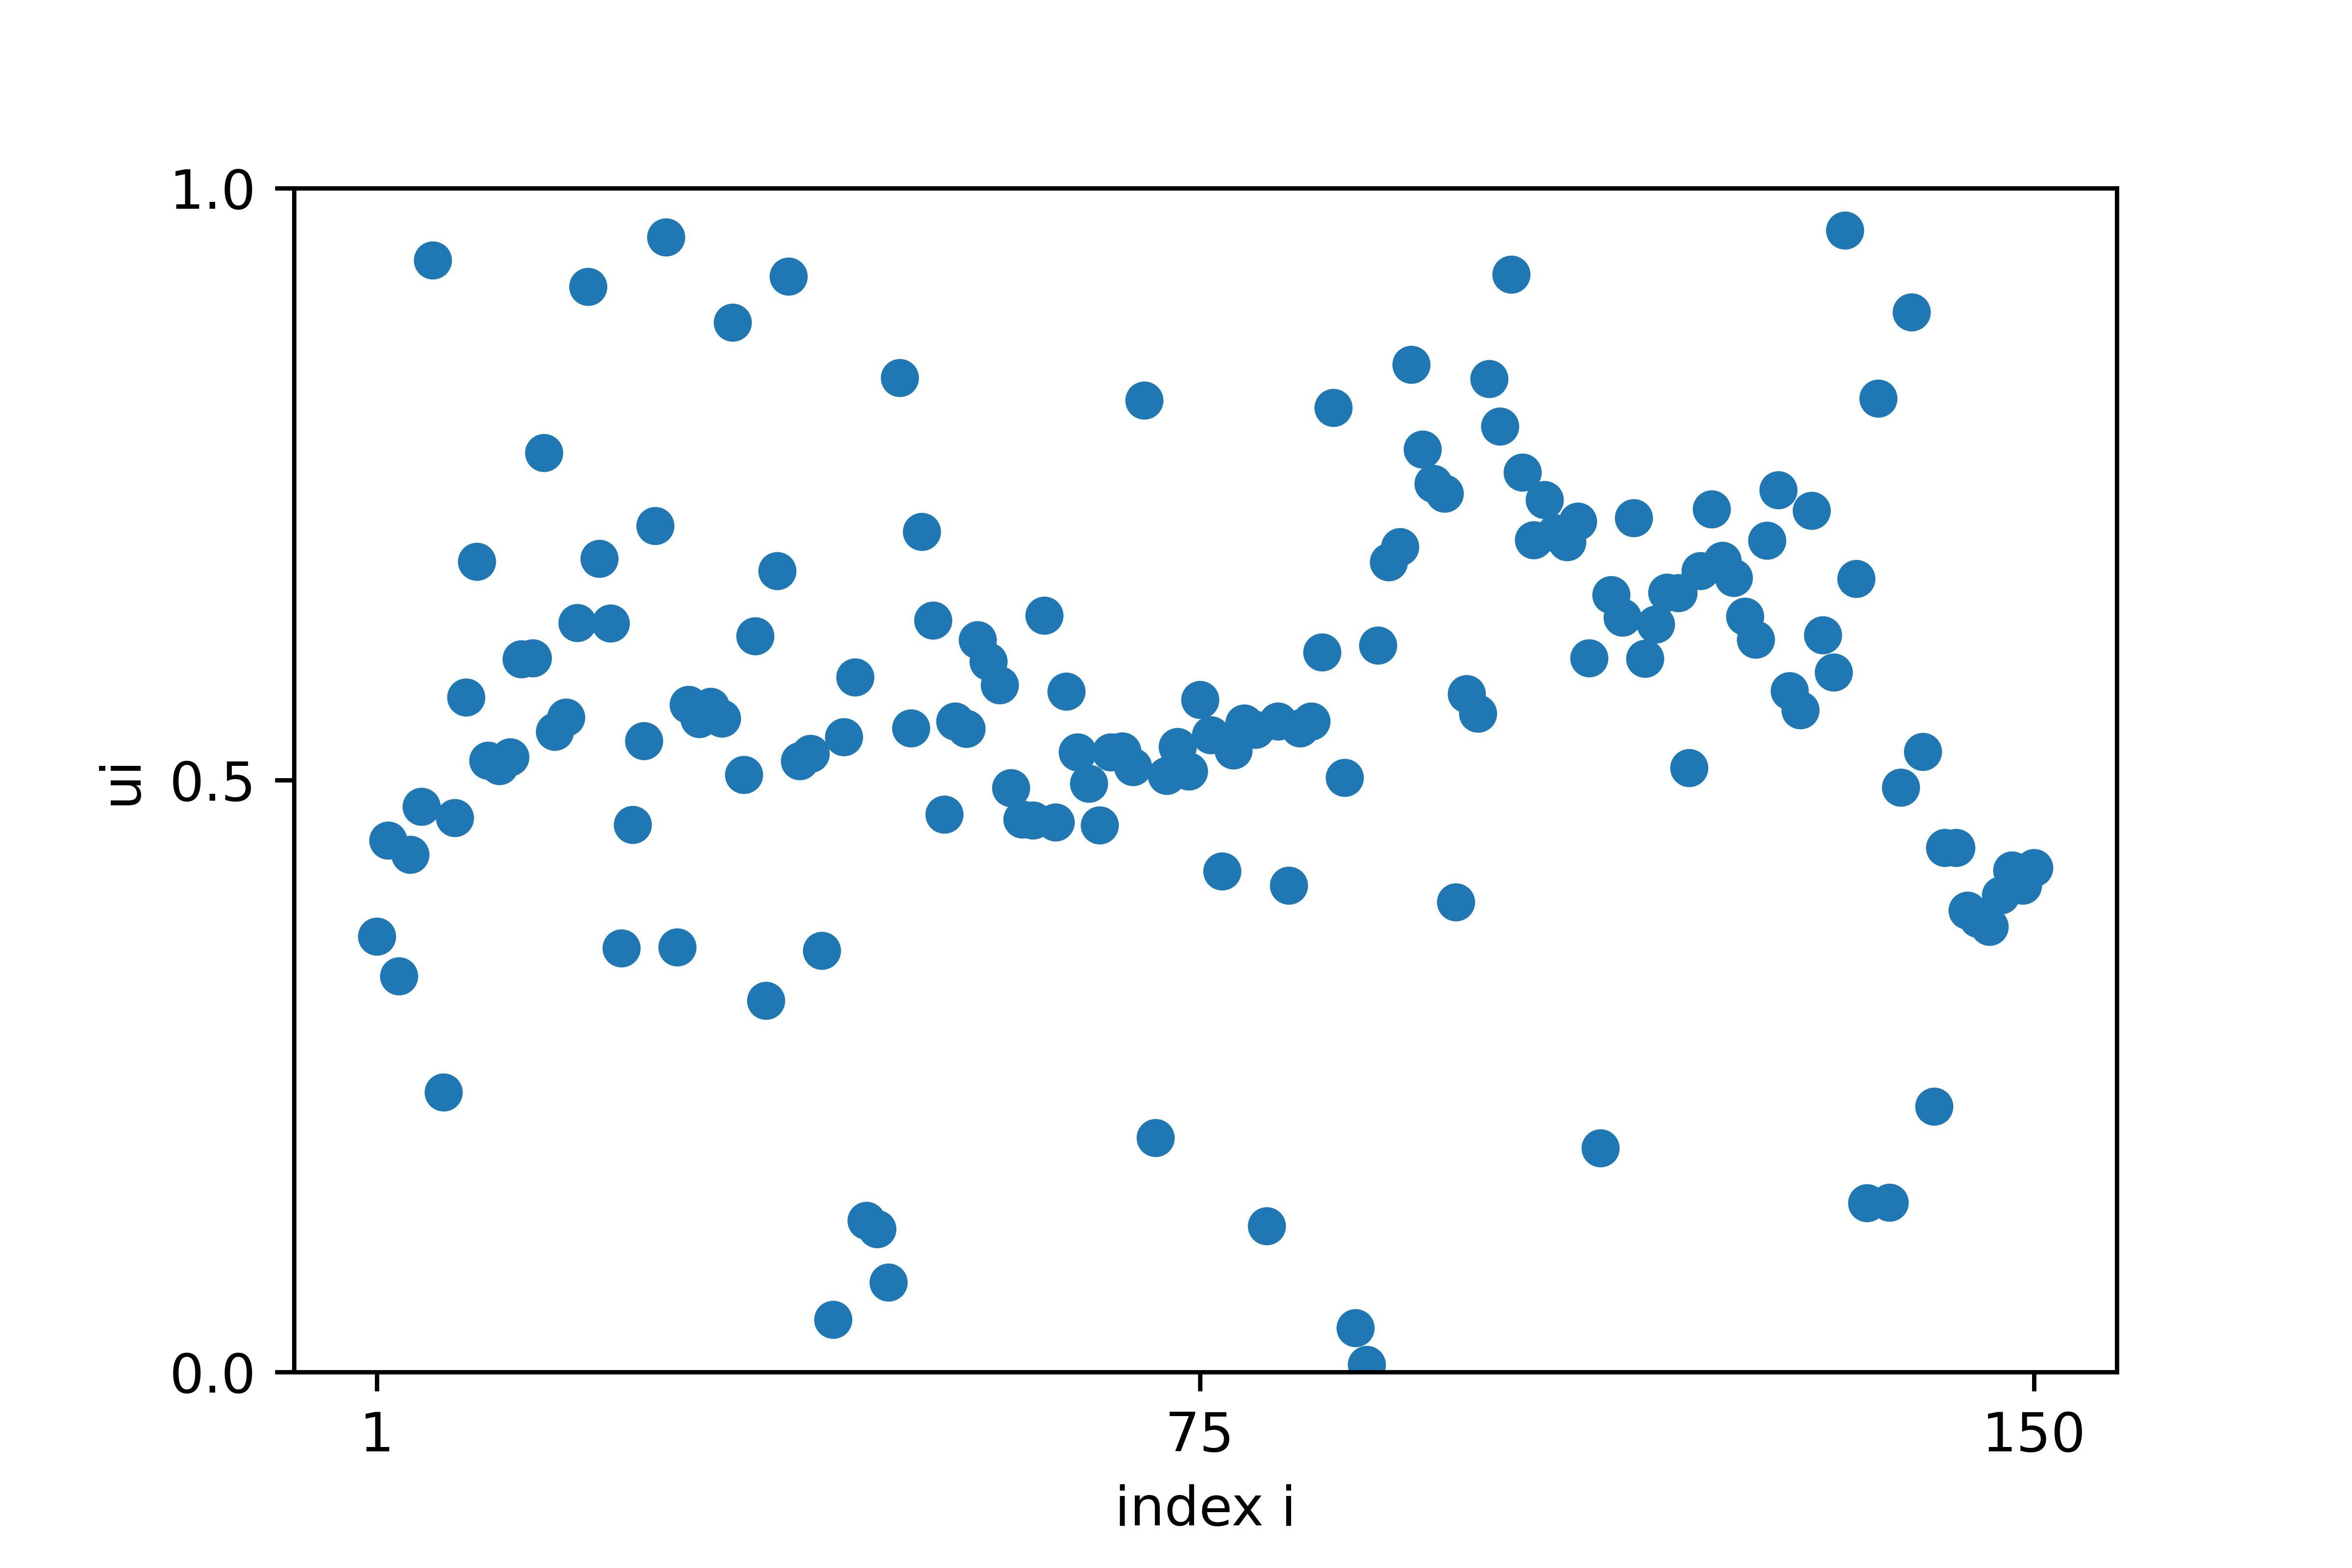
\includegraphics[width=1\linewidth]{u_lambda=0.9_t=2000.png}  
  \caption{$\lambda=0.90$}
\end{subfigure}
\hfill
\begin{subfigure}{.32\textwidth}
  \centering
  % include first image
  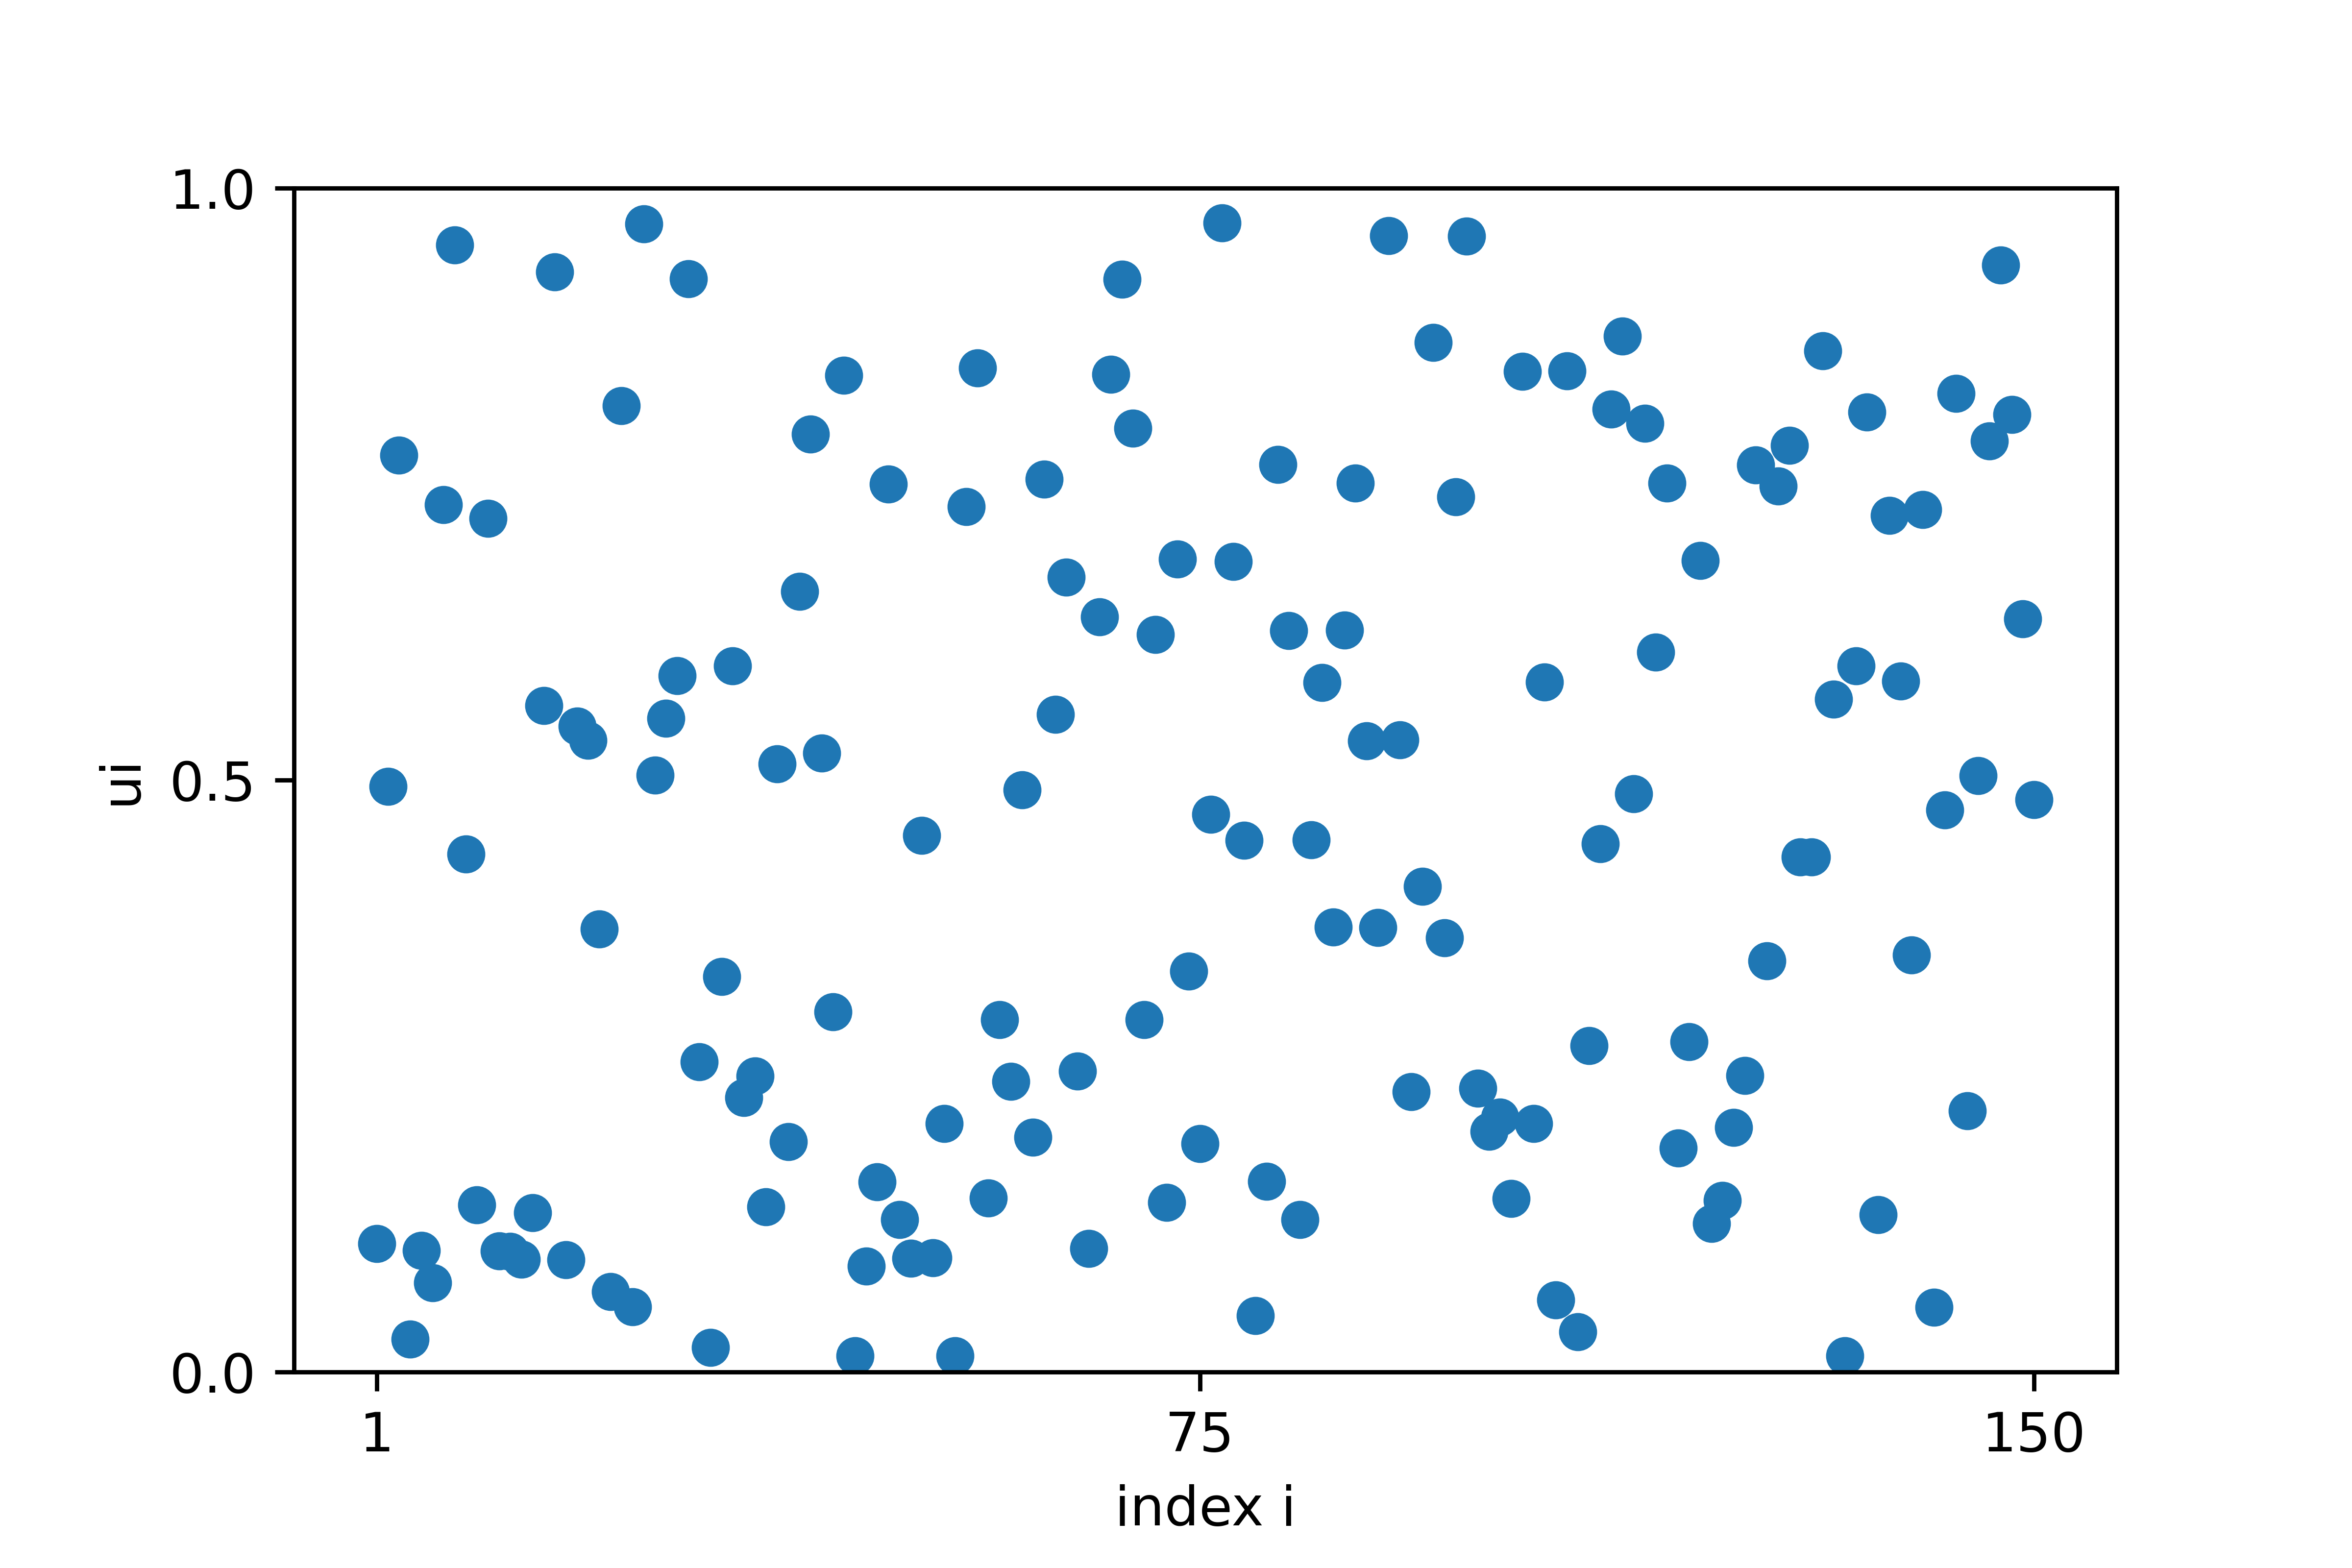
\includegraphics[width=1\linewidth]{u_lambda=0.8_t=2000.png}  
  \caption{$\lambda=0.80$}
\end{subfigure}

\caption{Snapshots of the membrane potential $u_i$ at $t=2000$ time units, for $N=150$, $r=0.4$ and $\sigma = 0.7$ and for various values of $\lambda$.}
\label{uivslmd}
\end{figure}

\begin{figure}[H]
\begin{subfigure}{.32\textwidth}
  \centering
  % include first image
  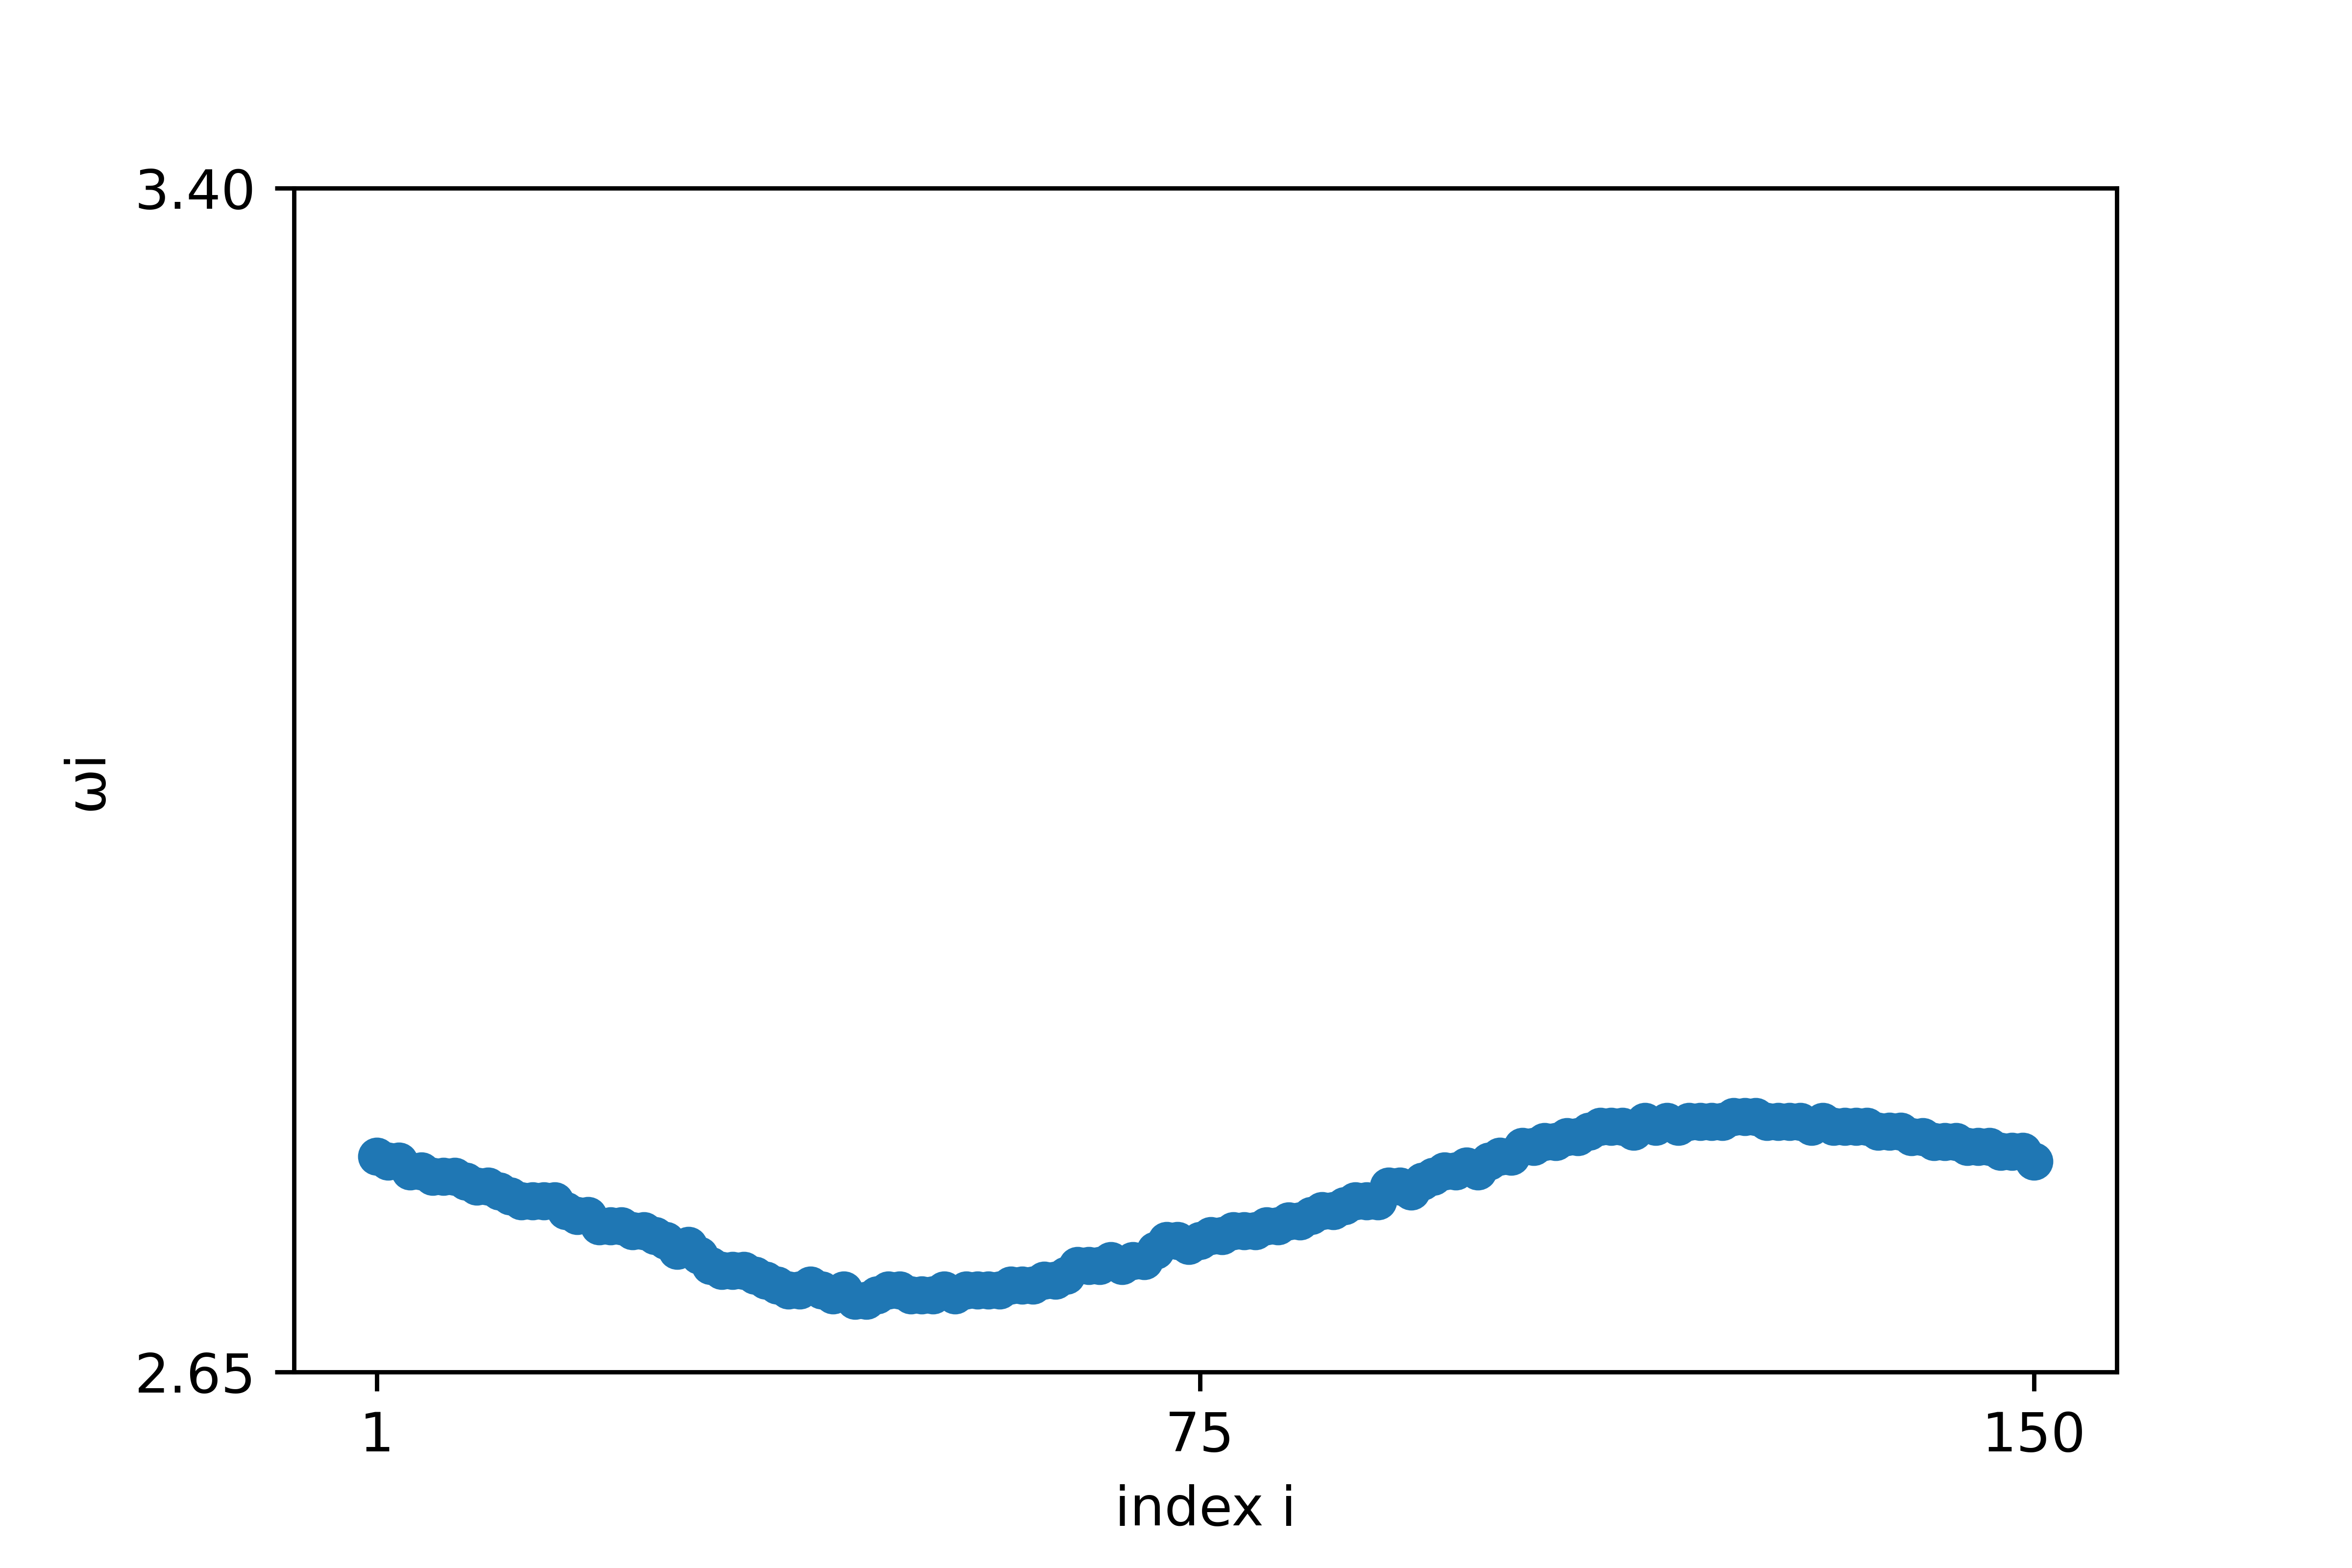
\includegraphics[width=1\linewidth]{w_lambda=1.0_t=2000.png}  
  \caption{$\lambda=1.00$}
\end{subfigure}
\hfill
\begin{subfigure}{.32\textwidth}
  \centering
  % include second image
  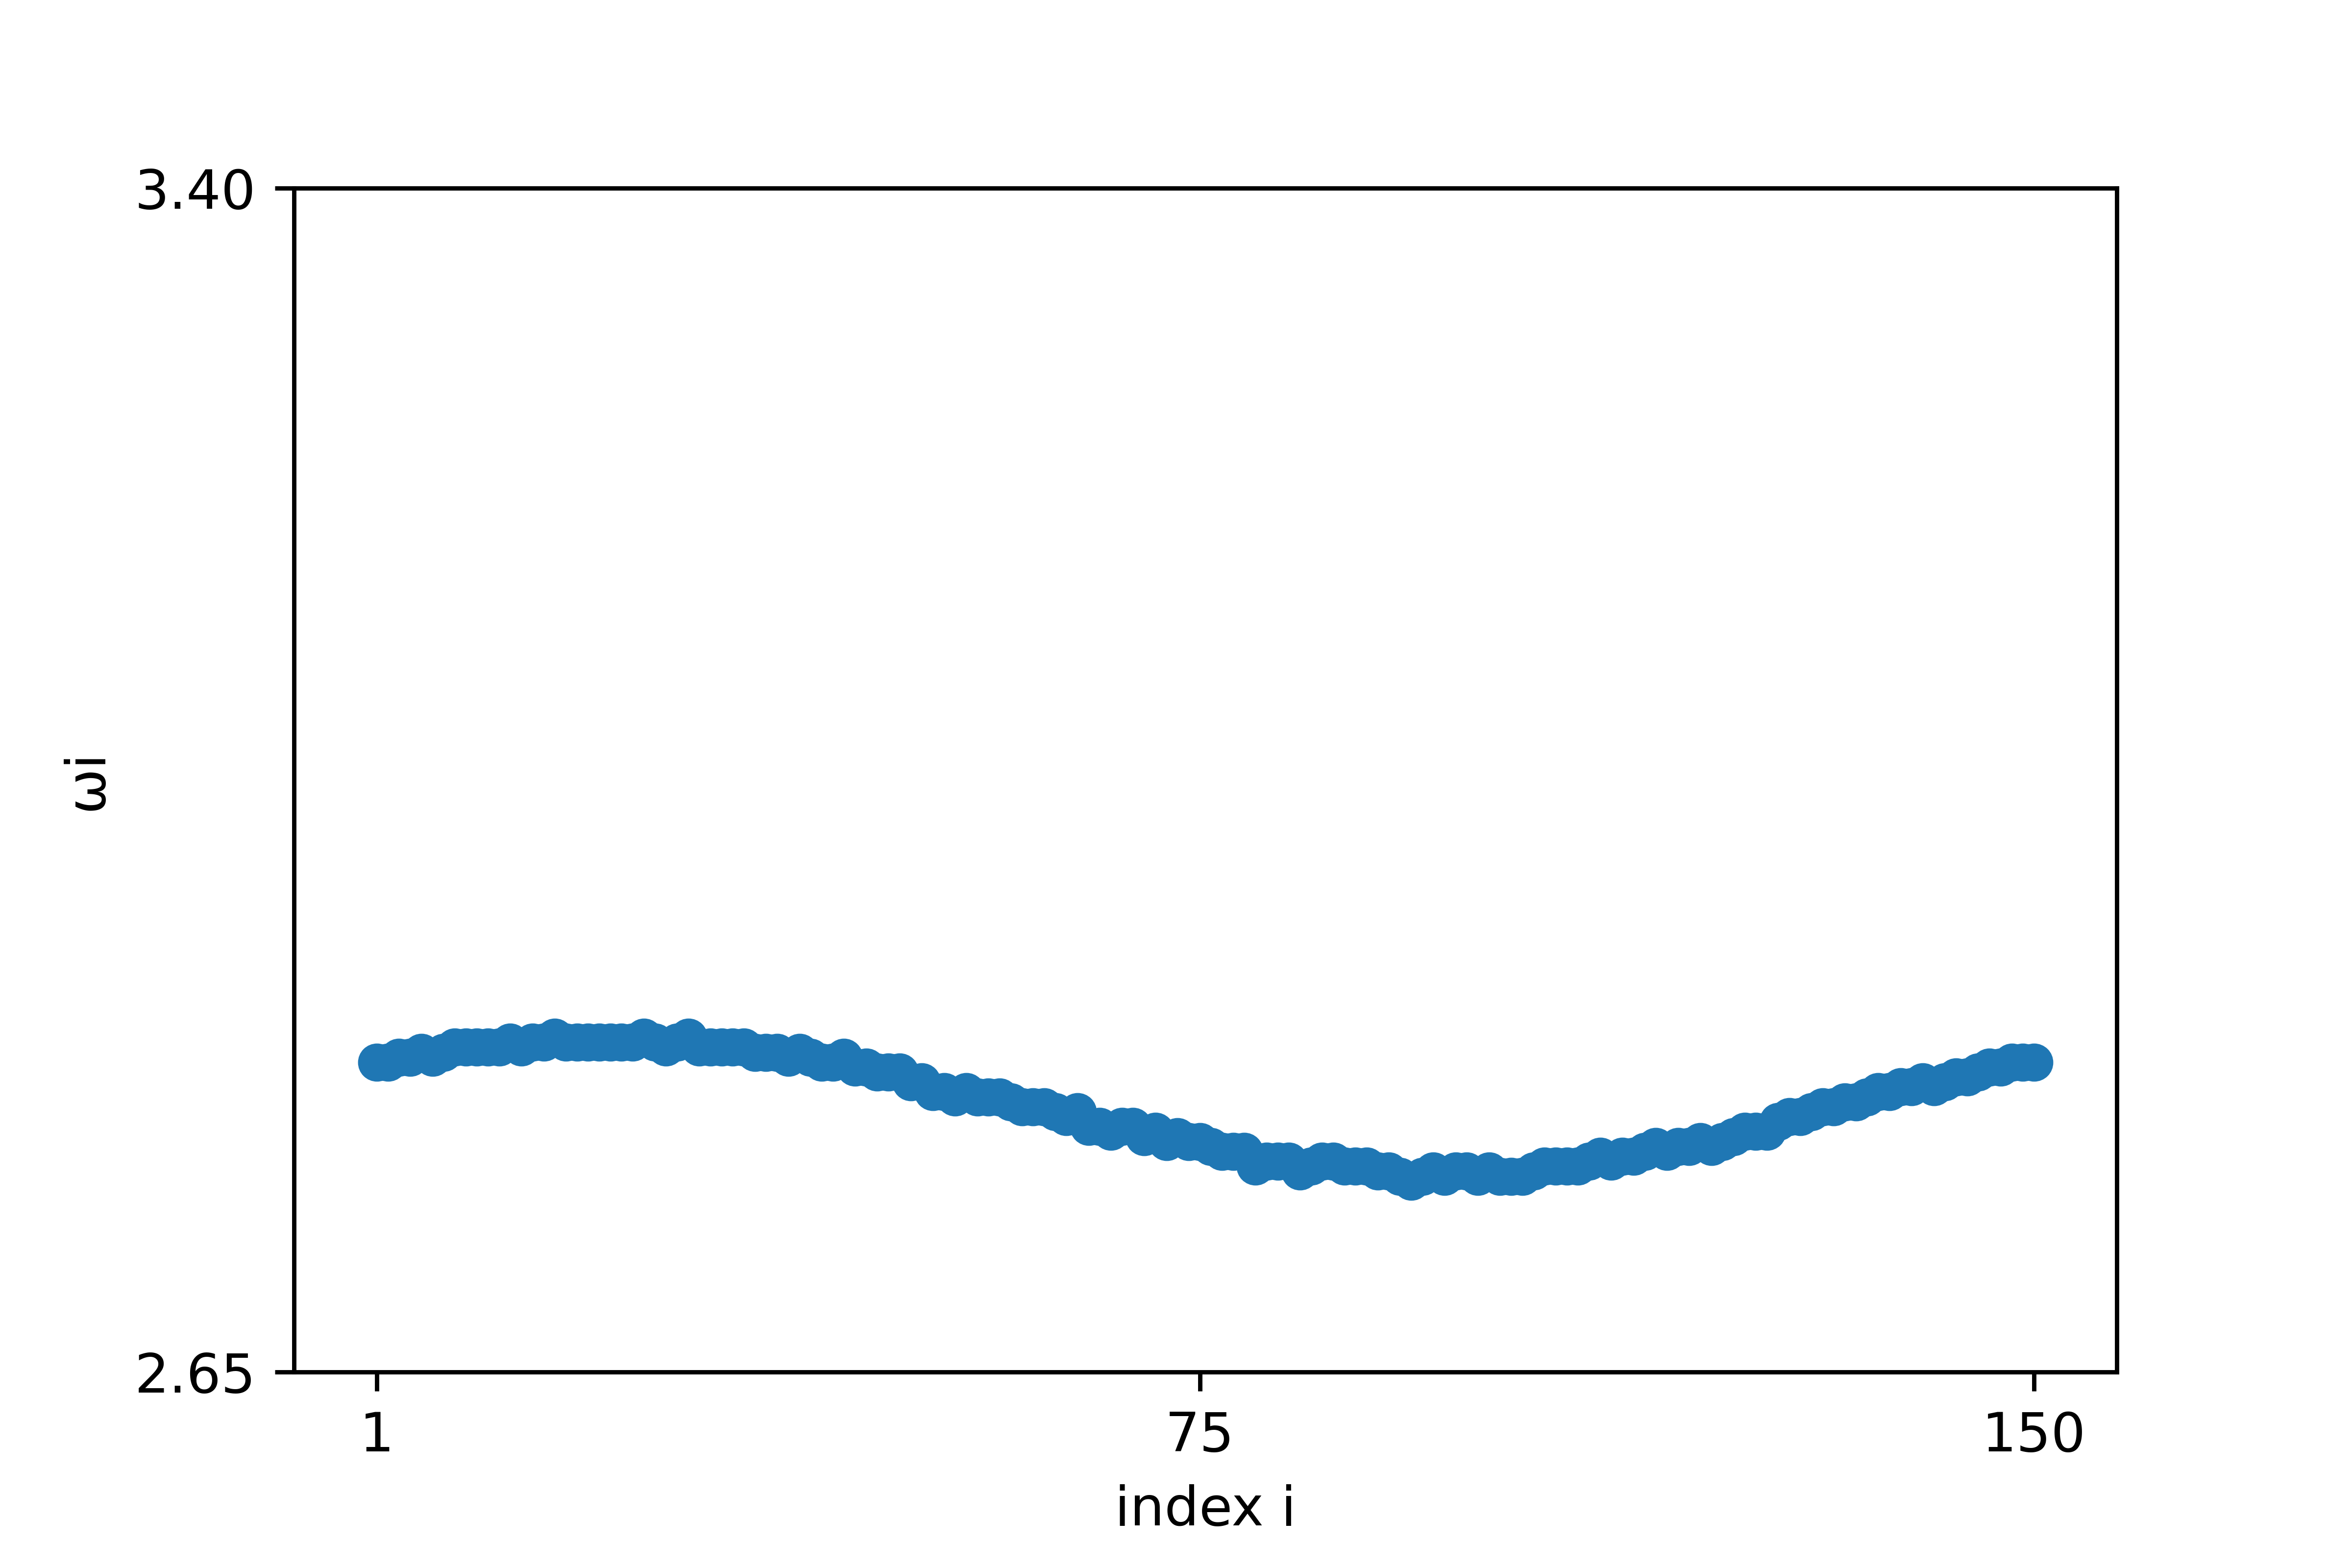
\includegraphics[width=1\linewidth]{w_lambda=0.99_t=2000.png}  
  \caption{$\lambda=0.99$}
\end{subfigure}
\hfill
\begin{subfigure}{.32\textwidth}
  \centering
  % include first image
  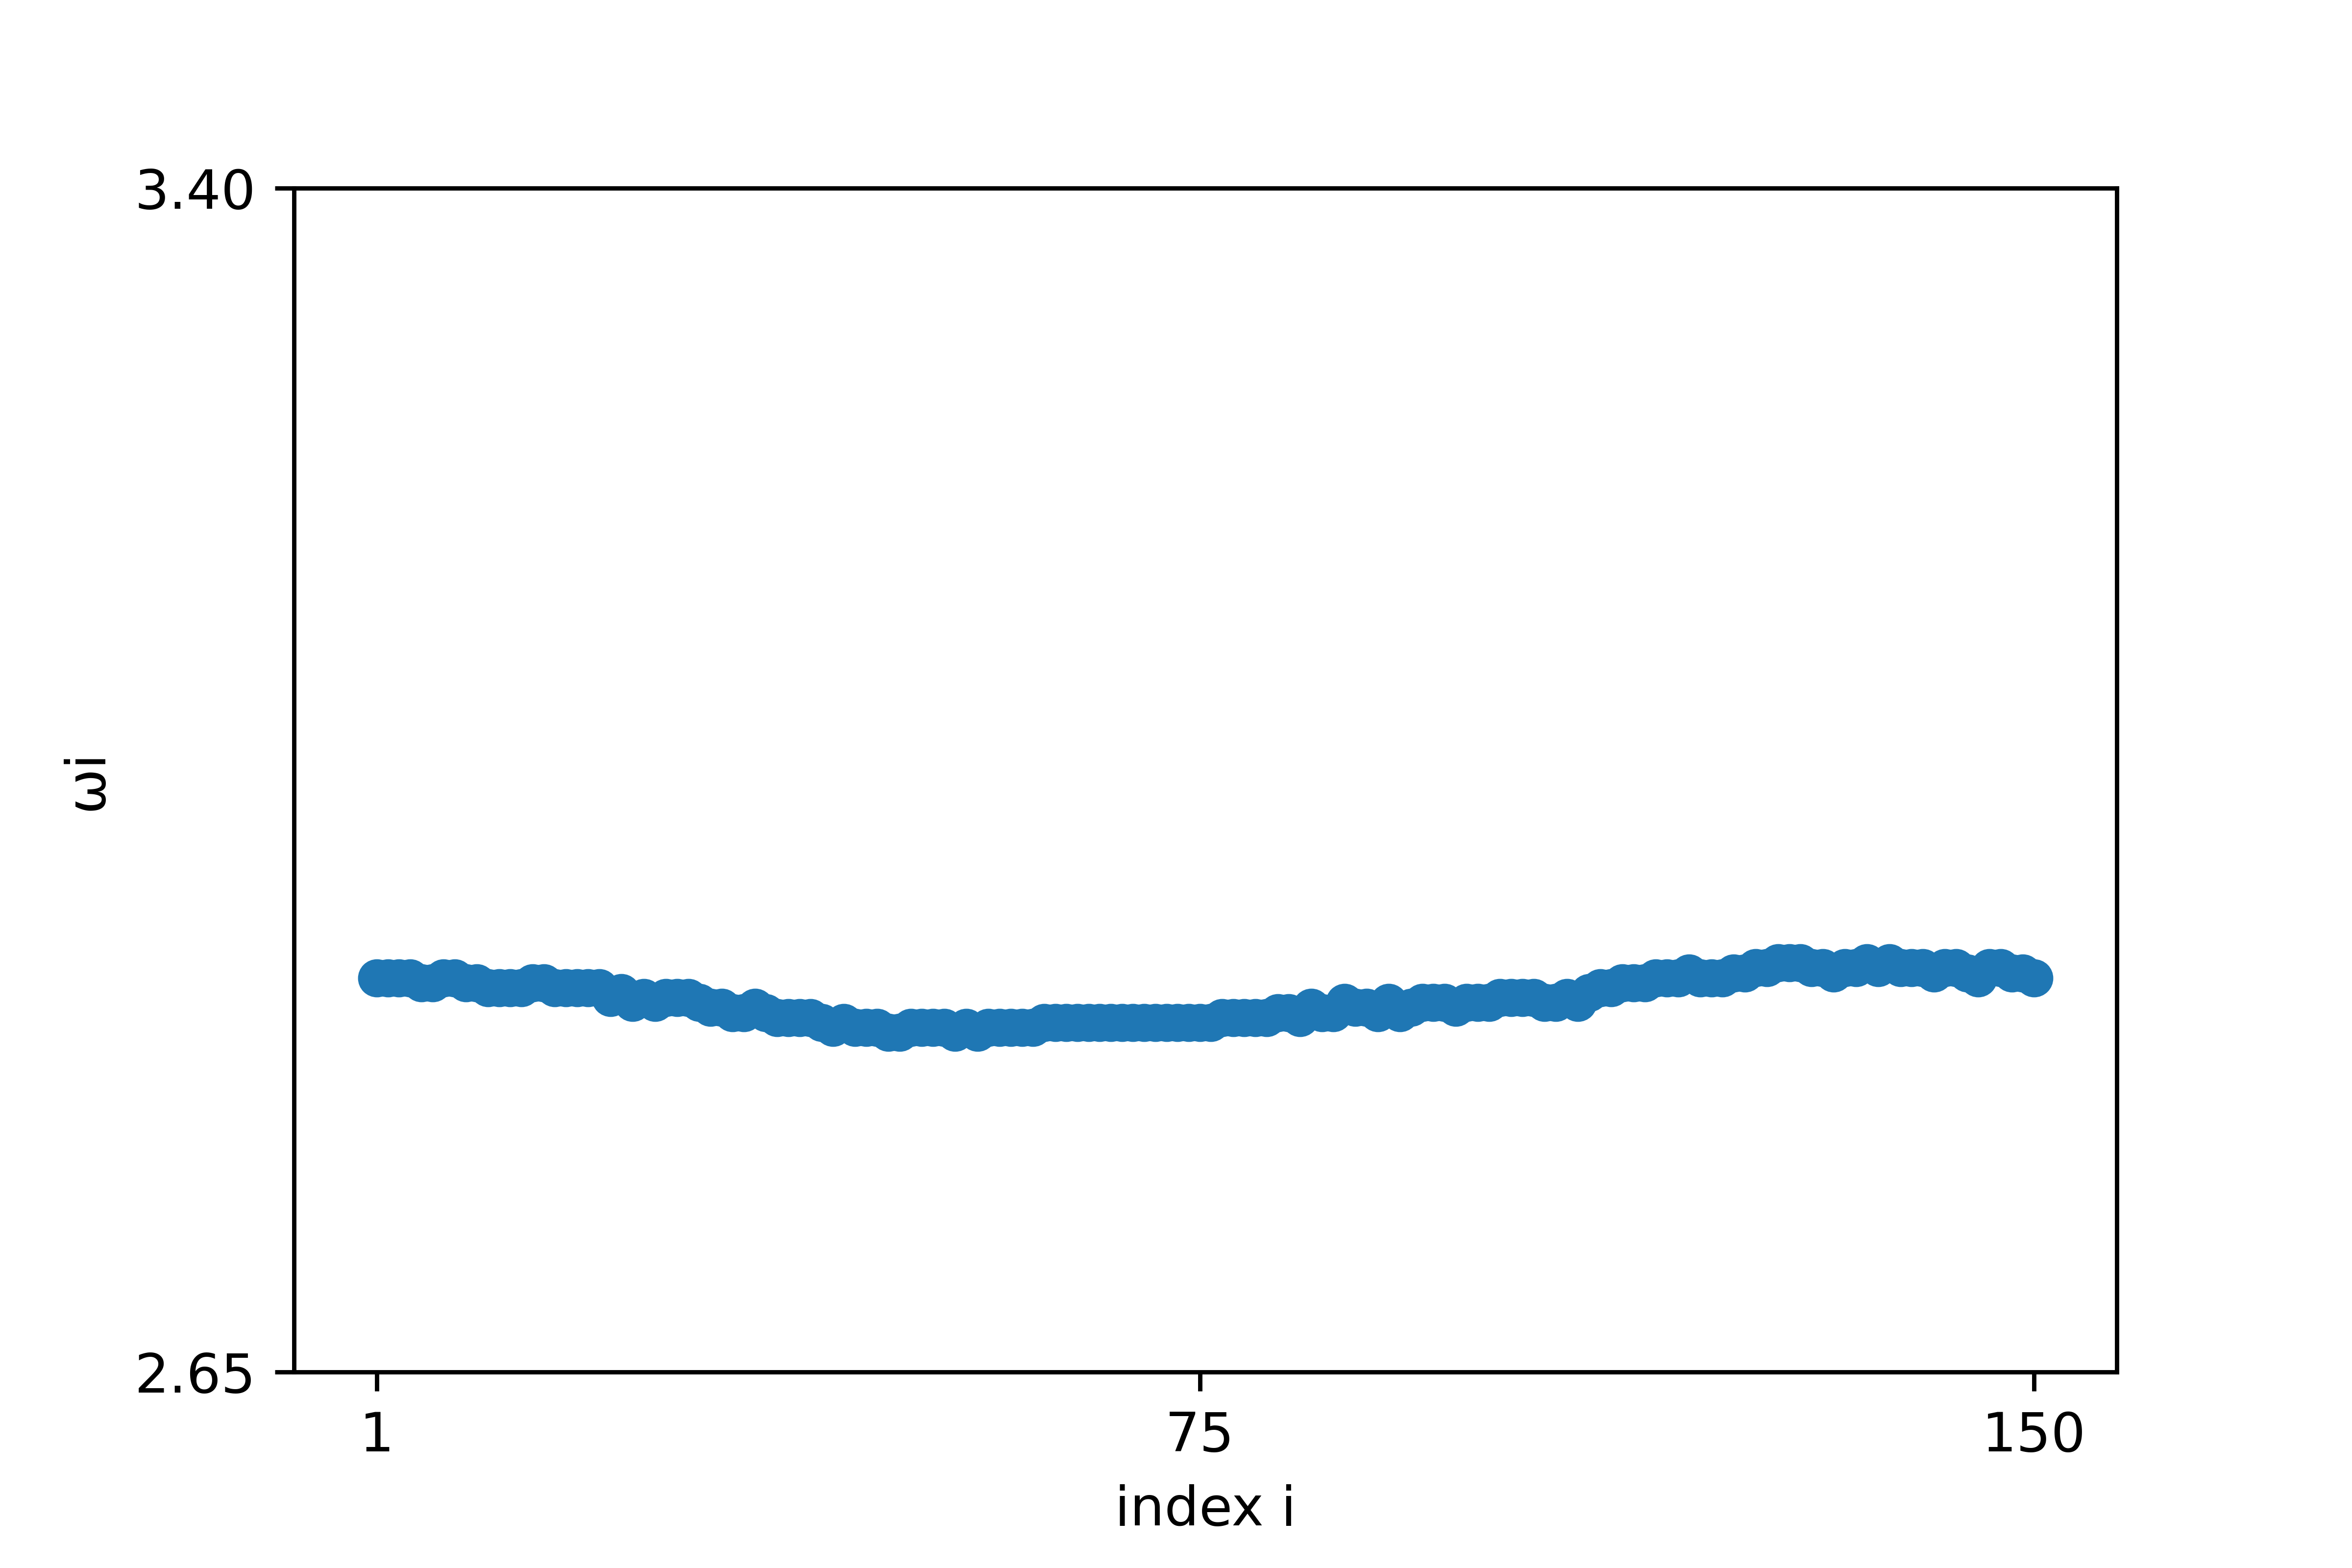
\includegraphics[width=1\linewidth]{w_lambda=0.98_t=2000}  
  \caption{$\lambda=0.98$}
\end{subfigure}
\begin{subfigure}{.32\textwidth}
  \centering
  % include first image
  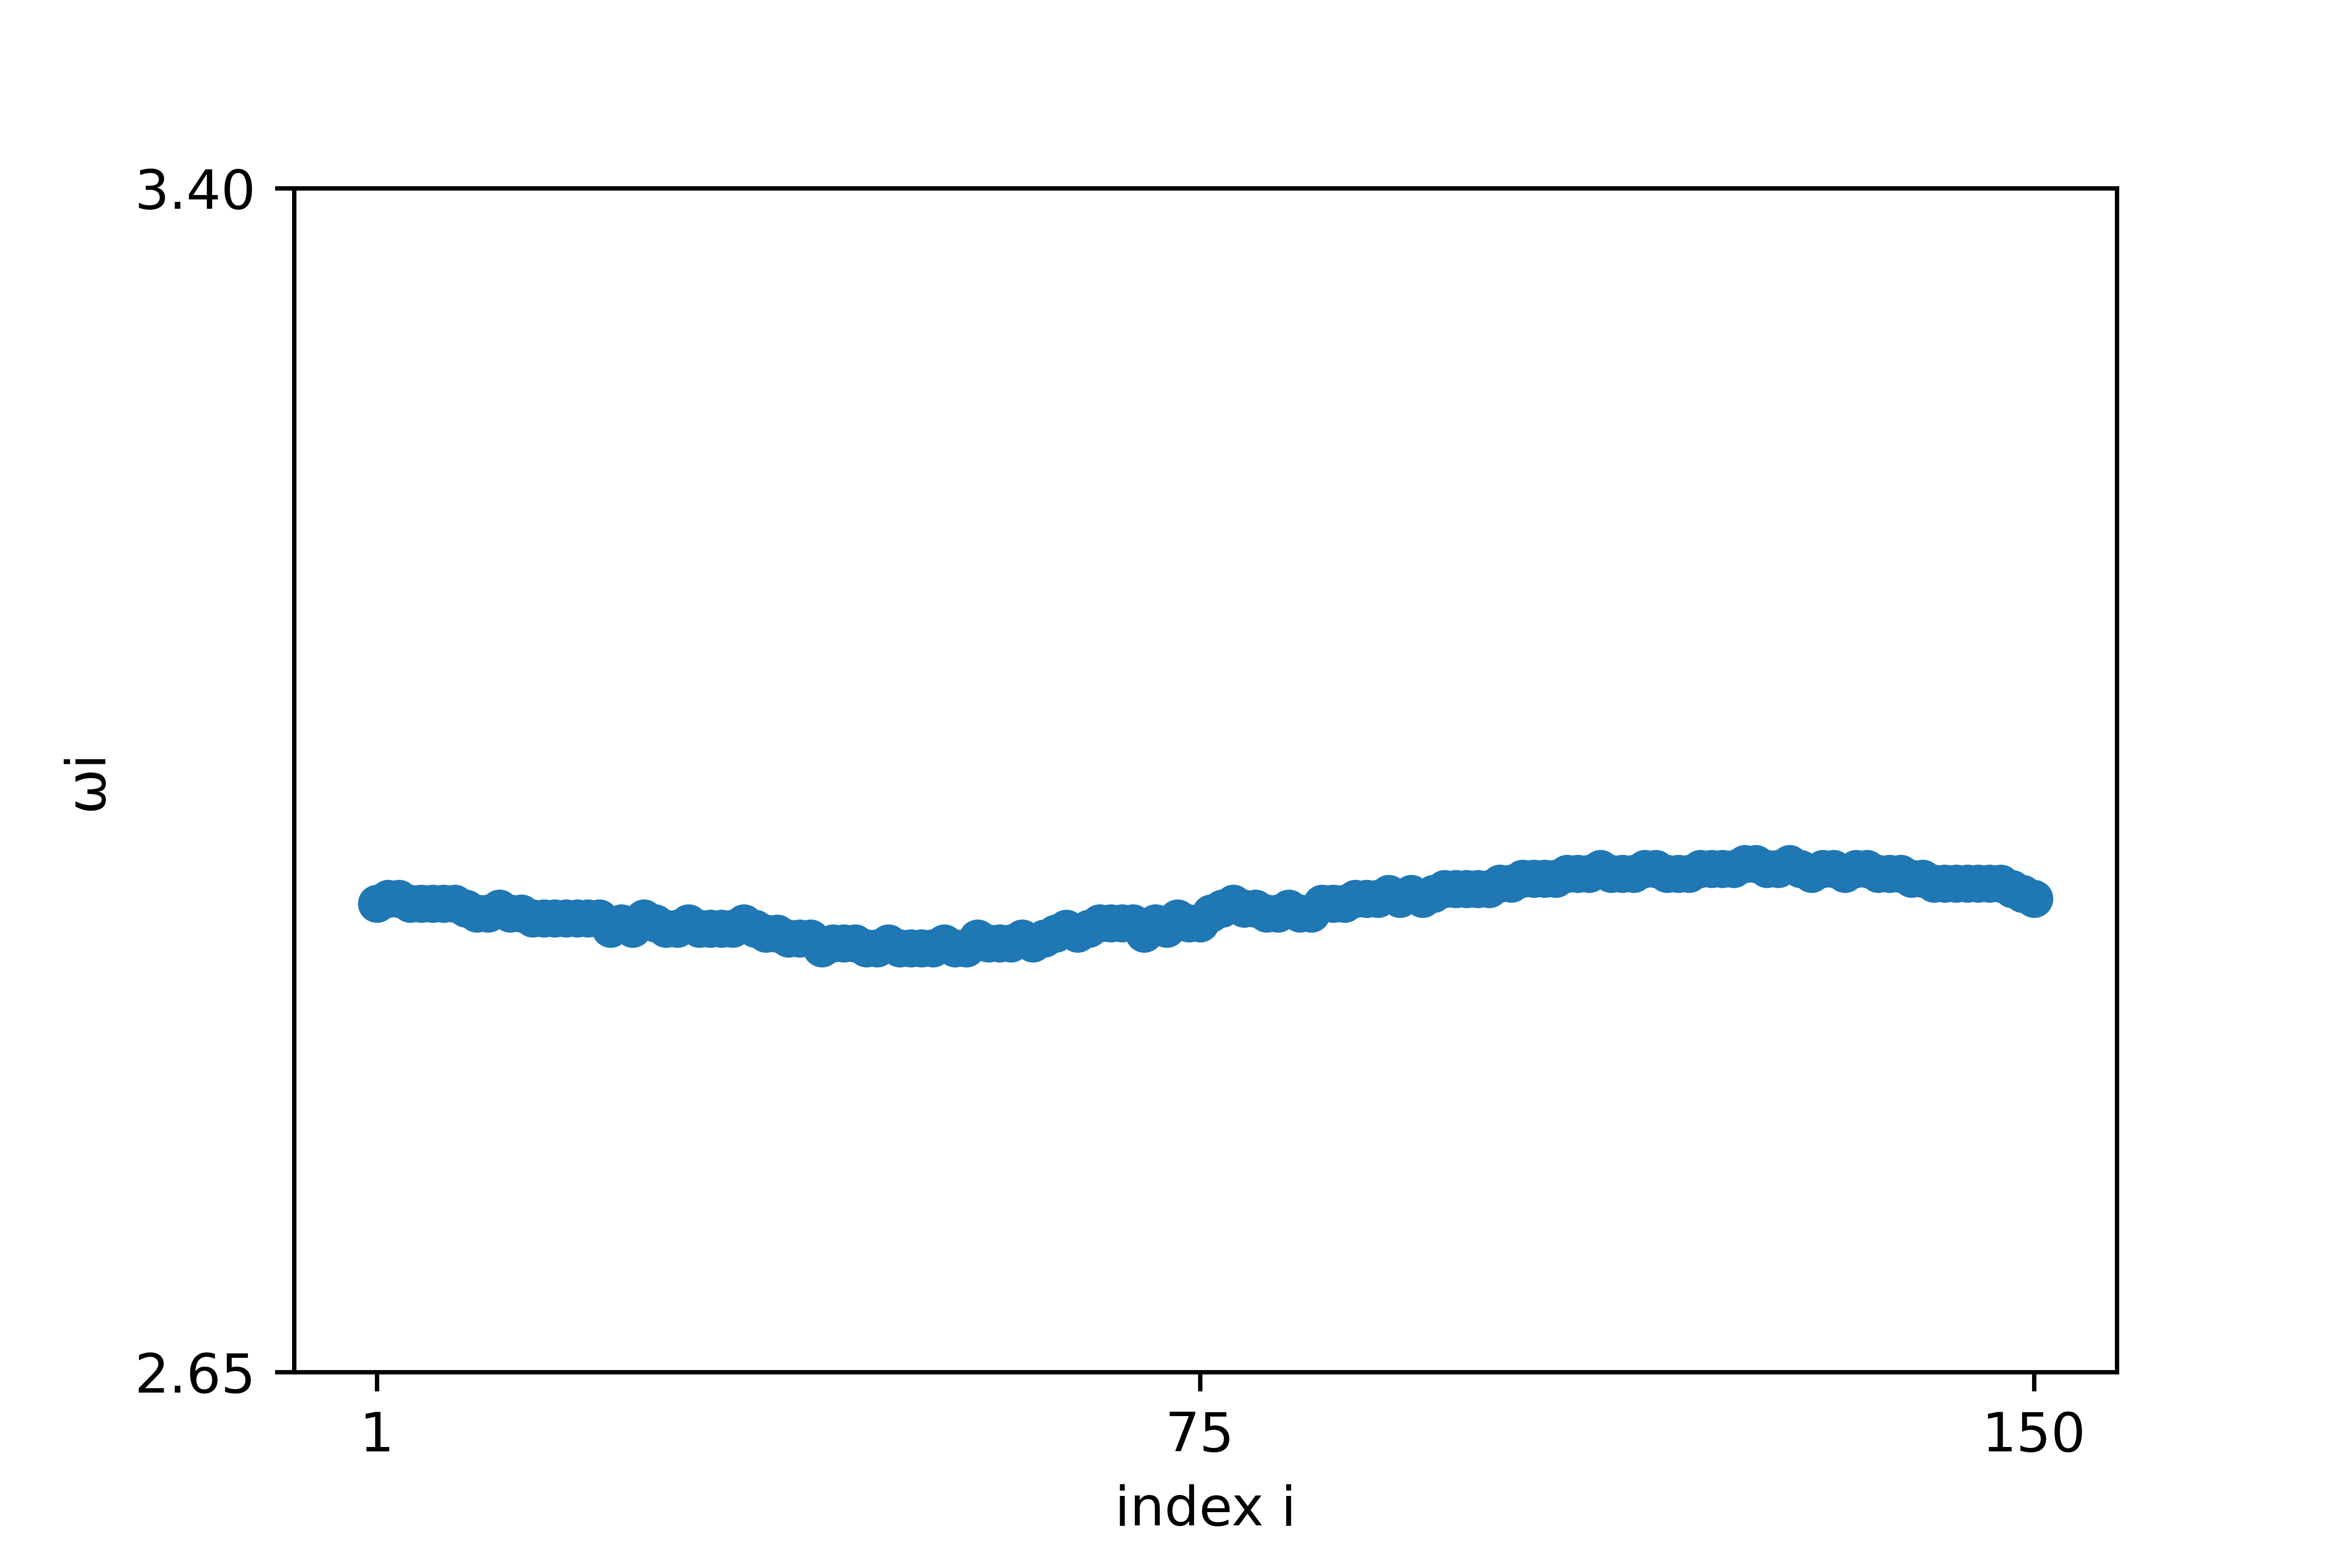
\includegraphics[width=1\linewidth]{w_lambda=0.97_t=2000.png}  
  \caption{$\lambda=0.97$}
\end{subfigure}
\hfill
\begin{subfigure}{.32\textwidth}
  \centering
  % include first image
  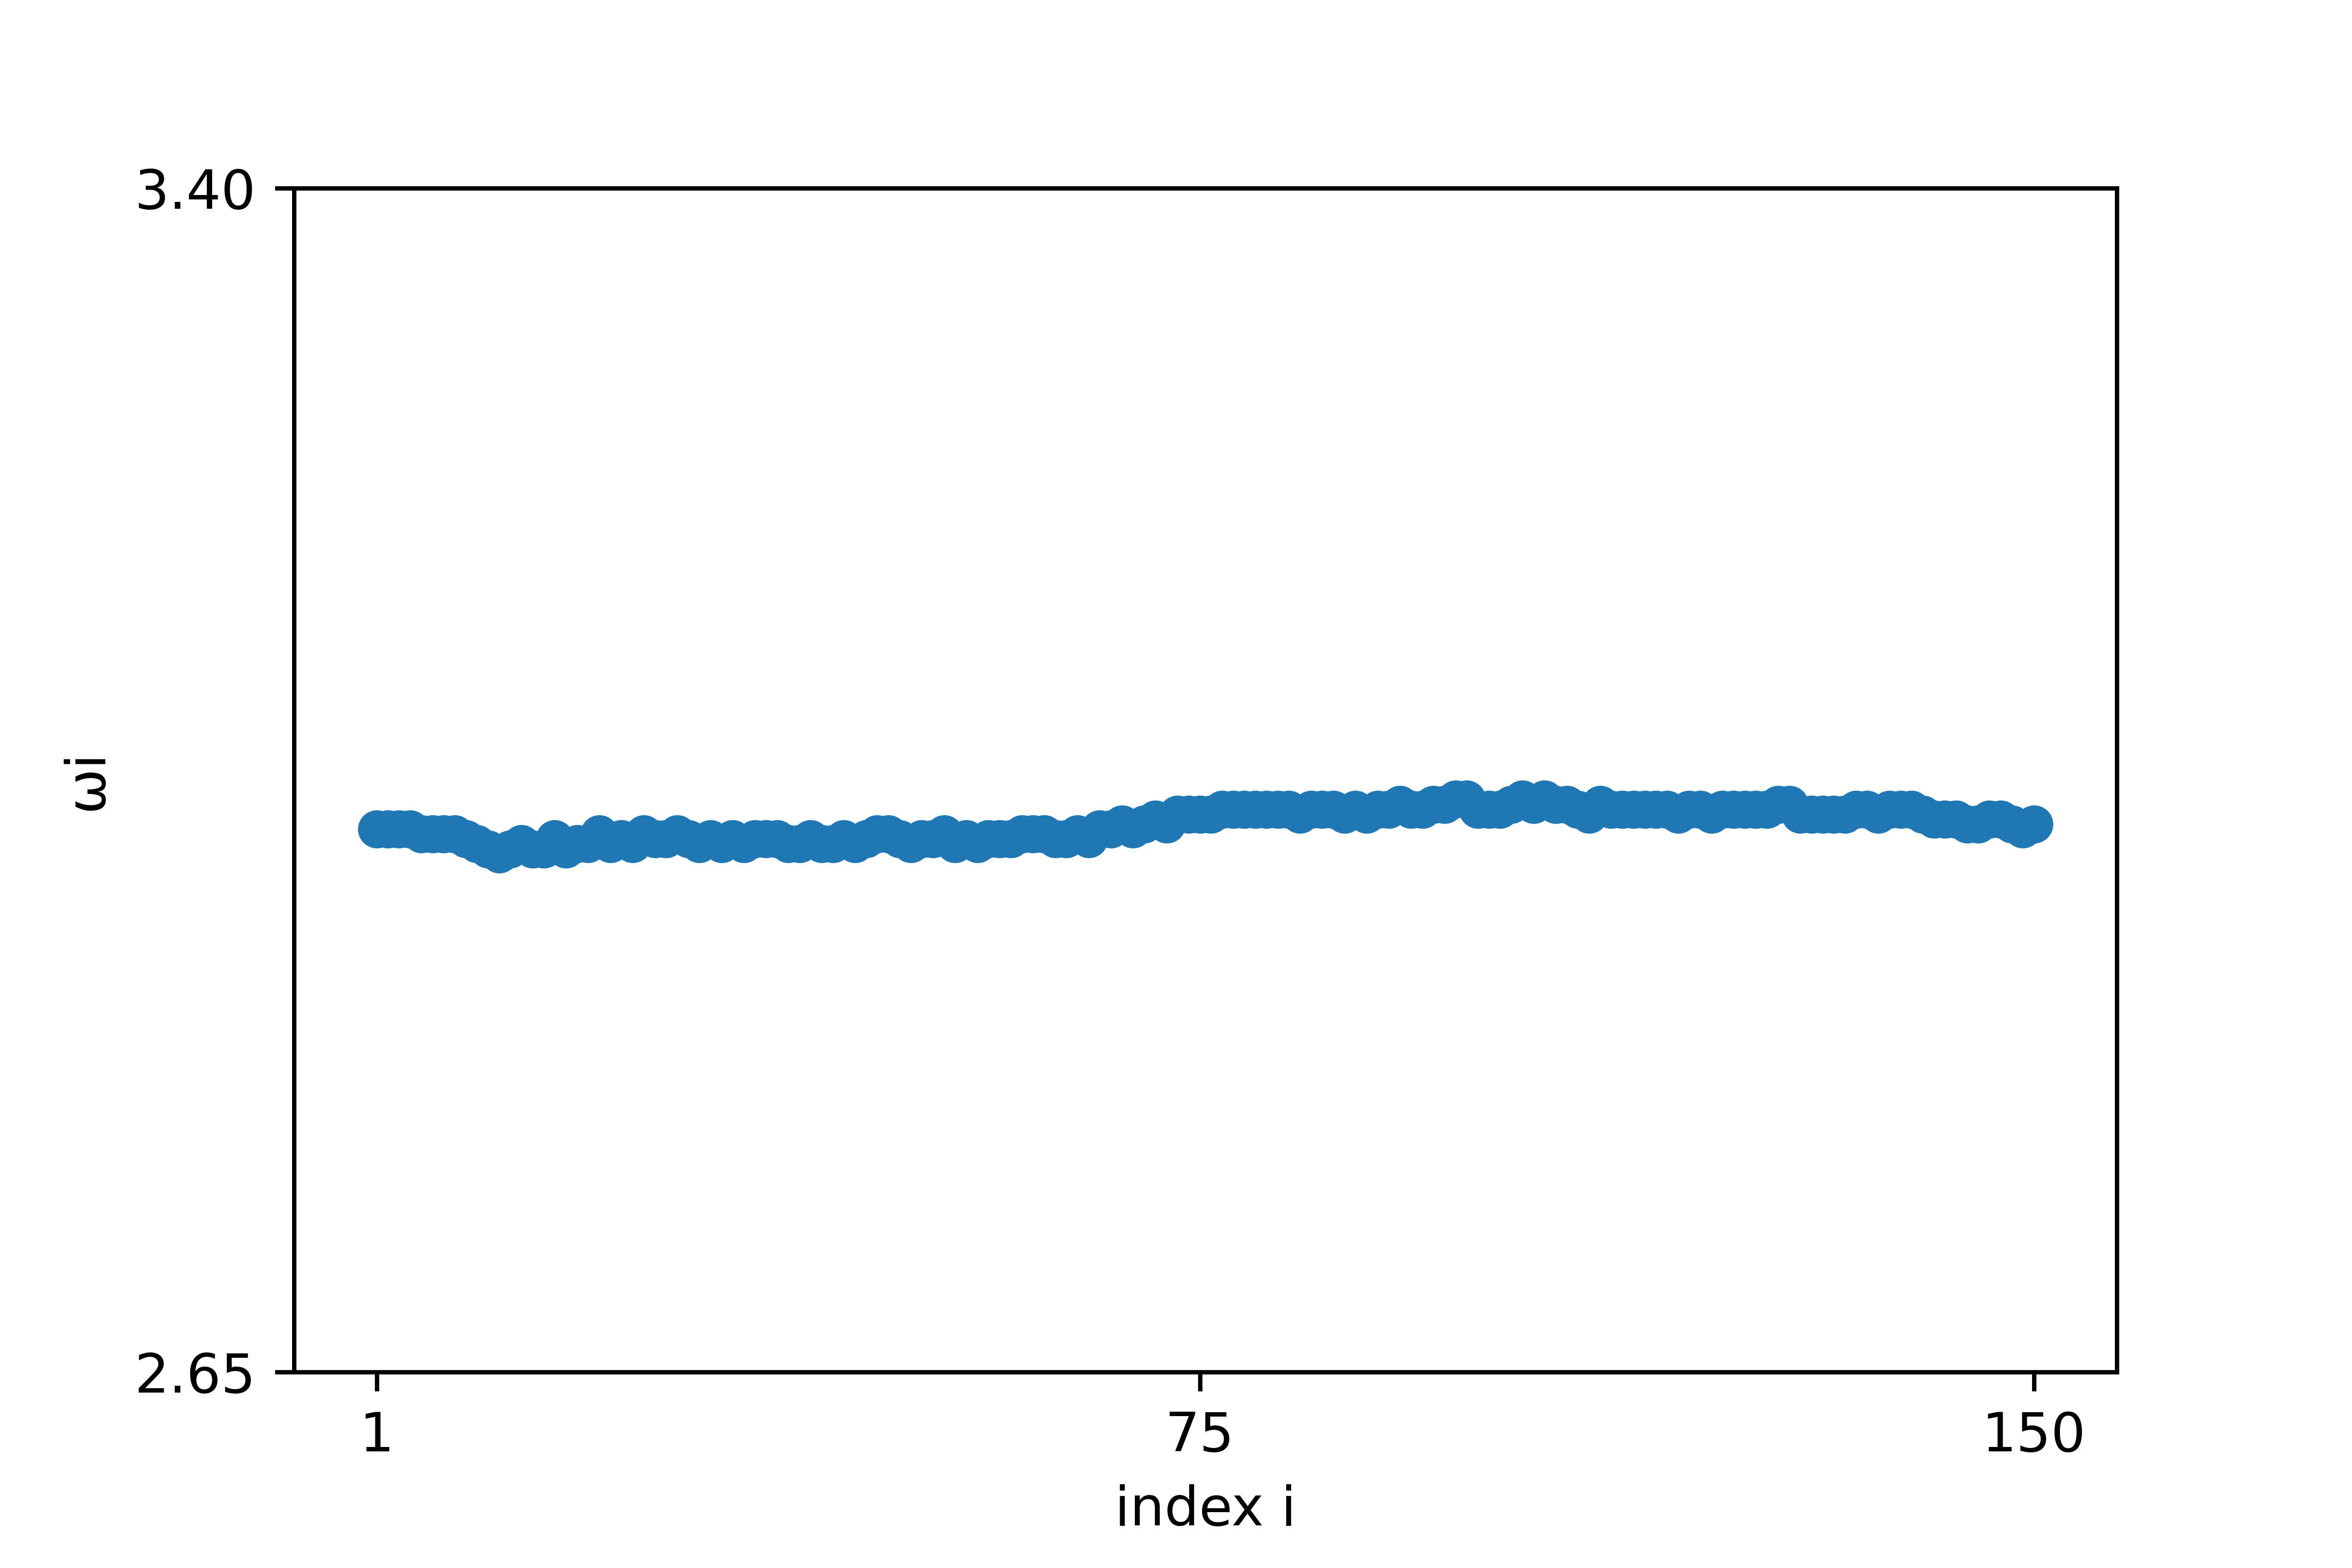
\includegraphics[width=1\linewidth]{w_lambda=0.96_t=2000.png}  
  \caption{$\lambda=0.96$}
\end{subfigure}
\hfill
\begin{subfigure}{.32\textwidth}
  \centering
  % include first image
  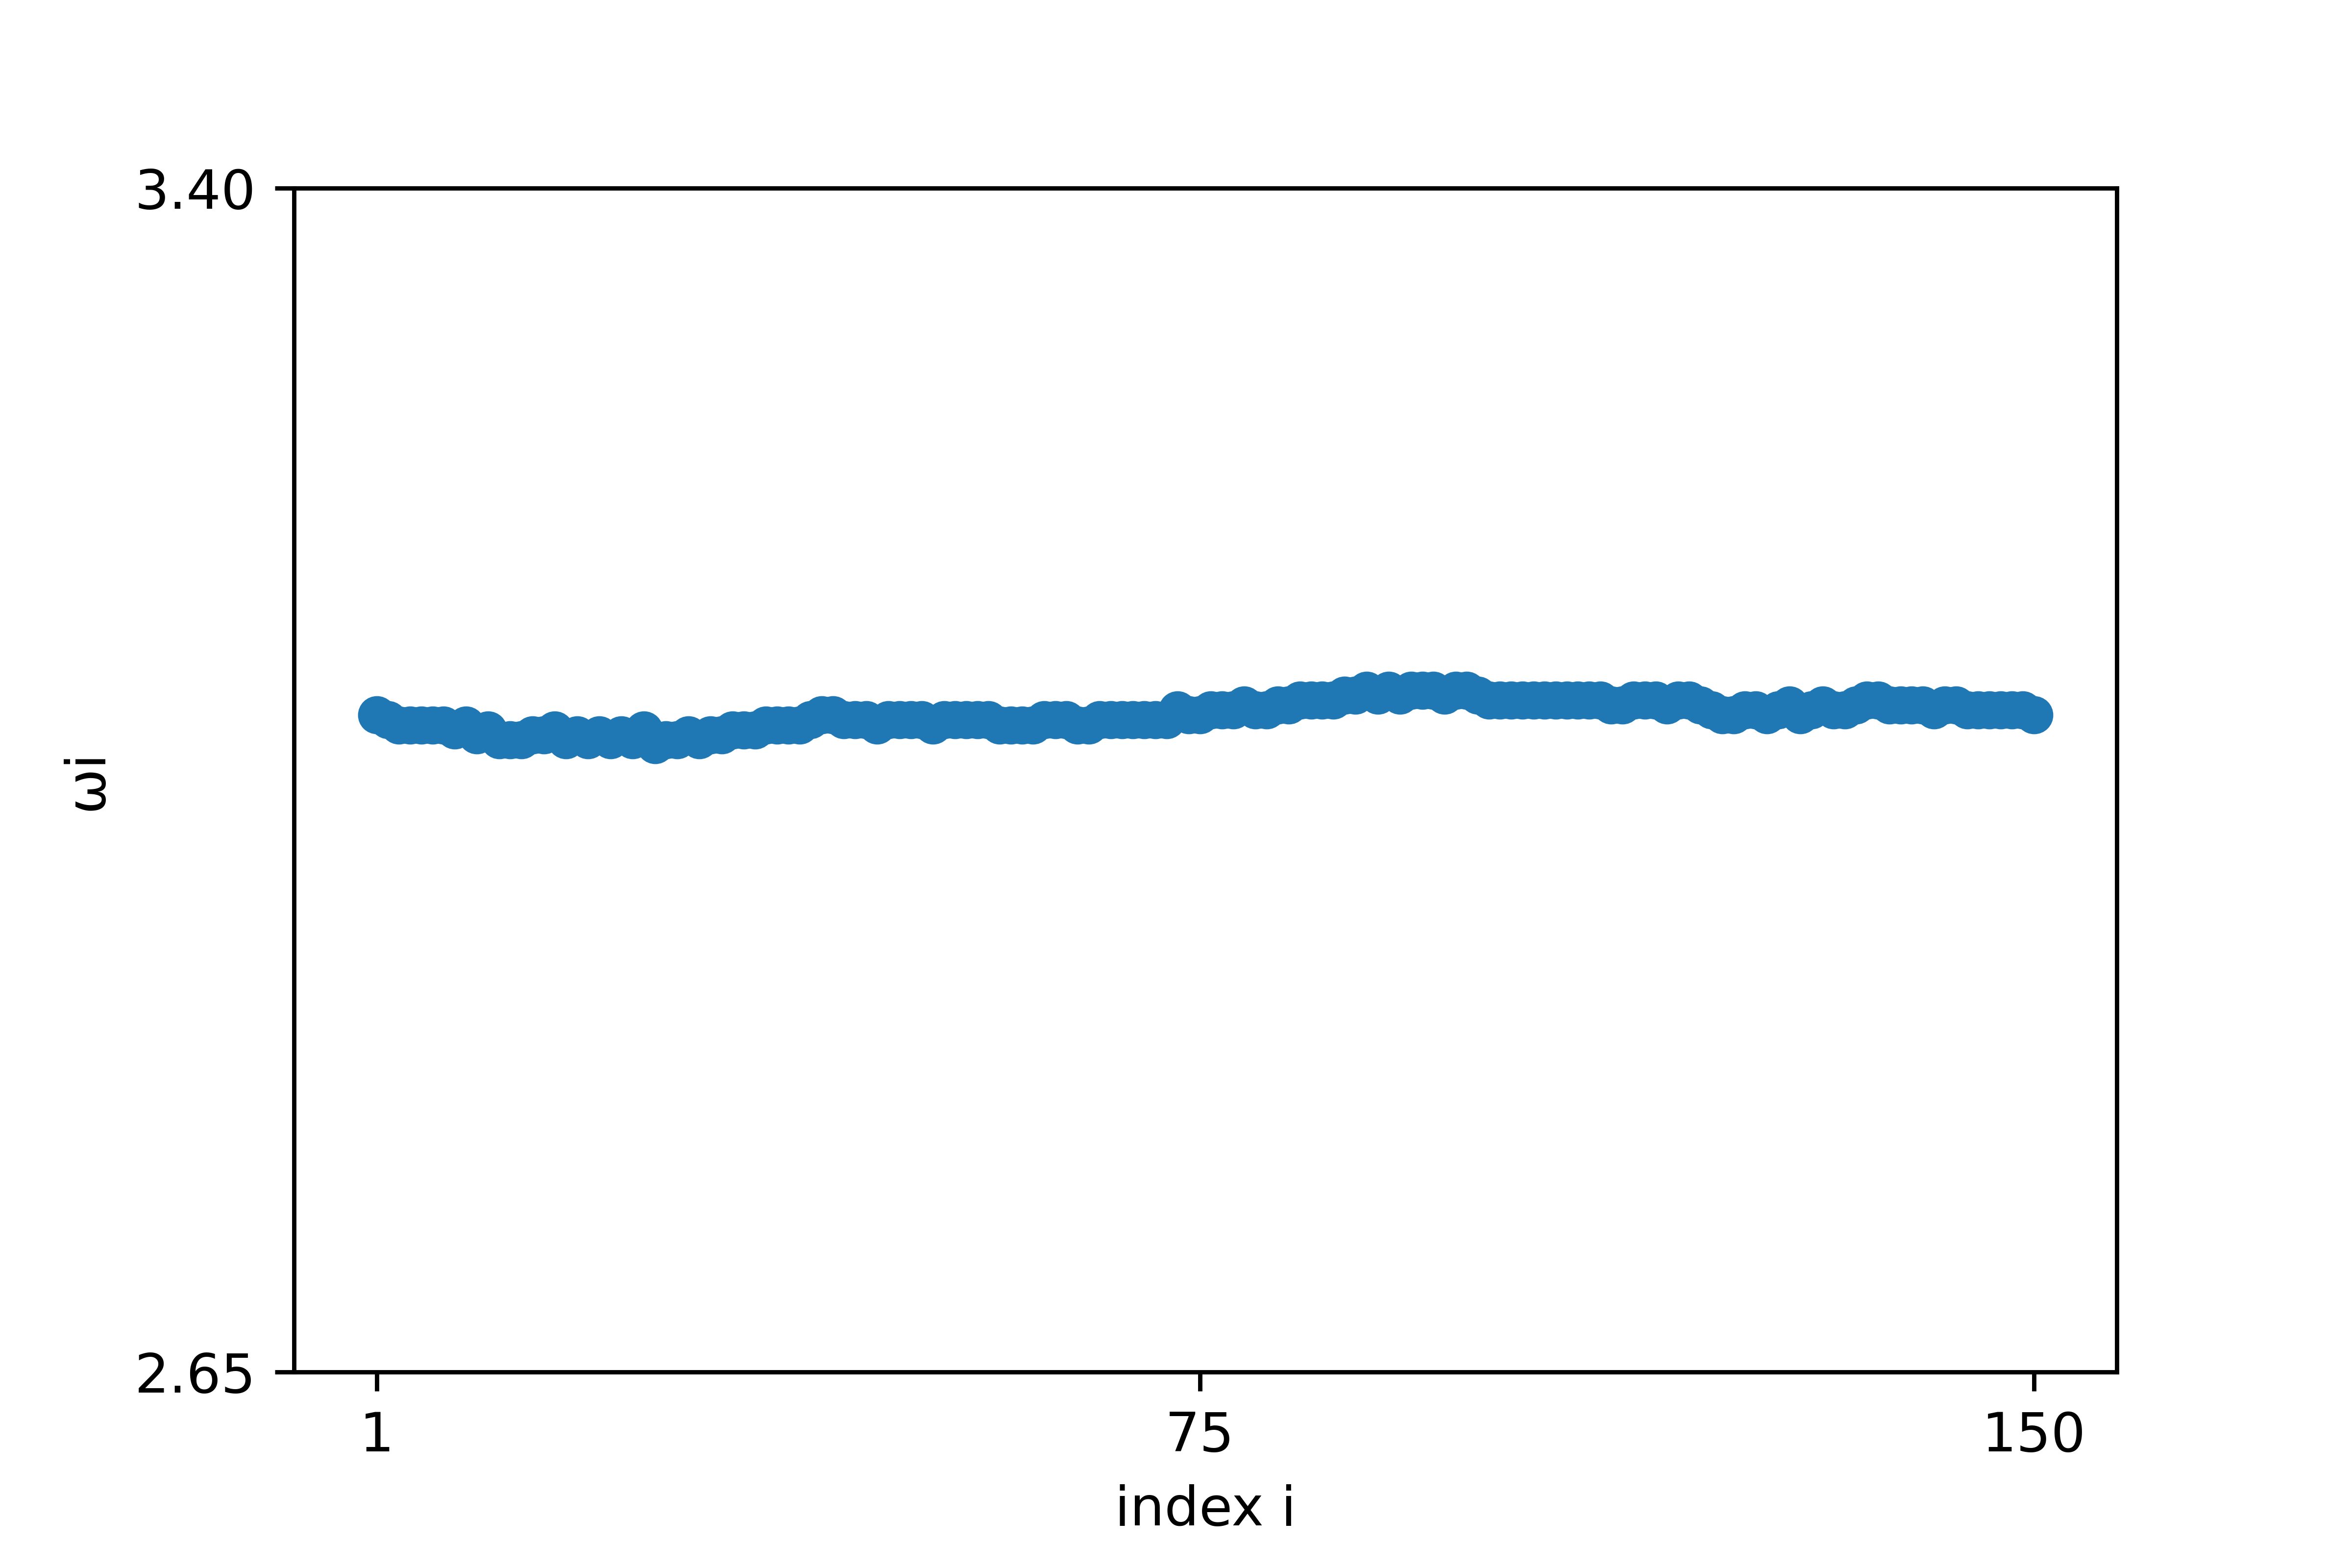
\includegraphics[width=1\linewidth]{w_lambda=0.95_t=2000.png}  
  \caption{$\lambda=0.95$}
\end{subfigure}

\begin{subfigure}{.32\textwidth}
  \centering
  % include first image
  \includegraphics[width=1\linewidth]{w_lambda=0.94_t=2000.png}  
  \caption{$\lambda=0.94$}
\end{subfigure}
\hfill
\begin{subfigure}{.32\textwidth}
  \centering
  % include second image
  \includegraphics[width=1\linewidth]{w_lambda=0.93_t=2000.png}  
  \caption{$\lambda=0.93$}
\end{subfigure}
\hfill
\begin{subfigure}{.32\textwidth}
  \centering
  % include first image
  \includegraphics[width=1\linewidth]{w_lambda=0.92_t=2000}  
  \caption{$\lambda=0.92$}
\end{subfigure}
\centering
\begin{subfigure}{.32\textwidth}
  \centering
  % include first image
  \includegraphics[width=1\linewidth]{w_lambda=0.91_t=2000.png}  
  \caption{$\lambda=0.91$}
\end{subfigure}
\begin{subfigure}{.32\textwidth}
  \centering
  % include first image
  \includegraphics[width=1\linewidth]{w_lambda=0.9_t=2000.png}  
  \caption{$\lambda=0.90$}
\end{subfigure}

\caption{Mean phase-velocity profiles $\omega_i$ at $t=2000$ time units, for $N=150$, $r=0.4$ and $\sigma = 0.7$ and for various values of $\lambda$.}
\label{uivslmd2}
\end{figure}

\section{Conclusions}
Chimera states on a non-locally coupled network of LIF neurons highly depends on the coupling strength and the coupling range. The analysis of networks of around $N=100$ neurons has shown the apperance of chimeras for intermediate values of coupling strength, for a large enough value of the coupling range. In addition, we observed that when we double the coupling strength, the single chimera becomes a double chimera. Finally, we observed that chimeras, as well as their duration, are highly dependent on initial conditions.
\par A similar investigation can be done to include the effect of a refractory period for the neuron. For example, it has been shown \cite{tsigkrimulti} that the refractory period helps chimeras survive for longer periods and is responsible for the formation of chimeras with multiple coherent and incoherent regions. Future work should address quantitative investigation of the parameter regions which favour chimera states and could include additional parameters related to the experimentally measured time-scales of biological neurons.

\section{Appendix: Python script}

\lstinputlisting[language=Python]{runner.py}


\addcontentsline{toc}{section}{References}

\pagebreak

\begin{thebibliography}{30}

\bibitem{kuramoto}
Y. Kuramoto and D. Battogtokh. Coexistence of coherence and incoherence in nonlocally coupled phase oscillators. Nonlin. Phen. in Complex Sys., 5:380-385, 2002.

\bibitem{stro}
D. M. Abrams, S. H. Strogatz. Chimera states for coupled oscillators. Phys. Rev. Lett., 93:174102, 2004.

\bibitem{tsigkrimulti}
N. D. Tsigkri-DeSmedt, J. Hizanidis, P. H{\"o}vel, A. Provata. Multi-chimera states and transitions in the leaky integrate-and-fire model with nonlocal and hierarchical connectivity. Eur. Phys. J. Spec. Top., 225:1149–1164, 2016.

\bibitem{tsigkrimulti2}
N. D. Tsigkri-DeSmedt, J. Hizanidis, P. H{\"o}vel, A. Provata. Multi-chimera states in the leaky integrate-and-fire model. Procedia Computer Sci., 66:13-22, 2015.

\bibitem{tsigkrichim}
N. D. Tsigkri-DeSmedt, J. Hizanidis, E. Sch{\"o}ll, A. Provata. Chimeras in leaky integrate-and-fire neural networks: effects of reflecting connectivities. Eur. Phys. J. B, 90:139, 2017.

\end{thebibliography}



\end{document}